
\documentclass[12pt,twoside,phd]{dms}

\usepackage[utf8]{inputenc} %
\usepackage[T1]{fontenc}    %
\usepackage{textcomp}

\usepackage{lmodern}

\francais %


\def\sloppy{%
  \tolerance 500%
  \emergencystretch 3em%
  \hfuzz .5pt
  \vfuzz\hfuzz}
\sloppy   %

\usepackage{graphicx,amssymb,icomma}


\usepackage[labelfont=bf, width=\linewidth]{caption}

\usepackage{hyperref}  %
\hypersetup{colorlinks=true,allcolors=black}
\usepackage{hypcap}   %
\usepackage{bookmark} %


\newtheorem{cor}{\corollaryname}[section]
\newtheorem{deff}[cor]{\definitionname}
\newtheorem{ex}[cor]{\examplename}
\newtheorem{lem}[cor]{\lemmaname}
\newtheorem{proposition}[cor]{Proposition}
\newtheorem{prop}[cor]{Proposition}
\newtheorem{rem}[cor]{\remarkname}
\newtheorem{theo}[cor]{\theoremname}
\theoremstyle{definition}
\newtheorem{algo}[cor]{\algoname}



\numberwithin{equation}{section}
\numberwithin{table}{chapter}
\numberwithin{figure}{chapter}

\usepackage{float}



\usepackage[onehalfspacing]{setspace}

\usepackage{natbib}

\usepackage{mathptmx}
\usepackage{nicefrac}
\usepackage{thmtools, thm-restate}

\usepackage{xspace}

\usepackage{lscape}  %

\usepackage{threeparttable} %

\usepackage{dcolumn,amsmath}

\usepackage{amsfonts}
\usepackage{amsthm}

\usepackage{epsfig}


\usepackage{makecell}


\usepackage{amsmath,amsfonts,bm}

\newcommand{\figleft}{{\em (Left)}}
\newcommand{\figcenter}{{\em (Center)}}
\newcommand{\figright}{{\em (Right)}}
\newcommand{\figtop}{{\em (Top)}}
\newcommand{\figbottom}{{\em (Bottom)}}
\newcommand{\captiona}{{\em (a)}}
\newcommand{\captionb}{{\em (b)}}
\newcommand{\captionc}{{\em (c)}}
\newcommand{\captiond}{{\em (d)}}

\newcommand{\newterm}[1]{{\bf #1}}


\def\figref#1{figure~\ref{#1}}
\def\Figref#1{Figure~\ref{#1}}
\def\twofigref#1#2{figures \ref{#1} and \ref{#2}}
\def\quadfigref#1#2#3#4{figures \ref{#1}, \ref{#2}, \ref{#3} and \ref{#4}}
\def\secref#1{section~\ref{#1}}
\def\Secref#1{Section~\ref{#1}}
\def\twosecrefs#1#2{sections \ref{#1} and \ref{#2}}
\def\secrefs#1#2#3{sections \ref{#1}, \ref{#2} and \ref{#3}}
\def\eqref#1{eq.~\ref{#1}}
\def\Eqref#1{Eq.~\ref{#1}}
\def\plaineqref#1{\ref{#1}}
\def\chapref#1{chapter~\ref{#1}}
\def\Chapref#1{Chapter~\ref{#1}}
\def\rangechapref#1#2{chapters\ref{#1}--\ref{#2}}
\def\algref#1{algorithm~\ref{#1}}
\def\Algref#1{Algorithm~\ref{#1}}
\def\twoalgref#1#2{algorithms \ref{#1} and \ref{#2}}
\def\Twoalgref#1#2{Algorithms \ref{#1} and \ref{#2}}
\def\partref#1{part~\ref{#1}}
\def\Partref#1{Part~\ref{#1}}
\def\twopartref#1#2{parts \ref{#1} and \ref{#2}}

\def\ceil#1{\lceil #1 \rceil}
\def\floor#1{\lfloor #1 \rfloor}
\def\1{\bm{1}}
\newcommand{\train}{\mathcal{D}}
\newcommand{\valid}{\mathcal{D_{\mathrm{valid}}}}
\newcommand{\test}{\mathcal{D_{\mathrm{test}}}}

\def\eps{{\epsilon}}


\def\reta{{\textnormal{$\eta$}}}
\def\ra{{\textnormal{a}}}
\def\rb{{\textnormal{b}}}
\def\rc{{\textnormal{c}}}
\def\rd{{\textnormal{d}}}
\def\re{{\textnormal{e}}}
\def\rf{{\textnormal{f}}}
\def\rg{{\textnormal{g}}}
\def\rh{{\textnormal{h}}}
\def\ri{{\textnormal{i}}}
\def\rj{{\textnormal{j}}}
\def\rk{{\textnormal{k}}}
\def\rl{{\textnormal{l}}}
\def\rn{{\textnormal{n}}}
\def\ro{{\textnormal{o}}}
\def\rp{{\textnormal{p}}}
\def\rq{{\textnormal{q}}}
\def\rr{{\textnormal{r}}}
\def\rs{{\textnormal{s}}}
\def\rt{{\textnormal{t}}}
\def\ru{{\textnormal{u}}}
\def\rv{{\textnormal{v}}}
\def\rw{{\textnormal{w}}}
\def\rx{{\textnormal{x}}}
\def\ry{{\textnormal{y}}}
\def\rz{{\textnormal{z}}}

\def\rvepsilon{{\mathbf{\epsilon}}}
\def\rvtheta{{\mathbf{\theta}}}
\def\rva{{\mathbf{a}}}
\def\rvb{{\mathbf{b}}}
\def\rvc{{\mathbf{c}}}
\def\rvd{{\mathbf{d}}}
\def\rve{{\mathbf{e}}}
\def\rvf{{\mathbf{f}}}
\def\rvg{{\mathbf{g}}}
\def\rvh{{\mathbf{h}}}
\def\rvu{{\mathbf{i}}}
\def\rvj{{\mathbf{j}}}
\def\rvk{{\mathbf{k}}}
\def\rvl{{\mathbf{l}}}
\def\rvm{{\mathbf{m}}}
\def\rvn{{\mathbf{n}}}
\def\rvo{{\mathbf{o}}}
\def\rvp{{\mathbf{p}}}
\def\rvq{{\mathbf{q}}}
\def\rvr{{\mathbf{r}}}
\def\rvs{{\mathbf{s}}}
\def\rvt{{\mathbf{t}}}
\def\rvu{{\mathbf{u}}}
\def\rvv{{\mathbf{v}}}
\def\rvw{{\mathbf{w}}}
\def\rvx{{\mathbf{x}}}
\def\rvy{{\mathbf{y}}}
\def\rvz{{\mathbf{z}}}

\def\erva{{\textnormal{a}}}
\def\ervb{{\textnormal{b}}}
\def\ervc{{\textnormal{c}}}
\def\ervd{{\textnormal{d}}}
\def\erve{{\textnormal{e}}}
\def\ervf{{\textnormal{f}}}
\def\ervg{{\textnormal{g}}}
\def\ervh{{\textnormal{h}}}
\def\ervi{{\textnormal{i}}}
\def\ervj{{\textnormal{j}}}
\def\ervk{{\textnormal{k}}}
\def\ervl{{\textnormal{l}}}
\def\ervm{{\textnormal{m}}}
\def\ervn{{\textnormal{n}}}
\def\ervo{{\textnormal{o}}}
\def\ervp{{\textnormal{p}}}
\def\ervq{{\textnormal{q}}}
\def\ervr{{\textnormal{r}}}
\def\ervs{{\textnormal{s}}}
\def\ervt{{\textnormal{t}}}
\def\ervu{{\textnormal{u}}}
\def\ervv{{\textnormal{v}}}
\def\ervw{{\textnormal{w}}}
\def\ervx{{\textnormal{x}}}
\def\ervy{{\textnormal{y}}}
\def\ervz{{\textnormal{z}}}

\def\rmSS{{\mathrm{\Sigma}}}

\def\rmA{{\mathbf{A}}}
\def\rmB{{\mathbf{B}}}
\def\rmC{{\mathbf{C}}}
\def\rmD{{\mathbf{D}}}
\def\rmE{{\mathbf{E}}}
\def\rmF{{\mathbf{F}}}
\def\rmG{{\mathbf{G}}}
\def\rmH{{\mathbf{H}}}
\def\rmI{{\mathbf{I}}}
\def\rmJ{{\mathbf{J}}}
\def\rmK{{\mathbf{K}}}
\def\rmL{{\mathbf{L}}}
\def\rmM{{\mathbf{M}}}
\def\rmN{{\mathbf{N}}}
\def\rmO{{\mathbf{O}}}
\def\rmP{{\mathbf{P}}}
\def\rmQ{{\mathbf{Q}}}
\def\rmR{{\mathbf{R}}}
\def\rmS{{\mathbf{S}}}
\def\rmT{{\mathbf{T}}}
\def\rmU{{\mathbf{U}}}
\def\rmV{{\mathbf{V}}}
\def\rmW{{\mathbf{W}}}
\def\rmX{{\mathbf{X}}}
\def\rmY{{\mathbf{Y}}}
\def\rmZ{{\mathbf{Z}}}

\def\ermA{{\textnormal{A}}}
\def\ermB{{\textnormal{B}}}
\def\ermC{{\textnormal{C}}}
\def\ermD{{\textnormal{D}}}
\def\ermE{{\textnormal{E}}}
\def\ermF{{\textnormal{F}}}
\def\ermG{{\textnormal{G}}}
\def\ermH{{\textnormal{H}}}
\def\ermI{{\textnormal{I}}}
\def\ermJ{{\textnormal{J}}}
\def\ermK{{\textnormal{K}}}
\def\ermL{{\textnormal{L}}}
\def\ermM{{\textnormal{M}}}
\def\ermN{{\textnormal{N}}}
\def\ermO{{\textnormal{O}}}
\def\ermP{{\textnormal{P}}}
\def\ermQ{{\textnormal{Q}}}
\def\ermR{{\textnormal{R}}}
\def\ermS{{\textnormal{S}}}
\def\ermT{{\textnormal{T}}}
\def\ermU{{\textnormal{U}}}
\def\ermV{{\textnormal{V}}}
\def\ermW{{\textnormal{W}}}
\def\ermX{{\textnormal{X}}}
\def\ermY{{\textnormal{Y}}}
\def\ermZ{{\textnormal{Z}}}

\def\vzero{{\bm{0}}}
\def\vone{{\bm{1}}}
\def\vmu{{\bm{\mu}}}
\def\vtheta{{\bm{\theta}}}
\def\va{{\bm{a}}}
\def\vb{{\bm{b}}}
\def\vc{{\bm{c}}}
\def\vd{{\bm{d}}}
\def\ve{{\bm{e}}}
\def\vf{{\bm{f}}}
\def\vg{{\bm{g}}}
\def\vh{{\bm{h}}}
\def\vi{{\bm{i}}}
\def\vj{{\bm{j}}}
\def\vk{{\bm{k}}}
\def\vl{{\bm{l}}}
\def\vm{{\bm{m}}}
\def\vn{{\bm{n}}}
\def\vo{{\bm{o}}}
\def\vp{{\bm{p}}}
\def\vq{{\bm{q}}}
\def\vr{{\bm{r}}}
\def\vs{{\bm{s}}}
\def\vt{{\bm{t}}}
\def\vu{{\bm{u}}}
\def\vv{{\bm{v}}}
\def\vw{{\bm{w}}}
\def\vx{{\bm{x}}}
\def\vy{{\bm{y}}}
\def\vz{{\bm{z}}}

\def\evalpha{{\alpha}}
\def\evbeta{{\beta}}
\def\evepsilon{{\epsilon}}
\def\evlambda{{\lambda}}
\def\evomega{{\omega}}
\def\evmu{{\mu}}
\def\evpsi{{\psi}}
\def\evsigma{{\sigma}}
\def\evtheta{{\theta}}
\def\eva{{a}}
\def\evb{{b}}
\def\evc{{c}}
\def\evd{{d}}
\def\eve{{e}}
\def\evf{{f}}
\def\evg{{g}}
\def\evh{{h}}
\def\evi{{i}}
\def\evj{{j}}
\def\evk{{k}}
\def\evl{{l}}
\def\evm{{m}}
\def\evn{{n}}
\def\evo{{o}}
\def\evp{{p}}
\def\evq{{q}}
\def\evr{{r}}
\def\evs{{s}}
\def\evt{{t}}
\def\evu{{u}}
\def\evv{{v}}
\def\evw{{w}}
\def\evx{{x}}
\def\evy{{y}}
\def\evz{{z}}

\def\mA{{\bm{A}}}
\def\mB{{\bm{B}}}
\def\mC{{\bm{C}}}
\def\mD{{\bm{D}}}
\def\mE{{\bm{E}}}
\def\mF{{\bm{F}}}
\def\mG{{\bm{G}}}
\def\mH{{\bm{H}}}
\def\mI{{\bm{I}}}
\def\mJ{{\bm{J}}}
\def\mK{{\bm{K}}}
\def\mL{{\bm{L}}}
\def\mM{{\bm{M}}}
\def\mN{{\bm{N}}}
\def\mO{{\bm{O}}}
\def\mP{{\bm{P}}}
\def\mQ{{\bm{Q}}}
\def\mR{{\bm{R}}}
\def\mS{{\bm{S}}}
\def\mT{{\bm{T}}}
\def\mU{{\bm{U}}}
\def\mV{{\bm{V}}}
\def\mW{{\bm{W}}}
\def\mX{{\bm{X}}}
\def\mY{{\bm{Y}}}
\def\mZ{{\bm{Z}}}
\def\mBeta{{\bm{\beta}}}
\def\mPhi{{\bm{\Phi}}}
\def\mLambda{{\bm{\Lambda}}}
\def\mSigma{{\bm{\Sigma}}}

\DeclareMathAlphabet{\mathsfit}{\encodingdefault}{\sfdefault}{m}{sl}
\SetMathAlphabet{\mathsfit}{bold}{\encodingdefault}{\sfdefault}{bx}{n}
\newcommand{\tens}[1]{\bm{\mathsfit{#1}}}
\def\tA{{\tens{A}}}
\def\tB{{\tens{B}}}
\def\tC{{\tens{C}}}
\def\tD{{\tens{D}}}
\def\tE{{\tens{E}}}
\def\tF{{\tens{F}}}
\def\tG{{\tens{G}}}
\def\tH{{\tens{H}}}
\def\tI{{\tens{I}}}
\def\tJ{{\tens{J}}}
\def\tK{{\tens{K}}}
\def\tL{{\tens{L}}}
\def\tM{{\tens{M}}}
\def\tN{{\tens{N}}}
\def\tO{{\tens{O}}}
\def\tP{{\tens{P}}}
\def\tQ{{\tens{Q}}}
\def\tR{{\tens{R}}}
\def\tS{{\tens{S}}}
\def\tT{{\tens{T}}}
\def\tU{{\tens{U}}}
\def\tV{{\tens{V}}}
\def\tW{{\tens{W}}}
\def\tX{{\tens{X}}}
\def\tY{{\tens{Y}}}
\def\tZ{{\tens{Z}}}


\def\gA{{\mathcal{A}}}
\def\gB{{\mathcal{B}}}
\def\gC{{\mathcal{C}}}
\def\gD{{\mathcal{D}}}
\def\gE{{\mathcal{E}}}
\def\gF{{\mathcal{F}}}
\def\gG{{\mathcal{G}}}
\def\gH{{\mathcal{H}}}
\def\gI{{\mathcal{I}}}
\def\gJ{{\mathcal{J}}}
\def\gK{{\mathcal{K}}}
\def\gL{{\mathcal{L}}}
\def\gM{{\mathcal{M}}}
\def\gN{{\mathcal{N}}}
\def\gO{{\mathcal{O}}}
\def\gP{{\mathcal{P}}}
\def\gQ{{\mathcal{Q}}}
\def\gR{{\mathcal{R}}}
\def\gS{{\mathcal{S}}}
\def\gT{{\mathcal{T}}}
\def\gU{{\mathcal{U}}}
\def\gV{{\mathcal{V}}}
\def\gW{{\mathcal{W}}}
\def\gX{{\mathcal{X}}}
\def\gY{{\mathcal{Y}}}
\def\gZ{{\mathcal{Z}}}

\def\sA{{\mathbb{A}}}
\def\sB{{\mathbb{B}}}
\def\sC{{\mathbb{C}}}
\def\sD{{\mathbb{D}}}
\def\sF{{\mathbb{F}}}
\def\sG{{\mathbb{G}}}
\def\sH{{\mathbb{H}}}
\def\sI{{\mathbb{I}}}
\def\sJ{{\mathbb{J}}}
\def\sK{{\mathbb{K}}}
\def\sL{{\mathbb{L}}}
\def\sM{{\mathbb{M}}}
\def\sN{{\mathbb{N}}}
\def\sO{{\mathbb{O}}}
\def\sP{{\mathbb{P}}}
\def\sQ{{\mathbb{Q}}}
\def\sR{{\mathbb{R}}}
\def\sS{{\mathbb{S}}}
\def\sT{{\mathbb{T}}}
\def\sU{{\mathbb{U}}}
\def\sV{{\mathbb{V}}}
\def\sW{{\mathbb{W}}}
\def\sX{{\mathbb{X}}}
\def\sY{{\mathbb{Y}}}
\def\sZ{{\mathbb{Z}}}

\def\emLambda{{\Lambda}}
\def\emA{{A}}
\def\emB{{B}}
\def\emC{{C}}
\def\emD{{D}}
\def\emE{{E}}
\def\emF{{F}}
\def\emG{{G}}
\def\emH{{H}}
\def\emI{{I}}
\def\emJ{{J}}
\def\emK{{K}}
\def\emL{{L}}
\def\emM{{M}}
\def\emN{{N}}
\def\emO{{O}}
\def\emP{{P}}
\def\emQ{{Q}}
\def\emR{{R}}
\def\emS{{S}}
\def\emT{{T}}
\def\emU{{U}}
\def\emV{{V}}
\def\emW{{W}}
\def\emX{{X}}
\def\emY{{Y}}
\def\emZ{{Z}}
\def\emSigma{{\Sigma}}

\newcommand{\etens}[1]{\mathsfit{#1}}
\def\etLambda{{\etens{\Lambda}}}
\def\etA{{\etens{A}}}
\def\etB{{\etens{B}}}
\def\etC{{\etens{C}}}
\def\etD{{\etens{D}}}
\def\etE{{\etens{E}}}
\def\etF{{\etens{F}}}
\def\etG{{\etens{G}}}
\def\etH{{\etens{H}}}
\def\etI{{\etens{I}}}
\def\etJ{{\etens{J}}}
\def\etK{{\etens{K}}}
\def\etL{{\etens{L}}}
\def\etM{{\etens{M}}}
\def\etN{{\etens{N}}}
\def\etO{{\etens{O}}}
\def\etP{{\etens{P}}}
\def\etQ{{\etens{Q}}}
\def\etR{{\etens{R}}}
\def\etS{{\etens{S}}}
\def\etT{{\etens{T}}}
\def\etU{{\etens{U}}}
\def\etV{{\etens{V}}}
\def\etW{{\etens{W}}}
\def\etX{{\etens{X}}}
\def\etY{{\etens{Y}}}
\def\etZ{{\etens{Z}}}

\newcommand{\pdata}{p_{\rm{data}}}
\newcommand{\ptrain}{\hat{p}_{\rm{data}}}
\newcommand{\Ptrain}{\hat{P}_{\rm{data}}}
\newcommand{\pmodel}{p_{\rm{model}}}
\newcommand{\Pmodel}{P_{\rm{model}}}
\newcommand{\ptildemodel}{\tilde{p}_{\rm{model}}}
\newcommand{\pencode}{p_{\rm{encoder}}}
\newcommand{\pdecode}{p_{\rm{decoder}}}
\newcommand{\precons}{p_{\rm{reconstruct}}}

\newcommand{\laplace}{\mathrm{Laplace}} %

\newcommand{\E}{\mathbb{E}}
\newcommand{\Ls}{\mathcal{L}}
\newcommand{\R}{\mathbb{R}}
\newcommand{\emp}{\tilde{p}}
\newcommand{\lr}{\alpha}
\newcommand{\reg}{\lambda}
\newcommand{\rect}{\mathrm{rectifier}}
\newcommand{\softmax}{\mathrm{softmax}}
\newcommand{\sigmoid}{\sigma}
\newcommand{\softplus}{\zeta}
\newcommand{\KL}{\gD_{\mathrm{KL}}}
\newcommand{\Var}{\mathrm{Var}}
\newcommand{\standarderror}{\mathrm{SE}}
\newcommand{\Cov}{\mathrm{Cov}}
\newcommand{\V}{\mathbb{V}}
\newcommand{\normlzero}{L^0}
\newcommand{\normlone}{L^1}
\newcommand{\normltwo}{L^2}
\newcommand{\normlp}{L^p}
\newcommand{\normmax}{L^\infty}

\newcommand{\parents}{Pa} %

\DeclareMathOperator*{\argmax}{arg\,max}
\DeclareMathOperator*{\argmin}{arg\,min}

\DeclareMathOperator{\sign}{sign}
\DeclareMathOperator{\Tr}{Tr}
\let\ab\allowbreak



\newcommand{\defas}{\stackrel{\text{def}}{=}}
\newcommand{\RR}{\mathbb{R}}

\usepackage{xspace}
\usepackage{lscape}  %

\usepackage{cleveref}
\usepackage{threeparttable} %
\usepackage{wrapfig}
\usepackage{array}
\usepackage{graphicx}
\usepackage{bbm}
\usepackage[x11names,table]{xcolor}
\usepackage{soul}
\usepackage{caption}
\usepackage{subcaption}
\usepackage{heuristica}
\usepackage{dcolumn}
\usepackage{float}
\usepackage{amsfonts}
\usepackage{amsthm}
\usepackage{booktabs} %
\usepackage{amsmath}
\usepackage{amssymb, bbm}
\usepackage{tikz}
\usepackage{tkz-euclide}
\usetikzlibrary{fit, positioning, arrows, automata, decorations.pathmorphing}
\usepackage{algorithm}
\usepackage{algorithmic}
%\usepackage{algcompatible}
\usepackage{mathtools}
\usepackage{epsfig}
\usepackage{adjustbox}
\newcommand{\kl}[2]{\gD_{\textsc{KL}}\big(#1||#2\big)}

\usepackage{enumitem}

\setlist[itemize]{label=\textbullet}

\definecolor{right}{HTML}{697c2a}
\definecolor{down}{HTML}{000000}



\definecolor{alpha}{RGB}{234, 186, 120}
\definecolor{beta}{RGB}{46, 156, 210}
\def\mathunderline#1#2{\color{#1}\underline{{\color{black}#2}}\color{black}}
\DeclareSymbolFontAlphabet{\mathbb}{AMSb}
\DeclareMathAlphabet{\mathcal}{OMS}{cmsy}{m}{n}
\newcommand{\rmodel}{r_{\text{model}}} %
\newcommand{\remove}[1]{}
\newcommand{\penv}{p_{\text{env}}} %
\newcommand{\traj}{\tau} %
\newcommand{\return}{\gR}
\newcommand{\reward}{r}
\newcommand{\Expect}{\mathop{\mathbb{E}}}
\newcommand{\parampol}{\theta} %
\newcommand{\todo}[1]{\textcolor{red}{TODO: #1}}
\newcommand{\val}[1]{\textcolor{red}{#1}}
\newcommand{\qpol}{q_\theta} 

\definecolor{airforceblue}{rgb}{0.36, 0.54, 0.66}
\definecolor{amaranth}{rgb}{0.9, 0.17, 0.31}
\definecolor{cerulean}{rgb}{0.0, 0.48, 0.65}
\definecolor{burntorange}{rgb}{0.8, 0.33, 0.0}
\definecolor{darkorchid}{rgb}{0.6, 0.2, 0.8}
\definecolor{darkterracotta}{rgb}{0.8, 0.31, 0.36}
\definecolor{dartmouthgreen}{rgb}{0.05, 0.5, 0.06}
\definecolor{darkpastelred}{rgb}{0.76, 0.23, 0.13}
\definecolor{myred}{rgb}{0.81, 0.06, 0.13}
\definecolor{myblue}{rgb}{0.15, 0.23, 0.89}
\usepackage{multirow}
\newcommand{\appropto}{\mathrel{\vcenter{
  \offinterlineskip\halign{\hfil$##$\cr
    \propto\cr\noalign{\kern2pt}\sim\cr\noalign{\kern-2pt}}}}}

\newcommand{\q}{q_\theta}
\newcommand{\logit}{\varphi_\theta}
\newcommand{\logitx}{\varphi(x ;\theta)}
\newcommand{\thetamle}{\theta^{\text{MLE}}}
\newcommand{\trhic}{\Tr{(\rmH^{-1} \rmC})}
\newcommand{\Cc}{\tilde{\rmSS}} %
\newcommand{\F}{\rmF}
\newcommand{\G}{\rmG} %

\usepackage{flafter}
\newtheorem{theorem}{Theorem}
\newtheorem{example}{Example}
\newtheorem{assumption}{Assumption}
\newtheorem{corollary}{Corollary}[theorem]
\newtheorem{lemma}{Lemma}
\newtheorem{definition}{Definition}

\usepackage{textcomp}


\usepackage{url}


\makeatletter
\renewenvironment{abstract}{%
  \if@twocolumn
    \section*{\abstractname}%
  \else
    \vspace{2em}
    \begin{center}%
      {\bfseries \abstractname\vspace{1em}\vspace{\z@}}%
    \end{center}%
    \quotation
  \fi}
{\if@twocolumn\else\endquotation\fi}
\makeatother

\linepenalty=1000

\begin{document}

\version{1}



\title{Learning and Planning with Noise in Optimization and Reinforcement Learning}

\author{Valentin Thomas}

\copyrightyear{2023}

\department{Département d'informatique et de recherche op\'{e}rationnelle}

\date{\today} %

\sujet{Informatique}

\president{Pierre-Luc Bacon}

\directeur{Yoshua Bengio}

\codirecteur{Nicolas Le Roux}         %

\membrejury{Glen Berseth}

\examinateur{Philip S. Thomas}   %



\repdoyen{Nom du représentant du doyen} %


\maketitle
\maketitle


\francais


\chapter*{R\'{e}sum\'{e}}
La plupart des algorithmes modernes d'apprentissage automatique intègrent un
certain degré d'aléatoire dans leurs processus, que nous appellerons le
\emph{bruit}, qui peut finalement avoir un impact sur les prédictions du modèle. Dans cette thèse, nous examinons de plus près l'apprentissage et la planification en présence de bruit pour les algorithmes d'apprentissage par renforcement et d'optimisation.

Les deux premiers articles présentés dans ce document se concentrent sur l'apprentissage par renforcement dans un environnement inconnu, et plus précisément sur la façon dont nous pouvons concevoir des algorithmes qui utilisent la stochasticité de leur politique et de l'environnement à leur avantage.
Notre première contribution présentée dans ce document se concentre sur le cadre
de l'apprentissage par renforcement non supervisé. Nous montrons comment un
agent laissé seul dans un monde inconnu sans but précis peut apprendre quels
aspects de l'environnement il peut contrôler indépendamment les uns des autres,
ainsi qu'apprendre conjointement une représentation latente démêlée de ces
aspects que nous appellerons \emph{facteurs de variation}.
La deuxième contribution se concentre sur la planification dans les tâches de
contrôle continu. En présentant l'apprentissage par renforcement comme un
problème d'inférence, nous empruntons des outils provenant de la littérature sur
les m\'{e}thodes de Monte Carlo séquentiel pour concevoir un algorithme efficace
et théoriquement motiv\'{e} pour la planification probabiliste en utilisant un
modèle appris du monde. Nous montrons comment l'agent peut tirer parti de note
objectif probabiliste pour imaginer divers ensembles de solutions.

Les deux contributions suivantes analysent l'impact du bruit de gradient dû à l'échantillonnage dans les algorithmes d'optimisation. 
La troisième contribution examine le rôle du bruit de l'estimateur du gradient dans l'estimation par maximum de vraisemblance avec descente de gradient stochastique, en explorant la relation entre la structure du bruit du gradient et la courbure locale sur la généralisation et la vitesse de convergence du modèle. 
Notre quatrième contribution revient sur le sujet de l'apprentissage par
renforcement pour analyser l'impact du bruit d'échantillonnage sur l'algorithme
d'optimisation de la politique par ascension du gradient. Nous constatons que le
bruit d'échantillonnage peut avoir un impact significatif sur la dynamique
d'optimisation et les politiques découvertes en apprentissage par
renforcement.


  {\bfseries Mots cl\'{e}s\hspace{-3pt}: Apprentissage de repr\'{e}sentations, Contr\^{o}le par Inf\'{e}rence Probabiliste, Apprentisage Profond par Renforcement, Planification.}
                                                                                                                                                            



\anglais
\chapter*{Abstract}

Most modern machine learning algorithms incorporate a degree of randomness in their processes, which we will refer to as noise, which can ultimately impact the model's predictions. In this thesis, we take a closer look at learning and planning in the presence of noise for reinforcement learning and optimization algorithms.

The first two articles presented in this document focus on reinforcement learning in an unknown environment, specifically how we can design algorithms that use the stochasticity of their policy and of the environment to their advantage.
Our first contribution presented in this document focuses on the unsupervised reinforcement learning setting. We show how an agent left alone in an unknown world without any specified goal can learn which aspects of the environment it can control independently from each other as well as jointly learning a disentangled latent representation of these aspects, or factors of variation.
The second contribution focuses on planning in continuous control tasks. By framing reinforcement learning as an inference problem, we borrow tools from Sequential Monte Carlo literature to design a theoretically grounded and efficient algorithm for probabilistic planning using a learned model of the world. We show how the agent can leverage the uncertainty of the model to imagine a diverse set of solutions.

The following two contributions analyze the impact of gradient noise due to sampling in optimization algorithms. 
The third contribution examines the role of gradient noise in maximum likelihood estimation with stochastic gradient descent, exploring the relationship between the structure of the gradient noise and local curvature on the generalization and convergence speed of the model. 
Our fourth contribution returns to the topic of reinforcement learning to analyze the impact of sampling noise on the policy gradient algorithm. We find that sampling noise can significantly impact the optimization dynamics and policies discovered in on-policy reinforcement learning.













\anglais
\cleardoublepage
\pdfbookmark[chapter]{\contentsname}{toc}  %
\tableofcontents
\phantomsection  %
\listoftables
\phantomsection
\listoffigures

\chapter*{Other non included works}
\val{not sure there should be a section for it or what name it should have}

\begin{itemize}
\item{\bf On the role of overparameterization in off-policy Temporal
Difference learning with linear function
approximation} (\textbf{Valentin Thomas}*). \url{https://openreview.net/forum?id=g-H3oNARs2}, {\em In {\color{blue} NeurIPS 2022}}.

\item{\bf The Role of Baselines in Policy Optimization}
    (with Jincheng Mei*, Wesley Chung, \textbf{Valentin Thomas}, Bo Dai, Csaba
    Szepesvari and Dale Schuurmans).  \url{https://arxiv.org/abs/2301.06276}, {\em In {\color{blue} NeurIPS 2022}}.
    
\item{- \bf Bridging the Gap Between Target Networks and Functional Regularization}
    (Alexandre Pich\'{e}*, \textbf{Valentin Thomas}*, Joseph Marino, Rafael Pardi\~{n}as, Gian Maria Marconi, Christopher Pal, Mohammad Emtiyaz Khan), {\em \url{https://arxiv.org/abs/2210.12282}}.

% \item{- \bf Probabilistic Planning with Sequential Monte Carlo methods}
%     (\textbf{Valentin Thomas}*, Alexandre Pich\'{e}*, Cyril Ibrahim, Yoshua
%     Bengio and Chris
%     Pal), {\em {\color{olive} Contributed talk at NeurIPS
%     2018 workshop} Infer to Control/published in {\color{blue}ICLR 2019}}.
\item{\bf Planning with Latent Simulated Trajectories} (Alexandre Pich\'{e}*, \textbf{Valentin Thomas}, Cyril Ibrahim, Yoshua Bengio, Julien Cornebise and Chris
    Pal), {\em  In {\color{olive} ICLR 2019 Workshop} on Structure \& Priors in Reinforcement
Learning}.

\item{\bf Independently Controllable Features} (Emmanuel Bengio*, \textbf{Valentin Thomas}, Joelle Pineau, Doina Precup and Yoshua Bengio), {\em In {\color{blue}RLDM 2017}}.
\end{itemize}


\chapter*{Notation and acronyms}
In this thesis we will use the convention of denoting matrices with capital bold letters. Vectors and scalars will be denoted by lowercase letters and the distinction will be made clear from context.

\section*{Notation}
\begin{table}[H]%
\begin{center}%
%\begin{tabular}{r c p{10cm} }
\begin{tabular}{r c >{\raggedright\arraybackslash}p{10cm}}
\toprule
    \multicolumn{3}{l}{\textbf{\underline{Information theory}}} \\
$X$ & $\triangleq$ & Random variable\\
$\E$ & $\triangleq$ & Expectation\\
$H(X)$ & $\triangleq$ & Entropy of $X$\\
$\gI(X,Y)$ & $\triangleq$ & Mutual information between $X$ and $Y$\\
$\KL$ & $\triangleq$ & Kullback-Leibler Divergence \\

\midrule
    \multicolumn{3}{l}{\textbf{\underline{Machine learning and reinforcement
    learning}}} \\
$\theta$ or $\phi$ & $\triangleq$ & Learnable parameters of a model\\
$\mathcal{L}$ & $\triangleq$ & Loss function\\
$\mathcal{J}$ & $\triangleq$ & Objective function to maximize\\
$s$  & $\triangleq$ & State (vector)\\
$a$  & $\triangleq$ & Action (scalar or vector)\\
$r$  & $\triangleq$ & Reward (scalar) \\
$R$  & $\triangleq$ & Return (scalar) \\
$\traj_{1:T}$ & $\triangleq$ & $\{s_i, a_i\}_{i=1}^T$ Trajectory: sequence of state-action pairs\\
$\pi$ & $\triangleq$ & A policy, i.e a distrubtion over actions given a state\\
$\gamma$ & $\triangleq$ & Discount factor\\
$\lambda$ & $\triangleq$ & Trace-decay parameter for TD($\lambda$)\\
$V^\pi$  & $\triangleq$ & Value function associated to the policy $\pi$\\
$Q^\pi$  & $\triangleq$ & State-action value function associated to the policy $\pi$\\
$\mathcal{O}_t$ & $\triangleq$ & Optimality variable used in control as
    inference\\
$\penv$ & $\triangleq$ & Transition probability of the environment\\
$\rmP$ & $\triangleq$ & Transition matrix of the environment\\
$\pmodel$ & $\triangleq$ & Model of the environment\\
$w_t$ & $\triangleq$ & Importance sampling weight\\ 

\bottomrule
\end{tabular}
\end{center}
\label{tab:notation}
\end{table}

\section*{Acronyms}
\begin{table}[H]%
\begin{center}%
\begin{tabular}{r c{10cm} }
\toprule
\textbf{Acronym} & \textbf{Full name}\\
\midrule
\textbf{ML} & Machine Learning\\
\textbf{DL} & Deep Learning\\
    \textbf{MLE} & Maximum Likelihood Estimation\\
\textbf{RL} & Reinforcement Learning\\
\textbf{DRL} & Deep Reinforcement Learning\\
\textbf{MDP} & Markov Decision Process\\
    \textbf{TD} & Temporal Difference\\
\textbf{ICF} & Independently Controllable Factors\\

\textbf{IS} & Importance Sampling\\
\textbf{MPC} & Model Predictive Control\\
    \textbf{CEM} & Cross Entropy Method\\
\textbf{HMM} & Hidden Markov Model\\
\textbf{MCTS} & Monte Carlo Tree Search\\
\textbf{MCMC} & Markov Chain Monte Carlo\\
    \textbf{SMC} & Sequential Monte Carlo\\
    \textbf{RS} & Random Shooting\\
    \textbf{SAC} & Soft Actor Critic\\
    \textbf{SG} & Stochastic Gradient\\
    \textbf{SGD} & Stochastic Gradient Descent\\
\textbf{PG} & Policy Gradient\\
\textbf{NPG} & Natural Policy Gradient\\
\bottomrule
\end{tabular}
\end{center}
\label{tab:acronyms}
\end{table}




\chapter*{Remerciements}


Famille: A ma m\`{e}re et \`{a} mon p\`{e}re pour avoir toujours \'{e}t\'{e} la, pour
avoir toujours encourage ma curiosite et tout ce que j'ai pu entreprendre
A Alicia pour

These: Yoshua, Nicolas

Stage: Philippe, Marlos, Bilal, Remi, Theophane

Amis: Alexandre, Stephanie, Gauthier, 
Salem, Victor, Ahmed, Thomas, Jules, Marc, Pierrick,
Akram
Wesley
Melissa
Veronica
Linda
Florian Strub
Simon Guiroy
Gabriel
Tristan

Flo and Meta

Audrey
Tess

Pets: Idefix, Yuki

Partner: Melodie


\NoChapterPageNumber
\cleardoublepage


\chapter{Introduction}
Learning through interaction is a fundamental aspect of natural intelligence: humans and animals learn from their experience in order to develop complex behaviors. For this reason, a primary long-term goal in the field of artificial intelligence is to create machines capable of emulating this process, able to interact with our world to perform specific tasks or achieve general objectives. Reinforcement learning (RL) is a key paradigm for learning how to interact; it is a subfield of machine learning in which an agent learns to act through trial and error. This approach has demonstrated promising results in various applications, such as games~\citep{tesauro1994td, mnih2013playing, silver2016mastering} and robotics \citep{levine2018learning}.

Many concepts in reinforcement learning share connections with other fields. For instance, the concept of rewards and punishments in RL is closely related to the dopamine system in the brain \citep{schultz1997neural}. This analogy later inspired the Temporal Difference algorithm~\citep{sutton1988learning}, which we will explain in \Cref{sec:RL}. Some researchers explore the intersection between psychology and reinforcement learning, as there are parallels between animal learning through conditioning and the learning process of RL agents \citep{sutton1981toward}. Reinforcement learning is also strongly linked to fundamental notions in optimal control, such as Bellman equations \citep{bellman1954theory, bellman1959adaptive}, which eventually led to the development of highly successful algorithms like Q-Learning~\citep{watkins1992q}.

In optimal control, most algorithms are \emph{planning algorithms}. They aim to determine the optimal course of action by considering hypothetical situations, often without direct interaction with the environment. In planning, an agent uses a model of the environment, either learned or provided, to simulate potential state transitions and rewards, thereby improving its policy for better decision-making. Planning methods hold significant importance in RL, with notable examples like Monte Carlo Tree Search (MCTS), an algorithm that constructs a search tree of potential state-action trajectories to determine the optimal action for the current state.

However these methods rely on a model of the world which is often unknown, and estimating it can be a challenging task. \emph{Learning algorithms} often refer to methods that do not need extra simulated experience but only learn from direct trial and error. Through this process, the agent incrementally updates its knowledge about the environment, often represented as value functions (e.g., state-value or action-value functions) or policy parameters. Over time, as the agent accumulates more experience, it can refine its policy to better navigate the environment and achieve higher rewards. Some popular learning algorithms include Q-learning, SARSA, and various policy gradient methods.

In this thesis, we are interested in learning and planning algorithms in the presence of stochasticity. First we will present briefly some notions of information theory, optimization and reinforcement learning useful to understand the four contributions presented in the subsequent chapters.%

Our first contribution in "learning disentangled independently controllable factors of variation"~\citep{bengio2017independently, thomas2017independently, thomas2018disentangling} addresses the issue of how an agent, without any specified goal, can comprehend its environment by interacting with it, discovering controllable elements, and constructing useful internal representations of these aspects of the world. We propose and investigate a direct mechanism, inspired from how children learn, that explicitly connects an agent's control over its environment to its internal feature representations. We then show how these jointly learned policies and \emph{independently controllable factors} lead to learning a disentangled latent representation that can be used for planning. 

However, even when the agent is able to build an appropriate representation or model of the world, how to use it to decide which action to take is another challenge.
We tackle this one with our second work ``Probabilistic planning with sequential Monte Carlo Methods'' by designing a novel planning algorithm. By interpreting the set of solutions to a task as a distribution as in \textit{control as inference}~\citep{toussaint2006probabilistic, toussaint2009robot, levine2018reinforcement}, we show how we can use a particle filter method to estimate this distribution. This yield a new, intuitive and theoretically grounded algorithm for planning in stochastic continuous domains.

Our next two contributions are concerned with the process of learning itself and
how it can be affected by noise. The third paper we present examines the role
that gradient noise and local curvature can have on the optimization speed and
the generalization of a model. We show how a simple metric can measure the capacity of a model more effectively that the raw number of parameters.
In our fourth and last contribution, we investigate the role of gradient noise for policy gradient methods in bandits and RL. More specifically we take a closer look at \emph{baselines}, an ubiquitous algorithmic choice in policy gradient methods motivated by variance reduction purposes. In accordance with classical optimization theorems, the prevailing view among researchers is that gradient noise leads to slower convergence in RL as well. However, in this paper, we show that this view is flawed and that there is an important interplay between the gradient noise and the propensity of the agent to try new actions, which can ultimately lead to discovering better policies.





















    \chapter{Background}

In this background section, we present the key topics necessary for understanding the contributions of this PhD thesis. We give brief overviews of information theory, fundamentals of machine learning and reinforcement learning. 

\section{Information theory}
\label{sec:infoth}
How to quantify information and discrepancies between probability distributions is at the heart of machine learning and an important prerequisite for understanding our contributions of \Cref{chapter:icf}, \Cref{chapter:smcp} and \Cref{chapter:hfc}.

\subsection{Probability distribution and density/mass function}
For simplicity, in this section, we will not introduce the notion of probability distribution in its most general form using measure theory, but only using probability density functions. For a more complete treatment, please refer to~\citet{kolmogorov2018foundations, billingsley2008probability}.

\begin{definition}[Probability Mass Function (pmf)]
Let us consider a discrete random variable $X \in \gX$ where $\gX$ is discrete and a function $p: \gX \mapsto \R$. We say that $p$ is the probability mass function of $X$ if
\begin{enumerate}
    \item $p(x) \ge 0, \forall x \in \gX$
    \item $\sum_{x \in \gX} p(x) = 1$
    \item $\mathbb{P}(X = x) = p(x)$
\end{enumerate}
\end{definition}

In the context of continuous random variables, we can define the notion of \emph{probability density function} which has a very similar definition.
\begin{definition}[Probability Density Function (pdf)]
Let us consider a random variable $X \in \gX$ and a function $p: \gX \mapsto \R$. We say that $p$ is the probability density function of $X$ if
\begin{enumerate}
    \item $p(x) \ge 0, \forall x \in \gX$
    \item $\int_\gX p(x) dx = 1$
    \item $\mathbb{P}(a \le X \le b) = \int_a^b p(x) dx$
\end{enumerate}
\end{definition}

We will make use of this concept extensively as most machine learning methods can be understood as trying to approximate a distribution $p$ (for instance the data distribution) with an approximate distribution $q$.



\subsection{Divergences}
While distances are the typical notion used for comparing mathematical objects, a weaker notion, called divergences are often used to compare probability measures.



\begin{definition}[Distance]
A function $d$ on a set $\gX$ between two objects $x$ and $y \in \gX$ must satisfy four properties to be a distance
\begin{enumerate}
    \item \emph{non-negativity:} $d(x, y) \ge 0$
    \item \emph{identity of indiscernibles:} $d(x,y) = 0$ if and only if $x = y$
    \item \emph{symmetry:} $d(x,y) = d(y,x)$
    \item \emph{triangle inequality:} $\forall z \in \gX, \ d(x, y) \le d(x,z) + d(z, y) $
\end{enumerate}
\end{definition}

A divergence, on the other hand, only requires the \emph{non-negativity} and \emph{identity of the indiscernibles} properties and is defined for probability distributions.

\begin{definition}[Divergence]
A function $\gD(\cdot || \cdot)$ between two distributions $p$ and $q$ must satisfy two properties to be a divergence
\begin{enumerate}
    \item \emph{non-negativity:} $\gD(p||q) \ge 0$
    \item\emph{identity of indiscernibles:} $\gD(p||q) = 0$ if and only if $p = q$
\end{enumerate}
\end{definition}


The most emblematic divergence, especially in machine learning and generally Maximum Likelihood Estimation (MLE) is certainly the Kullback-Leibler divergence~\citep{kullback1951information, kullback1997information}.
\begin{example}[Kullback-Leibler divergence] The Kullback-Leibler divergence is defined by
\begin{equation}
\label{eq:kl}
    \KL(p||q) = \int_{x \in \gX} p(x) \log \frac{p(x)}{q(x)}  dx
\end{equation}
\end{example}

The Kullback-Leibler divergence contains the term $-\int_{x \in \gX}  p(x) \log q(x) dx$ which is the negative log-likelihood of $q$ under the distribution $p$, which is also known as the \emph{cross-entropy}. This divergence is very common in machine learning as we will see in \Cref{sec:ml}.

\subsection{Measures of information}
Now that we have defined the fundamental notions of probabilities and divergences, we can make us of them to build useful concepts from information theory such as \emph{entropy} or \emph{mutual information}.


The notion of entropy is fundamental in physics where it was first introduced by Boltzmann. \citet{shannon1948mathematical} transcribed the concept to communication theory and it is now used widely in statistics and machine learning. For a discrete random variable $X$ with mass function $p$, the entropy $H(X)$ of $X$ is  

\begin{equation}
\label{eq:entropy}
    H(X) = - \sum_{x \in \gX} p(x) \log p(x)
\end{equation}

Entropy should be understood as the \emph{information} necessary to describe $p$. As such, the entropy is always positive $H(X) \ge 0$, it is equal to $0$ only when $p$ is a Dirac function, in that case $p$ does not contain any uncertainty.
$H(X)$ is also bounded by number of values $X$ can take: $H(X) \le \log | \gX |$ which is achieved when $p$ is the uniform distribution, the distribution with maximal uncertainty. Note that entropy can be defined in the same way for continuous variables, we call this the \emph{differential entropy} $h(X) = - \int_{\gX} p(x) \log (x) dx$ but we lose the upper and lower bounds described above.

Using the notion of Kullback-Leibler divergence notion defined above and by defining the uniform distribution whose probability mass function is $u(x) = \frac{1}{|\gX|}, \ \forall x \in \gX$, we have

\begin{eqnarray*}
    \KL(p||u) &=& \sum_{x \in \gX} p(x) \log \frac{p(x)}{u(x)} 
    =\log |\gX| - H(X)
\end{eqnarray*}
Thus, entropy can also be interpreted as a measure of how close we are to the uniform distribution.

If we consider the case where we have two random variables $X$ and $Y$ with joint probability mass function $p(x, y)$ and marginals $p(x)$ and $p(y)$ we can write the joint entropy as
\begin{eqnarray*}
H(X,Y) &=& - \sum_{x, y} p(x,y) \log p(x,y)\\ 
 &=& - \sum_{x, y} p(x,y) \big(\log p(y|x) - \log p(x) \big)\\ 
  &=& - \sum_x p(x) \sum_{y} p(y|x) \log p(y|x) - \sum_x p(x) \log p(x)\\ 
  &=& H(Y|X) + H(X)
\end{eqnarray*}
 where we defined $H(Y|X) = - \sum_x p(x) \sum_{y} p(y|x) \log p(y|x)$, the \emph{conditional entropy}. $H(Y|X)$ should be understood as the amount of information necessary to describe $Y$ given that we know everything about $X$.

Finally we can introduce the idea of \emph{mutual information}, \textit{i.e} how much information is shared between $X$ and $Y$.
The mutual information $\gI(X, Y)$ can be written in several different manners

\begin{eqnarray*}
    \gI(X, Y) &=& H(X) + H(Y) - H(X, Y)\\
    &=& H(X) - H(X|Y)\\
    &=& \sum_{x, y} p(x,y) \log \frac{p(x,y)}{p(x) p(y)}\\
    &=& \KL\big(p(x,y)||p(x) p(y)\big)
\end{eqnarray*}
see Figure~\ref{fig:mutual_info} for a schematic view.

Another useful interpretation of mutual information is to see it as the divergence between the joint probability and the product of the marginals. When $X$ and $Y$ and conditional independent, the divergence, thus mutual information, is $0$. The concept of mutual information is especially relevant in reinforcement learning where it has been used (in many different ways) as an intrinsic reward signal~\citep{still2012information, mohamed2015variational, gregor2016variational, thomas2018disentangling, eysenbach2018diversity, eslami2018neural}.



\begin{figure}
\centering


\tikzset{every picture/.style={line width=0.75pt}} %

\begin{tikzpicture}[thick,scale=0.6, every node/.style={transform shape}, x=0.75pt,y=0.75pt,yscale=1,xscale=1]

\draw  [fill={rgb, 255:red, 141; green, 128; blue, 160 }  ,fill opacity=1 ] (389,241) .. controls (389,285.7) and (365.72,324.97) .. (330.62,347.34) .. controls (293.72,325.36) and (269,285.07) .. (269,239) .. controls (269,194.3) and (292.28,155.03) .. (327.38,132.66) .. controls (364.28,154.64) and (389,194.93) .. (389,241) -- cycle ;
\draw  [fill={rgb, 255:red, 202; green, 93; blue, 93 }  ,fill opacity=1 ] (263,115) .. controls (286.52,115) and (308.54,121.44) .. (327.38,132.66) .. controls (292.28,155.03) and (269,194.3) .. (269,239) .. controls (269,285.07) and (293.72,325.36) .. (330.62,347.34) .. controls (311.08,359.79) and (287.88,367) .. (263,367) .. controls (193.41,367) and (137,310.59) .. (137,241) .. controls (137,171.41) and (193.41,115) .. (263,115) -- cycle ;
\draw  [fill={rgb, 255:red, 79; green, 162; blue, 226 }  ,fill opacity=1 ] (395,365) .. controls (371.48,365) and (349.46,358.56) .. (330.62,347.34) .. controls (365.72,324.97) and (389,285.7) .. (389,241) .. controls (389,194.93) and (364.28,154.64) .. (327.38,132.66) .. controls (346.92,120.21) and (370.12,113) .. (395,113) .. controls (464.59,113) and (521,169.41) .. (521,239) .. controls (521,308.59) and (464.59,365) .. (395,365) -- cycle ;

\draw (300,390) node [anchor=north west][inner sep=0.75pt]   [align=left] {\large $ H(X, Y) $};
\draw (415,245) node [anchor=north west][inner sep=0.75pt]   [align=left] {\large $ H(Y|X) $};
\draw (300,245) node [anchor=north west][inner sep=0.75pt]   [align=left] {\large $\gI(X, Y) $};
\draw (134,125) node [anchor=north west][inner sep=0.75pt]   [align=left] {\textcolor[rgb]{0.79,0.36,0.36}{\large $ H(X) $}};
\draw (475,125) node [anchor=north west][inner sep=0.75pt]   [align=left] {\textcolor[rgb]{0.31,0.64,0.89}{\large $ H(Y) $}};
\draw (190,245) node [anchor=north west][inner sep=0.75pt]   [align=left] {\large $ H(X|Y) $};


\end{tikzpicture}


    \caption{Mutual information is the information shared between $X$ and $Y$. From this Venn diagram, we recover the first two definitions of the mutual information in term of the joint and conditional entropy. For instance the red circle represents the entropy associated to $X$, but as the purple intersection is the mutual information between $X$ and $Y$, the red circle minus the purple intersection represents the uncertainy of $X$ conditioned on us knowing $Y$, i.e $H(X|Y)$.}
    \label{fig:mutual_info}
\end{figure}


























\section{Fundamentals of machine learning and optimization}
\label{sec:ml}

\subsection{Setting and maximum likelihood estimation}

At a high level, \emph{machine learning} is the science concerned with \emph{learning from data}. This discipline is at the crossroads between different fields such as statistics, computer science and optimization. \emph{Data} is represented in the form of a dataset $\gD_\text{train} = \{x_i\}_{i=1\dots N}$ where $x_i$ are the $N$ \emph{training examples} assumed to be sampled independently and identically distributed (i.i.d) from a distribution $p$, the true data distribution. In this context \emph{learning} means finding a \emph{function} or \emph{model} that ``fits'' the data according to some loss function $\gL$.

Mathematically speaking, this is predominantly framed as a parametric optimization problem

$$\min_\theta \frac{1}{N} \sum_{i=1}^N \gL_\theta(x_i)$$

where $\gL$ is our loss function and $\theta \in \mathbb{R}^d$ is the parameter
vector we optimize over. With the advent of large neural networks, $\theta$ can
be a very high dimensional vector, up to hundreds of billions/ a few trillions of parameters as of late 2022~\citep{chowdhery2022palm, switch2022fedus}, in opposition with classical methods for which $\theta$ was often low dimensional (compared to the number of training examples).

Commonly, our \emph{model} is a parametric function $q_\theta$ (for instance a neural network) whose goal is to approximate $p$. A natural objective to ensure $q_\theta$ becomes closer to $p$ is to maximize the likelihood of the training examples $x_i$ sampled from $p$ under $q_\theta$, i.e maximizing $q_\theta(\gD_\text{train}) = \Pi_{i=1}^N q_\theta(x_i)$ as per the i.i.d assumption. As the logarithm is a non-decreasing function and $N$ is constant, we can choose to maximize instead
$$\max_\theta \frac{1}{N} \sum_{i=1}^N \log q_\theta(x_i).$$
It appears clearly here that maximizing the likelihood of the data is equivalent to minimizing the negative log-likelihood $\gL_\theta(\cdot) = - \log q_\theta(\cdot)$ averaged over $\gD_\text{train}$.

Note that this \textbf{maximum likelihood} (or minimum negative log-likelihood) objective can be related to a Kullback-Leibler divergence. By calling $\hat{p}(x) = \frac{1}{N} \sum_{i=1}^N \delta_{x_i}(x)$ the empirical distribution over the training samples, we have that

\begin{align*}
\KL(\hat{p}||q_\theta) &= \frac{1}{N} \sum_{i=1}^N \log \hat{p}(x_i) - \log q_\theta(x_i) \\
&= - H(\hat{p}) +  \frac{1}{N} \sum_{i=1}^N \gL_\theta(x_i)\\
\end{align*}
As the entropy of $\hat{p}$ does not depend on $\theta$, it appears clearly that our objective is equivalent to minimizing a divergence between the empirical distribution of $p$ and $q_\theta$.

\subsection{Generalization}
Even when maximizing likelihood, one may learn a model $q_\theta$ which is accurate on the training data but inaccurate on unseen data. %
The discrepancy between the loss on the true data distribution and the training loss is called the generalization gap
$$\gG = \E_{x\sim p}[\gL_\theta(x)] -\E_{x\sim \hat{p}}[\gL_\theta(x)]$$


The generalization gap and how to estimate it is at the core of Chapter~\ref{chapter:hfc}: in our article we show how one can build estimators of $\gG$ from the local curvature and variance of our model. 

\subsection{Stochastic gradient descent}
Now we turn back our attention to the original optimization problem $\min_\theta
\frac{1}{N} \sum_{i=1}^N \gL_\theta(x_i)$. When using neural networks, we can
efficiently estimate $\nabla_\theta \gL_\theta$, the gradient of $\gL_\theta$, using the backpropagation algorithm~\citep{rumelhart1986learning}. Thus, we can use the \emph{gradient descent} algorithm to minimize our loss

\begin{equation}
\label{eq:gradient_descent}
    \theta_{t+1} = \theta_t - \eta \frac{1}{N} \sum_{i=1}^N \nabla_\theta \gL_{\theta_t}(x_i)
\end{equation}
where $\eta$ is a positive scalar called the learning rate. Under some smoothness assumptions on $\gL$ and for a small enough $\eta$, we can show that this algorithm will converge to a local minimum of our objective function.

This algorithm is however expensive when $N$ is very large as is common in
modern machine learning. An alternative to regular gradient descent is to use
\textbf{stochastic gradient descent}~\citep{robbins1951stochastic}, i.e, we only use a sample, or more generally, a mini-batch of $B$ samples to compute a noisy estimate of the gradient. This trade-off between noise and complexity of computing a gradient estimate is well-understood and favorable in the regime where $N$ is large~\citep{tradeoffs2007bottou}.

\begin{equation}
\label{eq:stochastic_gradient_descent}
    \theta_{t+1} = \theta_t - \eta_{t} \frac{1}{B} \sum_{i=1}^B \nabla_\theta \gL_{\theta_t}(x_i), \quad x_1, \dots x_B \stackrel{\footnotesize{\text{i.i.d}}}{\sim} \gD_\text{train}
\end{equation}
Where $\eta_t$ is a time-dependent learning rate usually annealed to $0$ to ensure convergence. This algorithm is the central idea behind all popular optimization algorithms used for training deep neural networks, such as Adam~\citep{kingma2014adam} which uses momentum and where the gradient is preconditioned by a data-dependent ``normalization'' matrix.


\section{Reinforcement Learning}
\label{sec:RL}
\val{
\begin{itemize}
    \item Add figure for RL interaction either here or in intro
\end{itemize}
}
\subsection{General setting and Markov Decision Processes}

Reinforcement learning (RL) is a sequential decision making problem where an
agent can take \textit{decisions} or \textit{actions} in a world, called
\textit{environment}, in order to maximize some signal called the
\textit{reward}. This is formalized as a Markov Decision Process (MDP) as
described in~\citet{bellman1954theory} and~\citet{puterman2014markov}. An MDP is
a tuple $\langle \gS, \gA, \penv, r, \mu\rangle$ where $\gS$ is the set of
states, $\gA$ is the set of possible actions that the agent can take, $r: \gS \times \gA \mapsto \mathbb{R}$ is the reward function, a function that maps a state and action to a scalar and $\penv(s' | s, a), \quad s', s \in \gS \times \gS, a \in \gA$ is the transition function, a probability distribution over states given the current state and action. The assumption that the next state only depends only on the current state and the action taken by the agent, and not on previous states or actions is referred to as \emph{the Markov assumption}.

The goal of the agent is to learn a probability distribution over actions called a policy $\pi(a_t|s_t)$ that maximizes the discounted sum of the reward
$$\gJ(\pi) = \E_{a_t \sim \pi(\cdot|s_t), s_{t+1} \sim \penv(\cdot | s_t, a_t)}[\sum_t \gamma^t \reward(s_t, a_t)]$$
where $\gamma$ is called the \emph{discount factor}.
In the episodic case, where sequences of states and actions ultimately reach an ending state, $\gamma$ has to be positive and smaller or equal to $1$. In the continuing setting, where an agent interacts with the world indefinitely, we need $\gamma \in [0, 1 [$ to ensure the objective remains bounded. 
In Deep Reinforcement Learning, the policy $\pi$ is usually obtained using a neural network. In policy gradient methods (\Cref{subsec:pg_ac}) the policy is directly parametrized by a neural network with weights $\theta$ so we will refer to this parametrized policy network as $\pi_\theta$ and the objective will be denoted either $\gJ(\pi_\theta)$ or $\gJ(\theta)$.% For value based methods such as Q-learning (\Cref{subsec:qlearning}) the policy is obtained indirectly through a neural network which approc

In practice, the agent will interact with the environment in the following manner

\begin{center}
\begin{minipage}{0.9\textwidth}
\begin{algorithm}[H]
\caption{Sample a trajectory}
\label{alg:sample_traj}
\begin{algorithmic}[1]
\STATE \textit{// Initialize starting state}
\STATE $s_0 \sim \mu(\cdot)$
\STATE $\tau_{0:0} = \{ \}$
\FOR{$t$ in $\{0,\ldots, \infty\}$ }
\STATE \textit{// Sample and execute action}
\STATE $a_t \sim \pi(a_t|s_t)$
\STATE $s_{t+1}, r_t \sim \penv(\cdot | s_t, a_t)$
\STATE \textit{// Update trajectory and return}
\STATE $\tau_{0:t} \leftarrow \tau_{0:t-1} \cup \{s_t, a_t\}$
\STATE $R_t \leftarrow R_{t-1} + \gamma^t r_t$
\STATE If $s_{t+1}$ is terminal, \textbf{break}
\ENDFOR
\end{algorithmic}
\end{algorithm}
\end{minipage}
\end{center}
\vspace{1em}

Where a trajectory $\traj_{0:t}$ is the sequence of state-action pairs $\traj_{0:t}=\{(s_0,a_0), \ldots,(s_t, a_t) \}$ encountered and $R_t$ is the empirical discounted return, i.e the sum of discounted rewards for this trajectory. It appears clearly that this process is highly stochastic as it requires sampling actions from our policy (which could have a high entropy) as well as sampling the next state and reward from the environment transition dynamics $\penv$, which is a priori unknown and could be highly unpredictable. Therefore, even for a given policy $\pi$, the trajectory sampled $\tau$ and its associated discounted return $R_t$ can be vastly different every time \Cref{alg:sample_traj} is run. This \emph{noise} arising from the interaction between the agent and the environment at the core of most contributions presented in this thesis.

Furthermore, under some conditions\footnote{For a unique stationary distribution to exist, the MDP must be \emph{irreducible} and \emph{aperiodic}.} the MDP admits a unique \emph{stationary distribution} $d^\pi$. \Cref{alg:sample_traj}, if ran with enough times, would eventually sample states and actions according to $d^\pi$. If we are interested in the discounted return, we can adapt \Cref{alg:sample_traj} by adding a probability $1-\gamma$ of restarting from the initial distribution $\mu$ at every step and never break the interaction loop. The stationary distribution of this discounted MDP will be referred to as $d^\pi_\gamma$.

While in traditional optimization we assume we can evaluate our objective function immediately, in reinforcement learning it needs to be evaluated through this noisy interactive process. Thus, it is not surprising that many of the algorithms used in reinforcement learning have the following structure

\begin{center}
\begin{minipage}{0.9\textwidth}
\begin{algorithm}[H]
\caption{Alternating policy evaluation and policy improvement}
\label{alg:eval_improv}
\begin{algorithmic}[1]
\STATE Choose an initial policy $\pi_0$ 
\FOR{$t$ in $\{0,\ldots, T\}$ }
\STATE \textit{// Policy evaluation}
\STATE Estimate $\gJ(\pi_t)$ though interaction (real or simulated)
\STATE \textit{// Policy improvement}
\STATE Improve $\pi_t$ to $\pi_{t+1}$ based on the evaluation of $\pi_t$
\ENDFOR
\end{algorithmic}
\end{algorithm}
\end{minipage}
\end{center}
\vspace{1em}

The next two subsections will thus respectively be concerned with the \emph{policy evaluation} and \emph{policy improvement} problems.

\subsection{Value functions in reinforcement learning}
Alongside with the policy $\pi$, one of the most important concept in reinforcement learning is the notion of \emph{value function}.
Intuitively, it is a measure of how ``good'' a current situation is for the agent, or more precisely ``how much discounted return'' we can expect to gather from a given situation.

\subsubsection{Value and Q functions}
We first define the value and Q functions. Both are expectations of the future discounted return, but while the value is conditional on a state $s$, for the Q function we condition on both a state and an action $s, a$.

Thus, for the value function $V^\pi$
\begin{equation}
    V^\pi(s_t) = \E \big[ \sum_{t' \ge t} \gamma^{t'-t} r_{t'} | {a_t \sim \pi(\cdot|s_t), s_{t+1}, r_t \sim \penv(\cdot | s_t, a_t), \dots} \big] 
\end{equation}

The Q function is the expected discounted return under the current policy conditioned on the current state and action

\begin{equation}
    Q^\pi(s_t, a_t) = \E \big[ \sum_{t' \ge t} \gamma^{t'-t} r_{t'} | {s_{t+1}, r_t \sim \penv(\cdot | s_t, a_t), a_{t+1} \sim \pi(\cdot|s_{t+1}), \dots} \big] 
\end{equation}

These two functions can be easily related to our original objective
$$\gJ(\pi) = \E_{s_0 \sim \mu} [ V^\pi(s_0)] = \E_{s_0 \sim \mu, a_0 \sim \pi(\cdot | s_0)} [ Q^\pi(s_0, a_0)]$$

Thus the value function averaged over the initial state is the objective function we aim at evaluating.



\subsubsection{Bellman equations for $V^\pi$ and $Q^\pi$}
\label{subsec:bellman_eq}
Because of the Markov assumption, i.e that the distribution of $s_{t+1}$ and $r_t$ only depends on $s_t$ and $a_t$, the value of a state can be expressed in function of the value of its successor states. Indeed, the value and Q functions verify a recursion known as the Bellman equation

\begin{eqnarray}
    V^\pi(s_t) &=& \E_{a_t, s_{t+1} \dots} \big[ \sum_{t' \ge t} \gamma^{t'-t} r_{t'} | s_t \big] \nonumber\\
    &=&  \E_{a_t, s_{t+1} \dots} \big[ r_t + \gamma \sum_{t' \ge t+1} \gamma^{t'-(t+1)} r_{t'} | s_t \big]\nonumber\\
     &=&  \E_{a_t, s_{t+1}
} \big[ r_t + \gamma \E_{a_{t+1}, s_{t+2} \dots} [\sum_{t' \ge t+1} \gamma^{t'-(t+1)} r_{t'} | s_t, a_t, s_{t+1} \big] \quad \text{(Law of Total Expectation)}\nonumber\\
    &=&  \E_{a_t, s_{t+1}} \big[ r_t + \gamma \E_{a_{t+1}, s_{t+2} \dots} [\sum_{t' \ge t+1} \gamma^{t'-(t+1)} r_{t'} | s_{t+1} \big] \quad \text{(Markov property)}\nonumber\\
    &=& \E [r_t + \gamma V^\pi(s_{t+1})]
\end{eqnarray}


In the same manner
\begin{equation}
\label{eq:expected_bellman}
    Q^\pi(s_t, a_t) =  \E [r_t + \gamma Q^\pi(s_{t+1}, a_{t+1})]
\end{equation}

More generally, by unrolling the equation for $n$ steps instead of just one, we can get
\begin{equation}
      V^\pi(s)  = \E [\sum_{t'=t}^{t+n-1} r_{t'} + \gamma^n V^\pi(s_{t+n})]
\end{equation}
And we will refer to $R^{n}_t \triangleq \sum_{t'=t}^{t+n-1} r_{t'} + \gamma^n
V^\pi(s_{t+n})$ as the \emph{$n$-step return}, which is a random variable
conditioned on state $s_t$. The expected $0$-step return is simply the value function of $s_t$ while the $\infty$-step return (i.e where we unroll until the episode stops) is the empirical discounted return $R_t$. This circles back to the definition of $V^\pi(s_t)$ as being the expected empirical return from $s_t$. As all the $n$-step returns are unbiased estimates of the value function, it is also possible to mix them in order to obtain new estimators such as the $\lambda$-return which weights the $n$-step returns according to a geometric distribution of parameter $\lambda$

\begin{equation}
\label{eq:lambda_return}
    R^\lambda_t \triangleq (1-\lambda) \sum_{n \ge 1} \lambda^{n-1} \sum_{t'=t}^{t+n-1} r_{t'} + \gamma^n V^\pi(s_{t+n})
\end{equation}

For $\lambda=0$, we get back the $1$-step return $r_t + \gamma V^\pi(s_t)$ while for $\lambda \to 1$, $R^\lambda_t$ is the Monte Carlo return, i.e the empirical discounted return until the end of the episode.


\subsubsection{Learning parametric value functions}
\label{subsec:td}

Now we will see how to use the properties of the true value function $V^\pi$ to build a parametric estimator of it. While there are non-parametric methods, often referred to as \emph{memory-based} methods~\citep{atkeson1997locally}, nowadays in most settings the value function is parametrized via a neural network. Let us call $\phi$ the parameters of the value (respectively Q) function approximator $V_\phi$ (resp $Q_\phi$).

As the value function satisfies the Bellman equation~\cref{eq:expected_bellman}, we can learn a function that satisfies the same equation

\begin{equation}
\label{eq:MSBE}
    \min_\phi \tfrac{1}{2} \E_{s, a} \big[ \E_{s', r}[ \big( r(s,a) + \gamma V_\phi(s')] - V_\phi(s) \big)^2\big]
\end{equation}
where the expectations are taken over transitions $s', r, s, a$ encountered during a trajectory. This loss is referred to as the Mean Square Bellman Error (MSBE). %
However, taking the gradient of this loss directly poses some practical challenges

$$\nabla_\phi \text{MSBE}(\phi) = \E_{s, a} \big[ \E_{s', r}[ \big( r(s,a) + \gamma V_\phi(s')] - V_\phi(s) \big) \cdot \big(\E_{s', r}[ \gamma \nabla_\phi V_\phi(s')] - \nabla_\phi V_\phi(s) \big)\big]$$
While we used the notation $s'$ in the two expectations $\E_{s', r}$ we need to have access to two independent samples of $s' \sim \penv(\cdot |s,a)$ for this gradient to be unbiased, and it is not something we can do easily without access to a simulator of the environment. This is known as the \emph{double sampling} problem~\citep{baird1995residual}. In order to circumvent this issue, we can ``fix'' the \emph{target} $r(s,a) + \gamma V_\phi(s')$ and not differentiate it.
This lead to the \emph{pseudo-gradient}
$$ - \E_{s, a, s', r} \big[\big( r(s,a) + \gamma V_\phi(s') - V_\phi(s) \big) \cdot \nabla_\phi V_\phi(s)\big]$$
This update rule using this pseudo-gradient is known as the TD(0) algorithm, which stands for \textbf{Temporal Difference} learning~\citep{sutton1988learning} and it can be expressed as an expectation over a transition $(s, a, r, s')$
 is suitable for use with stochastic gradient descent and deep neural networks. Therefore, it remains one of the most popular methods for learning value functions to this day.

Furthermore we can extend TD(0) to TD($\lambda$) by using a $\lambda$-return for the target, i.e $R^\lambda_t$ instead of $r_t + \gamma V_\phi(s_t)$.

\subsection{Policy optimization}

Ultimately, as mentioned previously, our goal is to improve $\gJ$, given our current policy $\pi$ we aim at finding a new one $\pi'$ yielding a higher expected return, i.e $\gJ(\pi') \ge \gJ(\pi)$. In the next subsections, we will present \emph{Policy gradient} and \emph{policy greedification}, the two main families of policy improvement methods used in modern reinforcement learning.

\subsubsection{Policy gradient and actor critic methods}
\label{subsec:pg_ac}
To learn a new policy via gradient ascent, we need to differentiate through the objective $\gJ(\pi_\theta)$ with respect to the policy parameter $\theta$.
We have~\citep{williams1992simple, sutton1999policy}
\begin{equation}
    \label{eq:policy_gradient}
    \nabla_\theta \gJ(\theta) = \E_{s, a \sim d^\pi_\gamma(s,a)} [ Q^{\pi_\theta}(s,a) \nabla_\theta \log \pi_\theta(a|s)]
\end{equation}
Note that this requires knowledge of the true $Q$-function and an expectation over all states to be exact. In practice, we use an estimator for $Q^\pi(s,a)$ and perform a \emph{stochastic gradient} update by sampling $s,a \sim d^\pi$ by rolling out trajectories in the environment\footnote{Note here that sampling from $d^\pi$ instead of $d^\pi_\gamma$, while theoretically incorrect is widely used in practice. See~\citep{nota2019policy} for a more in-depth discussion.}.

When we use the Monte Carlo estimate $R(s, a)$ instead of $Q^{\pi_\theta}(s,a)$, we usually refer to this method simply as ``vanilla policy gradient'' as we don't necessarily need to learn a parametric value function to improve our policy. 

This stochastic gradient can be broken into two parts: the actor and the critic $$\underbrace{\Psi(s,a)}_{\text{``critic''}} \nabla_\theta \log \underbrace{\pi_\theta(a|s)}_{\text{``actor''}}, \quad s,a \sim d^\pi$$
While the ``actor'' is simply our policy which samples actions, the ``critic'' part is a scalar quantity that appears in front the gradient of the log probabilities $\nabla_\theta \log \pi_\theta(a|s)$ and evaluates the desirability of action $a$ in state $s$. As we saw previously, the true Q-function $ Q^{\pi_\theta}(s,a)$ leads to a valid gradient estimator, but there is a variety of choices used in practice for the critic. As we may not have access to the true Q-function, one can use an approximation of it, $Q_\phi$, learned with TD methods for instance.
Alternatively we might employ a bootstrapped estimator of the value function as presented in \Cref{subsec:bellman_eq} such as $r(s,a) + \gamma V_\phi(s')$ or a $\lambda$-return instead of $Q_\phi$. 
This class of algorithms where we learn one set of parameters for the policy to take actions and another set of parameters for the critic to judge the value of the action is called \textbf{actor-critic algorithms.} 

The most popular choices for critics are called \textbf{advantage functions}. These critics are \emph{centered} estimates of the Q function. As $\E_{a\sim\pi(\cdot|s)} [Q^\pi(s,a)] = V^\pi(s)$ advantage functions can be of the form $A_\phi(s,a) = Q_\phi(s,a) - V_\phi(s)$, $A_\phi(s,a) =  r(s,a) + \gamma V_\phi(s') - V_\phi(s)$ or generally using a $n$-step or $\lambda$-return in lieu of the Q function estimator. 

Historically, advantage functions have been motivated by variance reduction arguments. Indeed, for any function dependent on state only $b(s)$ (such as the value function), which we will refer to as a \textit{baseline}, we have
\begin{eqnarray*}
    \E_{s, a \sim d^\pi_\gamma(s,a)} [ b(s) \nabla_\theta \log \pi_\theta(a|s)] &=& \E_{s \sim d^\pi_\gamma(s)} \big[ b(s)   \E_{a \sim \pi_\theta(a|s)} [ \nabla_\theta \log \pi_\theta(a|s)] \big]\\
    &=&  \E_{s \sim d^\pi_\gamma(s)} \big[ b(s)  \E_{a \sim \pi_\theta(a|s)} [  \frac{\nabla_\theta \pi_\theta(a|s)} {\pi_\theta(a|s)}]\big] \\
    &=&  \E_{s \sim d^\pi_\gamma(s)} \big[ b(s)  \sum_a \nabla_\theta \pi_\theta(a|s)\big] \\
     &=&  \E_{s \sim d^\pi_\gamma(s)} \big[ b(s) \nabla_\theta  \underbrace{\sum_a \pi_\theta(a|s)}_{=1}\big]\\
     &=& 0 \quad \textit{(gradient of a constant is zero)}\\
\end{eqnarray*}
Thus, adding or removing any state-dependent baseline $b(s)$ (such as the value function) to the Q function does not bias the policy gradient. Conceptually, as the baseline does not depend on the action $a$, it does not affect the relative preference of one action over another under policy $\pi_\theta(a|s)$. %The baseline serves as a reference point for the value of state $s$, and subtracting it from the Q function essentially centers the value estimates around this baseline.
Because of the apparent link with the notion of \textit{control variates} in statistics —these are functions with zero mean that, when chosen carefully, can reduce variance— the role of the baseline $b(s)$ is often motivated by variance reduction arguments. However, in~\Cref{chapter:baselines} we will take a closer look at the role of baselines in policy gradient methods and show that they have an important impact on the optimization process, beyond their variance reduction property.

% Furthermore, for reasons motivated by variance reduction, it is common to subtract the value function at the current state $V_\phi(s)$ from the $Q$-function estimator. This gives us a stochastic gradient estimate $A_{\phi}(s,a) \nabla_\theta \log \pi_\theta(a|s)$ where $A_\phi(s,a)$ is called the \emph{advantage function}. $A_\phi(s,a)$ is typically the difference between 1) a quantity whose expectation is the Q function and 2) the value function. The role of subtracting the value function in the advantage will be the subject of our contribution in~\Cref{chapter:baselines}. $A_\phi$ is also referred to as a \emph{critic} as it will be positive when choosing $a$ results in a higher value than the expectation of all actions according to the policy. On the other hand, the policy network $\pi_\theta$ chooses which action to perform and as such is called the \emph{actor}. 


We now illustrate here how a simple actor-critic algorithm using a 1-step return advantage could be implemented

\begin{algorithm}
\begin{algorithmic}[1]
\STATE Choose initial $\theta, \phi$.
\FOR{episode = 1 to $M$}
    \STATE Initialize state $s_0 \sim \mu$
    \FOR{t = 0 to $T$}
        \STATE \textit{// Interact with the environment}
        \STATE $a_t \sim \pi_{\theta_t}(\cdot | s_t)$
        \STATE $s_{t+1}, r_t \sim \penv(\cdot, \cdot | s_t, a_t)$
        \STATE $\Psi_t = r_t + \gamma V_\phi(s_{t+1}) - V_\phi(s_t)$
        \STATE \textbf{If} $s_{t+1}$ is terminal \textbf{then }$\Psi_t = r_t - V_\phi(s_t)$ 
        \STATE \textit{// Policy evaluation}
        \STATE $\phi \leftarrow \phi - \eta_{\phi} \cdot \Psi_t \nabla_{\phi}V_{\phi}(s) $
        \STATE \textit{// Policy improvement}
        \STATE $\theta \leftarrow \theta + \eta_{\theta} \cdot \Psi_t \nabla_{\theta} \log \pi_{\theta}(a|s)$ 
        \STATE{\textit{// Update state}} 
        \STATE \textbf{If} $s_{t+1}$ is terminal \textbf{then break}
    \ENDFOR
\ENDFOR
\end{algorithmic}
\caption{Simple actor critic algorithm with 1-step return}
\label{alg:ac_methods}
\end{algorithm}

% \begin{center}
% \begin{minipage}{0.9\textwidth}
% \begin{algorithm}[H]
% \caption{Simple actor critic algorithm with 1-step return}
% \label{alg:ac_methods}
% \begin{algorithmic}[1]
% \STATE Choose initial $\theta_0, \phi_0$.
% \STATE Sample first state $s_0 \sim \mu$
% \FOR{$t$ in $\{0,\ldots, T\}$ }
% \STATE \textit{// Interact with the environment}
% \STATE $a_t \sim \pi_{\theta_t}(\cdot | s_t)$
% \STATE $s_{t+1}, r_t \sim \penv(\cdot, \cdot | s_t, a_t)$
% % \IF{$s_{t+1}$ is final}
% \STATE \textit{// Policy evaluation}
% \STATE $\phi_{t+1} = \phi_t - \eta_\phi \cdot \big(r_t + \gamma V_{\phi_t}(s_{t+1}) - V_{\phi_t}(s)\big) \nabla_{\phi_t}V_{\phi_t}(s) $
% \STATE \textit{// Policy improvement}
% \STATE $\theta_{t+1} = \theta_t + \eta_\theta \cdot \big( r_t + \gamma V_{\phi_t}(s_{t+1}) - V_{\phi_t}(s)\big) \nabla_{\theta_t} \log \pi_{\theta_t}(a|s)$ 
% \ENDFOR
% \end{algorithmic}
% \end{algorithm}
% \end{minipage}
% \end{center}
% \vspace{1em}


\subsubsection{Policy greedification and value-based methods}
\label{subsec:qlearning}
Greedification is a totally different method that allows us to derive policies directly from $Q$-functions and as such we do not need to parameterize $\pi$ by $\theta$.
We define the \emph{greedy} policy $\pi'$ with respect to $Q^\pi$ as
\begin{equation}
\label{eq:greedification}
    \pi'(a|s) = \mathbf{1}_{\{a=\arg \max_\alpha Q^\pi(s,\alpha)\} }(a)
\end{equation}
Thus the greedy policy is a deterministic policy which places all of its probability on the best action according to $Q^\pi$. It can be shown~\citep{sutton18book} that the greedy policy is an improvement over $\pi$, we have $V^{\pi'}(s) \ge V^\pi(s)\ \forall s$, in particular $\gJ(\pi') \ge \gJ(\pi)$.

SARSA and Q-Learning~\citep{watkins1992q} are examples of well-known \emph{value-based} algorithms: both learn an approximate value function using Temporal Difference learning and then perform a greedification step using the current $Q$ function estimate. While SARSA performs the TD step on the current policy $\pi$ (i.e its 1-step return target would be $r(s_t, a_t) + \gamma Q_\phi(s_{t+1}, a_{t+1})$ where $a_{t+1} \sim \pi(\cdot|s_{t+1})$), on the other hand Q-Learning uses a target with a look-ahead step as the next action is sampled from $\pi'$, thus the target is  $r(s_{t}, a_t) + \gamma Q_\phi(s_{t+1}, a'), \ a' \sim \pi'(\cdot|s_{t+1})$ or equivalently $r(s_t, a_t) + \gamma \max_a Q_\phi(s_{t+1}, a)$ as $\pi'$ is the greedy policy.


\begin{algorithm}
\begin{algorithmic}[1]
\STATE \textit{// Initialize Q network}
\STATE Choose initial $\phi$.
\FOR{episode = 1 to $M$}
    \STATE Initialize state $s_0 \sim \mu$
    \FOR{t = 0 to $T$}
        \STATE \textit{// Sample and execute action}
        %\STATE $a_t \sim \pi_{\epsilon-\text{greedy}}( Q_{\phi}(s_t, \cdot))$
        \STATE With probability $\epsilon$ select a random action $a$, otherwise $a \leftarrow \text{argmax}_a Q_\phi(s_t, a)$
        \STATE $s_{t+1}, r_t \sim \penv(\cdot | s_t, a_t)$

        \STATE $\delta_t = r_t + \gamma \max_{a'} Q_{\phi}(s_{t+1}, a') -
        Q_{\phi}(s_t, a_t)$
        \STATE \textbf{If} $s_{t+1}$ is terminal \textbf{then }$\delta_t = r_t - Q_{\phi}(s_t, a_t)$
        \STATE \textit{// Temporal Difference update on the greedy policy}
        \STATE $\phi \leftarrow {\phi} + \eta_\phi \cdot \delta_t \nabla_{\phi} Q_{\phi}(s_t, a_t) $
        \STATE \textbf{If} $s_{t+1}$ is terminal \textbf{then break}
    \ENDFOR
\ENDFOR
\end{algorithmic}
\caption{Q-learning}
\label{alg:q_learning}
\end{algorithm}

% \begin{center}
% \begin{minipage}{0.9\textwidth}
% \begin{algorithm}[H]
% \caption{Q-learning}
% \label{alg:q_learning}
% \begin{algorithmic}[1]
% \STATE \textit{// Initialize starting state and Q network}
% \STATE $s_0 \sim \mu(\cdot)$
% \STATE Initialize $\phi_0$
% \FOR{$t$ in $\{0,\ldots,\infty\}$}
% \STATE \textit{// Sample and execute action}
% \STATE $a_t \sim \pi_{\epsilon-\text{greedy}}( Q_{\phi_t}(s_t, \cdot))$
% \STATE $s_{t+1}, r_t \sim \penv(\cdot | s_t, a_t)$
% \STATE \textit{// Temporal Difference update on the greedy policy}
% \STATE $\phi_{t+1} \leftarrow {\phi_t} + \alpha \big( r_t + \gamma \max_{a'} Q_{\phi_t}(s_{t+1}, a') - Q_{\phi_t}(s_t, a_t) \big) \nabla_{\phi_t} Q_{\phi_t}(s_t, a_t) $
% \ENDFOR
%
% \end{algorithmic}
% \end{algorithm}
% \end{minipage}
% \end{center}
Note here that in the algorithm we sampled actions from an
${\epsilon-\text{greedy}}$ policy. While we could sample greedily from $Q$ by taking its argmax, it is common practice to use a more random $\epsilon$-greedy policy that has a $\epsilon$ probability of sampling other actions as well. This enables us to \emph{explore} actions and states we might not have encountered otherwise. We will discuss briefly the exploration problem in~\Cref{subsubsec:exploration}.

This algorithm has been very successful, and Deep
Q-Learning~\citep{mnih2013playing}, a slightly modified version of this
algorithm for deep reinforcement learning, was the first algorithm to reach human level performance on the ALE benchmark~\citep{bellemare2013arcade}.


\subsubsection{General conditions for improvement} 
While policy gradient-based methods and greedification-based ones are conceptually different, it is still possible to understand them as optimizing the same objective for our policy.

We can write a more general, non-local, version of the policy gradient theorem to compare more generally two policies $\pi'$ and $\pi$ using a variant of the performance difference lemma~\citep{kakade2002approximately}
\begin{equation}
    \gJ(\pi') - \gJ(\pi) = \E_{s \sim d^{\pi'}_\gamma} \big[ \sum_a \big(\pi'(a|s)-\pi(a|s)\big) Q^\pi(s,a)\big]
\end{equation}
This equation is a generalization of the policy gradient theorem as taking the
limit $\lim_{t\to 0} \frac{\gJ(\theta+t \delta \theta)-\gJ(\theta)}{t}$ would
lead back to the policy gradient. Alternatively, as the discounted stationary
distribution $d^{\pi'}_\gamma$ is always positive, we could look for the policy $\pi'$ that maximizes $ \sum_a \big(\pi'(a|s)-\pi(a|s)\big) Q^\pi(s,a)$, which is achieved for the greedy policy of \Cref{eq:greedification}. Thus with one unified objective we can understand how the two main methods for policy improvement are related. While policy gradient chooses infinitesimal step to increase the return, greedification performs more drastic updates by directly transitioning to the greedy policy.

\subsubsection{Exploration}
\label{subsubsec:exploration}
The drastic updates of the greedification exemplify one of the main challenges of reinforcement learning. Let's say we are in a bandit setting, \emph{id est} there is only one state and we have to find the action that leads to the best reward. It may be that our initial guess is wrong because of the stochasticity of the reward function. For instance if our action is to choose which restaurant we would like to eat at, we may not be able to identify the best restaurant overall by only tasting one item from the menu. Therefore to be able to identify the best action, we need to \emph{explore} enough each possibility in order to find the optimal policy. This is at odds with greedification which purely \emph{exploits} based on our current guess of what the value of each action is. This tradeoff between \emph{exploration}, taking suboptimal actions in order to potentially discover better ones, and \emph{exploitation}, taking the best action we know in order accumulate reward, is at the heart of reinforcement learning. While exploration is an active research topic, we will only mention here the two simplest and most widely used schemes for policy gradient and Q-learning.

For actor-critic and policy gradient methods, it is common to add an \emph{entropy bonus} $H(a|s)$, which measures the randomness of the action distribution, to the reward in order to encourage our policy to try out different actions. For value-based methods using a greedification step, the most common strategy for exploration is using an $\epsilon$-greedy policy, ie, we select the argmax with probability $1-\epsilon$ and another action at random with probability $\epsilon$. $\epsilon$ is typically decayed over time so that the policy ultimately becomes the greedy policy.




 




















































\chapter{Independently Controllable Factors}
\label{chapter:icf}
\section*{Article details}
Thomas V*, Bengio E*, Fedus W*, Pondard J, Beaudoin P, Larochelle H, Pineau J, Precup D, Bengio Y. ``Disentangling the independently controllable factors of variation by interacting with the world''. Presented at the \emph{ NeurIPS 2017 workshop on Learning Disentangled Representations: from Perception to Control} as an oral talk. 

Previous iterations of this paper have been presented at \emph{Reinforcement Learning and Decision Making (RLDM) 2017} and at the \emph{Montreal AI Symposium}.

\section*{Foreword}
This project began at first in January 2017 and led to several short papers and involved many authors from different institutions. The first one, ~\citet{bengio2017independently} was published at RLDM 2017, a subsequent and longer paper,~\citet{thomas2017independently} was presented at the Montreal AI Symposium 2017, and finally, a latter and more theoretically sound version, \citet{thomas2018disentangling} was presented as a spotlight paper in the NeurIPS 2017 workshop on Learning Disentangled Features: from Perception to Control.

The original motivation for this project was the way young children spontaneously learn to discover what they can do, how they can affect the world and the surrounding objects in a totally unsupervised manner~\citep{berlyne1966curiosity, gopnik1999scientist}. To do so, they associate aspects of the world they can control to a representation of such aspect -or object- in their brain. In this line of work, we looked at, in particular, aspects of the world that can be modified and represented indepedently from each other: we call them \textbf{independently controllable factors of variations}. This combines two objectives into one: (1) the agent has to discover without supervision a diverse set of policies it can execute, and (2) each policy must be mapped to a representation in the latent space.

The first point has been the focus of several works where, as in our work, the objective is similar to a mutual information criterion between the observed states and the label of the policy (or option/skill/context used)~\citep{still2012information, mohamed2015variational, gregor2016variational, florensa2017stochastic, eysenbach2018diversity, achiam2018variational}.

The second point, learning disentangled representation for reinforcement learning has been investigated by~\citet{anand2019unsupervised} where they annotate by hand \emph{attributes} of the world and learn a representation that shares a high mutual information with those attributes. In a more complex 3D world. \citet{eslami2018neural} learn a representation of a scene by encoding the information about different viewpoints at once. Works combining both the idea of exploring and learning a good representation of the world are more rare. We can cite \citet{kim2019emi}, where they use a mutual information objective to help exploration and learning of representation (this is however not unsupervised) and ~\citet{li2018disentangled} a follow-up work on the contribution presented here where they propose a simple mechanism to discover factors that cannot be controlled by the agent.

A very challenging aspect of this work was to be able to learn a diversity of meaningful factors. In the end, we always observed what we called a \emph{factor collapse} where a few interesting factors would be learned but many would remain undiscovered no matter the amount of training. While we were able to characterize and understand this problem very well, we did not manage at the time to solve it. Recently~\citet{strouse2021learning} proposed a solution to this issue by discriminating between \emph{aleatoric} and \emph{epistemic} uncertainties using an ensemble of neural networks, thus encouraging the system to be more curious about learning new factors rather than exploiting the ones already discovered.

\section*{Personal contribution}
\begin{itemize}
    \item Theoretical understanding of what objective ICF is optimizing. Making the link with (causal) mutual information
    \item Understanding and showcasing how our structured representation can be used for planning and inference
    \item Empirical validation (code + visualization) for most experiments presented in this paper
\end{itemize}

\newpage

\begin{abstract}
    It has been postulated that a good representation is one that disentangles the underlying explanatory factors of variation. However, it remains an open question what kind of training framework could potentially achieve that. Whereas most previous work focuses on the static setting (e.g., with images), we postulate that some of the causal factors could be discovered if the learner is allowed to interact with its environment. The agent can experiment with different actions and observe their effects. More specifically, we hypothesize that some of these factors correspond to aspects of the environment which are independently controllable, i.e., that there exists a policy and a learnable feature for each such aspect of the environment, such that this policy can yield changes in that feature with minimal changes to other features that explain the statistical variations in the observed data. We propose a specific objective function to find such factors, and verify experimentally that it can indeed disentangle independently controllable aspects of the environment without any extrinsic reward signal.

\end{abstract}


\section{Introduction}

When solving Reinforcement Learning problems, what separates great results from random policies is often having the right feature representation. Even with function approximation, learning the right features can lead to faster convergence than blindly attempting to solve given problems \citep{jaderberg2016reinforcement}.

The idea that learning good representations is vital for solving most kinds of real-world problems is not new, both in the supervised learning literature \citep{Bengio-2009-book,Goodfellow-et-al-2016}, and in the RL literature \citep{dayan1993improving,precup2000temporal}. An alternate idea is that these representations do not need to be learned explicitly, and that learning can be guided through internal mechanisms of reward, usually called intrinsic motivation \citep{barto2004intrinsically,oudeyer2009intrinsic,salge2013empowerment, varintcontrol}. 

We build on a previously studied \citep{thomas2017independently} mechanism for representation learning that has close ties to intrinsic motivation mechanisms and causality. This mechanism explicitly links the agent's control over its environment to the representation of the environment that is learned by the agent. More specifically, this mechanism's hypothesis is that most of the underlying factors of variation in the environment can be controlled by the agent independently of one another. %

We propose a general and easily computable objective for this mechanism, that can be used in any RL algorithm that uses function approximation to learn a latent space. We show that our mechanism can push a model to learn to disentangle its input in a meaningful way, and learn to represent factors which take multiple actions to change and show that these representations make it possible to perform model-based predictions in the learned latent space, rather than in a low-level input space (e.g. pixels).

\section{Learning disentangled representations}

The canonical deep learning framework to learn representations is the autoencoder framework \citep{hinton2006reducing}. There, an encoder $f:S\to H$ and a decoder $g:H \to S$ are trained to minimize the \emph{reconstruction error}, $\|s-g(f(s))\|_2^2$. $H$ is called the latent (or representation) space, and is usually constrained in order to push the autoencoder towards more desirable solutions. For example, imposing that $H\in\mathbb{R}^K, S\in\mathbb{R}^N,\; K\ll N$ pushes $f$ to learn to compress the input; there the bottleneck often forces $f$ to extract the principal factors of variation from $S$. However, this does not necessarily imply that the learned latent space disentangles the different factors of variations. Such a problem motivates the approach presented in this work.




Other authors have proposed mechanisms to disentangle underlying factors of variation. Many deep generative models, including variational autoencoders~\citep{Kingma+Welling-ICLR2014} \remove{and other descendants of the Helmholtz machine~\citep{Dayan-et-al-1995}}, generative adversarial
networks~\citep{Goodfellow-et-al-NIPS2014} or non-linear versions of ICA~\citep{Dinh-et-al-2014,Hyvarinen+Morioka-NIPS2016} attempt to disentangle the underlying factors of variation by assuming that their joint distribution (marginalizing out the observed $s$) factorizes, i.e., that they are marginally independent.

Here we explore another direction, trying to exploit the ability of a learning agent to act in the world in order to impose a further constraint on the representation. We hypothesize that interactions can be the key to learning how to disentangle the various causal factors of the stream of observations that an agent is faced with, and that such learning can be done in an unsupervised way. %







\section{The selectivity objective}
We consider the classical reinforcement learning setting but in the case where extrinsic rewards are not available. We introduce the notion of \textbf{controllable factors of variation} $\phi \in \mathbb{R}^K$ which are generated from a neural network $\Phi(h, z), z \sim \mathcal{N}(0, 1)^m$ where $h = f(s)$ is the current latent state. The factor $\phi$ represents an embedding of a policy $\pi_\phi$ whose goal is to realize the variation $\phi$ in the environment.

To discover meaningful factors of variation $\phi$ and their associated policies $\pi_\phi$, we consider the following general quantity $\mathcal{S}$ which we refer to as selectivity and that is used as a reward signal for $\pi_\phi$:
\begin{equation}
    \mathcal{S}(h, \phi) = \mathbb{E}  \left[\log \frac{A(h', h, \phi)}{\mathbb{E}_{p(\varphi|h)}[A(h', h, \varphi)]} \;\big|\; \; {s' \sim \rmP^{\pi_\phi}_{ss'}}\right]
      \label{eq:general-selectivity}
\end{equation}

Here $h=f(s)$ is the encoded initial state before executing $\pi_\phi$ and   $h' = f(s')$ is the encoded terminal state. $\phi$ and $\varphi$ represent factors of variation a \emph{factor}.
$A(h', h, \phi)$ should be understood as a score describing how close $\phi$ is to the variation it caused in $(h', h)$. For example in the experiments of section 4.1, we choose $A$ to be a gaussian kernel between $h'-h$ and $\phi$, while in the experiments of section 4.2, we choose $A(h', h, \phi) = \max\{0,\langle h'-h, \phi \rangle\}$.
The intuition behind these objectives is that in expectation, a factor $\phi$ should be close to the variation it caused $(h', h)$ when following $\pi_\phi$ compared to other factors $\varphi$ that could have been sampled and followed thus encouraging \textbf{independence} within the factors.


Conditioned on a scene representation $h$, a distribution of policies are feasible. Samples from this distribution represent ways to modify the scene and thus may trigger an internal selectivity reward signal. For instance, $h$ might represent a room with objects such as a light switch. $\phi = \phi(h,z)$ can be thought of as the distributed representation for the ``name'' of an underlying factor, to which is associated a policy and a value.  In this setting, the light in a room could be a factor that could be either on or off. It could be associated with a policy to turn it on, and a binary value referring to its state, called an attribute or a feature value.%
We wish to jointly learn the policy $\pi_\phi(\cdot|s)$ that modifies the scene, so as to control the corresponding value of the attribute in the scene, whose variation is computed by a scoring function $A(h', h, \phi) \in \mathbb{R}$. In order to get a distribution of such embeddings, we compute $\phi(h,z)$ as a function of $h$ and some random noise $z$.




The goal of a selectivity-maximizing model is to find the density of factors $p(\phi |h)$, the latent representation $h$, as well as the policies $\pi_\phi$ that maximize $\mathbb{E}_{p(\phi|h)} [\mathcal{S}(h, \phi)]$.



\begin{figure}
\centering
{\begin{tikzpicture}

\def \pA {0}
\def \pB {6}
\def \pmid {2.5}

\node[] (st) at (\pA,0) {$s_t$};
\node[] (ht) at (\pA,1) {$h_t$};
\node (st_rec) at (\pA,2) {$\hat{s}_t$};

\draw[->,draw=black] (st) to (ht);
\draw[->,draw=black] (ht) to (st_rec);
\node at (-.3,1.5) {$g$};
\node at (-.3,0.5) {$f$};

\node (env) at (-1,-0.9) {$env$};
\draw[->,draw=black!60!green,dashed,thick] (env) to[out=0,in=-90] (st);


\node[] (st1) at (\pB,0) {$s_{t'}$};
\node[] (ht1) at (\pB,1) {$h_{t'}$};
\draw[->,draw=black] (st1) to (ht1);

\node[] (pi0) at (\pmid,0) {$\pi_\phi(\cdot|s_t)$};
\node[] (phi0) at (\pmid-1.5,1) {$\phi$};
\node[] (z0) at (\pmid-1.5,2) {$z_t \sim \mathcal{N}$};
\node[] (A1) at (\pB,2) {$A(h_{t'}, h_t,\phi)$};
\draw[->,draw=black] (z0) to (phi0);
\draw[->,draw=black] (ht) to (phi0);
\draw[->,draw=black] (phi0) to (pi0);
\draw[->,draw=black] (phi0) to[in=180,out=0] (A1);
\draw[->,draw=black] (ht1) to (A1);

\begin{scope}[]

\end{scope}
\node[] (aT) at (\pmid+1.2,-0) {$a_t$};
\node[] (env1) at (\pmid+2,-1) {$env$};
\draw[->] (pi0) to (aT);
\draw[->,draw=black!60!green,dashed,thick] (aT) to[out=-90,in=180] (env1);
\draw[->,draw=black!60!green,dashed,thick] (env1) to[out=0,in=-90] (st1);

\node[] (lossAE) at (\pA-1.5,1) {$\mathcal{L}_{ae}$};
\draw[->,draw=red,dotted,thick] (st) to[out=180,in=-90] (lossAE);
\draw[->,draw=red,dotted,thick] (st_rec) to[out=180,in=90] (lossAE);

\node[] (lossSel) at (\pB+2,1) {$\mathcal{L}_{sel}$};
\draw[->,draw=red,dotted,thick] (A1) to[out=0,in=90] (lossSel);

\draw
  {[rounded corners=5pt](-0.5,-0.5)  --
  (\pmid+1.5,-0.5)  -- 
  (\pmid+1.5,2.5) --
  (-0.5,2.5) --
  cycle};
\draw
  {[rounded corners=5pt](-1.1+\pB,-0.5)  --
  (1.2+\pB,-0.5)  -- 
  (1.2+\pB,2.5) --
  (-1.1+\pB,2.5) --
  cycle};
\end{tikzpicture}}
\caption{The computational model of our architecture. $s_t$ is the first state, from its encoding $h_t$ and a noise distribution $z$, $\phi$ is generated. $\phi$ is used to compute the policy $\pi_\phi$, which is used to act in the world. The sequence $h_t,h_{t'}$ is used to update our model through the selectivity loss, as well as an optional autoencoder loss on $h_t$.}
\end{figure}



\subsection{Link with mutual information and causality}
The selectivity objective, while intuitive, can also be related to information theoretical quantities defined in the latent space.
From \citep{donsker1975asymptotic,ruderman2012tighter} we have
$\kl{p}{q} = \sup_{A\in \mathcal{L}^\infty(q)} \mathbb{E}_p [ \log A] - \log \mathbb{E}_q [A]$.
Applying this equality to the mutual information $\mathcal{I}_p(\phi, h' | h) = \mathbb{E}_{p(h'|h)}\big[ \kl{p(\phi|h', h)}{p(\phi|h)}\big]$
gives
$$\mathcal{I}_p(\phi, h' | h) \ge \sup_\theta  \mathbb{E}_{p(\phi|h)} \big[ \mathcal{S}(h, \phi)\big]$$
where $\theta$ is the set of weights shared by the factor generator, the policy network and the encoder.

Thus, our total objective along entire trajectories is a lower bound on the causal \citep{ziebart2010modeling} or directed \citep{massey1990causality} information $\mathcal{I}_p(\phi \mapsto h) = \sum_t \mathcal{I}_p(\phi_{1:t}, h_t|h_{t-1})$ which is a measure of the \textbf{causality} the process $\phi$ exercises on the process $h$. See Appendix \ref{appendix:bound} for details.



\section{Experiments}
\remove{\color{red} So do we
\begin{enumerate}
\item Keep only this experiment (we wouldn't have to worry much about the space but that is light on the experiments)
\item Add the one with planning/policy inference?~\ref{sec:exp-mb-ppi} (small example from the paper)
\item Add the one with factors that seem to like to toggle switch in multistep~\ref{sec:multistep} (though not the behaviour we would really expect)
\item Add the discrete one?~\ref{sec:sel-only}
\end{enumerate}
Seems the experiments is working, doing a figure....}
We use MazeBase~\citep{sukhbaatar2015mazebase} to assess the performance of our approach. We do not aim to solve the game.
In this setting, the agent (a red circle) can move in a small environment ($64 \times 64$ pixels) and perform the actions \texttt{down, left, right, up}. The agent can go anywhere except on the orange blocks.




\subsection{Learned representations}

\begin{figure}
\centering
\begin{subfigure}{.45\textwidth}
{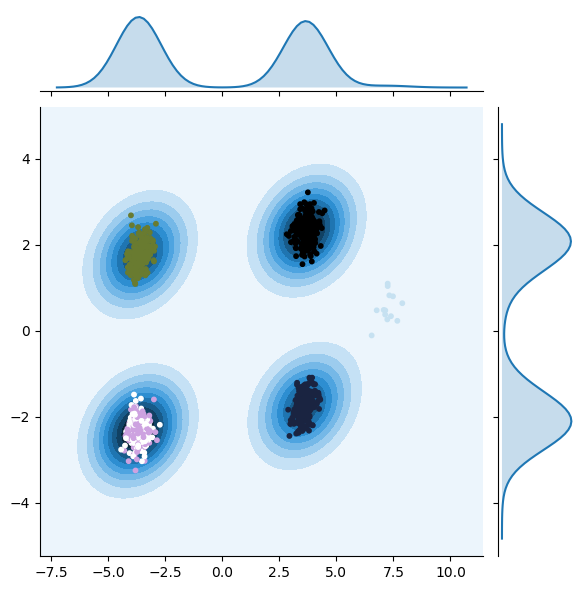
\includegraphics[width=0.9\linewidth]{articles/icf/figures/23000_kde_dh.png}}
\end{subfigure}
\centering
\begin{subfigure}{.45\textwidth}
{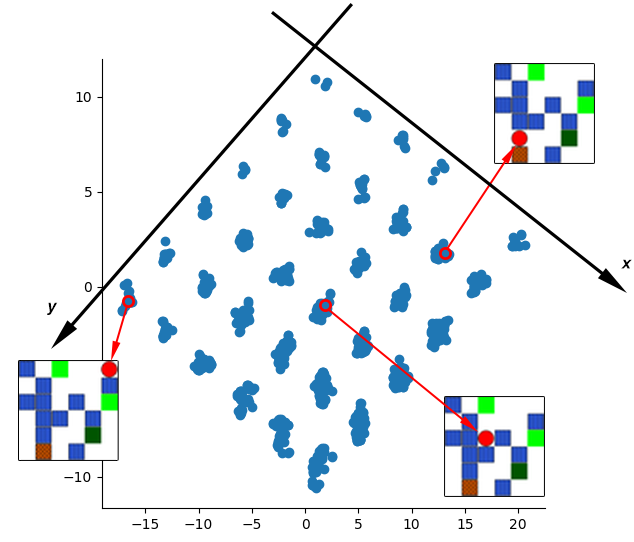
\includegraphics[width=0.9\linewidth]{articles/icf/figures/disentangle-kdeh.png}} %
\end{subfigure}

\caption{(a) Sampling of $1000$ variations $h' - h$ and its kernel density estimation encountered when sampling random controllable factors $\phi$. We observe that our algorithm disentangles these representations on $4$ main modes, each corresponding to the action that was actually taken by the agent.\protect\footnotemark
\, (b) The disentangled structure in the latent space. The $x$ and $y$ axis are disentangled such that we can recover the $x$ and $y$ position of the agent in any observation $s$ simply by looking at its latent encoding $h = f(s)$. The missing point on this grid is the only position the agent cannot reach as it lies on an orange block.}
\label{fig:dis_space}
\end{figure}

\footnotetext{pink and white for \texttt{up}, light blue for \texttt{down+left}, green for \texttt{right}, purple black \texttt{down} and night blue for \texttt{left}.}

After jointly training the reconstruction and selectivity losses, our algorithm disentangles four directed factors of variations as seen in Figure~\ref{fig:dis_space}: $\pm x$-position and $\pm y$-position of the agent. For visualization purposes we chose the bottleneck of the autoencoder to be of size $K = 2$.
To complicate the disentanglement task, we added the redundant action \texttt{up} as well as the action \texttt{down+left} in this experiment.

The disentanglement appears clearly as the latent features corresponding to the $x$ and $y$ position are orthogonal in the latent space. Moreover, we notice that our algorithm assigns both actions \texttt{up} (white and pink dots in Figure~\ref{fig:dis_space}.a) to the same feature. It also does not create a significant mode for the feature corresponding to the action \texttt{down+left} (light blue dots in Figure~\ref{fig:dis_space}.a) as this feature is already explained by features \texttt{down} and \texttt{left}.



\subsection{Towards planning and policy inference}
\label{sec:exp-mb-ppi}

This disentangled structure could be used to address many challenging issues in reinforcement learning. We give two examples in figure~\ref{fig:prediction_recovering}: 
\begin{itemize}
\item Model-based predictions: Given an initial state, $s_0$, and an action sequence $a_{\{0:T-1\}}$, %
we want to predict the resulting state $s_T$.

\item A simplified deterministic policy inference problem: Given an initial state $s_{start}$ and a terminal state $s_{goal}$, we aim to find a suitable action sequence $a_{\{0:T-1\}}$ such that $s_{goal}$ can be reached from $s_{start}$ by following it.
\end{itemize}
Because of the $tanh$ activation on the last layer of $\phi(h, z)$, the different factors of variation $dh = h' - h$ are placed on the vertices of a hypercube of dimension $K$, and we can think of the the policy inference problem as finding a path in that simpler space, where the starting point is $h_{start}$ and the goal is $h_{goal}$. We believe this could prove to be a much easier problem to solve.

\begin{figure}[t]
\centering
\begin{subfigure}{.45\textwidth}
\centering
{\scalebox{.6}{
\begin{tikzpicture}
\node[inner sep=0pt] (im0) at (0,0)
    {\fbox{
\includegraphics[width=.25\textwidth]{articles/icf/figures/im0_good.png}}};
\node[inner sep=0pt] (im1) at (5,0)
    {\fbox{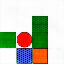
\includegraphics[width=.25\textwidth]{articles/icf/figures/im1_good.png}}};


\node[] (ht) at (0,-4) {$\underbrace{h}_{(0.4,\ 13.1)}$};
\node[] (ht1) at (7,-4) {$\underbrace{\hat{h'}}_{(-4.6,\ -1.9)} = h + \underbrace{dh_{{\color{right} {\color{right} right}}}}_{(5,\ -5)} + \underbrace{2\cdot dh_{{\color{down} down}}}_{(-10,\ -10)}$}; 
    \draw[->,thick] (im0.south) -- (ht.north)
    node[midway,fill=white] {Encoder};
    \draw[->,thick] (5, -3.3) -- (im1.south)
    node[midway,fill=white] {Decoder};
    
    \draw[->,thick] (ht.east) -- (ht1.west);
    
\end{tikzpicture}}}
\end{subfigure}
\begin{subfigure}{.45\textwidth}
\centering
{\scalebox{.6}{
\begin{tikzpicture}
\node[inner sep=0pt] (im0) at (0,0)
    {\fbox{
\includegraphics[width=.25\textwidth]{articles/icf/figures/im_causal0_good.png}}};
\node[inner sep=0pt] (im1) at (5,0)
    {\fbox{
\includegraphics[width=.25\textwidth]{articles/icf/figures/im_causal1_good.png}}};


\node[] (ht) at (0,-3.5) {$\underbrace{h_1}_{(0.4,\ 13.1)}$};
\node[] (ht1) at (5,-3.5) {$\underbrace{h_2}_{(5.9,\ -11.6)}$}; 
\node[] (dh) at (2.5,-5) {$dh ={(5.5,\ -24.8)} \approx 2\cdot dh_{{\color{down} down}} + 3\cdot dh_{{\color{right} right}}$};
    \draw[->,thick] (im0.south) -- (ht.north)
    node[midway,fill=white] {Encoder};
    \draw[<-,thick] (ht1) -- (im1.south)
    node[midway,fill=white] {Encoder};
    
    \draw[->,thick] (ht.east) -- (dh.north);
     \draw[->,thick] (ht1.west) -- (dh.north);
    
\end{tikzpicture}}
} %
\end{subfigure}
\caption{(left) Predicting the effect of a cause on Mazebase. The leftmost image is the visual input of the environment, where the agent is the round circle, and the switch states are represented by shades of green. After the training, we are able to distinguish one cluster per $dh$ (Figure \ref{fig:dis_space}), that is to say per variation obtained after performing an action, independently from the position $h$. Therefore, we are able to move the agent just by adding the corresponding $dh$ to our latent representation $h$. The second image is just the reconstruction obtained by feeding the resulting $h'$ into the decoder. (right) Given a starting state and a goal state, we are able to decompose the difference of the two representations $dh$ into a (non-directed) sequence of movements.}
\label{fig:prediction_recovering}
\end{figure}


However, this disentangled representation alone cannot solve completely these two issues in an arbitrary environment. Indeed, the only factors we are able to disentangle are the factors directly \textit{controllable} by the agent, thus, we are not able to account for the ambient dynamics or other agents' influence.



\subsection{Multistep embedding of policies}
In this experiment, $\phi$ are embeddings of $3$-steps policies $\pi_\phi$. We add a model-based loss $\mathcal{L}_{MB}=||h_{t+3} - T_\theta(h_t, \phi)||^2$ defined only in the latent space, and jointly train a decoder alongside with the encoder. Notice that we never train our model-based cost at pixel level.
While we currently suffer from mode collapsing of some factors of variations, we show that we are successfully able to do predictions in latent space, reconstruct the latent prediction with the decoder, and that our factor space disentangles several types of variations.

\begin{figure}
\centering
\begin{subfigure}{.45\textwidth}
{{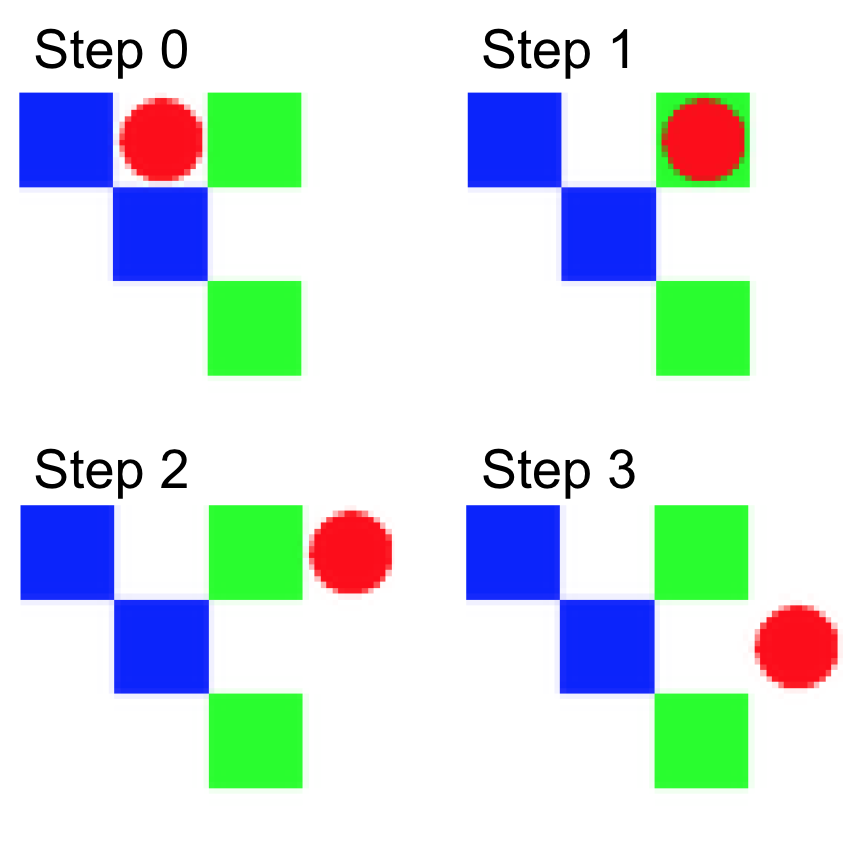
\includegraphics[width=.65\linewidth]{articles/icf/figures/square_traj.png}}} %
\end{subfigure}
\begin{subfigure}{.45\textwidth}
{{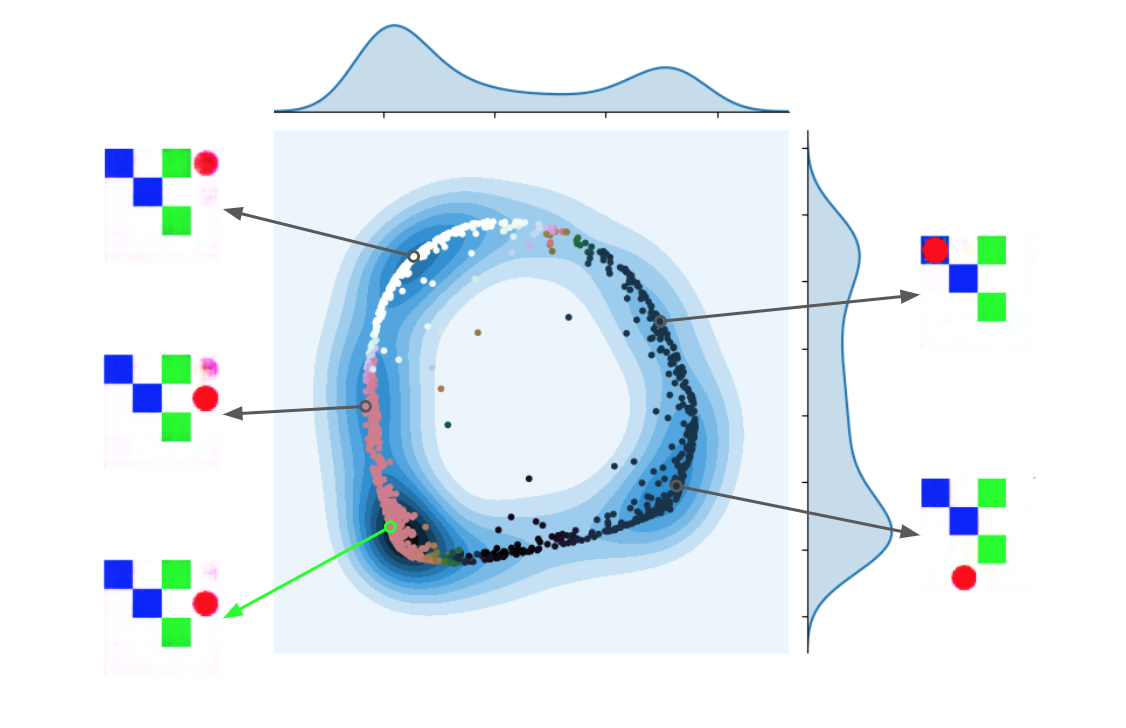
\includegraphics[width=.90\linewidth]{articles/icf/figures/phi_space.png}}}
\end{subfigure}

\caption{(a) The actual 3-step trajectory done by the agent. (b) PCA view of the space $\phi(h_0, z), z \sim \mathcal{N}(0,1)$. Each arrow points to the reconstruction of the prediction $T_\theta(h_0, \phi)$ made by different $\phi$. The $\phi$ at the start of the green arrow is the one used by the policy in (a). Notice how its prediction accurately predicts the actual final state.}
\end{figure}





\section{Conclusion, success and limitations}
Pushing representations to model independently controllable features currently yields some encouraging success. Visualizing our features clearly shows the different controllable aspects of simple environments, yet, our learning algorithm is unstable. What seems to be the strength of our approach could also be its weakness, as the independence prior forces a very strict separation of concerns in the learned representation, and should maybe be relaxed.

Some sources of instability also seem to slow our progress: learning a conditional distribution on controllable aspects that often collapses to fewer modes than desired, learning stochastic policies that often optimistically converge to a single action, tuning many hyperparameters due to the multiple parts of our model. Nonetheless, we are hopeful in the steps that we are now taking. Disentangling happens, but understanding our optimization process as well as our current objective function will be key to further progress. 

\chapter{Probabilistic Planning with Sequential Monte Carlo Methods}
\label{chapter:smcp}
\section*{Article details}


Thomas, V.*, Piché, A.*, , Ibrahim, C., Bengio, Y. and Pal, C. ``Probabilistic Planning with Sequential Monte Carlo methods''. In \emph{International Conference on Learning Representations (ICLR) 2019}.

This work was done jointly with Alexandre Pich\'{e} during the summer 2018 at Mila and ElementAI and was presented at ICLR 2019. 
\section*{Foreword}
The original intuition was that it should be possible to have a tree search planning algorithm where interesting (\emph{i.e} might get high return) branches were reinforced and less interesting branches cut off. Using control as inference was a natural way to associate the return a branch might get to the probability it would have to be reinforced or cut.

To the best of our knowledge, there is only one article that framed planning as an inference problem~\citep{attias2003planning} and it was in a very specific setting with strong assumptions.
We realized that our idea was intimately linked with sequential Monte Carlo methods and that our algorithm could be framed as an instance of a particle filter.
In control theory, there is a duality between estimating the current state and controlling the dynamics to the desired goal. While particle filters are typically used for estimation, here, within the context of control as inference, we are able to design a particle filter algorithm for control.



\section*{Impact since publication}
This paper already has some citations and follow-up works using our formulation of planning as inference and our algorithm~\citep{wang2019dual, lioutas2022critic}. An evalution paper, \citep{byravan22eval}, found that SMCP performed favorably compared to CEM, both on performance and computational complexity
        ``[...] on the \textbf{harder GTTP tasks SMC slightly outperforms CEM}. We use SMC throughout the paper as it makes better use of the proposal [distribution] compared to CEM 
        [...]
        \textbf{CEM uses a significantly larger computational budget than our SMC planner} which is non-iterative; in spite of this SMC is still quite competitive with CEM across all tasks [...]''

A book~\citep{belousov2021reinforcement} cites SMCP as a promising direction for planning: ''Recent research in probabilistic dynamic models and planning
with sequential Monte Carlo methods viewing control as an inference problem demonstrate the advantages of probabilistic plan
ning in MPC and may be \textbf{one of the most promising directions}[to improve MPC in a black box environment].''


\section*{Personal contribution}
\begin{itemize}
    \item Major contribution on the theoretical understanding of the method. Made the link with the two-filter formula~\citep{bresler1986two} and smoothing/forward-backward algorithms
    \item Determined the expression for the update (maximum entropy advantage) and wrote the proofs in the appendix
    \item Designed and performed the toy experiment~\Cref{fig:toy_sis} and \Cref{fig:toy_sir}
    \item Made \Cref{fig:hmm}, \Cref{fig:tree} and \Cref{fig:alphabeta}
    \item Writing of the paper alongside with Alexandre
\end{itemize}

\newpage
\begin{abstract}
In this work, we propose  a novel formulation of planning which views it as a probabilistic inference problem over future optimal trajectories. This enables us to use sampling methods, and thus, tackle planning in continuous %
domains using a fixed computational budget.  We design a new algorithm, Sequential Monte Carlo Planning, by leveraging classical methods in Sequential Monte Carlo and Bayesian smoothing in the context of \textit{control as inference}.  %
Furthermore, we show that Sequential Monte Carlo Planning can capture multimodal policies and can quickly learn continuous control tasks. %
\end{abstract}

\section{Introduction}

To exhibit intelligent behaviour machine learning agents must be able to learn quickly, predict the consequences of their actions, and explain how they will react in a given situation. These abilities are best achieved when the agent efficiently uses a model of the world to plan future actions. To date, planning algorithms have yielded very impressive results. For instance, Alpha Go~\citep{silver2017mastering} relied on Monte Carlo Tree Search (MCTS)~\citep{kearns2002sparse} to achieve super human performances. Cross entropy methods (CEM) \citep{rubinstein2004unified} have enabled robots to perform complex nonprehensile manipulations \citep{finn2017deep} and algorithms to play successfully Tetris \citep{szita2006learning}. In addition, iterative linear quadratic regulator (iLQR) \citep{kalman1960contributions, kalman1964linear, todorov2005generalized} enabled humanoid robots tasks to get up from an arbitrary seated pose \citep{tassa2012synthesis}. 


Despite these successes, these algorithms make strong underlying assumptions about the environment.
First, MCTS requires a discrete setting, limiting most of its successes to discrete games with known dynamics.
Second, CEM assumes the distribution over future trajectories to be Gaussian, i.e. unimodal. Third, iLQR assumes that the dynamics are locally linear-Gaussian, which is a strong assumption on the dynamics and would also assume the distribution over future optimal trajectories to be Gaussian. For these reasons, planning remains an open problem in environments with continuous actions and complex dynamics. In this paper, we address the limitations of the aforementioned planning algorithms by creating a more general view of planning that can leverage advances in deep learning (DL) and probabilistic inference methods. This allows us to approximate arbitrary complicated distributions over trajectories with non-linear dynamics.


We frame planning as density estimation problem over optimal future trajectories in the context of \textit{control as inference} \citep{dayan1997using, toussaint2006probabilistic, toussaint2009robot, rawlik2010approximate, rawlik2012stochastic, ziebart2010modeling, levine2013variational}.  This perspective allows us to make use of tools from the inference research community and, as previously mentioned, model any distribution over future trajectories. The planning distribution is complex since trajectories consist of an intertwined sequence of states and actions. Sequential Monte Carlo (SMC) \citep{stewart1992use, gordon1993novel, kitagawa1996monte} methods are flexible and efficient to model such a distribution by sequentially drawing from a simpler proposal distribution.
From the SMC perspective, the policy can be seen as the proposal and a learned model of the world as the propagation distribution. This provides a natural way to combine model-free and model-based RL.


\textbf{Contribution.} We depict the problem of planning as one of density estimation that can be estimated using SMC methods. We introduce a novel planning strategy based on the SMC class of algorithms, in which we treat the policy as the proposed distribution to be learned. We investigate how our method empirically compares with existing model-based methods and a strong model-free baseline on the standard benchmark Mujoco~\citep{todorov2012mujoco}. 


\section{Background}
\subsection{Control as inference}
\label{sec:control_as_inference}

We consider the general case of a Markov Decision Process (MDP) $\{\gS, \gA, \penv, r, \gamma, \mu\}$ where $\gS$ and $\gA$ represent the state and action spaces respectively. We use the letters $s$ and $a$ to denote states and actions, which we consider to be continuous vectors. Further notations include: $\penv(s' |s, a)$ as the state transition probability of the environment, $r(s, a)$ %
as the reward function, and $\gamma \in [0, 1)$ as the discount factor. $\mu$ denotes the probability distribution over initial states.

This work focuses on an episodic formulation, with a fixed end-time of $T$. We define a trajectory as a sequence of state-action pairs $\traj_{t:T}=\{(s_t,a_t), \ldots,(s_T, a_T) \}$, and we use the notation $\pi$ for a policy which represents a distribution over actions conditioned on a state. Here $\pi$ is parametrized by a neural network with parameters $\parampol$. The notation %
$q_\parampol(\traj_{1:T}) = \mu(s_1) \prod_{t \geq 1}^{T-1} \penv(s_{t+1}|s_t, a_t) \prod_{t \geq 1}^{T} \pi_\parampol(a_t|s_t)$
denotes the probability of a trajectory $\traj_{1:T}$ under policy $\pi_\parampol$. 


\setlength{\wrapoverhang}{\marginparwidth}
\addtolength{\wrapoverhang}{\marginparsep}
\begin{wrapfigure}{r}[-1mm]{.5\linewidth}%
\centering
\resizebox{.95\linewidth}{!}{
\begin{tikzpicture}
\tikzstyle{main}=[circle, minimum size = 5mm, thick, draw =black!80, node distance = 7mm]
\tikzstyle{connect}=[-latex, thick]
\tikzstyle{box}=[rectangle, draw=black!100]
  \node[box,draw=white!100] (Latent) {\textbf{Latent}};
  \node[main] (a1) [right=of Latent] {$\va_1$};
  \node[main] (s1) [below=of a1] {$\vs_1$};
  \node[draw,thick, rounded corners, fit=(s1) (a1)] (L1) {};
  \node[main] (a2) [right=of a1] {$\va_2$};
  \node[main] (s2) [below=of a2] {$\vs_2$};
  \node[draw,thick, rounded corners, fit=(s2) (a2)] (L2) {};
  \node[main] (a3) [right=of a2] {$\va_3$};
  \node[main] (s3) [below=of a3] {$\vs_3$};
  \node[draw,thick, rounded corners, fit=(s3) (a3)] (L3) {};
  \node[main] (at) [right=of a3] {$\va_t$};
  \node[main] (st) [below=of at] {$\vs_t$};
  \node[draw,thick, rounded corners, fit=(st) (at)] (Lt) {};
  
  
  \node[box,draw=white!100] (Observed) [above=of Latent] {\textbf{Observed}};
  \node[main,fill=black!10] (O1) [right=of Observed,above=of L1] {$\gO_1$};
  \node[main,fill=black!10] (O2) [right=of O1,above=of L2] {$\gO_2$};
  \node[main,fill=black!10] (O3) [right=of O2,above=of L3] {$\gO_3$};
  \node[main,fill=black!10] (Ot) [right=of O3,above=of Lt] {$\gO_t$};

  \path (L3) -- node[auto=false]{\ldots} (Lt);
  \path (a1) edge [connect] (O1)
        (s1) edge [connect, bend right=45] (O1)
        (s1) edge [connect] (s2)
        (a1) edge [connect] (s2);
    \path (a2) edge [connect] (O2)
        (s2) edge [connect, bend right=45] (O2)
        (s2) edge [connect] (s3)
        (a2) edge [connect] (s3);
  \path (a3) edge [connect] (O3)
        (s3) edge [connect, bend right=45] (O3);
  \path (at) edge [connect] (Ot)
        (st) edge [connect, bend right=45] (Ot);
  \path (L3) -- node[auto=false]{\ldots} (Lt);

  \draw[dashed]  [below=of L1,above=of O1];
\end{tikzpicture}
}
\caption{$\mathcal{O}_t$ is an observed \textit{optimality} variable with probability $p(\mathcal{O}_t|s_t, a_t) = \exp(r(s_t,a_t))$. $\traj_t = (s_t, a_t)$ are the state-action pair variables considered here as latent.}
\label{fig:graphical_model}
\end{wrapfigure}

Traditionally, in reinforcement learning (RL) problems, the goal is to find the optimal policy that maximizes the expected return $\mathbb{E}_{\qpol}[\sum_{t=1}^T \gamma^t r_t]$. 
However, it is useful to frame RL as an inference problem within a probabilistic graphical framework \citep{rawlik2012stochastic, toussaint2006probabilistic, levine2018reinforcement}. First, we introduce an auxiliary binary random variable $\gO_t$ denoting the ``optimality`` of a pair $(s_t, a_t)$ at time $t$ and define its probability\footnote{as in~\cite{levine2018reinforcement}, if the rewards are bounded above, we can always remove a constant so that the probability is well defined.} as $p(\gO_{t}=1|s_t, a_t) = \exp(r(s_t, a_t))$. $\gO$ is a convenience variable only here for the sake of modeling. By considering the variables $(s_t, a_t)$ as latent and $\gO_t$ as observed, we can construct a Hidden Markov Model (HMM) as depicted in figure \ref{fig:graphical_model}.
Notice that the link $s \rightarrow a$ is not present in figure~\ref{fig:graphical_model} as the dependency of the optimal action on the state depends on the future observations. In this graphical model, the optimal policy is expressed as $p(a_t | s_t, \gO_{t:T})$.


The posterior probability of this graphical model can be written as\footnote{Notice that in the rest of the paper, we will abusively remove the product of the action priors $\prod_{t=1}^{T} p(a_t) = \exp\big(\sum_{t=1}^{T}\log p(a_t)\big)$ from the joint as in~\cite{levine2018reinforcement}. We typically consider this term either constant or already included in the reward function. See Appendix~\ref{app:action_prior} for details.}: 
\begin{equation}
\label{eq:posterior_target}
p(\traj_{1:T} | \gO_{1:T}) \propto p(\traj_{1:T}, \gO_{1:T}) = \mu(s_1) \prod_{t=1}^{T-1} \penv(s_{t+1}|a_t, s_t) \exp\big(\sum_{t=1}^{T} r(s_t, a_t) + \textcolor{gray}{\log p(a_t) } \big).
\end{equation}


It appears clearly that finding optimal trajectories is equivalent to finding plausible trajectories yielding a high return.



Many \textit{control as inference} methods can be seen as approximating the density by optimizing its variational lower bound: $\log p(\mathcal{O}_{1:T}) \geq \mathbb{E}_{\traj_{1:T}\sim q_\theta} [\sum_{t=1}^T r(s_t, a_t) - \log \pi_\theta(a_t|s_t) ]$  \citep{rawlik2012stochastic, toussaint2009robot}. Instead of directly differentiating the variational lower bound for the whole trajectory, it is possible to take a message passing approach such as the one used in Soft Actor-Critic (SAC) \citep{haarnoja2018soft} and directly estimate the optimal policy $p(a_t | s_t, \gO_{t:T})$ using the backward message, i.e a soft $Q$ function instead of the Monte Carlo return.


\subsection{Sequential Monte Carlo methods}
\label{sec:smc}




Since distributions over trajectories are complex, it is often difficult or impossible to directly draw samples from them. Fortunately in statistics, there are successful  strategies for drawing samples from complex sequential distributions, such as SMC methods.%

For simplicity, in the remainder of this section we will overload the notation and refer to the target distribution as $p(\traj)$ and the proposal distribution as $q(\traj)$.
We wish to draw samples from $p$ but we only know its unnormalized density. We will use the proposal $q$ to draw samples and estimate $p$.
In the next section, we will define the distributions $p$ and $q$ in the context of planning.  

\paragraph{Importance sampling (IS):} When $\traj$ can be efficiently sampled from another simpler distribution $q$ i.e. the proposal distribution, we can estimate the likelihood of any point $\traj$ under $p$ straightforwardly by computing the \emph{unnormalized importance sampling weights} $w(\traj) \propto \tfrac{p(\traj)}{q(\traj)}$ and using the identity $p(\traj) = \bar{w}(\traj) q(\traj)$ where $\bar{w}(\traj) = \tfrac{w(\traj)}{\int w(\traj) q(\traj) d \traj}$ is defined as the \emph{normalized importance sampling weights}. In practice, one draws $N$ samples from $q$: $\{\traj^{(n)}\}_{n=1}^N \sim q$; these are referred to as \emph{particles}. The set of particles $\{\traj^{(n)}\}_{n=1}^N$ associated with their weights $\{{w}^{(n)} \}_{n=1}^N$ are simulations of samples from $p$. That is, we approximate the density $p$ with a weighted sum of diracs from samples of $q$: $$p(\traj) \approx \sum_{n=1}^N \bar{w}^{(n)} \delta_{\traj^{(n)}} (\traj), \, \text{with}\, \traj^{(n)}\, \text{sampled from}\, q$$ where $\delta_{\traj_0}(\traj)$ denotes the Dirac delta mass located as $\traj_0$.

\paragraph{Sequential Importance Sampling (SIS):} When our problem is sequential in nature $\traj = \traj_{1:T}$, 
sampling $\traj_{1:T}$ at once can be a challenging or even intractable task.
By exploiting the sequential structure, the unnormalized weights can be updated iteratively in an efficient manner: 
$
w_t(\traj_{1:t}) %
= w_{t-1}(\traj_{1:t-1}) \frac{p(\traj_t|\traj_{1:t-1})}{ q(\traj_t|\traj_{1:t-1})}$. We call this the \textbf{update step}. 
This enables us to sample sequentially $\traj_t \sim q(\traj_t | \traj_{1:t-1})$ to finally obtain the set of particles $\{\traj^{(n)}_{1:T}\}$ and their weights $\{{w}^{(n)}_T \}$ linearly in the horizon $T$.

\paragraph{Sequential Importance Resampling (SIR):}  When the horizon $T$ is long, samples from $q$ usually have a low likelihood under $p$, and thus the quality of our approximation decreases exponentially with $T$. More concretely, the unnormalized weights $w^{(n)}_t$ converge to $0$ with $t \rightarrow \infty$. This usually causes the normalized weight distribution to degenerate, with one weight having a mass of $1$ and the others a mass of $0$. This phenomenon is known as \emph{weight impoverishment}.

One way to address weight impoverishment is to add a \textbf{resampling step} where each particle is stochastically resampled to higher likelihood regions at each time step. 
This can typically reduce the variance of the estimation from growing \emph{exponentially} with $t$ to growing \emph{linearly}. 




















\section{Sequential Monte Carlo Planning}
\label{sec:smcp}
In the context of \textit{control as inference}, it is natural to see planning as the act of approximating a distribution of optimal future trajectories via simulation. In order to plan, an agent must possess a model of the world that can accurately capture the consequences of its actions. In cases where multiple trajectories have the potential of being optimal, the agent must rationally partition its computational resources to explore each possibility. Given finite time, the agent must limit its planning to a finite horizon $h$. We, therefore, define \textit{planning} as the act of approximating the optimal distribution over trajectories of length \textit{h}. In the control-as-inference framework, this distribution is naturally expressed as $p(a_1, s_2, \dots s_h, a_h | \gO_{1:T}, s_1)$, where $s_1$ represents our current state. 


\subsection{Planning and Bayesian smoothing}

As we consider the current state $s_1$ given, it is equivalent and convenient to focus on the planning distribution with horizon $h$: $p(\traj_{1:h}|\gO_{1:T})$. Bayesian smoothing is an approach to the problem of estimating the distribution of a latent variable conditioned on all past and future observations. One method to perform smoothing is to decompose the posterior with the \textit{two-filter formula}~\citep{bresler1986two, kitagawa1994two}:


\begin{align}
\label{eq:forwardbackward}
    {p(\traj_{1:h} | \gO_{1:T})} & \propto \mathunderline{alpha}{p(\traj_{1:h}|\gO_{1:h})} \cdot \mathunderline{beta}{p(\gO_{h+1:T}|\traj_{h})}
\end{align}





\noindent This corresponds to a forward-backward messages factorization in a Hidden Markov Model as depicted in Figure~\ref{fig:hmm}. We broadly underline in orange forward variables and in blue backward variables in the rest of this section.




\setlength{\wrapoverhang}{\marginparwidth}
\addtolength{\wrapoverhang}{\marginparsep}
\begin{wrapfigure}{r}[-1mm]{.5\linewidth}%
\centering
\resizebox{.95\linewidth}{!}{
  
  

    
        

\begin{tikzpicture}
\tikzstyle{main}=[circle, minimum size = 12mm, thick, draw =black!80, node distance = 8mm]
\tikzstyle{connect}=[-latex, thick]
\tikzstyle{connect}=[-latex, thick]
\tikzstyle{box}=[rectangle, draw=black!100]
  \node[main, fill=alpha] (x1) {$\traj_1$};
  
  \node[main, fill=alpha] (xtm1) [right=of x1] {$\traj_{h-1}$};
  \node[main, fill=alpha] (xt) [right=of xtm1] {$\traj_h$};
  \node[main, fill=beta] (xtp1) [right=of xt] {$\traj_{h+1}$};
  \node[main, fill=beta] (xT) [right=of xtp1] {$\traj_{T}$};
  
  
  \node[main, fill=alpha] (O1) [right=of Observed,above=of x1] {$\gO_1$};
  \node[main, fill=alpha] (Otm1) [right=of O1,above=of xtm1] {$\gO_{h-1}$};
  \node[main, fill=alpha] (Ot) [right=of Otm1,above=of xt] {$\gO_h$};
  \node[main,fill=beta] (Otp1) [right=of Ot,above=of xtp1] {$\gO_{h+1}$};
  \node[main,fill=beta] (OT) [right=of Otp1,above=of xT] {$\gO_T$};

  \path (x1) edge [connect] (O1);
  \path (x1) edge [connect, dashed] (xtm1);
  \path (xtm1) edge [connect] (Otm1)
        (xtm1) edge [connect] (xt)
        ;
    \path (xt) edge [connect] (Ot)
        (xt) edge [connect] (xtp1)
        ;    
    \path (xtp1) edge [connect] (Otp1);
        ;  
    \path (xtp1) edge [connect, dashed] (xT);
    \path (xT) edge [connect] (OT);
        ;    
    
        
  \path (xt) edge [connect] (Ot);

  \draw[dashed]  [below=of L1,above=of O1];
  \draw[ultra thick,->] (0,-1) -- (4.5,-1) node[anchor=north] {};
  \draw[ultra thick,->] (8,-1) -- (5.5,-1) node[anchor=north] {};

    \node[] (alpha) at (2.5, -1.5) {$p(\traj_{1:h}|\gO_{1:h})$};
  \node[] (alpha) at (6.5, -1.5) {$p(\gO_{h+1:T}|\traj_{h})$};
\end{tikzpicture}

}
\caption{Factorization of the HMM into  {\color{alpha} forward} (orange) and {\color{beta} backward} (blue) messages. Estimating the forward message is filtering, estimating the value of the latent knowing all the observations is smoothing.}
\label{fig:alphabeta}
\end{wrapfigure}

\textbf{Filtering} is the task of estimating $p(\traj_{1:t} | \gO_{1:t})$: the probability of a latent variable conditioned on all past observations. In contrast, \textbf{smoothing} estimates $p(\traj_{1:t} | \gO_{1:T})$: the density of a latent variable conditioned on all the past and future measurements. 

In the belief propagation algorithm for HMMs, these probabilities correspond to the forward message $\alpha_{h}(\traj_{h}) = p(\traj_{1:h}|\gO_{1:h})$ and backward message $\beta_{h}(\traj_{h}) = {p(\gO_{h+1:T}|\traj_{h})}$ , both of which are computed recursively.
While in discrete spaces these forward and backward messages can be estimated using the sum-product algorithm, its complexity scales with the square of the space dimension making it unsuitable for continuous tasks. We will now devise efficient strategies for estimating reliably the full posterior using the SMC methods covered in section~\ref{sec:smc}.



\subsection{The Backward Message and the Value Function}
The backward message $p(\gO_{h+1:T}| \traj_h)$ can be understood as the answer to: \textit{What is the probability of following an optimal trajectory from the next time step on until the end of the episode, given my current state?}. %
Importantly, this term is closely related to the notion of \textit{value function} in RL. Indeed, in the control-as-inference framework, the  state- and action-value functions are defined as $V(s_h) \triangleq \log p(\gO_{h:T}|s_h)$ and $Q(s_h, a_h) \triangleq \log p(\gO_{h:T}|s_h, a_h)$ respectively. They are solutions of a soft-Bellman equation that differs a little from the traditional Bellman equation~\citep{o2016combining, nachum2017bridging, schulman2017equivalence, abdolmaleki2018maximum}. 
A more in depth explanation can be found in~\citep{levine2018reinforcement}. We can show subsequently that: %
\begin{align}
p(\gO_{h+1:T}|\traj_{h}) =\mathunderline{beta}{ \E_{s_{h+1} | \traj_h }\left[\exp\big(V(s_{h+1})\big)\right]}
\end{align}

\noindent Full details can be found in Appendix~\ref{app:backward_message}. Estimating the backward message is then equivalent to learning a value function.  
This value function as defined here is the same one used in Maximum Entropy RL~\citep{ziebart2010modeling}.


\subsection{Sequential Weight Update}
Using the results of the previous subsections we can now derive the full update of the sequential importance sampling weights. To be consistent with the terminology of section~\ref{sec:smc}, we call $p(\traj_{1:h} | \gO_{1:T})$ the target distribution and $q_\parampol(\traj_{1:h})$ the proposal distribution. The sequential weight update formula is in our case:

\begin{align}
w_t 
&= w_{t-1} \cdot \frac{p(\traj_t |\traj_{1:t-1}, \gO_{1:T})}{q_\parampol(\traj_t | \traj_{1:t-1})} \nonumber\\
&\propto w_{t-1}   \frac{1}{ q_\parampol(\traj_t | \traj_{1:t-1})} \frac{\mathunderline{alpha}{p(\traj_{1:t} | \gO_{1:t})}}{ \mathunderline{alpha}{p(\traj_{1:t-1} | \gO_{1:t-1})}} \frac{ \mathunderline{beta}{p(\gO_{t+1:T} | \traj_{t})}}{ \mathunderline{beta}{p(\gO_{t:T} | \traj_{t-1})}}   \nonumber\\
&\propto w_{t-1} \cdot \frac{\penv(s_t | s_{t-1}, a_{t-1})}{\pmodel(s_t | s_{t-1}, a_{t-1})} \cdot \E_{s_{t+1} | s_t, a_t} [ \exp \big( A(s_t, a_t, s_{t+1}) \big)] \nonumber
\end{align}
Where \begin{equation}
\label{eq:maxent_advantage}
A(s_t, a_t, s_{t+1}) = r_t -  \log \pi_\parampol(a_t | s_t) + V(s_{t+1}) - \log \E_{s_{t} | s_{t-1}, a_{t-1}} [ \exp \big( V(s_{t}) \big)]
\end{equation}
is akin to a maximum entropy advantage function. The change in weight can be interpreted as sequentially correcting our expectation of the return of a trajectory.


\noindent The full derivation is available in Appendix~\ref{app:rec_weights}. Our algorithm is similar to the Auxiliary Particle Filter \citep{pitt1999filtering} which uses a one look ahead simulation step to update the weights.
 Note that in practice we do not have access to the ratio $\frac{\penv(s_t | s_{t-1}, a_{t-1})}{\pmodel(s_t | s_{t-1}, a_{t-1})}$, as it would be equivalent to having access to a perfect model of the world otherwise. Therefore, we will use the simplified weight update:
 
 $$w_t \propto w_{t-1} \cdot \E_{s_{t+1} | s_t, a_t} [ \exp \big( A(s_t, a_t, s_{t+1}) \big)]$$
 
 by assuming our model of the environment is perfect to obtain this slightly simplified form.
 
 This assumption is implicitly made by most planning algorithms (LQR, CEM \dots): it entails that our plan is only as good as our model is. A typical way to mitigate this issue and be more robust to model errors is to re-plan at each time step; this technique is called Model Predictive Control (MPC) and is commonplace in control theory.


\subsection{Sequential Monte Carlo Planning Algorithm}

We can now use the computations of previous subsections to derive the full algorithm. We consider the root state of the planning to be the current state $s_t$. We aim at building a set of particles $\{\traj^{(n)}_{t:t+h}\}_{n=1}^N$  and their weights $\{w^{(n)}_{t+h} \}_{n=1}^N$ representative of the planning density $p(\traj_{t:t+h} | \gO_{1:T})$ over optimal trajectories. We use SAC~\citep{haarnoja2018soft} for the policy and value function, but any other Maximum Entropy policy can be used for the proposal distribution. Note that we used the value function estimated by SAC as a proxy the optimal one as it is usually done by actor critic methods.




\begin{algorithm}[H]
\caption{SMC Planning using SIR}
\label{alg:sir_planning}
\begin{algorithmic}[1]
\FOR{$t$ in $\{1,\ldots,T\}$}
\STATE $\{ s^{(n)}_t = s_t\}_{n=1}^N$
\STATE  $\{w^{(n)}_t =1\}_{n=1}^N$
\FOR{$i$ in $\{t,\ldots,t+h\}$}
\STATE \textit{// Update}
\STATE $\{a^{(n)}_{i} \sim \pi(a^{(n)}_{i}|s^{(n)}_{i})\}_{n=1}^N$
\STATE $\{s^{(n)}_{i+1}, r^{(n)}_{i} \sim \pmodel(\cdot | s^{(n)}_{i}, a^{(n)}_{i})\}_{n=1}^N$
\STATE $\{w_i^{(n)} \propto w^{(n)}_{i-1} \cdot \exp \big( A(s^{(n)}_{i}, a^{(n)}_{i}, s^{(n)}_{i+1}) \big) \}_{n=1}^N$
\STATE \textit{// Resampling}
\STATE $\{\traj^{(n)}_{1:i}\}_{n=1}^N \sim \text{Mult}(n; w_{i}^{(1)}, \ldots, w_{i}^{(N)})$
\STATE $\{w_i^{(n)} =1 \}_{n=1}^N$
\ENDFOR
 \STATE Sample $n \sim \text{Uniform}(1, N)$.
\STATE \textit{// Model Predictive Control}
\STATE Select $a_t$, first action of $\traj^{(n)}_{t:t+h}$
\STATE $s_{t+1}, r_t \sim p_{\text{env}}(\cdot|s_t, a_t)$
\STATE Add $(s_t, a_t, r_t, s_{t+1})$ to buffer $\mathcal{B}$
\STATE Update $\pi$, $V$ and $\pmodel$ with $\mathcal{B}$
\ENDFOR
\end{algorithmic}
\end{algorithm}

We summarize the proposed algorithm in Algorithm \ref{alg:sir_planning}. At each step, we sample from the proposal distribution or model-free agent (\textbf{line 6}) and use our learned model to sample the next state and reward (\textbf{line 7}). We then update the  weights (\textbf{line 8}). In practice we only use one sample to estimate the expectations, thus we may incur a small bias. The resampling step is then performed (\textbf{line 10-11}) by resampling the trajectories according to their  weight. After the planning horizon is reached, we sample one of our trajectories (\textbf{line 13}) and execute its first action into the environment (\textbf{line 15-16}). The observations $(s_t, a_t, r_t, s_{t+1})$ are then collected and added to a buffer (\textbf{line 17}) used to train the model as well as the policy and value function of the model-free agent. An alternative algorithm that does not use the resampling step (SIS) is highlighted in Algorithm \ref{alg:sis_planning} in Appendix~\ref{app:sis_algo}.

A schematic view of the algorithm can also be found on figure~\ref{fig:tree}.

\begin{figure}[h!]
\centering
\begin{subfigure}{.30\textwidth}
  \centering
  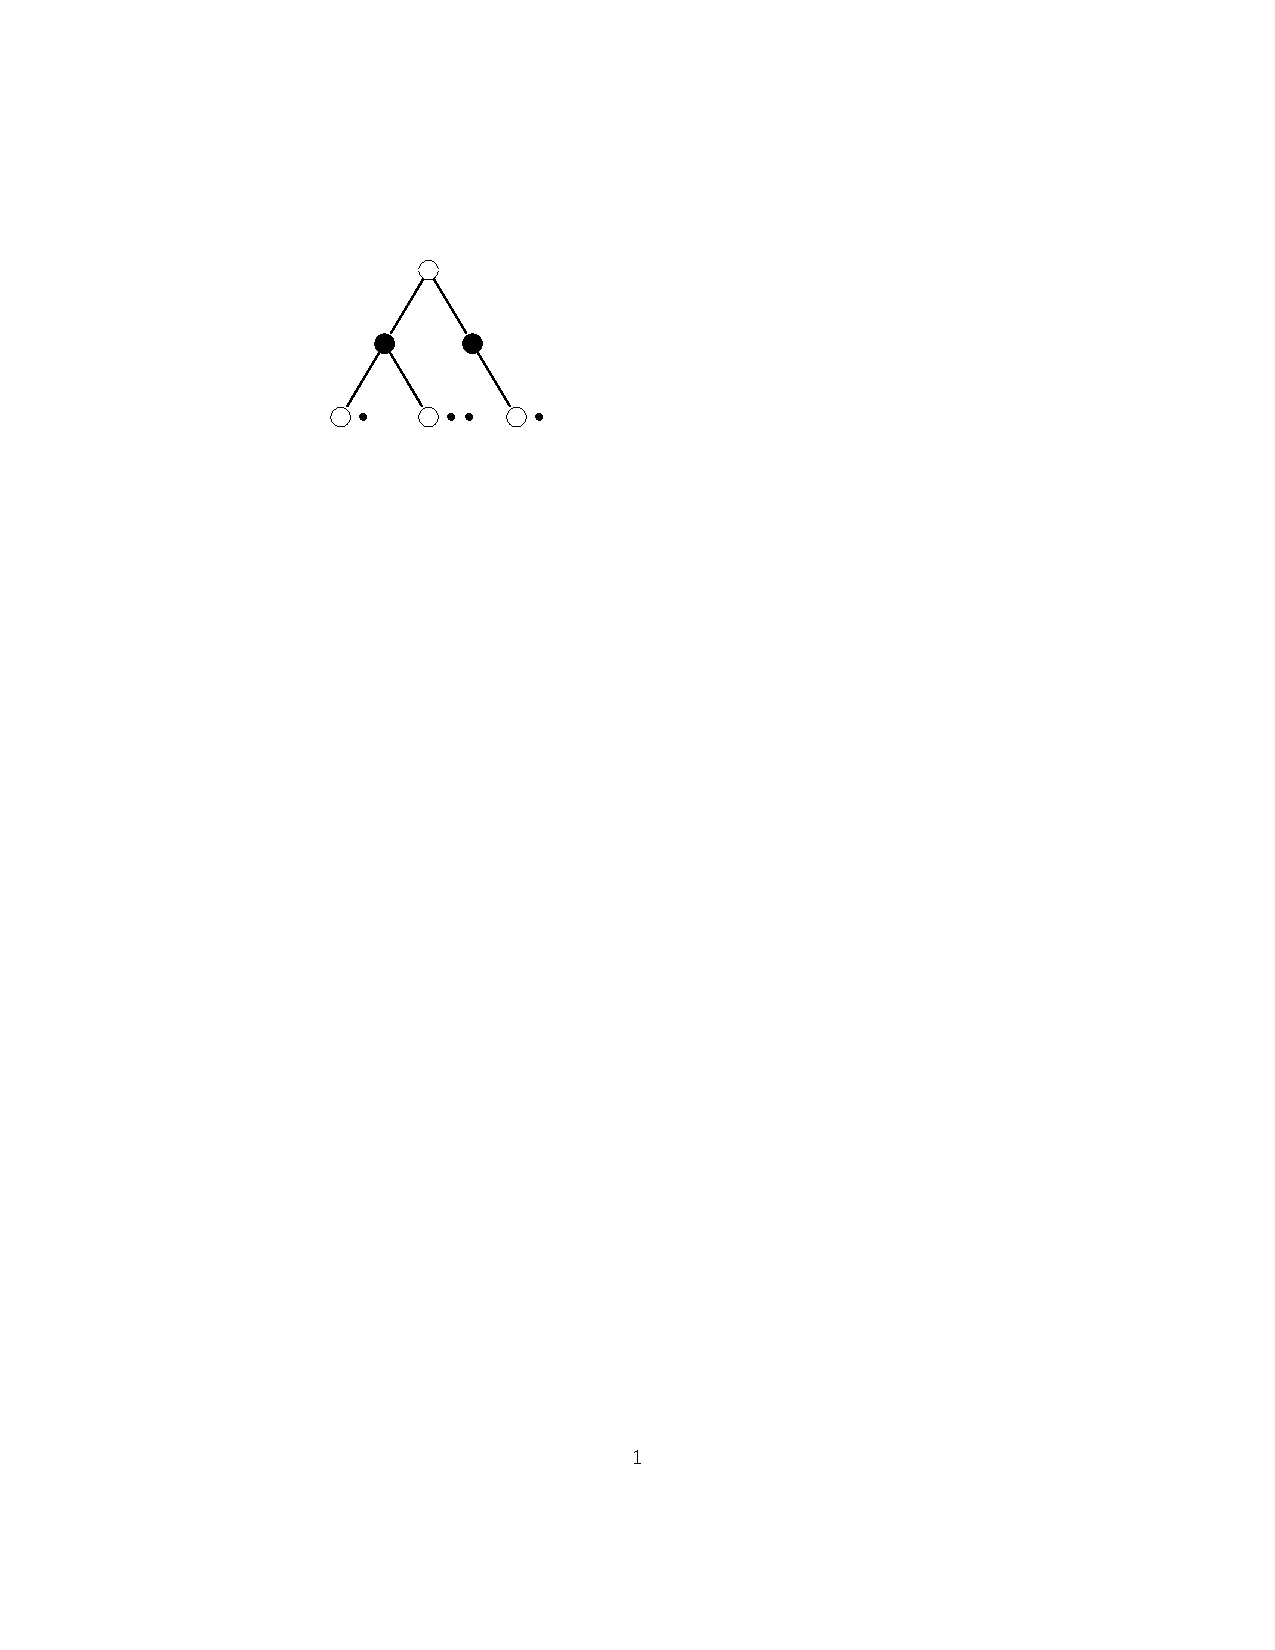
\includegraphics[width=0.7\linewidth, trim={5cm 17cm 12cm 4cm},clip]{articles/smcp/figures/main_ts1.pdf}
  \caption{\textbf{Configuration at time $t-1$:} we have the root white node $s_{t-1}$, the actions $a^{(n)}_{t-1}$ are black nodes and the leaf nodes are the $s^{(n)}_t$. We have one particle on the leftmost branch, two on the central branch and one on the rightmost branch. }
  \label{fig:sub1}
\end{subfigure}\hspace{.03\linewidth}
\begin{subfigure}{.30\textwidth}
  \centering
  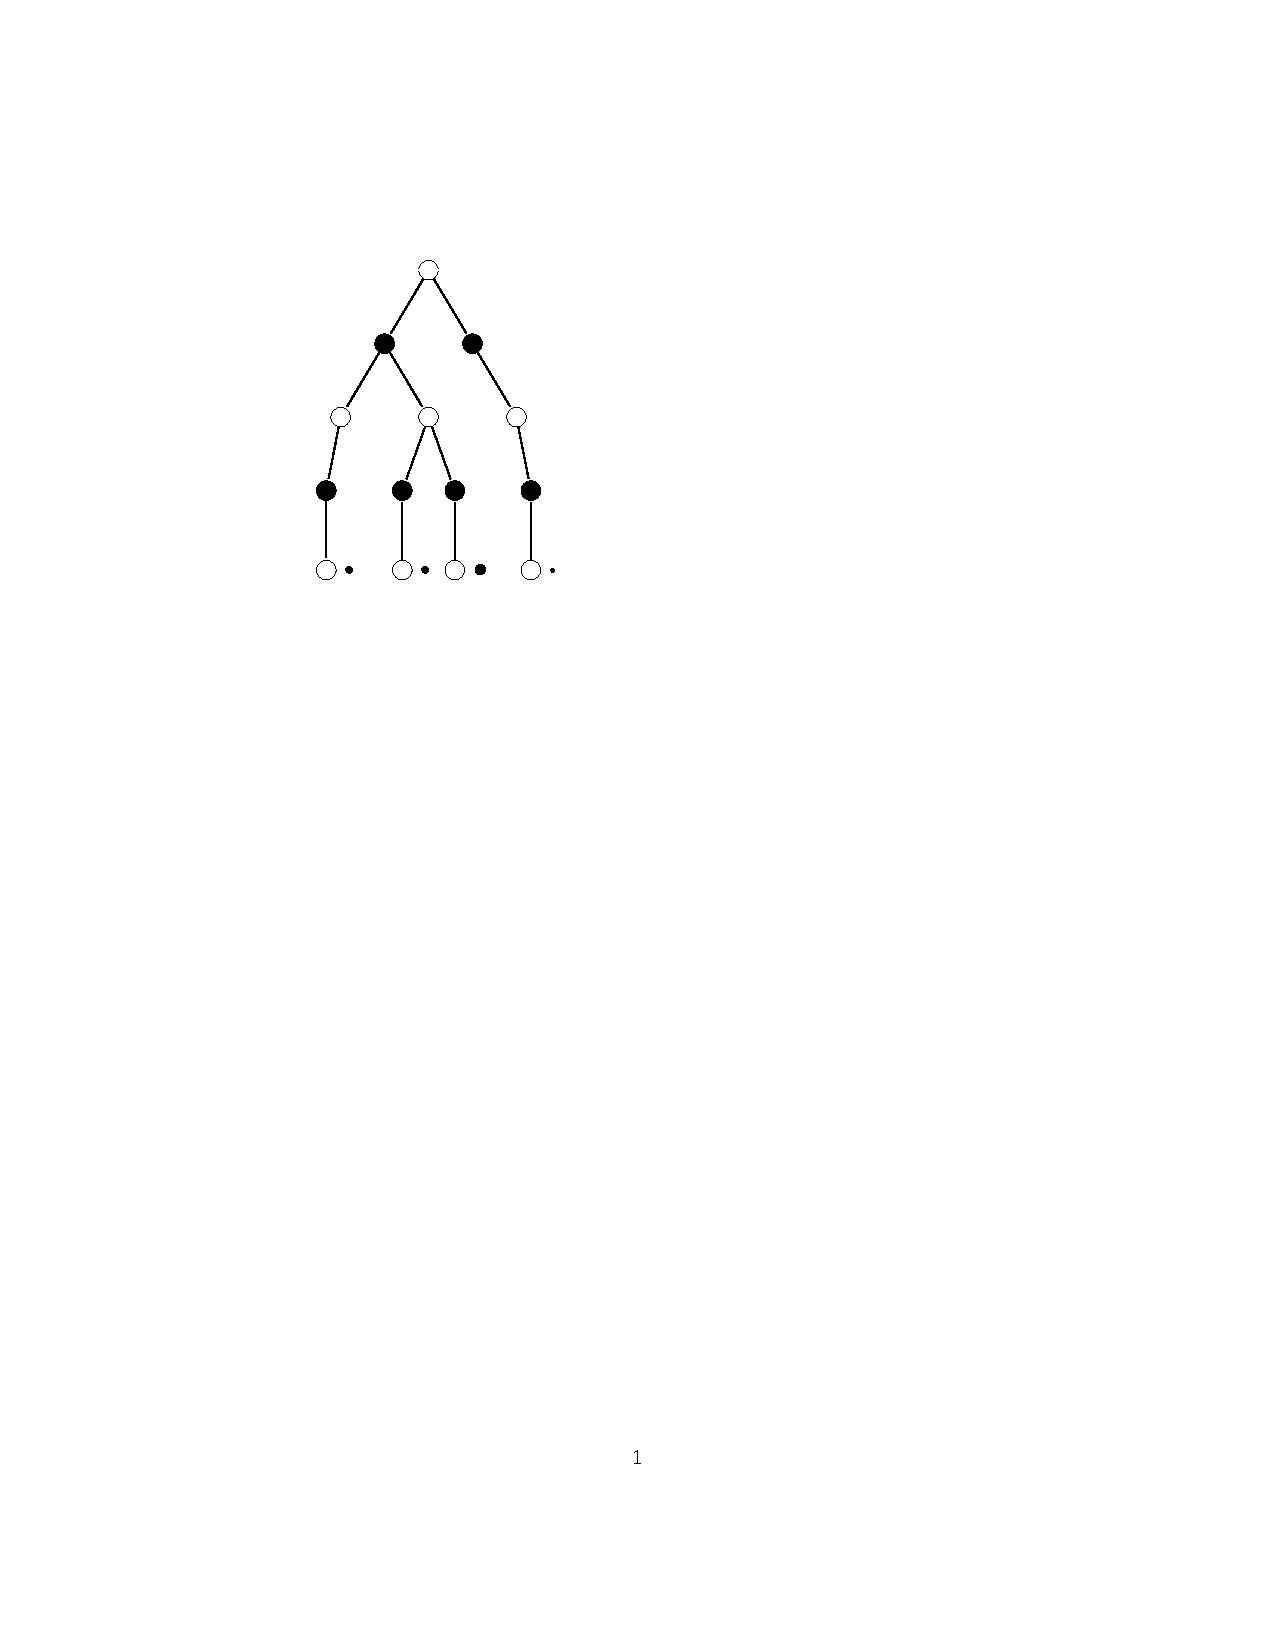
\includegraphics[width=0.7\linewidth, trim={5cm 17cm 12cm 4cm},clip]{articles/smcp/figures/main_ts4.pdf}
  \caption{\textbf{Update:} New actions and states are sampled from the proposal distribution and model. The particle sizes are proportional to their importance weight $w_t$.  \vspace{3.5em} } %
  \label{fig:sub2}
\end{subfigure}\hspace{.03\linewidth}
\begin{subfigure}{.30\textwidth}
  \centering
  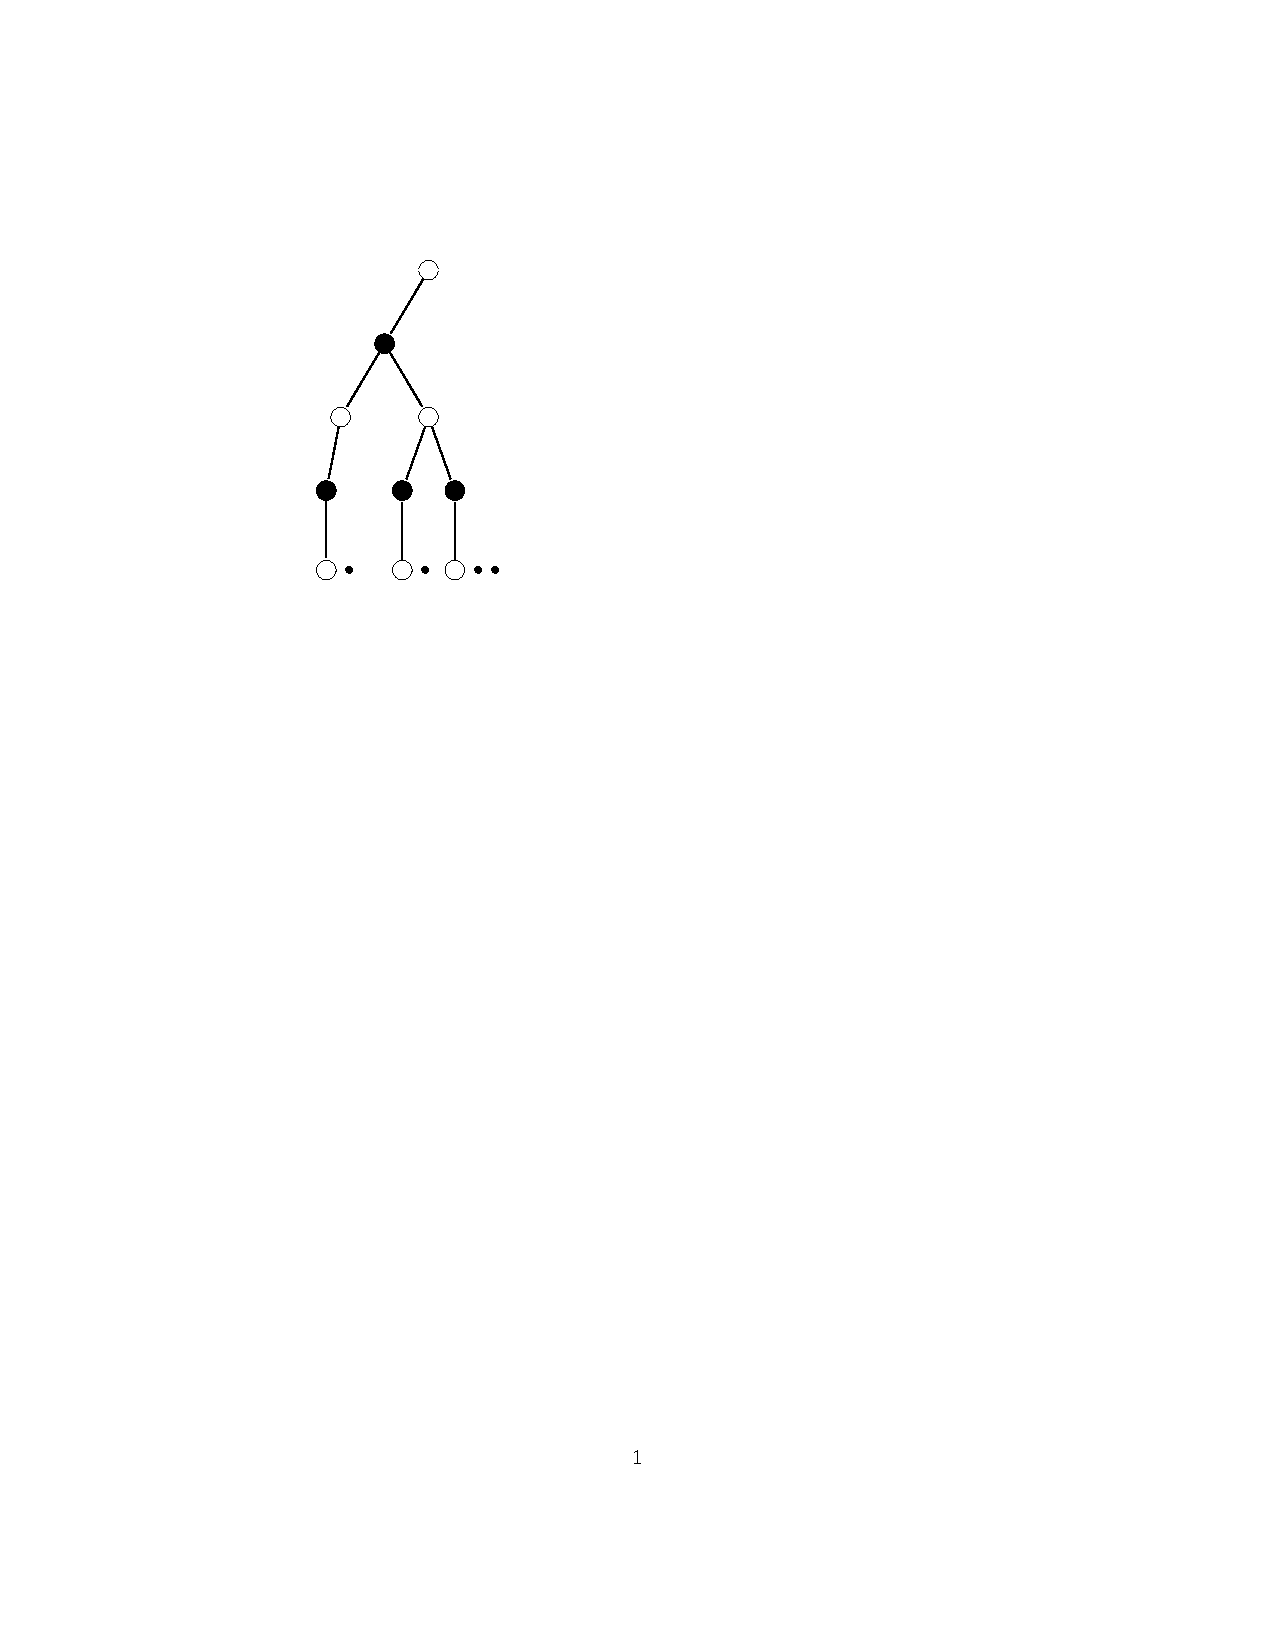
\includegraphics[width=0.7\linewidth, trim={5cm 17cm 12cm 4cm},clip]{articles/smcp/figures/main_ts5.pdf}
  \caption{\textbf{Resampling:} after sampling with replacement the particles relatively to their weight, the less promising branch was cut while the most promising has now two particles.\vspace{3em}}
  \label{fig:sub3}
\end{subfigure}
\caption{Schematic view of Sequential Monte Carlo planning. In each tree, the white nodes represent states and black nodes represent actions. Each bullet point near a state represents a particle, meaning that this particle contains the total trajectory of the branch. The root of the tree represents the root planning state, we expand the tree downward when planning.}
\label{fig:tree}
\end{figure}

\subsection{Optimism Bias and Control as Inference}
We now discuss shortcomings our approach to planning as inference may suffer from, namely encouraging risk seeking policies.

\paragraph*{Bias in the objective:} Trajectories having a high likelihood under the posterior defined in Equation~\ref{eq:posterior_target} are not necessarily trajectories yielding a high \textit{mean} return. Indeed, as 
$\log \E_p  \big[\exp R(\traj) \big] \ge  \E_p  \big[ R(\traj) \big]$
we can see that the objective function we maximize is an \textit{upper bound} on the quantity of interest: the mean return.
This can lead to risk-seeking trajectories as one very good outcome in $\log \E \exp$ could dominate all the other potentially very low outcomes, even if they might happen more frequently. This fact is alleviated when the dynamics of the environment are close to deterministic~\citep{levine2018reinforcement}. Thus, this bias does not appear to be very detrimental to us in our experiments~\ref{sec:exp} as our environments are fairly close to deterministic. The bias in the objective also appears in many control as inference works such as Particle Value Functions~\citep{maddison2017particle} and the probabilistic version of LQR proposed in~\cite{toussaint2009robot}.

\paragraph*{Bias in the model:} A distinct but closely related problem arises when one trains jointly the policy $\pi_\parampol$ and the model $\pmodel$, i.e if $q(\traj_{1:T})$ is directly trained to approximate $p(\traj_{1:T} | \gO_{1:T})$. In that case, $\pmodel(s_{t+1} | s_t, a_t)$ will not approximate $\penv(s_{t+1} | s_t, a_t)$ but $\penv(s_{t+1} | s_t, a_t, \gO_{t:T})$~\citep{levine2018reinforcement}. This means the model we learn has an optimism bias and learns transitions that are overly optimistic and do no match the environment's behavior.
This issue is simply solved by training the model separately from the policy, on transition data contained in a buffer as seen on line 18 of Algorithm~\ref{alg:sir_planning}.


\section{Experiments}
\subsection{Toy example}

In this section, we show how SMCP can deal with multimodal policies when planning.
We believe multimodality is useful for exploring since it allows us to keep a distribution over many promising trajectories and also allows us to adapt to changes in the environment e.g. if a path is suddenly blocked.

We applied two version of SMCP: i) with a resampling step (SIR) ii) without a resampling step (SIS) and compare it to CEM on a simple 2D point mass environment~\ref{fig:toy}. Here, the agent can control the displacement on $(x,y)$ within the square $[0,1]^2$, $a = (\Delta x, \Delta y)$ with maximum magnitude $||a|| = 0.05$. The starting position ($\bullet$) of the agent is $(x=0, y=0.5)$, while the goal ({\color{red} $\star$}) is at $g = (x=1, y=0.5)$. The reward is the agent's relative closeness increment to the goal: $r_t = 1- \frac{||s_{t+1} -g||^2}{||s_t -g||^2}$. However, there is a partial wall at the centre of the square leading to two optimal trajectories, one choosing the path below the wall and one choosing the path above.

The proposal is an isotropic normal distribution for each planning algorithm, and since the environment's dynamics are known, there is no need for learning: the only difference between the three methods is how they handle planning. We also set the value function to $0$ for SIR and SIS as we do not wish to perform any learning. We used $1500$ particles for each method, and updated the parameters of CEM until convergence. Our experiment~\ref{fig:toy} shows how having particles can deal with multimodality and how the resampling step can help to focus on the most promising trajectories. 



\begin{figure}
\begin{subfigure}{.295\textwidth}
\centering
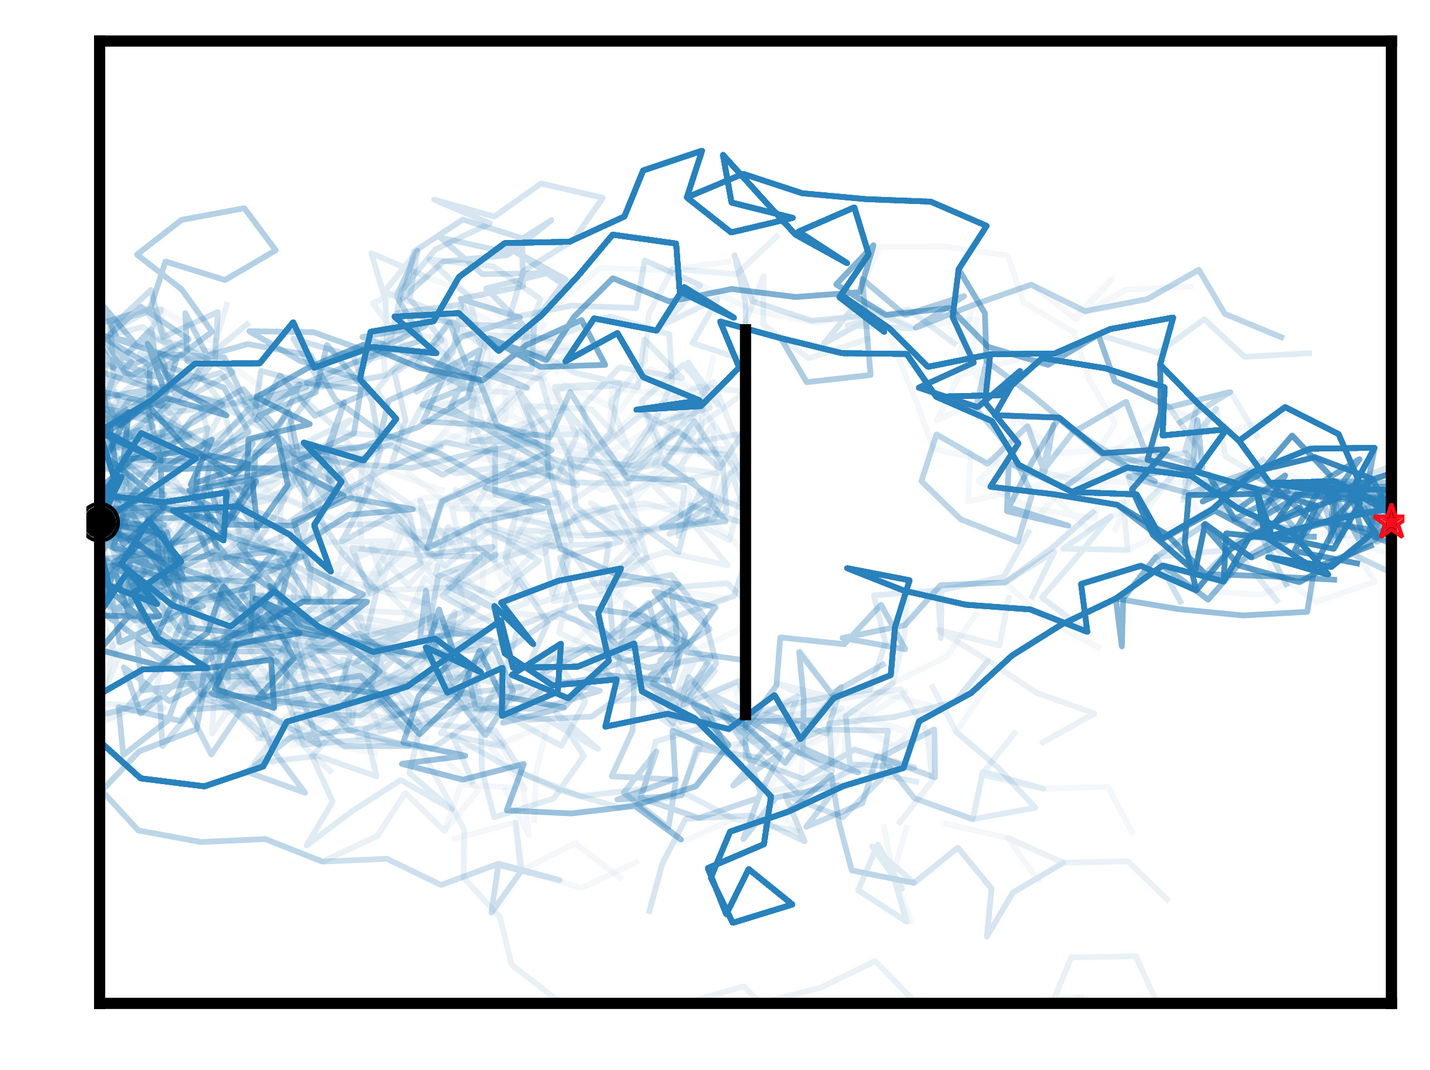
\includegraphics[width=\linewidth, trim={1.1cm 0cm .5cm 0cm},clip]{articles/smcp/figures/smc_resampling_true.png}
\caption{Sequential Importance Resampling (SIR): when resampling the trajectories at each time step, the agent is able to focus on the promising trajectories and does not collapse on a single mode.}
\label{fig:toy_sir}
\end{subfigure}\hspace{0.05\linewidth}
\begin{subfigure}{.295\textwidth}
\centering
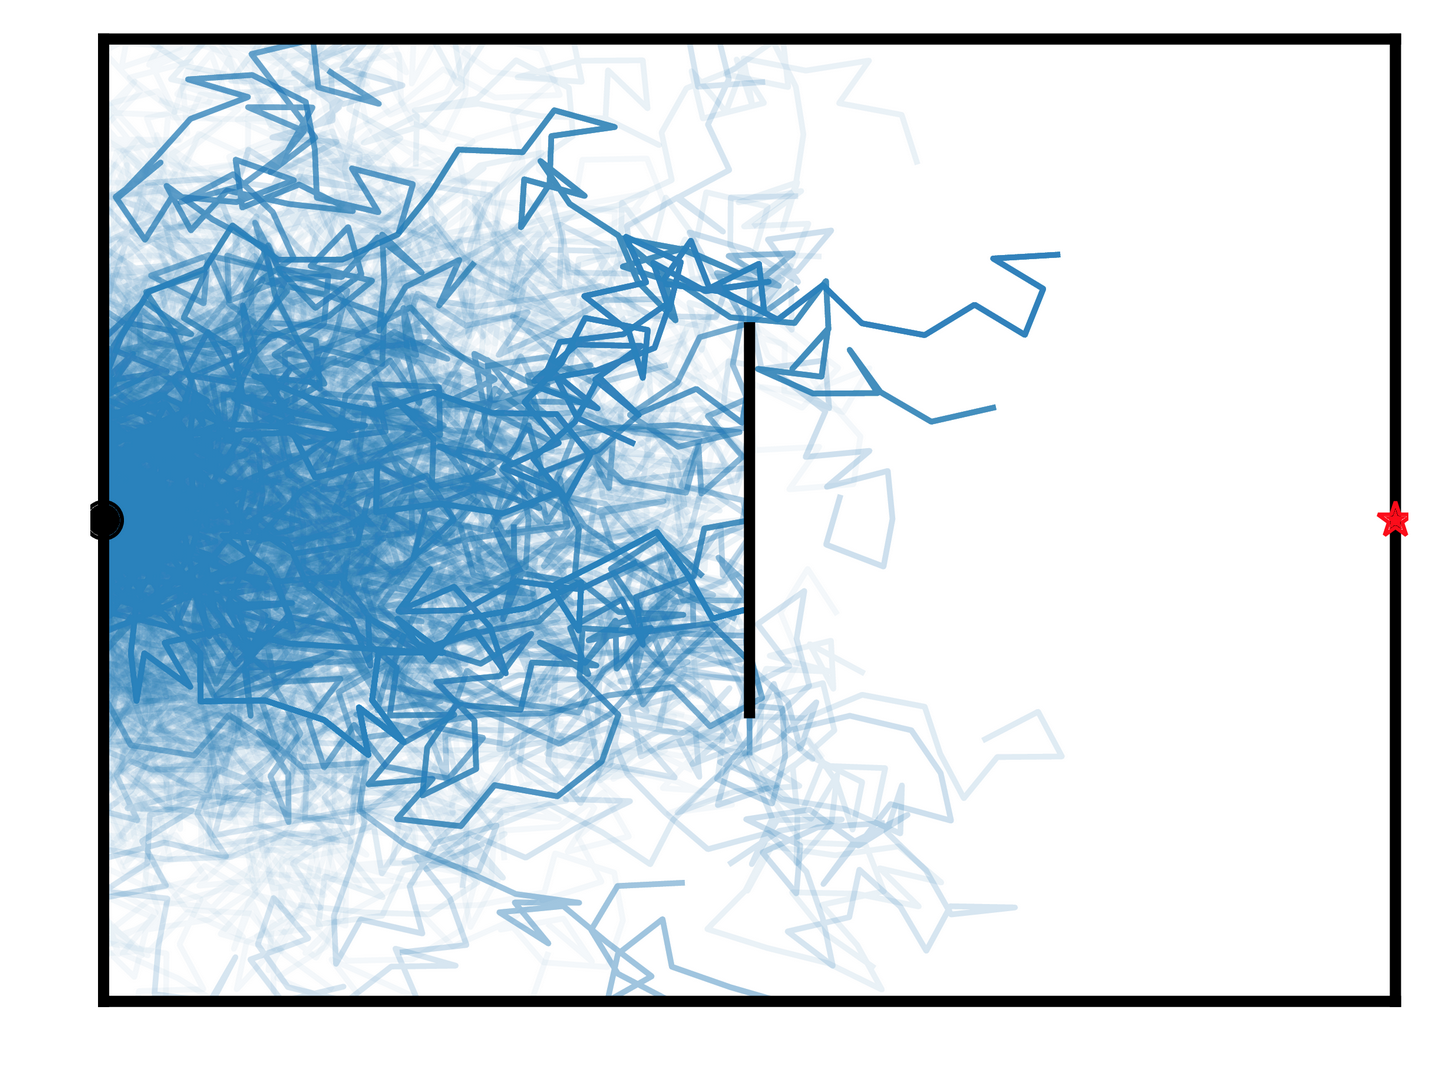
\includegraphics[width=\linewidth, trim={1.1cm 0cm .5cm 0cm},clip]{articles/smcp/figures/smc_resampling_false.png}
\caption{Sequential Importance Sampling (SIS): if we do not perform the resampling step the agent spends most of its computation on uninteresting trajectories and was not able to explore as well.\vspace{1em}}
\label{fig:toy_sis}
\end{subfigure}\hspace{0.05\linewidth}
\begin{subfigure}{.295\textwidth}
\centering
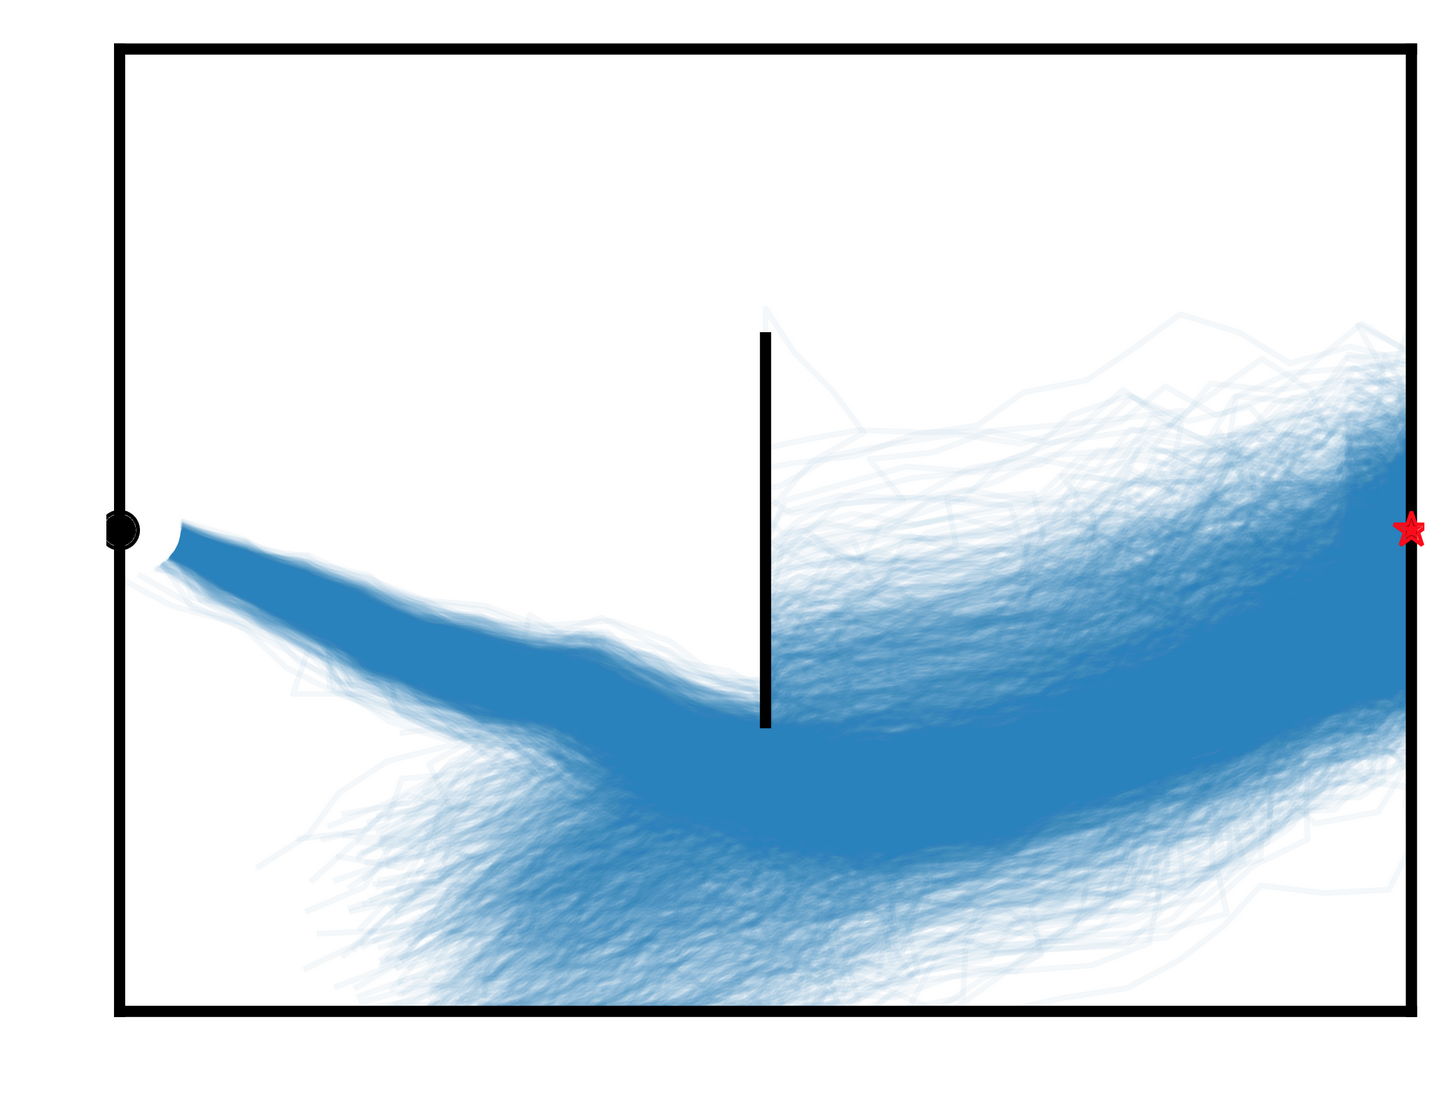
\includegraphics[width=\linewidth, trim={1.1cm 0cm .5cm 0cm},clip]{articles/smcp/figures/cem.png}
\caption{CEM: here the agent samples all the actions at once from a Gaussian with learned mean and covariance. We needed to update the parameters 50 times for the agent to find one solution, but it forgot the other one. }
\label{fig:toy_cem}
\end{subfigure}
\caption{Comparison of three methods on the toy environment. The agent ($\bullet$) must go to the goal ({\color{red}$\star$}) while avoiding the wall (\ \textbf{\textbar}\ ) in the center. The proposal distribution is taken to be an isotropic gaussian.  Here we plot the planning distribution imagined at $t=0$ for three different agents.  A darker shade of blue indicates a higher likelihood of the trajectory. Only the agent using Sequential Importance Resampling was able to find good trajectories while not collapsing on a single mode.}
\label{fig:toy}
\end{figure}

\subsection{Continuous Control Benchmark}
\label{sec:exp}

The experiments were conducted on the Open AI Gym Mujoco benchmark suite \citep{brockman2016openai, todorov2012mujoco}. To understand how planning can increase the learning speed of RL agents we focus on the 250000 first time steps. The Mujoco environments provide a complex benchmark with continuous states and actions that requires exploration in order to achieve state-of-the-art performances. 

The environment model used for our planning algorithm is the same as the probabilistic neural network used by \citet{chua2018deep}, it minimizes a gaussian negative log-likelihood model: 
\begin{equation*}
    \mathcal{L}_{\text{Gauss}}(\theta)= \tfrac{1}{2}\sum_{n=1}^N[\mu_\theta(s_n, a_n)-(s_{n+1}-s_n)]^\top\Sigma^{-1}_\theta(s_n, a_n)[\mu_\theta(s_n, a_n)-(s_{n+1}-s_n)]+\log \text{det} \Sigma_\theta(s_n, a_n),
\end{equation*}

where $\Sigma_\theta$ is diagonal and the transitions $(s_n, a_n, s_{n+1})$ are obtained from the environment.%





We included two popular planning algorithms on Mujoco as baselines: CEM \citep{chua2018deep} and Random Shooting (RS) \citep{nagabandi2017neural}. Furthermore, we included SAC \citep{haarnoja2018soft}, a model free RL algorithm, since i) it has currently one of the highest performances on Mujoco tasks, which make it a very strong baseline, and ii) it is a component of our algorithm, as we use it as a proposal distribution in the planning phase.

Our results suggest that SMCP does not learn as fast as CEM and RS initially as it heavily relies on estimating a good value function. However, SMCP quickly achieves higher performances than CEM and RS. SMCP also learns faster than SAC because it was able to leverage information from the model early in training. We hypothesize that the lack of performance gain of SMCP over SAC in the Hopper environment is due to the low quality of its model and the complexity of the task.

Note that our results differ slightly from the results usually found in the model-based RL literature. This is because we are tackling a more difficult problem: estimating the transitions and the reward function. We are using unmodified versions of the environments which introduces many hurdles. For instance, the reward function is challenging to learn from the state and very noisy. %

As in~\citet{henderson2017deep}, we assess the significance of our results by running each algorithm with multiple seeds ($10$ random seeds in our case, from seed $0$ to seed $9$). %






\begin{figure}
\centering
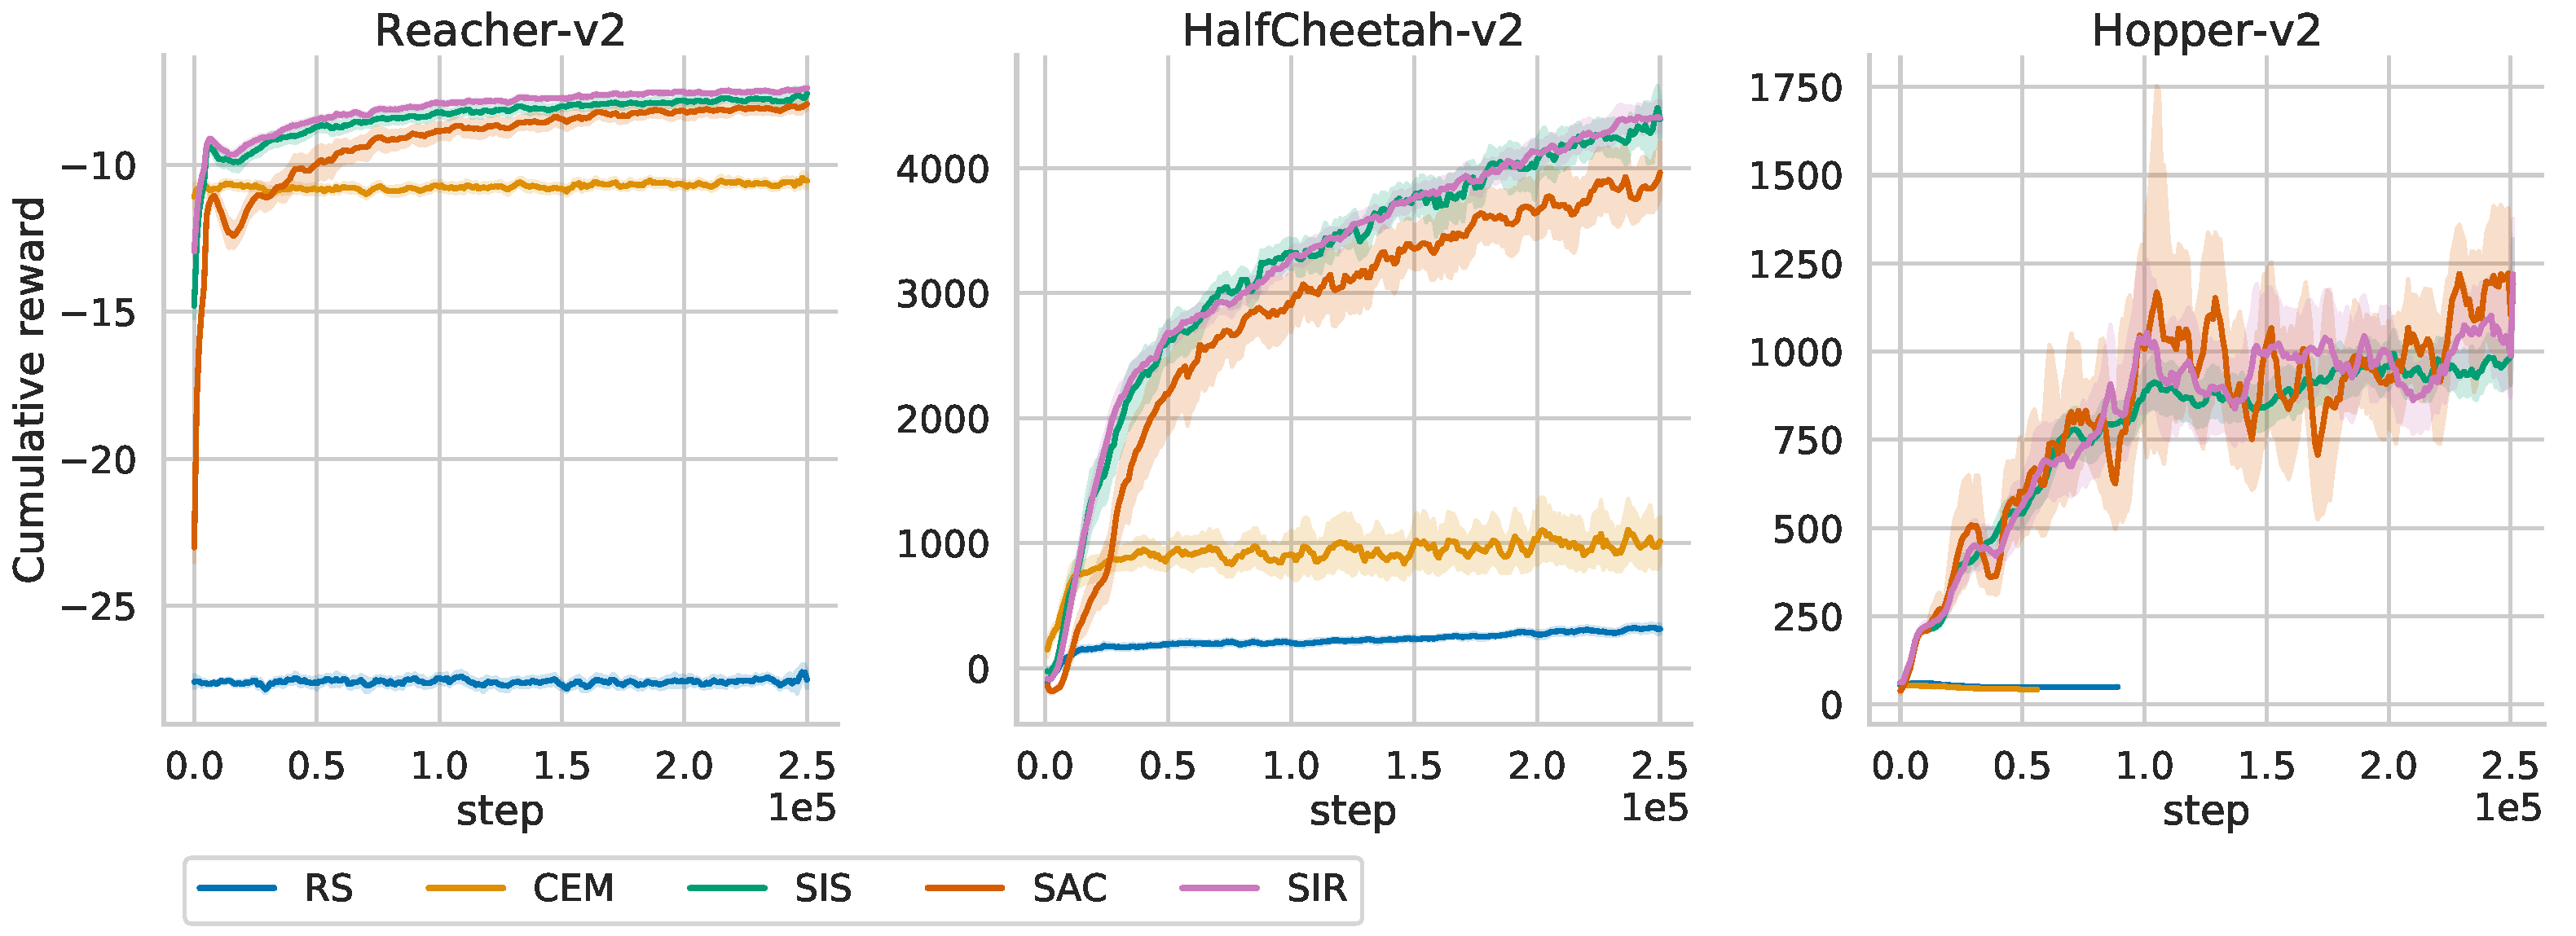
\includegraphics[width=\linewidth]{articles/smcp/figures/finalplotsmcp.pdf}
\caption{
Training curves on the Mujoco continuous control benchmarks. Sequential Monte Carlo Planning both with resampling (SIR) (pink) and without (SIS) (orange) learns faster than the Soft Actor-Critic model-free baseline (blue) and achieves higher asymptotic performances than the planning methods (Cross Entropy Methods and Random Shooting). The shaded area represents the standard deviation estimated by bootstrap over 10 seeds as implemented by the Seaborn package.  %
}
\label{fig:reward_new}
\end{figure}









\section{Conclusion and Future Work}
In this work, we have introduced a connection between planning and inference and showed how we can exploit advances in deep learning and probabilistic inference to design a new efficient and theoretically grounded planning algorithm. 
We additionally proposed a natural way to combine model-free and model-based reinforcement learning for planning based on the SMC perspective.
We empirically demonstrated that our method achieves state of the art results on Mujoco. Our result suggest that planning can lead to faster learning in control tasks.

However, our particle-based inference method suffers some several shortcomings. First, we need many particles to build a good approximation of the posterior, and this can be computationally expensive since it requires to perform a forward pass of the policy, the value function and the model for every particle. Second, resampling can also have adverse effects, for instance all the particles could be resampled on the most likely particle, leading to a particle degeneracy. More advanced SMC methods dealing with this issue such as backward simulation~\citep{lindsten2013backward} or Particle Gibbs with Ancestor Sampling (PGAS)~\citep{lindsten2014particle} have been proposed and using them would certainly improve our results.

Another issue we did not tackle in our work is the use of models of the environment learned from data. Imperfect model are known to result in compounding errors for prediction over long sequences. We chose to re-plan at each time step (Model Predictive Control) as it is often done in control to be more robust to model errors. More powerful models or uncertainty modeling techniques can also be used to improve the accuracy of our planning algorithm.
While the inference and modeling techniques used here could be improved in multiple ways, SMCP achieved impressive learning speed on complex control tasks. The planning as inference framework proposed in this work is general and could serve as a stepping stone for further work combining probabilistic inference and deep reinforcement learning.

























\chapter{On the Interplay between Noise and Curvature\\ and its Effect on Optimization and Generalization}
\label{chapter:hfc}





\section*{Article details}
Thomas V, Pedregosa F, Merriënboer B, Manzagol PA, Bengio Y, Le Roux N. ``On the interplay between noise and curvature and its effect on optimization and generalization''. In \emph{International Conference on Artificial Intelligence and Statistics (AISTATS) 2020. PMLR.}

\section*{Foreword}
This project started while I was thinking about the role of the stochasticity in SGD and its influence on generalization. At the same time, Nicolas Le Roux gave a talk at Mila where he mentioned a link between generalization, curvature and gradient noise in supervised learning. This started a collaboration which ultimately led to this paper published at AISTATS 2020. 

\section*{Impact since publication}
This work has inspired others such as~\citet{naganuma2022takeuchis} which validated our results by performing experiments at a larger scale than we did, \citet{rame2022fishr} used our empirical results on the similarity between the empirical and the true Fisher matrix and \citet{schneider2021cockpit} implemented the Takeuchi Information Criterion and approximations we developed for it as part of their package.



\section*{Personal contribution}
\begin{itemize}
    \item Making the link between our original idea and the already existing paper \citet{takeuchi1976distribution} which introduced the estimator first, was only published in Japanese and even reinvented later~\citep{murata1994network}.
    \item Performing all the large-scale experiments: training hundreds of neural networks with different parameters and architectures and datasets and recording useful statistics
    \item Theory and experiments for the link between the Hessian $\rmH$, the Fisher matrix $\rmF$ and the uncentered gradient covariance matrix $\rmC$
    \item Optimization theory for SGD and the interplay between $\rmH$ and $\rmC$ in the quadratic case
    \item Writing of the paper with Nicolas and created the figures
\end{itemize}

\begin{abstract}
    The speed at which one can minimize an expected loss using stochastic methods depends on two properties: the curvature of the loss and the variance of the gradients. While most previous works focus on one or the other of these properties, we explore how their interaction affects optimization speed. Further, as the ultimate goal is good generalization performance, we clarify how both curvature and noise are relevant to properly estimate the generalization gap. Realizing that the limitations of some existing works stems from a confusion between these matrices, we also clarify the distinction between the Fisher matrix, the Hessian, and the covariance matrix of the gradients.
\end{abstract}

\setcounter{footnote}{0}

\section{Introduction}


Training a machine learning model is often cast as the minimization of a smooth function $f$ over parameters $\theta$ in $\mathbb{R}^d$. More precisely, we aim at finding a minimum of an expected loss, i.e.
\begin{align}
    \theta^\ast &\in \arg\min_\theta \E_{p} [\mathcal{L}(\theta, x)] \; ,
\end{align}
where the expectation is under the data distribution $x \sim p$. In practice, we only have access to an empirical distribution $\hat{p}$ over $x$ and minimize the training loss
\begin{align}
    \hat{\theta}^\ast   &\in \arg\min_\theta \E_{\hat{p}}[\mathcal{L}(\theta, x)]\\
                        &= \arg\min_\theta f(\theta) \; .
\end{align}
To minimize this function, we assume access to an oracle which, for every value of $\theta$ and $x$, returns both $\mathcal{L}(\theta, x)$ and its derivative with respect to $\theta$, i.e., $\nabla_\theta \mathcal{L}(\theta, x)$. Given this oracle, stochastic gradient iteratively performs the following update: $\theta_{t+1} = \theta_t - \alpha_t \nabla \mathcal{L}(\theta_t, x)$~\footnote{We omit the subscripts when clear from context.} where $\{\alpha_t\}_{t \geq 0}$ is a sequence of stepsizes.

Two questions arise: First, how quickly do we converge to $\hat{\theta}^\ast$ and how is this speed affected by properties of $\mathcal{L}$ and $\hat{p}$? Second, what is $\E_{p}[\mathcal{L}(\hat{\theta}^\ast, x)]$?

It is known that the former is influenced by two quantities: the curvature of the function, either measured through its smoothness constant or its condition number, and the noise on the gradients, usually measured through a bound on $\E_{\hat{p}}[\|\nabla \mathcal{L}(\theta, x)\|^2]$. For instance,  when $f$ is $\mu$-strongly convex, $L$-smooth, and the noise is bounded, i.e. $\E_{\hat{p}}[\|\nabla\mathcal{L}(\theta, x)\|^2] \leq c$, then stochastic gradient with a constant stepsize $\alpha$ will converge linearly to a ball~\citep{schmidt2014convergence}. Calling $\Delta$ the suboptimality, i.e. $\Delta_k = f(\theta_k) - f(\hat{\theta}^\ast)$, we have
\begin{align}
    \label{eq:sg_cvg_rate}
    \E [\Delta_k]   &\leq (1 - 2\alpha\mu)^k \Delta_0 + \frac{L\alpha c}{4\mu} \; .
\end{align}

This implies that as $k\to \infty$, the expected suboptimality depends on both the curvature through $\mu$ and $L$, and on the noise through $c$. However, bounding curvature and noise using constants rather than full matrices hides the dependencies between these two quantities. We also observed that, because existing works replace the full noise matrix with a constant when deriving convergence rates, that matrix is poorly understood and is often confused with a curvature matrix.
This confusion remains when discussing the generalization properties of a model. Indeed, the generalization gap stems from a discrepancy between the empirical and the true data distribution. An estimator of this gap must thus include an estimate of that discrepancy in addition to an estimate of the impact of an infinitesimal discrepancy on the loss. The former can be characterized as noise and the latter as curvature. Hence, attempts at estimating the generalization gap using only the curvature~\citep{keskar2016large,novak2018sensitivity} are bound to fail as do not characterize the size or geometry of the discrepancy.

In this work, we make the following contributions:
\begin{itemize}
    \item We provide theoretical and empirical evidence of the similarities and differences surrounding the curvatures matrices; the Fisher $\rmF$ and the Hessian $\rmH$, and the noise matrix, $\rmC$;
    \item We briefly expand the convergence results of~\citet{schmidt2014convergence}, theoretically and empirically highlighting the importance of the relationship between noise and curvature for strongly convex functions and quadratics;
    \item We make the connection with an old estimator of the generalization gap, the Takeuchi Information Criterion, and show how its use of both curvature and noise yields a superior estimator to other commonly used ones, such as flatness or sensitivity for neural networks.
\end{itemize}

\section{Information matrices: definitions, similarities, and differences}
\label{sec:hfc}
Before delving into the impact of the information matrices for optimization and generalization, we start by recalling their definitions. We shall see that, despite having similar formulations, they encode different information. We then provide insights on their similarities and differences.

We discuss here two information matrices associated with curvature, the Fisher matrix $\rmF$ and the Hessian $\rmH$, and one associated with noise, the gradients' uncentered covariance $\rmC$. In particular, while $\rmF$ and $\rmH$ are well understood, $\rmC$ is often misinterpreted. For instance, it is often called ``empirical Fisher''~\citep{martens2014new} despite bearing no relationship to $\rmF$, the true Fisher. This confusion can have dire consequences and optimizers using $\rmC$ as approximation to $\rmF$ can have arbitrarily poor performance~\citep{kunstner2019limitations}.

To present these matrices, we consider the case of maximum likelihood estimation (MLE). We have access to a set of samples $(x,y) \in \gX \times \gY$ where $x$ is the input and $y$ the target. We define $p: \gX \times \gY \mapsto \sR$ as the \textbf{data distribution} and $\q: \gX \times \gY \mapsto \sR$ such that $\q(x,y) = p(x) \q(y|x)$ as the \textbf{model distribution}\footnote{$\q(y|x)$ are the softmax activations of a neural network in the classification setting.}.
For each sample $(x, y) \sim p$, our loss is the negative log-likelihood $\mathcal{L}(\theta, y,x) = - \log \q(y|x)$.
Note that all the definitions and results in this section are valid whether we use the true data distribution $p$ or the empirical $\hat{p}$.

Matrices $\rmH$, $\rmF$ and $\rmC$ are then defined as:

\begin{align}
\rmH(\theta) &= \E_{\color{darkorchid}{p}}\color{cerulean}{\left[\frac{\partial^2 }{\partial \theta \partial \theta^\top} \mathcal{L}(\theta, y,x)\right]} \label{eq:def_h}\\
\rmC(\theta) &= \E_{\color{darkorchid}{p}}\color{burntorange}{\left[\frac{\partial}{\partial \theta }\mathcal{L}(\theta, y,x) \frac{\partial}{\partial \theta }\mathcal{L}(\theta, y,x)^\top\right]} \label{eq:def_c}\\
\rmF(\theta) &= \E_{\color{dartmouthgreen}{q_\theta}}\color{burntorange}{\left[\frac{\partial}{\partial \theta }\mathcal{L}(\theta, y,x) \frac{\partial}{\partial \theta }\mathcal{L}(\theta, y,x)^\top\right]} \label{eq:def_f1}\\
&= \E_{\color{dartmouthgreen}{q_\theta}}\color{cerulean}{\left[\frac{\partial^2 }{\partial \theta \partial \theta^\top} \mathcal{L}(\theta, y,x)\right]}  \; .\label{eq:def_f2}
\end{align}

We observe the following: a) The definition of $\rmH$ and $\rmC$ involves the data distribution, in contrast with the definition of $\rmF$, which involves the model distribution; b) If $\q = p$, all matrices are equal. Furthermore, as noted by~\citet{martens2014new}, $\rmH = \rmF$ whenever the matrix of second derivatives does not depend on $y$, a property shared in particular by all generalized linear models.

As said above, $\rmH$, $\rmF$, and $\rmC$ characterize different properties of the optimization problem. $\rmH$ and $\rmF$ are curvature matrices and describe the geometry of the space around the current point. $\rmC$, on the other hand, is a ``noise matrix'' and represents the sensitivity of the gradient to the particular sample.\footnote{Technically, it is $\rmS$, the centered covariance matrix, rather than $\rmC$ which plays that role but the two are similar close to a stationary point.}

We now explore in more details their similarities and differences.

\subsection{Bounds between \texorpdfstring{$\rmH$}{H}, \texorpdfstring{$\rmF$}{F} and \texorpdfstring{$\rmC$}{C}}
The following proposition bounds the distance between the information matrices:


\begin{proposition}[Distance between $\rmH, \rmF$ and $\rmC$]
Assuming the second moments of the Fisher are bounded above, i.e. $ \E_{\q} [ ||\nabla_\theta^2 \mathcal{L}(\theta, x, y)||^2] \leq \beta_1$ and \\ $\E_{\q} [ ||\nabla_\theta \mathcal{L}(\theta, x, y) \nabla_\theta \mathcal{L}(\theta, x, y)^\top||^2] \leq \beta_2$, we have
\begin{eqnarray*}
||\rmF - \rmH||^2 &\le& \beta_1 \ \gD_{\chi^2}(p||\q) \; ,\\
||\rmF - \rmC||^2 &\le&  \beta_2 \ \gD_{\chi^2}(p||\q) \; ,\\
||\rmC - \rmH||^2 &\le&  \big(\beta_1 + \beta_2\big) \ \gD_{\chi^2}(p||\q) \; .
\end{eqnarray*}
where $\gD_{\chi^2}(p||\q) = \iint \tfrac{(p(x, y)-\q(x, y))^2}{\q(x, y)} dy dx $ is the $\chi^2$ divergence and $|| \cdot ||$ is the Frobenius norm.
\end{proposition}
All the proofs are in the appendix.

In particular, when $p = \q$ we recover that $\rmF = \rmH = \rmC$. At first glance, one could assume that, as the model is trained and $q_\theta$ approaches $p$, these matrices become more similar. The $\chi^2$ divergence is however poorly correlated with the loss of the model. One sample where the prediction of the model is much smaller than the true distribution can dramatically impact the $\chi^2$ divergence and thus the distance between the information matrices. We show in Section~\ref{sec:HFC_diff} how these distances evolve when training a deep network.

\subsection{\texorpdfstring{$\rmC$}{C} does not approximate \texorpdfstring{$\rmF$}{F}}
\label{sec:C_is_not_F}
$\rmC$ is often referred to as the ``empirical Fisher'' matrix, implying that it is an approximation to the true Fisher matrix $\rmF$~\citep{martens2014new}. In some recent works~\citep{liang2017fisher, george2018fast} the empirical Fisher matrix is used instead of the Fisher matrix.
However, in the general case, there is no guarantee that $\rmC$ will approximate $\rmF$, even in the limit of infinite samples. We now give a simple example highlighting their different roles:
\begin{example}[Mean regression]
Let $X = (x_i)_{i=1, \dots, N}$ be an i.i.d sequence of random variables. The task is to estimate $\mu = \E [x]$ by minimizing the loss $ \mathcal{L}(\theta) = \frac{1}{2 N} \sum_{n=1}^N||x_n - \theta||^2 $. The minimum is attained at $\thetamle= \frac{1}{N} \sum_{n=1}^N x_n$. This estimator is consistent and converges to $\mu$ at rate $\mathcal{O}(\tfrac{1}{\sqrt{N}})$.

This problem is an MLE problem if we define $\q(x) = \mathcal{N}(x; \theta, \rmI_d)$. In this case, we have
\begin{align}
\label{eq:HFC}
\rmH(\thetamle) = \rmF(\thetamle) = \rmI_d\quad &, \quad \rmC(\thetamle) = \widehat{\rmSS}_x \; ,
\end{align}
where $\widehat{\rmSS}_x$ is the empirical covariance of the $x_i$'s. We see that, even in the limit of infinite data, the covariance $\rmC$ does not converge to the actual Fisher matrix nor the Hessian. Hence we shall and will not refer to $\rmC$ as the ``empirical Fisher'' matrix.
\end{example}

In some other settings, however, one can expect a stronger correlation between $\rmC$ and $\rmH$:
\begin{example}(Ordinary Least Squares)
Let us assume we have a data distribution $(x_n, y_n)$ so that
\begin{equation}\label{eq:linear_model}
    y_n = x_n^\top \theta^\ast  + \epsilon_n, \quad \epsilon_n \sim \mathcal{N}(0, \rmSS)
\end{equation}
with $y_n \in \sR^p$ and $x_n, \epsilon_n \in \sR^d$, $\theta \in \sR^{p \times d}$.
We train a model to minimize the sum of squares residual
\begin{equation}
\min_\theta\frac{1}{2 N} \sum_{n=1}^N || y_n - x_n^\top\theta ||^2 \; .
\end{equation}
In that case, for $\theta = \theta^\ast$
\begin{align}
\label{eq:HFC_OLS}
\rmH = \rmF = \E_p [ x x^\top ] \quad &, \quad \rmC =\E_p [ x \rmSS x^\top ]  \; 
\end{align}
First, we observe that the Hessian and the Fisher are equal, for all $\theta$. Second, when the input/output covariance matrix is isotropic $\rmSS=\sigma^2 \rmI$, then we have $\rmC \propto \rmH = \rmF$. 
\end{example}

\section{Information matrices in optimization}
\label{sec:optimization}
Now that the distinction between these matrices has been clarified, we can explain how their interplay affects optimization. In this section, we offer theoretical results, as well as a small empirical study, on the impact of the noise geometry on convergence rates.

\subsection{Convergence rates}
We start here by expanding the the result of~\citet{schmidt2014convergence} to full matrices, expliciting how the interplay of noise and curvature affects optimization. We then build a toy experiment to validate the results.

\subsubsection{General setting}

\begin{proposition}[Function value]
\label{prop:function_value}
Let $f$ be a twice-differentiable function. Assume $f$ is $\mu$-strongly convex and there are two matrices $\rmH$ and $\rmS$ such that for all $\theta$, $\theta'$:
\begin{align*}
    f(\theta') &\leq f(\theta) + \nabla f(\theta)^\top(\theta' - \theta) + \frac{1}{2} (\theta' - \theta)^\top \rmH (\theta' - \theta)\\
    &\E_p[\nabla \mathcal{L} (\theta, x) \nabla \mathcal{L} (\theta, x)^\top] \preccurlyeq \rmS + \nabla f(\theta) \nabla f(\theta)^\top\; .
\end{align*}
Then stochastic gradient with stepsize $\alpha$ and positive definite preconditioning matrix $\rmM$ satisfies
\begin{align*}
    \E [\Delta_k]   &\leq (1 - 2\alpha\mu_M\mu)^k \Delta_0 + \frac{\alpha}{4\mu_{M} \mu }\Tr(\rmH \rmM \rmS \rmM) \; ,
\end{align*}
where $\mu_M$ is the smallest eigenvalue of\, $\rmM - \frac{\alpha}{2} \rmM^\top \rmH \rmM$.
\end{proposition}

$\rmS$ is the centered covariance matrix of the stochastic gradients and, if $f$ is quadratic, then $\rmH$ is the Hessian.




\subsubsection{Centered and uncentered covariance}
Proposition~\ref{prop:function_value}, as well as most results on optimization, uses a bound on the uncentered covariance of the gradients. The result is that the noise must be lower far away from the optimum, where the gradients are high. Thus, it seems more natural to define convergence rates as a function of the \emph{centered} gradients' covariance $\rmS$, although these results are usually weaker as a consequence of the relaxed assumption. For the remainder of this section, focused on the quadratic case, we will use $\rmS$. Note that the two matrices are equal at any first-order stationary point.

Centered covariance matrices have been used in the past to derive convergence rates, for instance by~\citet{bach2013non,flammarion2015averaging,dieuleveut2016nonparametric}. These works also include a dependence on the geometry of the noise since their constraint is of the form $\rmS \preccurlyeq \sigma^2 \rmH$. In particular, if $\rmS$ and $\rmH$ are not aligned, $\sigma^2$ must be larger for the inequality to hold.

\subsubsection{Quadratic functions}
\begin{proposition}[Quadratic case]
\label{prop:quadratic}
Assuming we minimize a quadratic function $$f(\theta) = \tfrac{1}{2} (\theta - \hat\theta^\ast)^\top \rmH (\theta-\hat\theta^\ast)$$ only having access to a noisy estimate of the gradient $g(\theta) \sim \nabla f(\theta) + \epsilon$ with $\epsilon$ a zero-mean random variable with covariance $\E [\epsilon \epsilon^\top ] = \rmS$, then the iterates obtained using stochastic gradient with stepsize $\alpha$ and preconditioning psd matrix $\rmM$ satisfy
\begin{align*}
    \E [\theta^k - \hat\theta^\ast] &= (1 - \alpha \rmM \rmH)^k (\theta^0 - \hat\theta^\ast) \; .
\end{align*}
Further, the covariance of the iterates $\rmSS_k = {\E [ (\theta^k-\hat\theta^\ast) (\theta^k-\hat\theta^\ast)^\top]} $ satisfies
\begin{align*}
    \rmSS_{k+1} &=  (\rmI  -\alpha \rmM \rmH) \rmSS_{k}  (\rmI  -\alpha \rmM \rmH)^\top + \alpha^2 \rmM \rmS \rmM^\top\; .
\end{align*}
In particular, the stationary distribution of the iterates has a covariance $\rmSS_\infty$ which verifies the equation
\begin{align*}
    \rmSS_\infty \rmH \rmM + \rmM \rmH \rmSS_\infty &=  \alpha \rmM \big( \rmS + \rmH \rmSS_\infty \rmH\big) \rmM\; .
\end{align*}
\end{proposition}
Recently, analyzing the stationary distribution of SGD by modelling its dynamics as a stochastic differential equation (SDE) has gained traction in the machine learning community~\citep{chaudhari2017stochastic, jastrzkebski2017three}. Worthy of note, \citet{mandt2017stochastic, zhu2018anisotropic} do not make assumptions about the structure of the noise matrix $\rmS$. Our proposition above extends and corrects some of their results as it does not rely on the continuous-time approximation of the dynamics of SGD. Indeed, as pointed out in~\citet{yaida2018fluctuation}, most of the works using the continuous-time approximation implicitly make the confusion between centered $\rmS$ and uncentered $\rmC$ covariance matrices of the gradients.

\begin{proposition}[Limit cycle of SG]
\label{prop:sg_limit} 
If $f$ is a quadratic function and $\rmH$, $\rmC$ and $\rmM$ are simultaneously diagonalizable, then stochastic gradient with symmetric positive definite preconditioner $\rmM$ and stepsize $\alpha$ yields
\begin{align}
\E[\Delta_t]  &= \tfrac{\alpha}{2} \Tr ((2 \rmI - \alpha \rmM \rmH)^{-1} \rmM \rmS) + \gO(e^{-t}) \; .
\end{align}
\end{proposition}

Rather than using a preconditioner, another popular method to reduce the impact of the curvature is Polyak momentum, defined as
\begin{align*}
    v_0 &=0 \quad , \quad v_t = \gamma v_{t-1} + \nabla_\theta \mathcal{L}(\theta_t, x_t)\\
    \theta_{t+1}    &= \theta_t - \alpha v_t \; .
\end{align*}

\begin{proposition}[Limit cycle of momentum]
\label{prop:polyak_limit}
If $f$ is a quadratic function and $\rmH$ and $\rmC$ are simultaneously diagonalizable, then Polyak momentum with parameter $\gamma$ and stepsize $\alpha$ yields
\begin{align}
    \E[\Delta_t]    &= \tfrac{\alpha}{2} \tfrac{(1 + \gamma)}{(1 - \gamma)} \Tr \left((2 (1 + \gamma) \rmI - \alpha \rmH)^{-1} \rmS \right) + \gO(e^{-t}) \; .
\end{align}
\end{proposition}

\section{Generalization}
So far, we focused on the impact of the interplay between curvature and noise in the optimization setting. However, optimization, i.e. reaching low loss on the training set, is generally not the ultimate goal as one would rather reach a low test loss. The difference between training and test loss is called the generalization gap and estimating it has been the focus of many authors~\citep{keskar2016large, neyshabur2017exploring, liang2017fisher, novak2018sensitivity, rangamani2019scale}.

We believe there is a fundamental misunderstanding in several of these works, stemming from the confusion between curvature and noise. Rather than proposing a new metric, we empirically show how the Takeuchi information criterion~\citep[TIC:][]{takeuchi1976distribution} addresses these misunderstandings. It makes use of both the Hessian of the loss with respect to the parameters, $\rmH$, and the uncentered covariance of the gradients, $\rmC$. While the former represents the curvature of the loss, i.e., the sensitivity of the gradient to a change in parameter space, the latter represents the sensitivity of the gradient to a change in inputs. As the generalization gap is a direct consequence of the discrepancy between training and test sets, the influence of $\rmC$ is natural. Thus, our result further reinforces the idea that the Hessian cannot by itself be used to estimate the generalization gap, an observation already made by~\citet{dinh2017sharp}, among others.

\subsection{Takeuchi information criterion}
In the simplest case of a well specified least squares regression problem, an unbiased estimator of the generalization gap is the AIC~\citep{akaike1974new}, which is simply the number of degrees of freedom divided by the number of samples: $\displaystyle\hat{\gG}(\theta) = \tfrac{1}{N} d$ where $d$ is the dimensionality of $\theta$. This estimator is valid locally around the maximum likelihood parameters computed on the training data.  However, these assumptions do not hold in most cases, leading to the number of parameters being a poor predictor of the generalization gap~\citep{novak2018sensitivity}.
When dealing with maximum likelihood estimation (MLE) in misspecified models, a more general formula for estimating the gap is given by the Takeuchi information criterion~\citep[TIC:][]{takeuchi1976distribution}:
\begin{align}
\label{eq:tic}
  \hat{\gG} &= \frac{1}{N} \Tr(\rmH(\hat\theta^\ast)^{-1} \rmC(\hat\theta^\ast))  \; ,
\end{align}
where $\hat\theta^\ast$ is a local optimum. Note that $\rmH$ and $\rmC$ here are the hessian and covariance of the gradients matrices computed on the \emph{true data distribution}.

This criterion is not new in the domain of machine learning. It was rediscovered by~\citet{murata1994network} and similar criteria have been proposed since then~\citep{beirami2017optimal, wang2018approximate}. However, as far as we know, no experimental validation of this criterion has been carried out for deep networks.
Indeed, for deep networks, $\rmH$ is highly degenerate, most of its eigenvalues being close to $0$~\citep{sagun2016eigenvalues}. In this work, the Takeuchi information criterion is computed, in the degenerate case, by only taking into account the eigenvalues of the Hessian of significant magnitude. In practice, we cut all the eigenvalues smaller than a constant times the biggest eigenvalue and perform the inversion on that subspace. Details can be found in appendix~\ref{app:inversion}.

Interestingly, the term $\Tr(\rmH^{-1}\rmC)$ appeared in several works before, whether as an upper bound on the suboptimality~\citep{flammarion2015averaging} or as a number of iterates required to reach a certain suboptimality~\citep{bottou2008tradeoffs}. Sadly, it is hard to estimate for large networks but we propose an efficient approximation in Section~\ref{sec:tic_approx}.



\subsection{Limitations of flatness and sensitivity}
We highlight here two commonly used estimators of the generalization gap as they provide good examples of failure modes that can occur when not taking the noise into account. This is not to mean that these estimators cannot be useful for the models that are common nowadays, rather that they are bound to fail in some cases.

\textbf{Flatness}~\citep{hochreiter1997flat} links the spectrum of the Hessian at a local optimum with the generalization gap. This correlation, observed again by~\citet{keskar2016large}, was already shown to not hold in general~\citep{dinh2017sharp}. As we showed in Section~\ref{sec:C_is_not_F}, the Hessian does not capture the covariance of the data, which is linked to the generalization gap through the central-limit theorem.

\textbf{Sensitivity}~\citep{novak2018sensitivity} links the generalization gap to the derivative of the loss with respect to the input. The underlying idea is that we can expect some discrepancy between train and test data, which will induce changes in the output and a potentially higher test loss. However, penalizing the norm of the Jacobian assumes that changes between train and test data will be isotropic. In practice, we can expect data to vary more along some directions, which is not reflected in the sensitivity. In the extreme case where the test data is exactly the same as the training data, the generalization gap will be 0, which will again not be captured by the sensitivity. In practice, whitening the data makes the sensitivity appropriate, save for a scaling factor, as we will see in the experiments.















\section{Experiments}
We now provide experimental validation of all the results in this paper. We start by analyzing the distance between information matrices, first showing its poor correlation with the training loss, then showing that these matrices appear to be remarkably aligned, albeit with different scales, when training deep networks on standard datasets.

\subsection{Discrepancies between \texorpdfstring{$\rmC$}{C}, \texorpdfstring{$\rmH$}{H} and \texorpdfstring{$\rmF$}{F}}
\label{sec:exp_hfc}

\subsubsection{Experimental setup}
\label{sec:exp_setup_hfc}
For comparing the similarities and discrepencies between the information matrices, we tested
\begin{itemize}
    \item 5 different architectures: logistic regression, a 1-hidden layer and 2-hidden layer fully connected network, and 2 small convolutional neural networks (CNNs, one with batch normalization~\citep{ioffe2015batch} and one without);
    \item 3 datasets: MNIST, CIFAR-10, SVHN;
    \item 3 learning rates: $10^{-2}$, $5\cdot 10^{-3}$, and $10^{-3}$, using SGD with momentum $\mu = 0.9$;
    \item 2 batch sizes: $64$, $512$;
    \item 5 dataset sizes: 5k, 10k, 20k, 25k, and 50k.
\end{itemize}
We train for 750k steps and compute the metrics every 75k steps. To be able to compute all the information matrices exactly, we reduced the input dimension by converting all images to greyscale and resizing them to $7 \times 7$ pixels. While this makes the classification task more challenging, our neural networks still exhibit the behaviour of larger ones by their ability to fit the training set, even with random labels. Details and additional figures can be found in appendix~\ref{app:exp_details}.

\subsection{Comparing Fisher and empirical Fisher}

Figure~\ref{fig:F_vs_C} shows the squared Frobenius norm between $\rmF$ and $\rmC$ (on training data) for many architectures, datasets, at various stages of the optimization. We see that, while the two matrices eventually coincide on the training set for some models, the convergence is very weak as even low training errors can lead to a large discrepancy between these two matrices. In practice, $\rmC$ and $\rmF$ might be significantly different, even when computed on the training set.

\begin{figure}[ht]
  \centering
    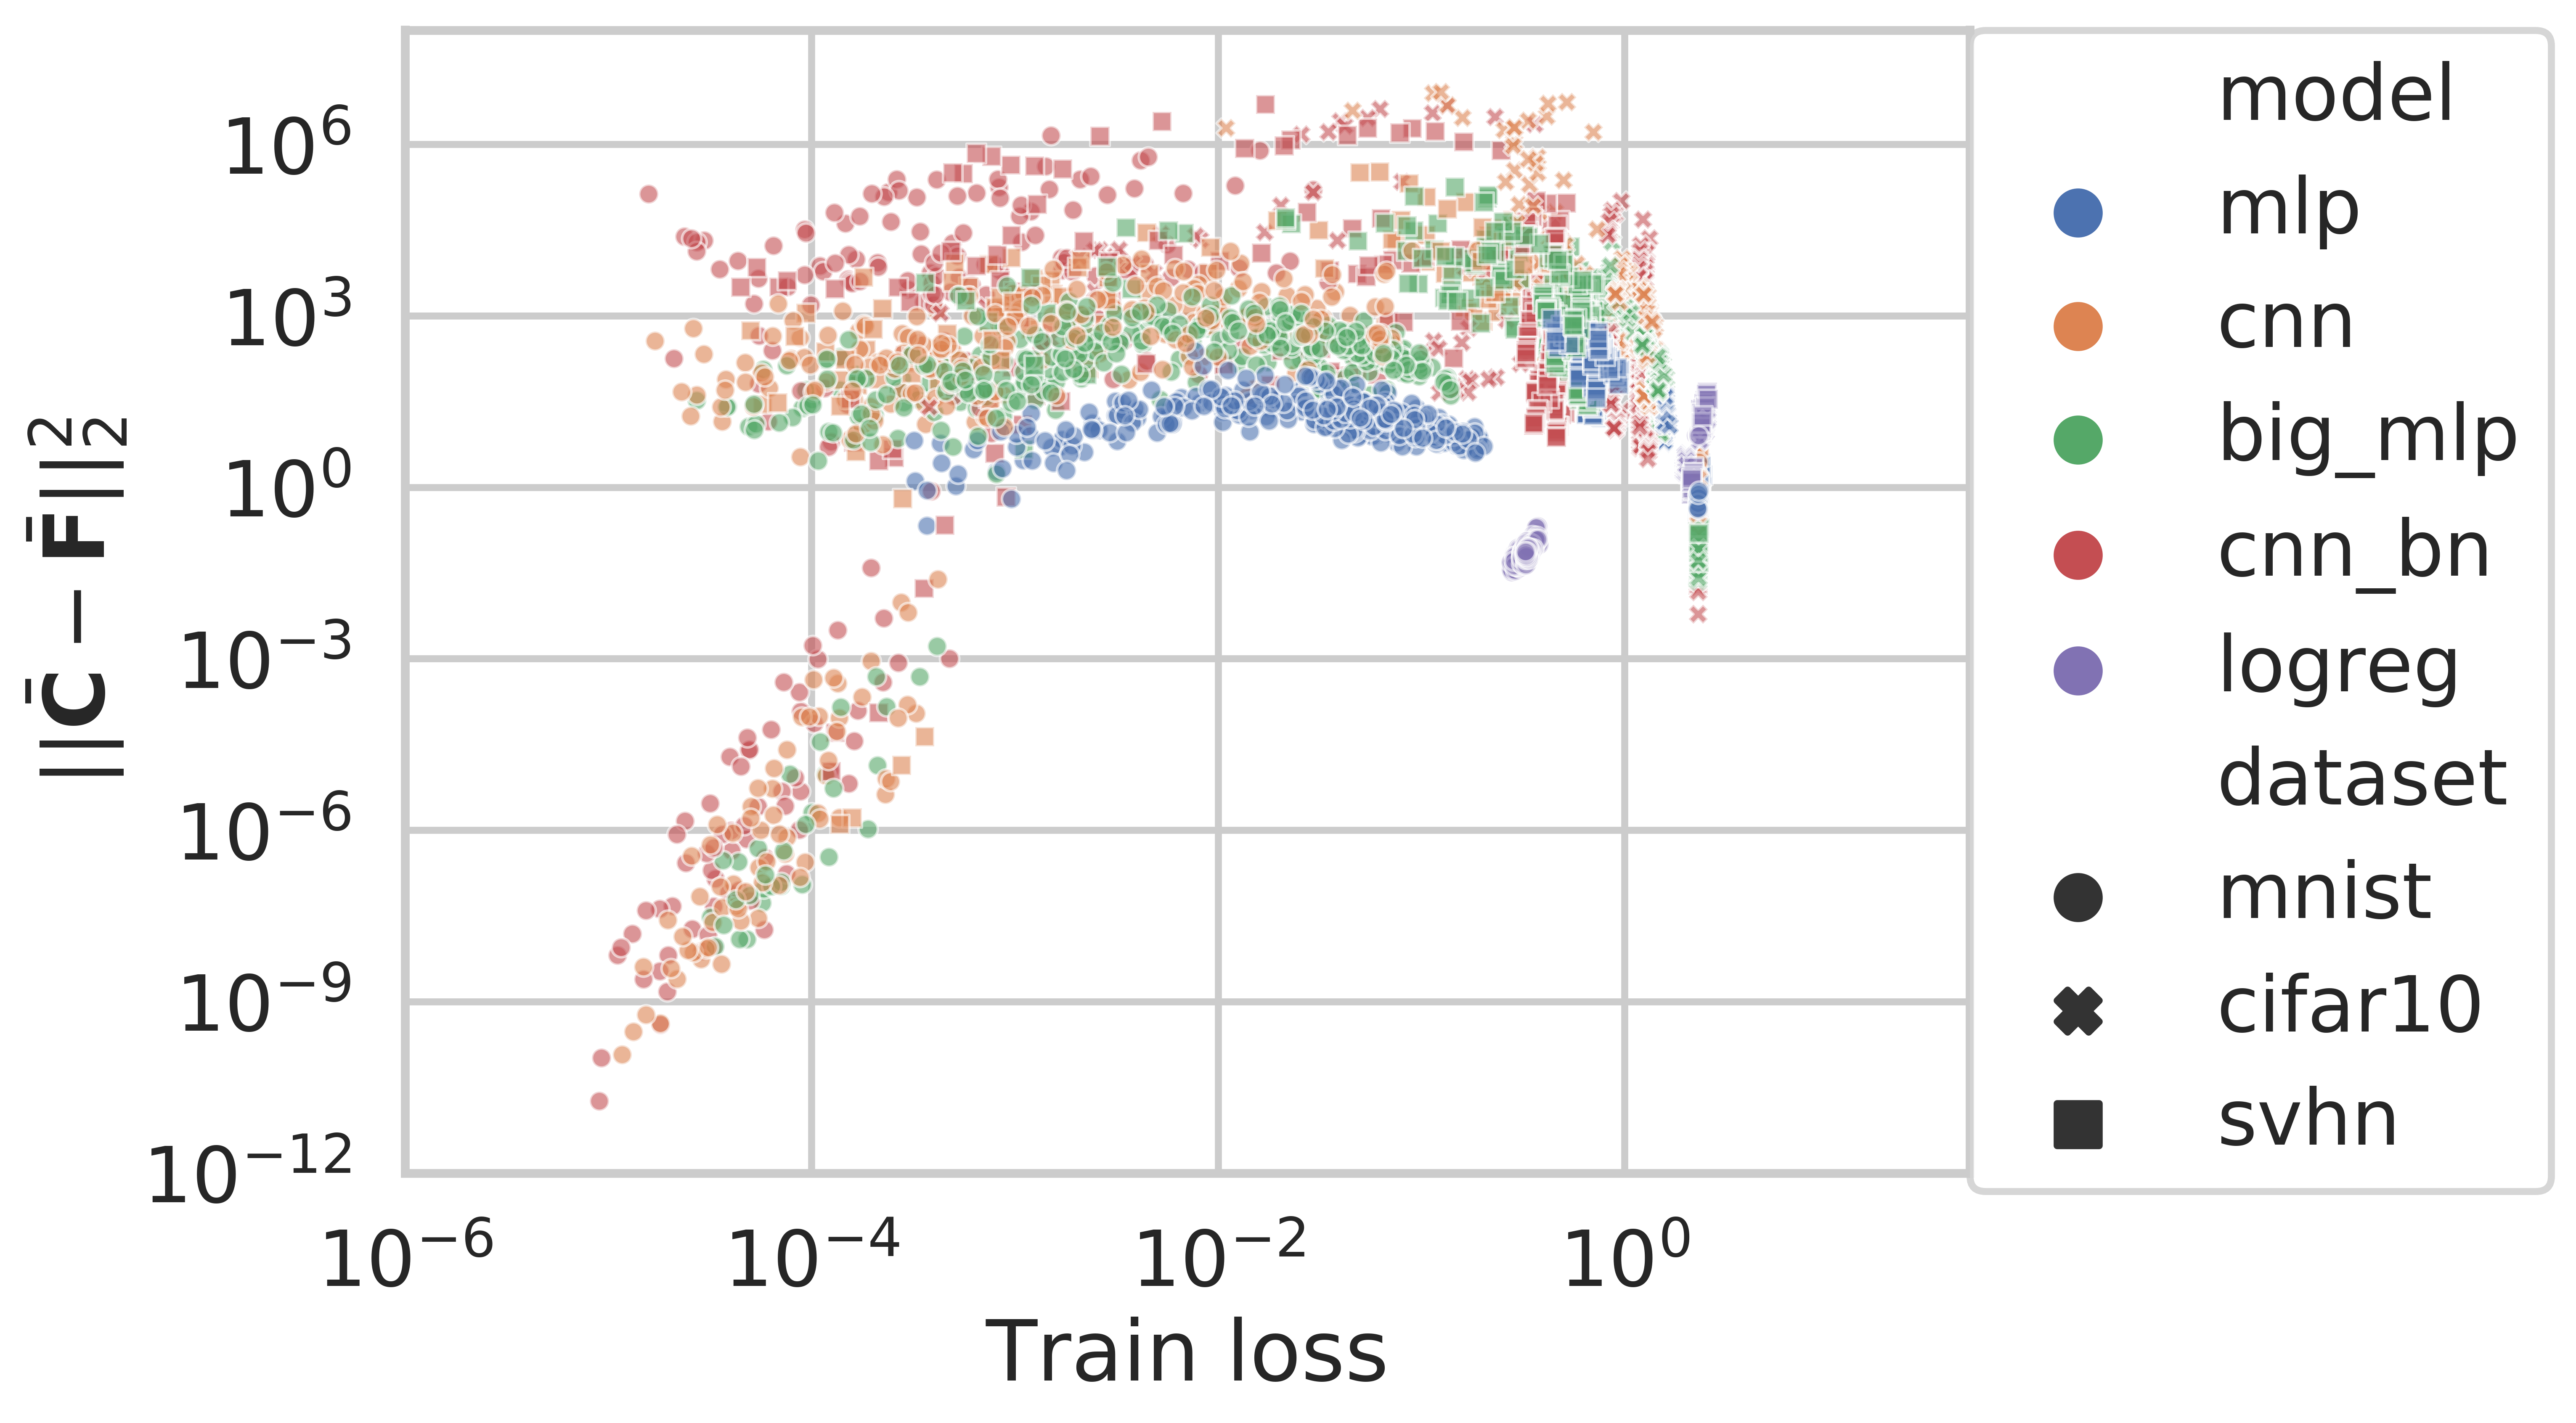
\includegraphics[width=\textwidth]{articles/hfc/FC_train_l2.png}
    \caption{Squared Frobenius norm between $\bar{\rmF}$ and $\bar{\rmC}$ (computed on the training distribution). Even for some low training losses, there can be a significant difference between the two matrices.
    \label{fig:F_vs_C}}
\end{figure}


\subsection{Comparing \texorpdfstring{$\rmH$}{H}, \texorpdfstring{$\rmF$}{F} and \texorpdfstring{$\rmC$}{C}}

\label{sec:HFC_diff}

In this subsection, we analyze the similarities and differences between the information matrices. We will focus on the scale similarity $r$, defined as the ratio of traces, and the angle similarity $s$, defined as the cosine between matrices.
Note that having both $r(\rmA, \rmB) = 1$ and $s(\rmA, \rmB) = 1$ implies $\rmA = \rmB$.

\begin{figure}[ht]

    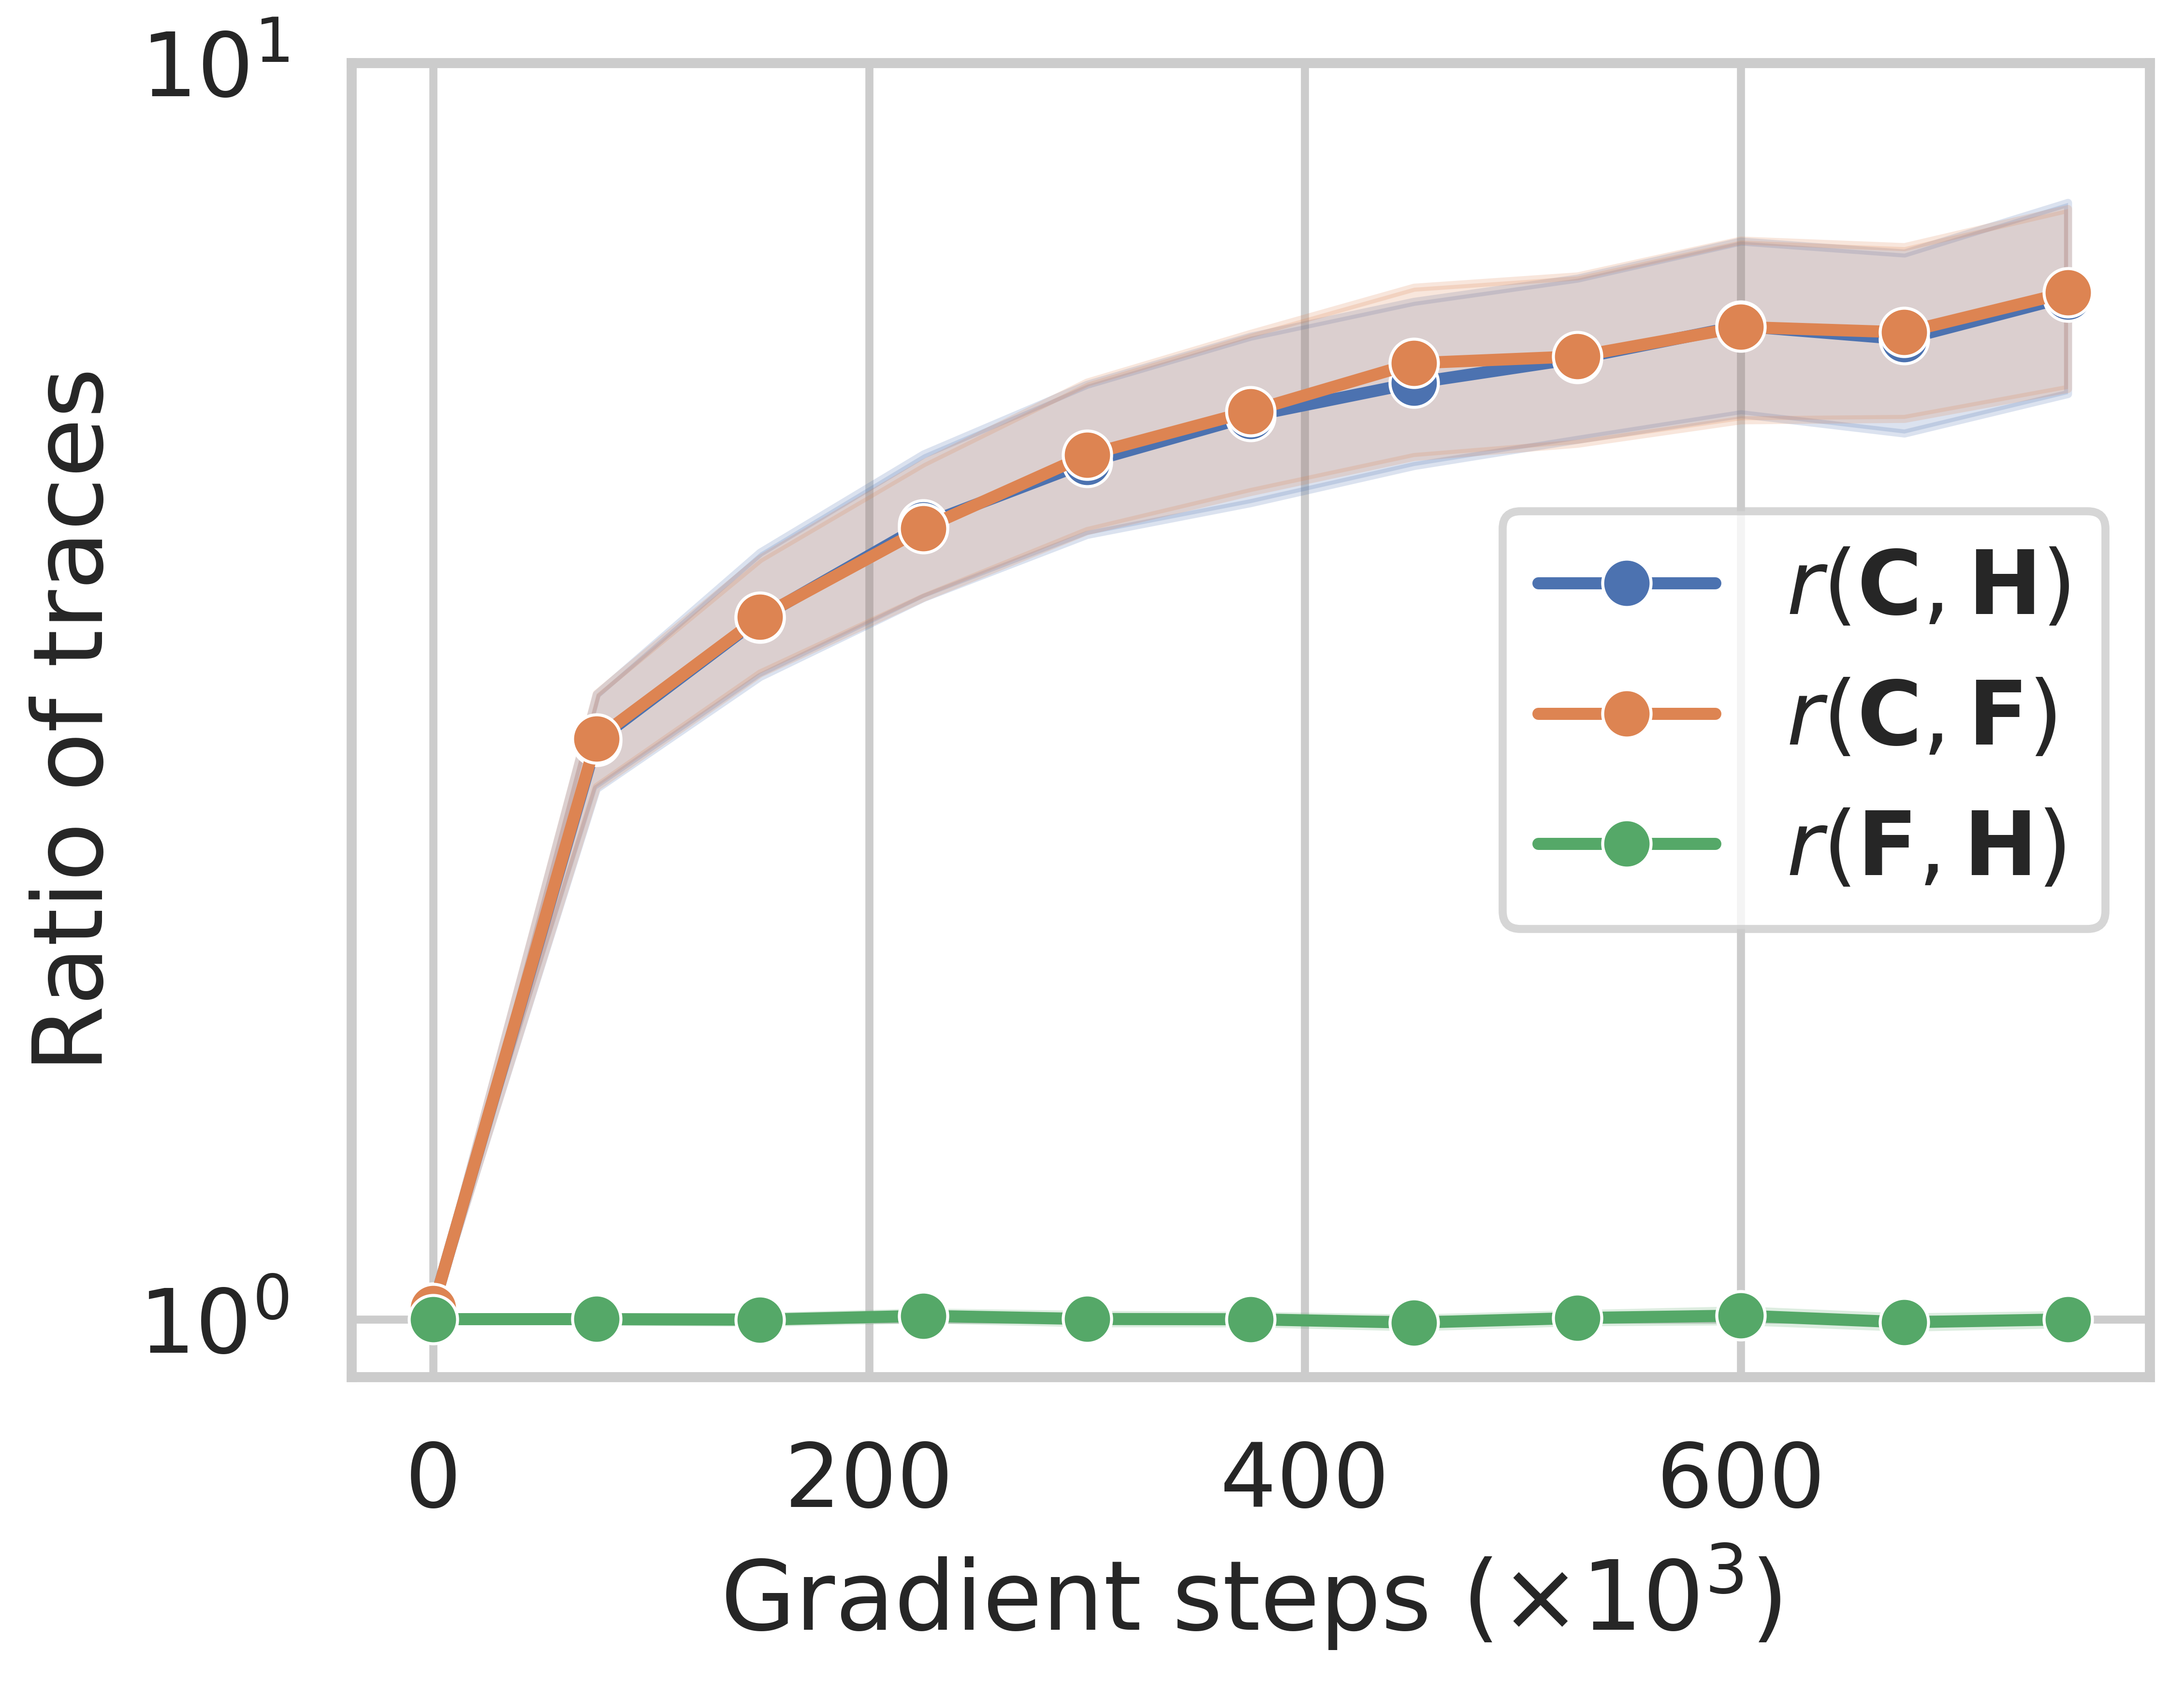
\includegraphics[width=.46\textwidth]{articles/hfc/ratio_trace_HFC_te.png}
      \hfill
    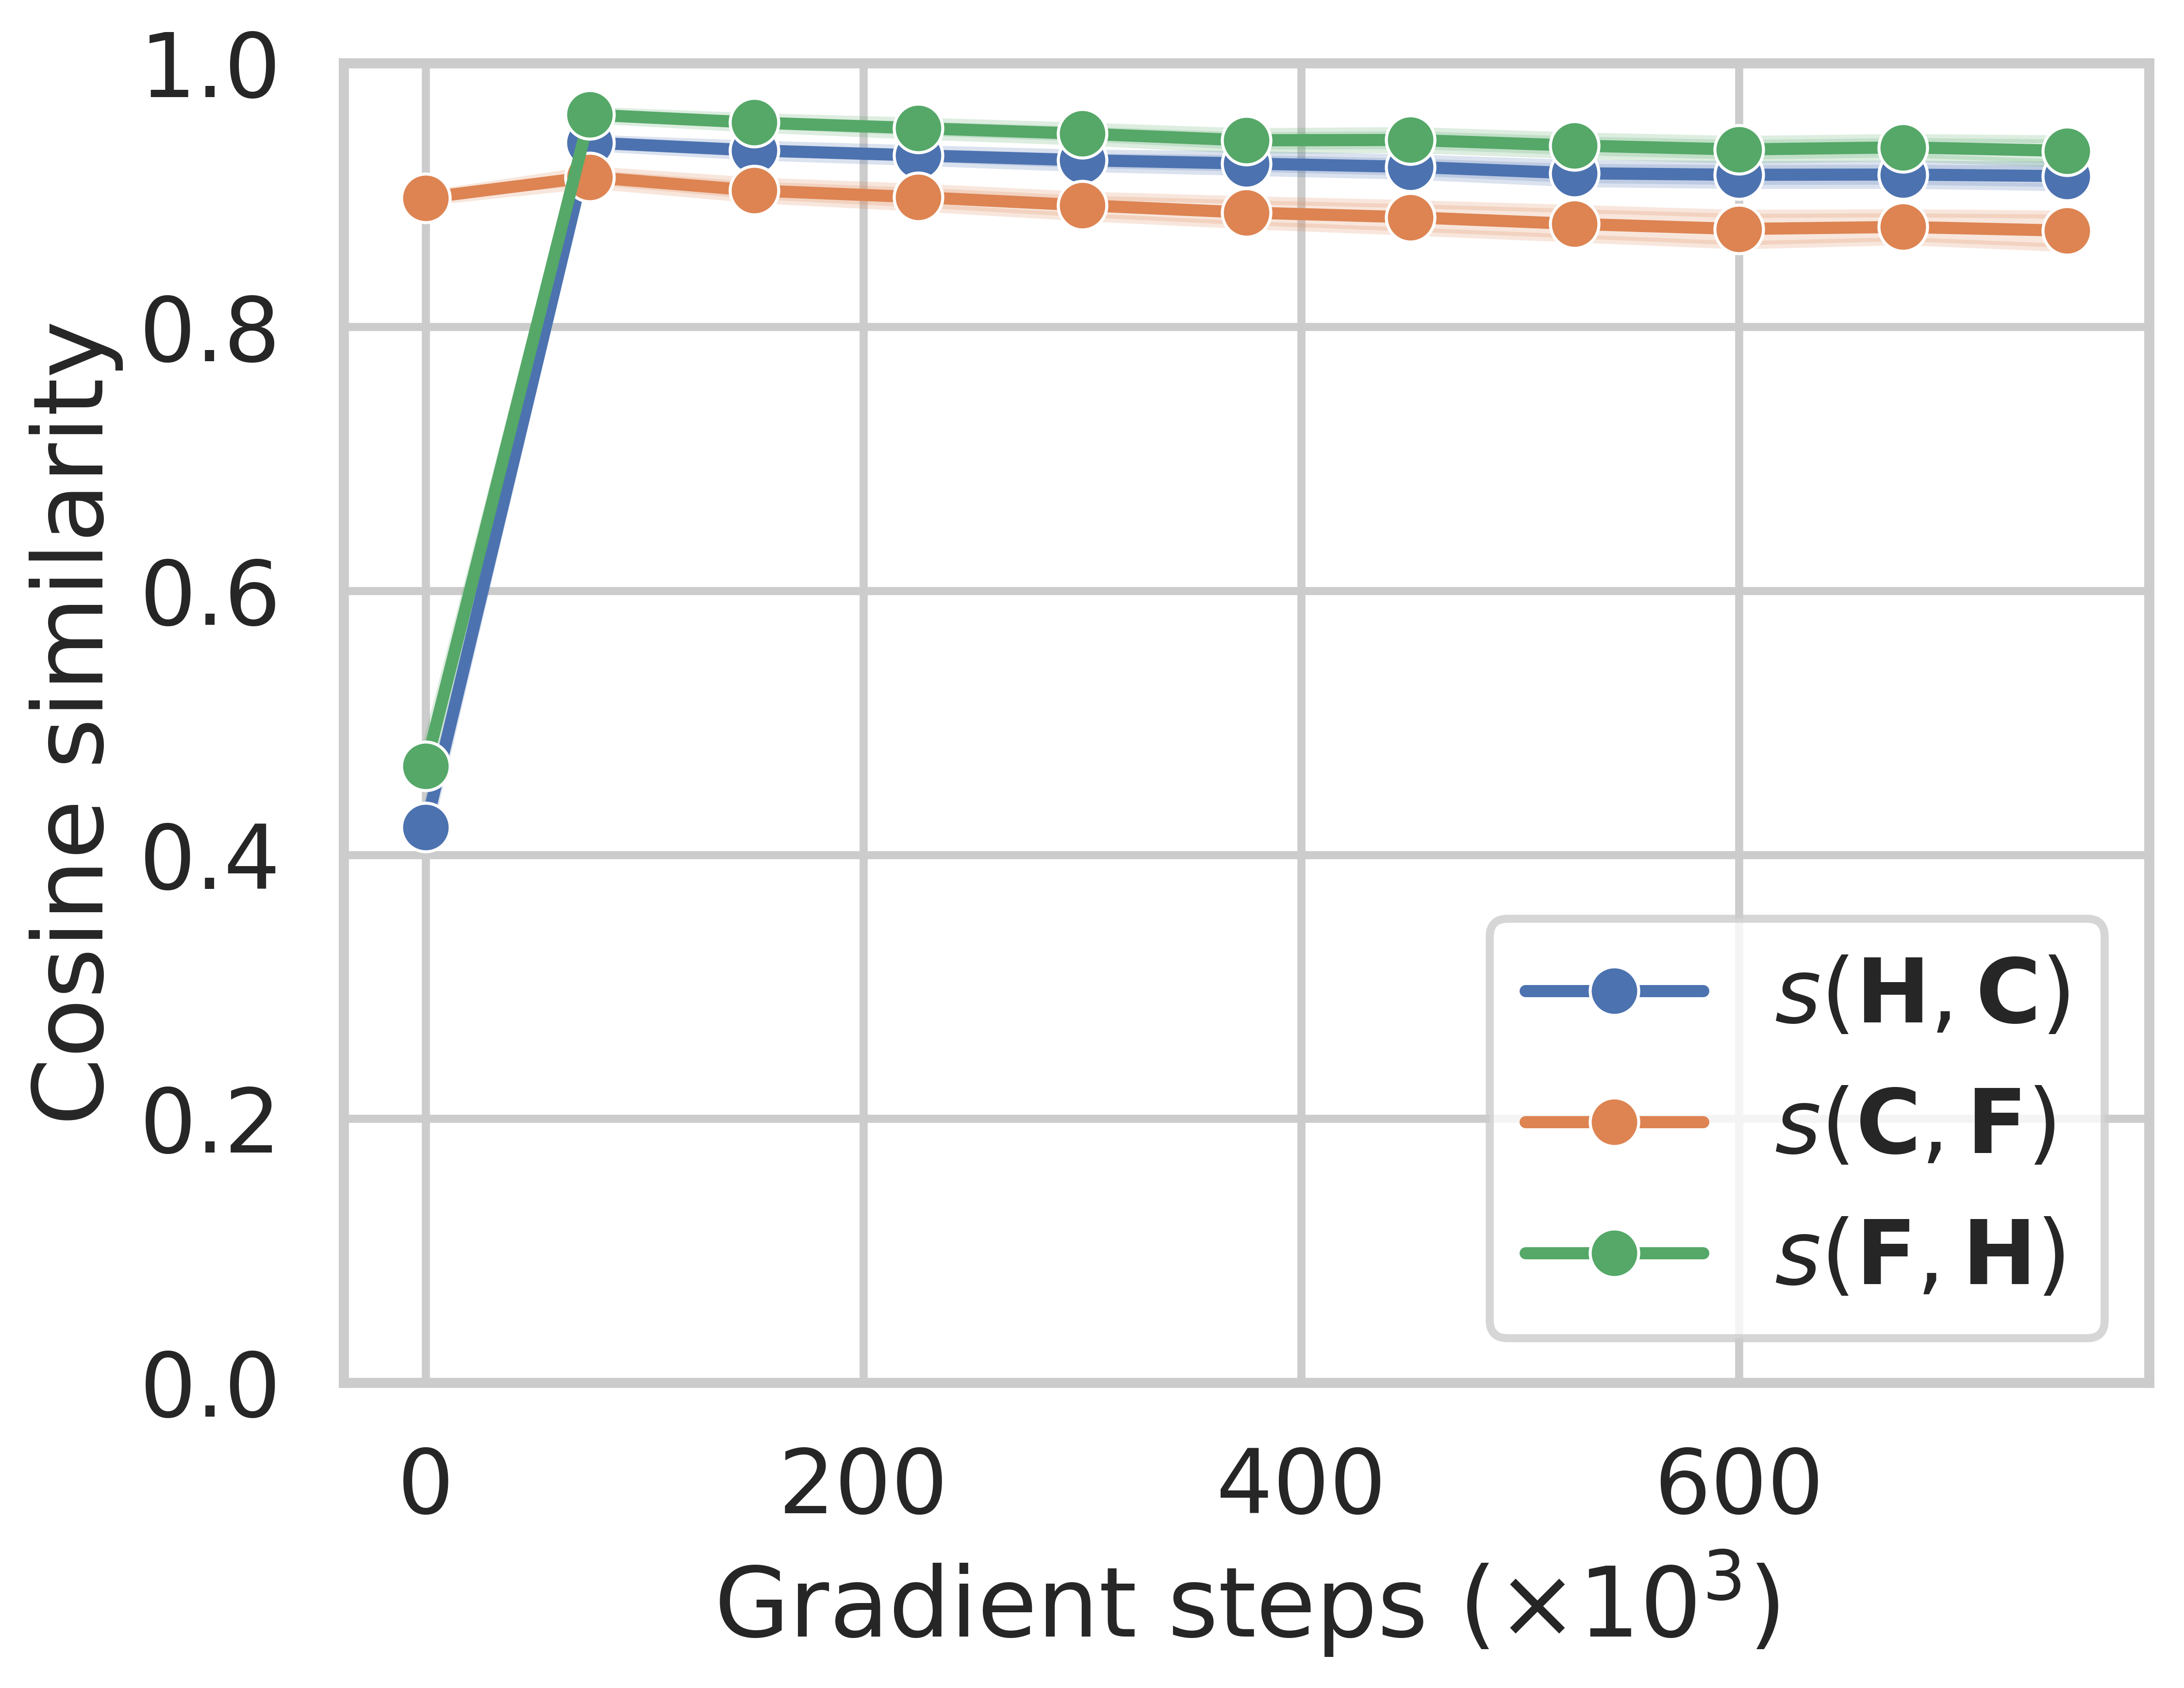
\includegraphics[width=.46\textwidth]{articles/hfc/cossimHFC_te.png}
    \caption{Scale and angle similarities between information matrices.
        \label{fig:similarities}}
\end{figure}

Figure~\ref{fig:similarities} shows the scale (left) and angle (right) similarities between the three pairs of matrices during the optimization of all models used in figure~\ref{fig:large_scale_tic}. We can see that $\rmH$ is not aligned with $\rmC$ nor $\rmF$ at the beginning of the optimization but this changes quickly. Then, all three matrices reach a very high cosine similarity, much higher than we would obtain for two random low-rank matrices. For the scaling, $\rmC$ is ``larger'' than the other two while $\rmF$ and $\rmH$ are very close to each other. Thus, as in the least squares case, we have $\rmC \appropto \rmF \approx \rmH$.

\subsection{Impact of noise on second-order methods}
Section~\ref{sec:optimization} extended existing results to take the geometry of the noise and the curvature into account. Here, we show how the geometry of the noise, and in particular its relationship to the Hessian, can make or break second-order methods in the stochastic setting. To be clear, we assume here that we have access to the full Hessian and do not address the issue of estimating it from noisy samples.

We assume a quadratic $\mathcal{L}(\theta) = \tfrac{1}{2} \theta^\top \rmH \theta$ with $\theta \in \R^{20}$ and $\rmH \in \R^{20\times 20}$ a diagonal matrix such that $\rmH_{ii} = i^2$ with a condition number $d^2 = 400$. At each timestep, we have access to an oracle that outputs a noisy gradient, $\rmH\theta_t + \epsilon$ with $\epsilon$ drawn from a zero-mean Gaussian with covariance $\rmS$. Note here that $\rmS$ is the \emph{centered} covariance of the gradients. We consider three settings: a) $\rmS = \alpha_1 \rmH$; b) $\rmS = \rmI$; c) $\rmS = \alpha_{-1} \rmH^{-1}$ where the constants $\alpha_1$ and $\alpha_{-1}$ are chosen such that $\Tr(\rmS) = d$. Hence, these three settings are indistinguishable from the point of view of the rate of~\citet{schmidt2014convergence}.

In this simplified setting, we get an analytic formula for the variance at each timestep and we can compute the exact number of steps $t$ such that $\E[\Delta_t]$ falls below a suboptimality threshold. To vary the impact of the noise, we compute the number of steps for three different thresholds: a) $\epsilon = 1$; b) $\epsilon = 0.1$; c) $\epsilon = 0.01$. For each algorithm and each noise, the stepsize is optimized to minimize the number of steps required to reach the threshold.

The results are in Table~\ref{tab:iter_noise}. We see that, while Stochastic gradient and momentum are insensitive to the geometry of the noise for small $\epsilon$, Newton method is not and degrades when the noise is large in low curvature directions. For $\epsilon = 10^{-2}$ and $\rmS \propto \rmH^{-1}$, Newton is worse than SG, a phenomenon that is not captured by the bounds of~\citet{bottou2008tradeoffs} since they do not take the structure of the curvature and the noise into account. We also see that the advantage of Polyak momentum over stochastic gradient disappears when the suboptimality is small, i.e. when the noise is large compared to the signal.

Also worthy of notice is the fixed stepsize required to achieve suboptimality $\epsilon$, as shown in Table~\ref{tab:stepsize_noise}. While it hardly depends on the geometry of the noise for SG and Polyak, Newton method requires much smaller stepsizes when $\rmS$ is anticorrelated with $\rmH$ to avoid amplifying the noise.


\begin{table}
\centering
\begin{tabular}{|c|c||c|c|c|}
\hline
$\epsilon$&\textbf{Method} &   $\beta=1$ &   $\beta=0$ &   $\beta=-1$\\
\hline
\multirow{3}{*}{$10^0$}&SG              &   44 &   43 &   42\\
&Newton                                 &   3  &   2   &   19\\
&Polyak                                 &   36  &   36  &   34\\
\hline
\multirow{3}{*}{$10^{-1}$}&SG   &   288     &   253 &   207\\
&Newton                         &   3       &   28  &   225\\
&Polyak                         &   119     &   111 &   97\\
\hline
\multirow{3}{*}{$10^{-2}$}&SG   &   2090    &   1941    &   1731\\
&Newton                         &   29      &   315     &   2663\\
&Polyak                         &   1743    &   1727    &   1705\\
\hline
\end{tabular}
\caption{Number of updates required to reach suboptimality of $\epsilon$ for various methods and $\rmS \propto \rmH^\beta$.
\label{tab:iter_noise}}
\end{table}

\begin{table}
\centering
\begin{tabular}{|c|c||c|c|c|}
\hline
$\epsilon$&\textbf{Method} &   $\beta=1$ &   $\beta=0$ &   $\beta=-1$\\
\hline
\multirow{3}{*}{$10^0$}&SG              &   $5\cdot 10^{-3}$ &   $5\cdot 10^{-3}$ &   $5\cdot 10^{-3}$\\
&Newton                                 &   $1\cdot 10^{0}$  &   $1\cdot 10^0$   &   $2\cdot 10^{-1}$\\
&Polyak                                 &   $5\cdot 10^{-3}$  &   $4\cdot 10^{-3}$  &   $5\cdot 10^{-3}$\\
\hline
\multirow{3}{*}{$10^{-1}$}&SG   &   $4\cdot 10^{-3}$     &   $4\cdot 10^{-3}$ &   $5\cdot 10^{-3}$\\
&Newton                         &   $1\cdot 10^0$       &   $2\cdot 10^0$  & $3\cdot 10^{-2}$\\
&Polyak                         &   $2\cdot 10^{-3}$     &   $2\cdot 10^{-3}$ &   $3\cdot 10^{-3}$\\
\hline
\multirow{3}{*}{$10^{-2}$}&SG   &   $1\cdot 10^{-3}$    &   $1\cdot 10^{-3}$    &   $2\cdot 10^{-3}$\\
&Newton                         &   $2\cdot 10^{-1}$      &   $2\cdot 10^{-2}$     &   $3\cdot 10^{-3}$\\
&Polyak                         &   $3\cdot 10^{-4}$    &   $3\cdot 10^{-4}$    &   $3\cdot 10^{-4}$\\
\hline
\end{tabular}
\caption{Stepsizes achieving suboptimality $\epsilon$ in the fewest updates for various methods and $\rmS \propto \rmH^\beta$.
\label{tab:stepsize_noise}}
\end{table}



\subsection{The TIC and the generalization gap}
\label{sec:neyshabur_gen}
We now empirically test the quality of the TIC as an estimator of the generalization gap in deep networks.
Following~\citet{neyshabur2017exploring} we assess the behaviour of our generalization gap estimator by varying (1) the number of parameters in a model and (2) the label randomization ratio.

Experiments are performed using a fully connected feedforward network with a single hidden layer trained on a subset of $2$k samples of SVHN~\citep{netzer2011reading}. In Figure~\ref{fig:vary_h} we vary the number of units in the hidden layer without label randomization while in Figure~\ref{fig:vary_corr} we vary the label randomization ratio with a fixed architecture.
Each point is computed using 3 different random number generator seeds. The neural networks are trained for 750k steps. The confidence intervals are provided using bootstrapping to estimate a $95 \%$ confidence interval. The Hessian, covariance matrices and sensitivity are computed on a subset of size $5$k of the test data. Details can be found in Appendix~\ref{app:exp_details}.


\begin{figure}[ht]
 \centering
  \begin{subfigure}[b]{.92\textwidth}
    
\includegraphics[trim={0 0 0 2mm},clip, width=\textwidth]{articles/hfc/legend_similarity.png}
  \end{subfigure}
  \centering
  \begin{subfigure}[b]{0.46\textwidth}
    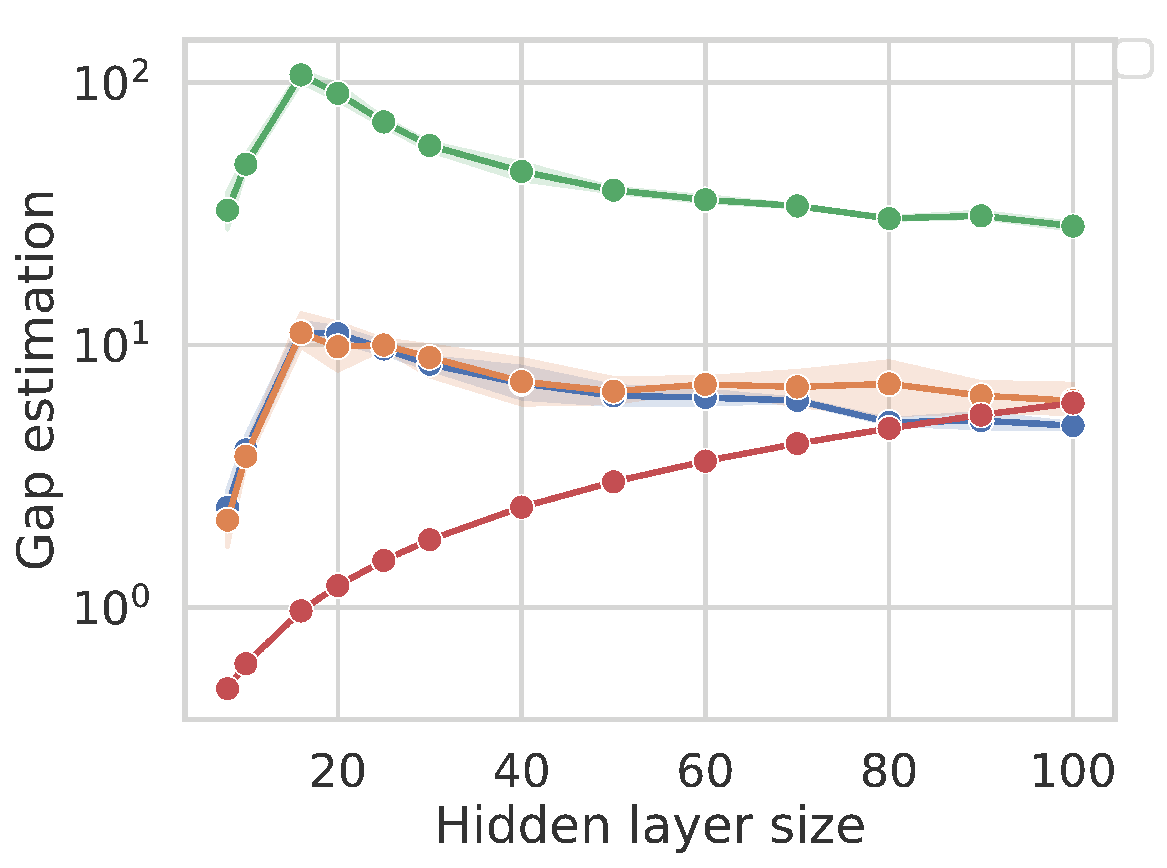
\includegraphics[trim={0 0 8mm 0},clip,width=\textwidth]{articles/hfc/gap_hidden_size_no_lgd-2.pdf}
    \caption{Varying hidden layer size.}
    \label{fig:vary_h}
  \end{subfigure}
  \hfill
  \begin{subfigure}[b]{0.46\textwidth}
    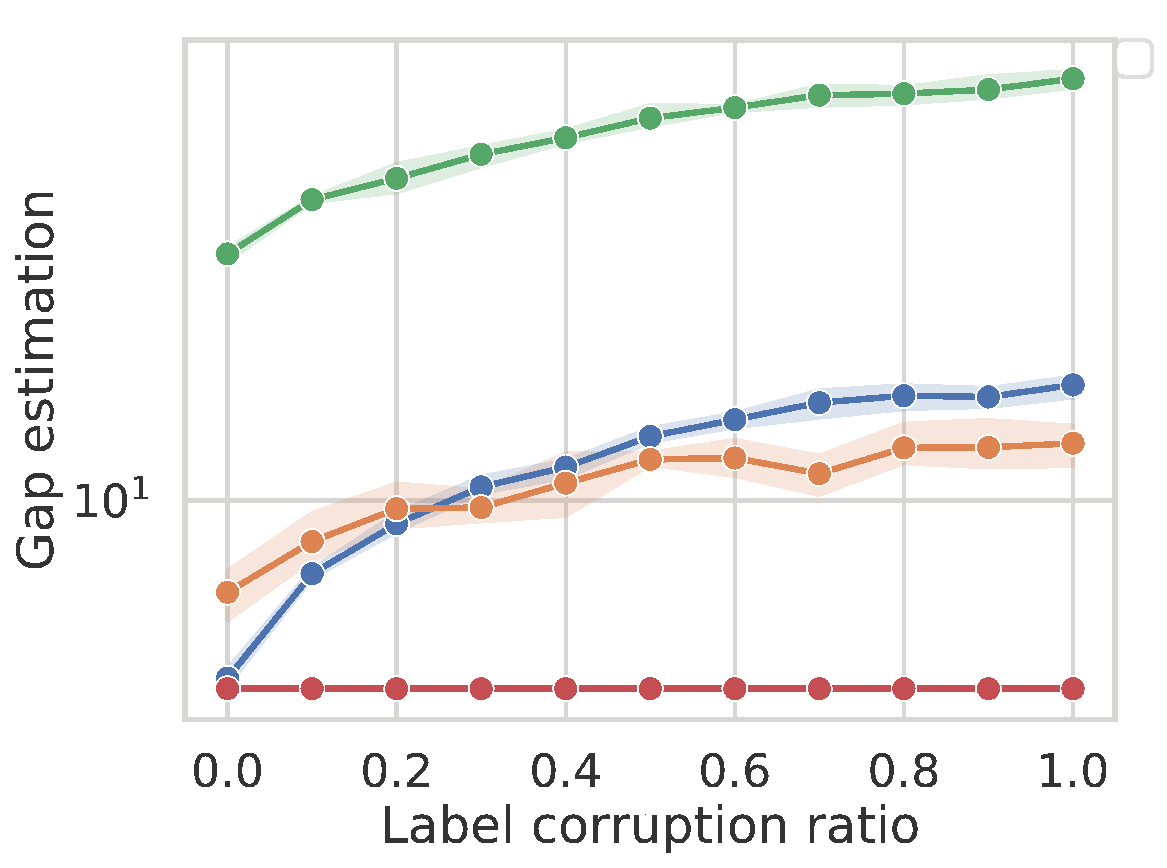
\includegraphics[trim={0 0 8mm 0},clip,width=\textwidth]{articles/hfc/gap_corrupt_no_lgd-2.pdf}
    \caption{Varying the label randomization level.}
    \label{fig:vary_corr}
  \end{subfigure}
 
  \label{fig:neyshabur_exp}
\caption{Comparing the TIC to other estimators of the generalization gap on SVHN. The TIC matches the generalization gap more closely than both the AIC and the sensitivity.}
\end{figure}

We now study the ability of the TIC across a wide variety of models, datasets, and hyperparameters. More specifically, we compare the TIC to the generalization gap for:
The experiments of Figure~\ref{fig:large_scale_tic} are performed with the experimental setup presented in subsection~\ref{sec:exp_setup_hfc}.
Figure~\ref{fig:tic_te} shows that the TIC using $\rmH$ and $\rmC$ computed over the test set is an excellent estimator of the generalization gap. For comparison, we also show in Figure~\ref{fig:flatness} the generalization gap as a function of $\rmH$ computed over the test set. We see that, even when using the test set, the correlation is much weaker than with the TIC.
\begin{figure}[ht]
\centering
\begin{subfigure}[b]{.92\textwidth}
    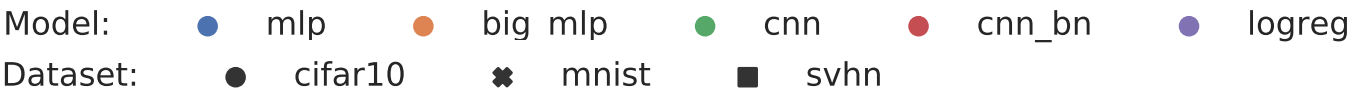
\includegraphics[trim={0mm 0mm 0mm 0mm},clip,width=\textwidth]{articles/hfc/legend_gimp.png}
  \end{subfigure}
  \centering
  \begin{subfigure}[b]{0.46\textwidth}
    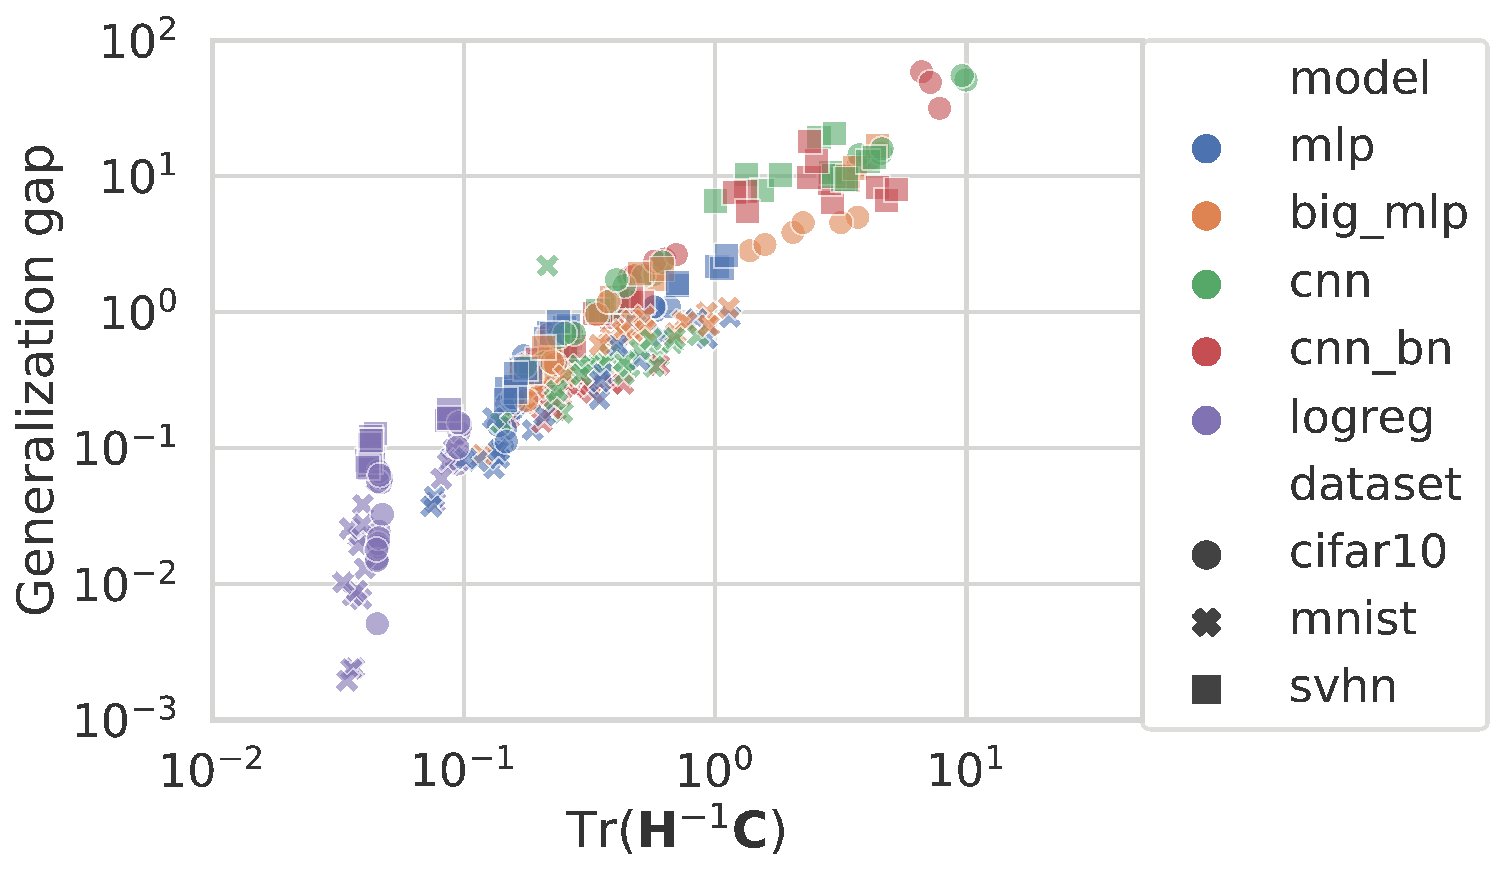
\includegraphics[trim={0 0 60mm 0},clip,width=\textwidth]{articles/hfc/trhic750-2.pdf}
    \caption{ Gap vs. TIC.
    \label{fig:tic_te}}
  \end{subfigure}
    \hfill
      \begin{subfigure}[b]{0.46\textwidth}
    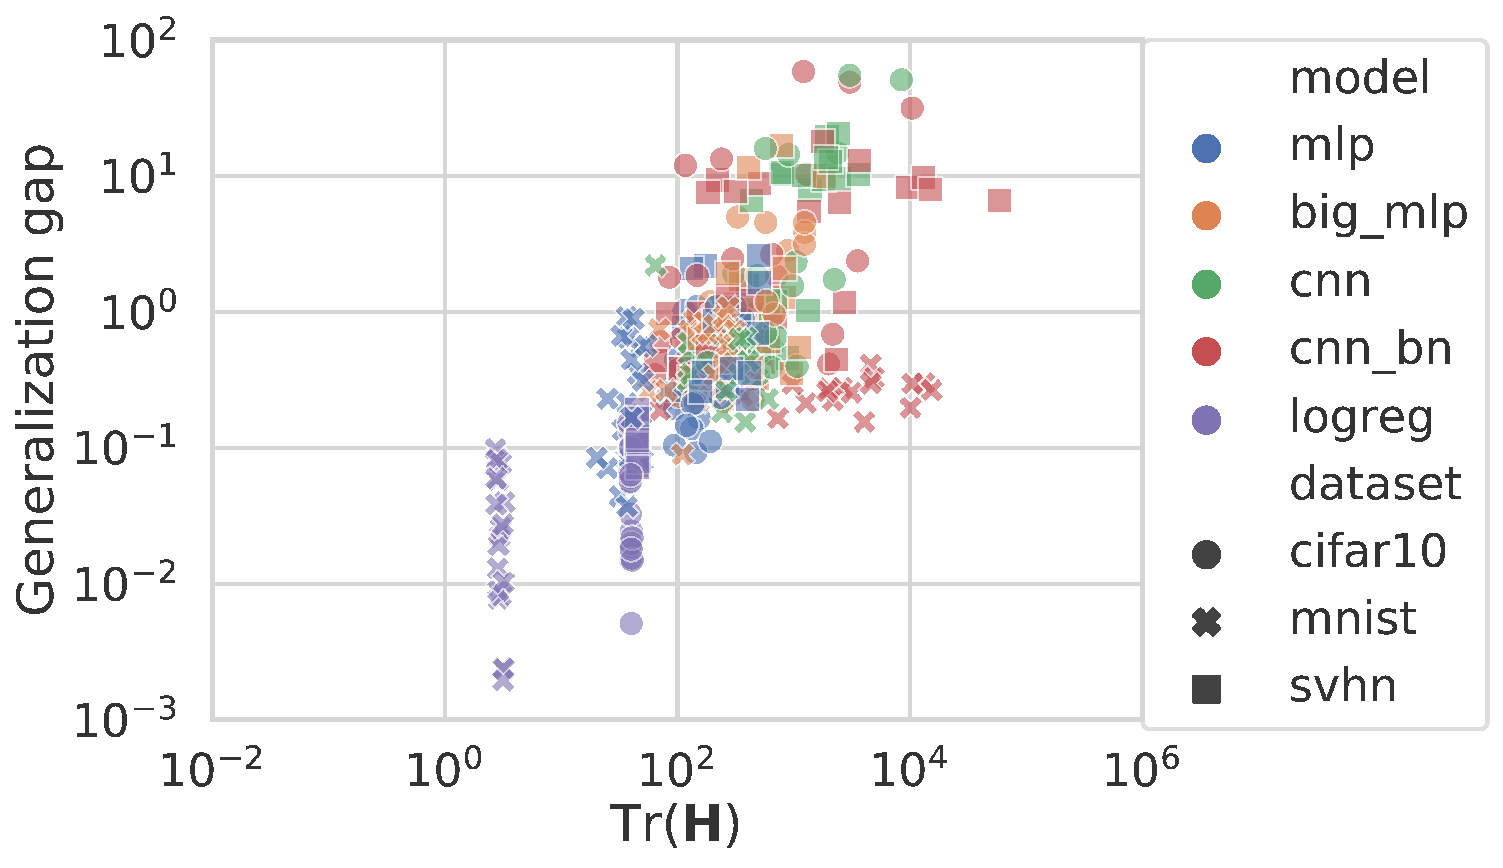
\includegraphics[trim={0 0 55mm 0},clip,width=\textwidth]{articles/hfc/trh750_te-2.pdf}
    \caption{ Gap vs. flatness.
    \label{fig:flatness}}
  \end{subfigure}
  
      \caption{Generalization gap as a function of the Takeuchi information criterion (\emph{left}) and the trace of the Hessian on the test set (\emph{right}) for many architectures, datasets, and hyperparameters. Correlation is perfect if all points lie on a line. We see that the Hessian cannot by itself capture the generalization gap.}
      \label{fig:large_scale_tic}
\end{figure}




\subsubsection{Efficient approximations to the TIC}
\label{sec:tic_approx}
Although the TIC is a good estimate of the generalization gap, it can be expensive to compute on large models. Following our theoretical and empirical analysis of the proximity of $\rmH$ and $\rmF$, we propose two approximations to the TIC: $\Tr(\rmF^{-1} \rmC)$ and $\Tr(\rmC) / \Tr(\rmF)$. They are easier to compute as the $\rmF$ is in general easier to compute than $\rmH$ and the second does not require any matrix inversion.


\begin{figure}[ht]
\centering
    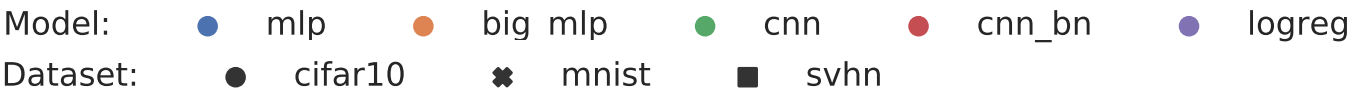
\includegraphics[trim={00mm 0mm 0mm 0mm},clip,width=.8\textwidth]{articles/hfc/legend_gimp.png}
    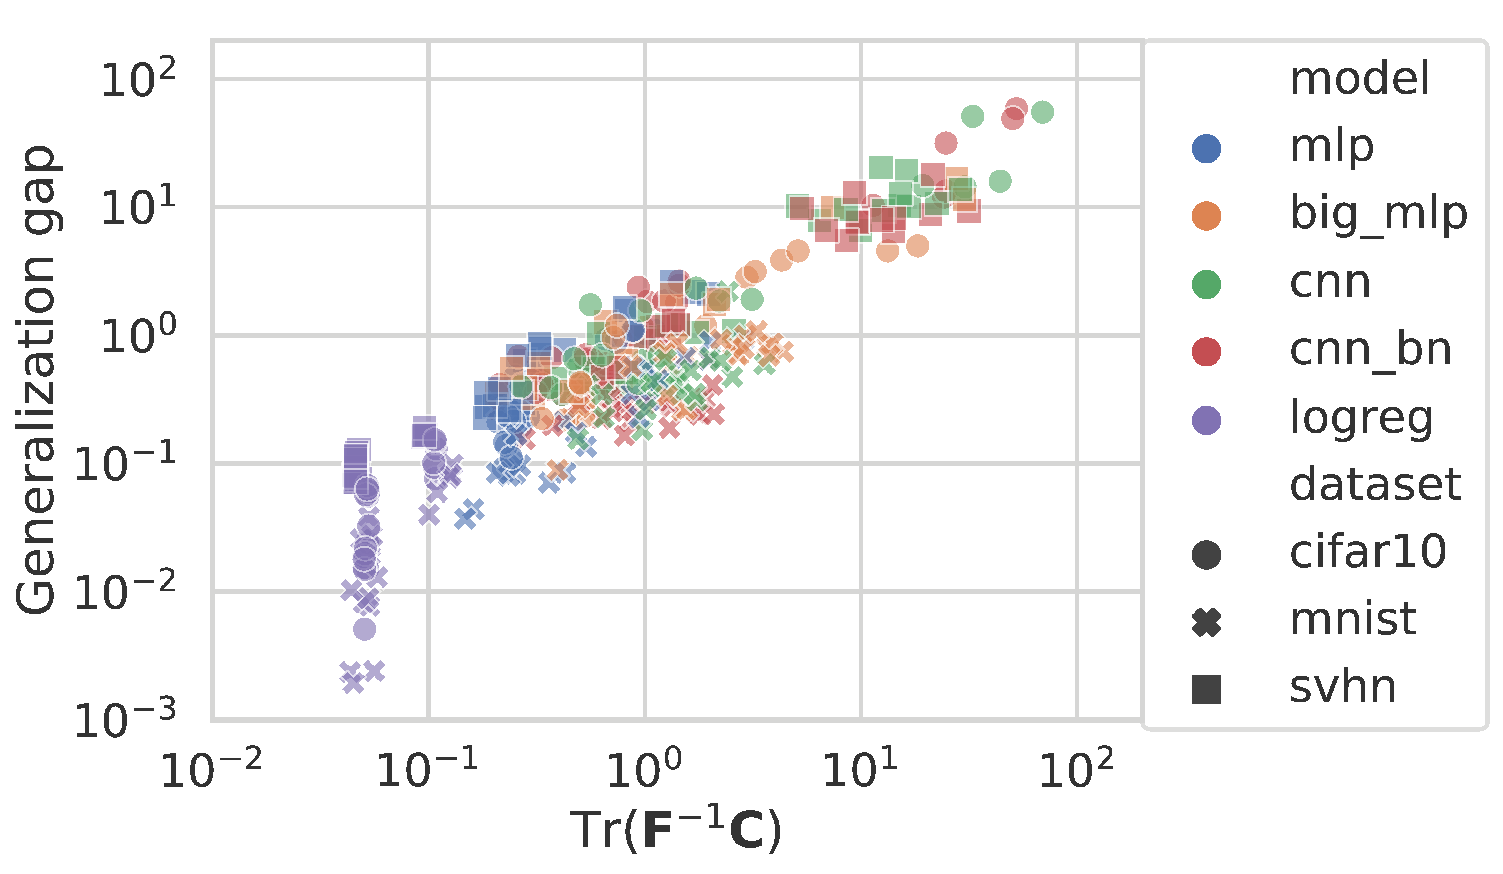
\includegraphics[trim={0 0 60mm 0},clip,width=.46\textwidth]{articles/hfc/trfic750-2.pdf}
    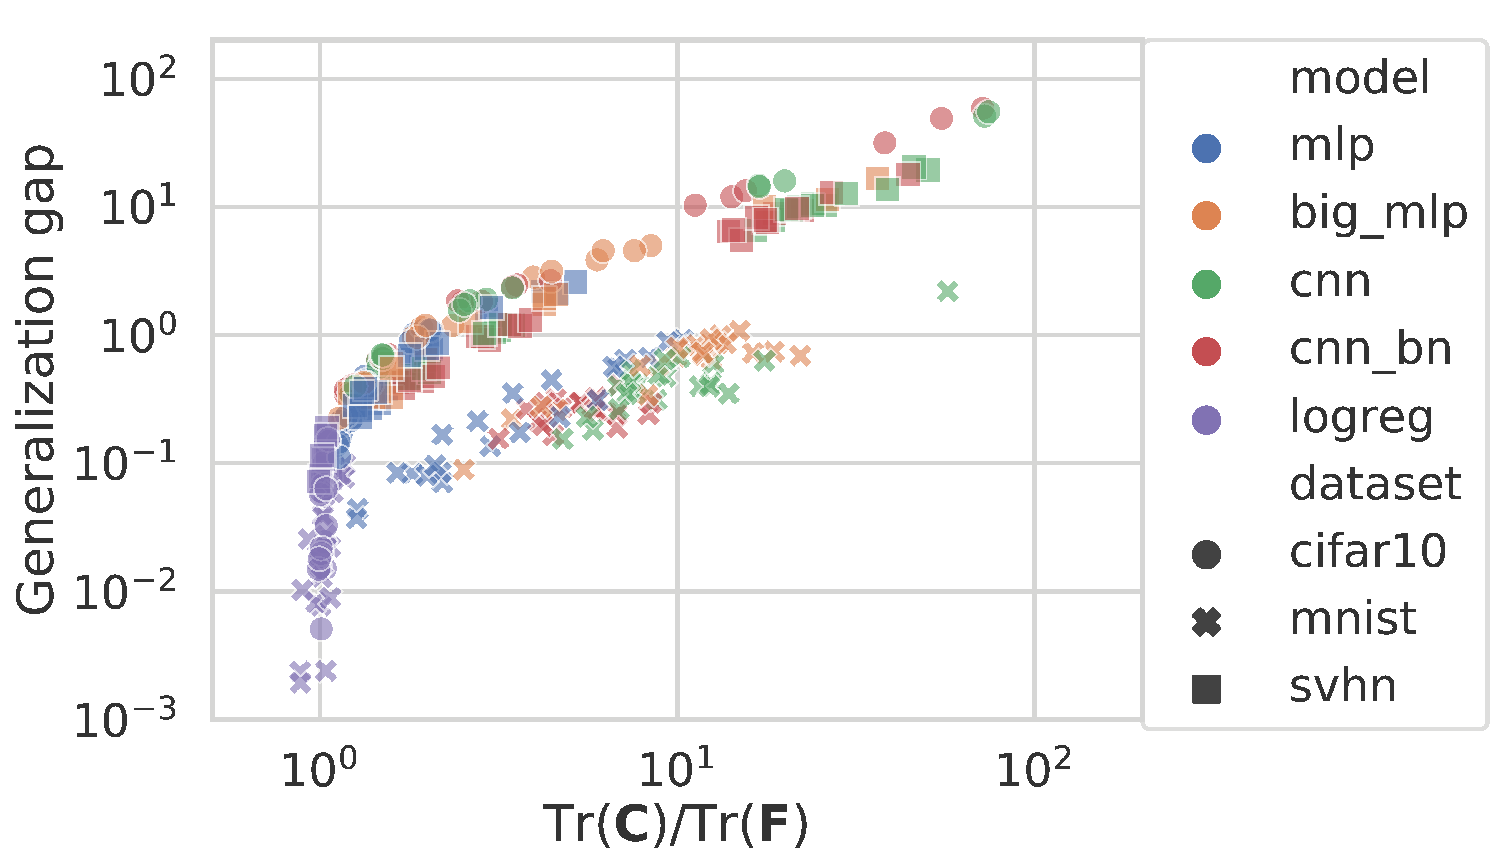
\includegraphics[trim={0 0 60mm 0},clip,width=.46\textwidth]{articles/hfc/ratiotrcof750-2.pdf}
\caption{Generalization gap as a function of two approximations to the Takeuchi Information Criterion: $\Tr(\rmF^{-1} \rmC)$ (\emph{left}) and $\Tr(\rmC) / \Tr(\rmF)$ (\emph{right}).
\label{fig:tic_approx}}
\end{figure}


Using the same experimental setting as in~\ref{sec:neyshabur_gen}, we observe in Figure~\ref{fig:tic_approx} that the replacing $\rmH$ with $\rmF$ leads to almost no loss in predictive performance. On the other hand, the ratio of the traces works best when the generalization gap is high and tends to overestimate it when it is small.

\textbf{Intuition on $\Tr(\rmC) / \Tr(\rmF)$}: it is not clear right away why the ratio of traces might be a interesting quantity. However, as observed in figure~\ref{fig:similarities}, $\rmC$ and $\rmF$ are remarkably aligned, but there remains a scaling factor. If we had $\rmC = \alpha \rmF$, then $\Tr(\rmF^{-1} \rmC) = k \alpha$ where $k$ is the dimension of the invertible subspace of $\rmF$ and $\Tr(\rmC) / \Tr(\rmF) = d \alpha$ where $d$ is the dimensionality of $\theta$. So, up to a multiplicative constant (or an offset in log scale), we can expect these two quantities to exhibit similarities.
Notice that on figure~\ref{fig:tic_approx}, this offset does appear and is different for every dataset (MNIST has the smallest one, then SVHN and CIFAR10, just slightly bigger).

\subsection{The importance of the noise in estimating the generalization gap}
For a given model, the generalization gap captures the discrepancy that exists between the training set and the data distribution. Hence, estimating that gap involves the evaluation of the uncertainty around the data distribution. The TIC uses $\rmC$ to capture that uncertainty but other measures probably exist. However, estimators which do not estimate it are bound to have failure modes. For instance, by using the square norm of the derivative of the loss with respect to the input, the sensitivity implicitly assumes that the uncertainty around the inputs is isotropic and will fail should the data be heavily concentrated in a low-dimensional subspace. It would be interesting to adapt the sensitivity to take the covariance of the inputs into account.

Another aspect worth mentioning is that estimators such as the margin assume that the classifier is fixed but the data is a random variable. Then, the margin quantifies the probability that a new datapoint would fall on the other side of the decision boundary. By contrast, the TIC assumes that the data are fixed but that the classifier is a random variable. It estimates the probability that a classifier trained on slightly different data would classify a training point incorrectly. In that, it echoes the uniform stability theory~\citep{bousquet2002stability}, where a full training with a slightly different training set has been replaced with a local search.








\section{Conclusion and open questions}
We clarified the relationship between information matrices used in optimization. While their differences seem obvious in retrospect, the widespread confusion makes these messages necessary. Indeed, several well-known algorithms, such as Adam~\citep{kingma2014adam}, claiming to use second-order information about the loss to accelerate training seem instead to be using the covariance matrix of the gradients. Equipped with this new understanding of the difference between the curvature and noise information matrices, one might wonder if the success of these methods is not due to variance reduction instead. If so, one should be able to combine variance reduction and geometry adaptation, an idea attempted by~\citet{leroux2011}.

We also showed how, in certain settings, the geometry of the noise could affect the performance of second-order methods. While Polyak momentum is affected by the scale of the noise, its performance is independent of the geometry, similar to stochastic gradient but unlike Newton method. However, empirical results indicate that common loss functions are in the regime favorable to second-order methods.

Finally, we investigated whether the Takeuchi information criterion is relevant for estimating the generalization gap in neural networks. We provided evidence that this complexity measures involving the information matrices is predictive of the generalization performance.

We hope this study will clarify the interplay of the noise and curvature in common machine learning settings, potentially giving rise to new optimization algorithms as well as new methods to estimate the generalization gap.

\subsubsection*{Acknowledgments}
We would like to thank Gauthier Gidel, Reyhane Askari and Giancarlo Kerg for reviewing an earlier version of this paper. We also thank Aristide Baratin for insightful discussions.
Valentin Thomas acknowledges funding from the Open Philantropy project.






\chapter{Beyond Variance Reduction: Understanding the True Impact of Baselines on Policy Optimization}
\label{chapter:baselines}
\section*{Article details}
Thomas V*, Chung W*, Machado M. C., Le Roux N. ``Beyond variance reduction: Understanding the true impact of baselines on policy optimization''. In \emph{International Conference on Machine Learning (ICML) 2021. PMLR}.

\section*{Foreword}
In the summer of 2019, I interned at Google Brain Montr\'{e}al with Nicolas Le Roux and Marlos C. Machado and my project was initially about using off-policy learning to reduce the variance of the gradients for Policy Gradient methods in Reinforcement Learning. However, when comparing our method to other variance reduction methods, such as the use of baselines, I came to realise that \emph{symmetric} perturbations of the variance-minimizing baseline (e.g $\pm \epsilon$), while increasing the variance by the same amount, led to \emph{asymmetric} impacts on the regret/average reward. While we initially decided to continue exploring the first project, we came back to this observation which Wesley had begun to work on with Nicolas. By studying this on simple examples such as a two-arm bandits, Nicolas was first able to demonstrate our first divergence result. During the year 2020, we worked together on extending both the divergence and convergence results and deepened our understanding of the problem.

This paper could be described as one pointing out a surprising flaw in a widely used algorithm and as such it inspired future work. The most relevant direct line of work inspired by our article is the one led by Jincheng Mei who worked previously on the convergence of policy gradient methods in the \emph{expected} regime. 

\section*{Impact since publication}
Following our work, \citet{mei2021understanding} extended our observation to a vast class of algorithms: those which are too greedy, or \emph{committal} and may converge prematurely to a suboptimal solution. Finally, we (Jincheng, Wesley and I) started collaborating together and this culminated in a paper \emph{The Role of Baselines in Policy Optimization}~\citep{mei2022role} published at NeurIPS 2022 which sheds light on how baselines impact the exploration behavior of policy gradient methods and how using the value function as a baseline guarantees policy improvement in expectation while the variance-minimizing baseline may not. As such policy gradient using the true value function as a baseline can converge to the optimal policy fast.


\section*{Personal contribution}
\begin{itemize}
    \item The original observation that baselines impact not only the variance but also the convergence of Policy Gradient methods was done by me during my summer internship at Google Brain with Nicolas and Marlos
    \item Theory (convergence proofs) and experiments for the off-policy setting with the collaboration of Wesley for the extension to $K > 2$ arms
    \item Collaboration with Wesley on the divergence proofs for the 3 arms setting
    \item Design of the simplex visualizations (\Cref{fig:trajectories} and \Cref{fig:simplex_variance})
    \item Writing of the paper alongside with all my co-authors
\end{itemize}



\begin{abstract}


Bandit and reinforcement learning (RL) problems can often be framed as optimization problems where the goal is to maximize average performance while having access only to stochastic estimates of the true gradient. Traditionally, stochastic optimization theory predicts that learning dynamics are governed by the curvature of the loss function and the noise of the gradient estimates. In this paper we demonstrate that the standard view is too limited for bandit and RL problems. To allow our analysis to be interpreted in light of multi-step MDPs, we focus on techniques derived from stochastic optimization principles~(e.g., natural policy gradient and EXP3) and we show that some standard assumptions from optimization theory are violated in these problems. We present theoretical results showing that, at least for bandit problems, curvature and noise are not sufficient to explain the learning dynamics and that seemingly innocuous choices like the baseline can determine whether an algorithm converges. These theoretical findings match our empirical evaluation, which we extend to multi-state MDPs.
\end{abstract}

\section{Introduction}
In the standard multi-arm bandit setting~\cite{robbins1952some}, an agent needs to choose, at each timestep $t$, an arm $a_t \in \{1, ..., n\}$ to play, receiving a potentially stochastic reward $r_t$ with mean $\mu_{a_t}$. The goal of the agent is usually to maximize the total sum of rewards, $\sum_{i=1}^T r_i$, or to maximize the average performance at time $T$, $\E_{i\sim \pi} \mu_i$ with $\pi$ being the probability of the agent of drawing each arm~\citep{bubeck2012regret}. While the former measure is often used in the context of bandits,\footnote{The objective is usually presented as regret minimization.} $\E_{i\sim \pi} \mu_i$ is more common in the context of Markov Decision Processes (MDPs), which have multi-arm bandits as a special case.

In this paper we focus on techniques derived from stochastic optimization principles, such as EXP3~\citep{auer2002nonstochastic, seldin2013evaluation}. %
In particular, we study \textit{policy gradient} methods, a family of algorithms useful in the more general MDP setting which have seen empirical success in recent times \cite{schulman2017proximal}. 


We analyze the problem of learning to maximize the average reward, $\gJ$, by gradient ascent:
\begin{align}
    \theta^\ast &= \arg\max_\theta \gJ(\theta)
    = \arg\max_\theta \sum_{a} \pi_\theta(a) \mu_a \; , \label{eq:bandit_loss} 
\end{align} 
with $\mu_a$ being the average reward of arm $a$.
In this case, we are mainly interested in outputting an effective policy at the end of the optimization process, without explicitly considering the performance of intermediary policies.%


Optimization theory predicts that the convergence speed of stochastic gradient methods will be affected by the variance of the gradient estimates and by the geometry of the function $\gJ$, represented by its curvature. Roughly speaking, the geometry dictates how effective true gradient ascent is at optimizing $\gJ(\theta)$ while the variance can be viewed as a penalty, capturing how much slower the optimization process is by using noisy versions of this true gradient. More concretely, doing one gradient step with stepsize $\alpha$, using a stochastic estimate $g_t$ of the gradient, leads to \citep{bottou2018optimization}:
\begin{align*}\E[\gJ(\theta_{t+1})] - \gJ(\theta_t) &\geq (\alpha - \tfrac{L \alpha^2}{2}) \|\E [g_t] \|^2_2  - \tfrac{ L \alpha^2}{2} \text{Var}[g_t ],\end{align*}
when $\gJ$ is $L$-smooth, i.e. its gradients are $L$-Lipschitz. 

As large variance has been identified as an issue for policy gradient (PG) methods, many works have focused on reducing the noise of the updates. One common technique is the use of control variates~\citep{greensmith2004variance, hofmann2015variance}, referred to as \emph{baselines} in the context of RL. These baselines $b$ are subtracted from the observed returns to obtain shifted returns, $r(a_i) - b$, and do not change the expectation of the gradient. In MDPs, they are typically state-dependent.
While the value function is a common choice, previous work showed that the minimum-variance baseline for the REINFORCE \citep{williams1992simple} estimator is different and involves the norm of the gradient~\citep{peters2008reinforcement}.
Reducing variance has been the main motivation for many previous works on baselines~\citep[e.g.,][]{gu2016q, liu2017action, grathwohl2017backpropagation, wu2018variance, cheng2020trajectory}, but the influence of baselines on other aspects of the optimization process has hardly been studied. We take a deeper look at baselines and their effects on optimization.

\subsubsection*{Contributions}
We show that baselines can impact the optimization process 
beyond variance reduction and lead to qualitatively different learning curves, even when the variance of the gradients is the same. 
For instance, given two baselines with the same variance, the more negative baseline promotes \textit{committal} behaviour where a policy quickly tends towards a deterministic one, while the more positive baseline leads to \textit{non-committal} behaviour, where the policy retains higher entropy for a longer period.

Furthermore, we show that \textbf{the choice of baseline can even impact the convergence of natural policy gradient} (NPG), something variance cannot explain. In particular, we construct a three-armed bandit where using the baseline minimizing the variance can lead to convergence to a deterministic, sub-optimal policy for any positive stepsize, while another baseline, with larger variance, guarantees convergence to the optimal policy. As such a behaviour is impossible under the standard assumptions in optimization, this result shows how these assumptions may be violated in practice. It also provides a counterexample to the convergence of NPG algorithms in general, a popular variant with much faster convergence rates than vanilla PG when using the true gradient in tabular MDPs~\citep{agarwal2019optimality}. 

Further, \textbf{we identify on-policy sampling as a key factor to these convergence issues} as it induces a vicious cycle where making bad updates can lead to worse policies, in turn leading to worse updates. A natural solution is to break the dependency between the sampling distribution and the updates through off-policy sampling. We show that ensuring all actions are sampled with sufficiently large probability at each step is enough to guarantee convergence in probability. Note that this form of convergence is stronger than convergence of the expected iterates, a more common type of result \citep[e.g.,][]{mei2020global,agarwal2019optimality}.

We also perform an empirical evaluation on multi-step MDPs, showing that baselines have a similar impact in that setting. We observe \textbf{a significant impact on the empirical performance} of agents when using two different sets of baselines yielding the same variance, once again suggesting that learning dynamics in MDPs are governed by more than the curvature of the loss and the variance of the gradients.



\begin{figure*}[t]
\label{fig:npg_simplex}
\centering
  \begin{subfigure}[b]{0.24\linewidth}
    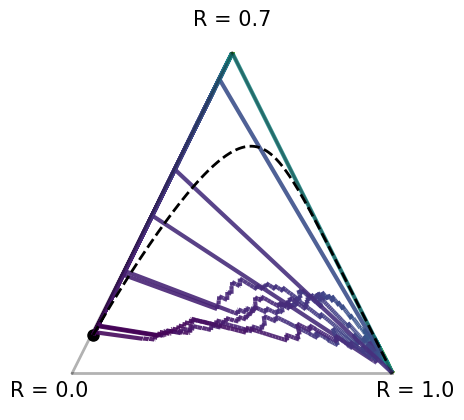
\includegraphics[width=\textwidth]{articles/baselines/figs/reproduced_simplex_npg/natural_minvar_-05.png}
    \caption{$b^-_\theta = b^*_\theta - \nicefrac{1}{2} $}
    \label{fig:-1}
  \end{subfigure}
  \hfill
    \begin{subfigure}[b]{0.24\linewidth}
    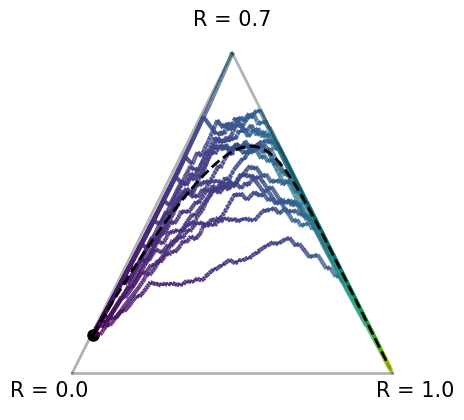
\includegraphics[width=\textwidth]{articles/baselines/figs/reproduced_simplex_npg/natural_minvar_00.png}
    \caption{$b_\theta = b^*_\theta$}
    \label{fig:0}
  \end{subfigure}
  \hfill
  \begin{subfigure}[b]{0.24\linewidth}
    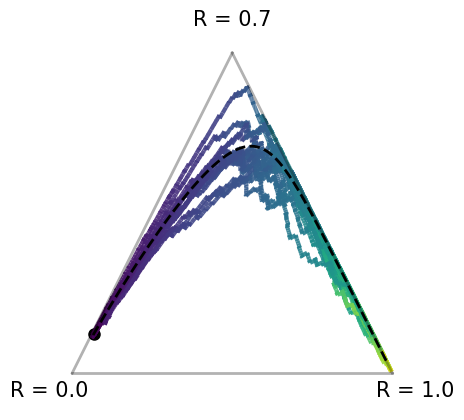
\includegraphics[width=\textwidth]{articles/baselines/figs/reproduced_simplex_npg/natural_minvar_05.png}
    \caption{$b^+_\theta = b^*_\theta + \nicefrac{1}{2}$}
    \label{fig:1}
  \end{subfigure}
  \hfill
  \begin{subfigure}[b]{0.24\linewidth}
    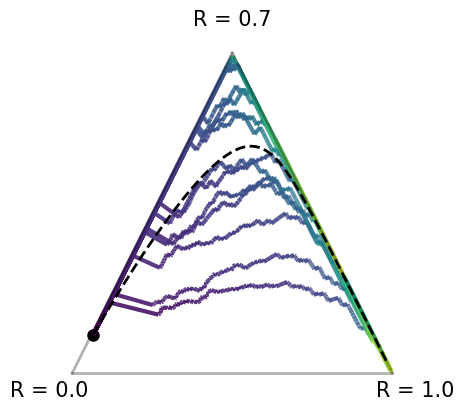
\includegraphics[width=\textwidth]{articles/baselines/figs/reproduced_simplex_npg/natural_value_00.png}
    \caption{$b_\theta=V^{\pi_\theta}$}
    \label{fig:v}
  \end{subfigure}
  \caption{ \label{fig:trajectories}  We plot 15 different trajectories of natural policy gradient with softmax parameterization, when using various baselines, on a 3-arm bandit problem with rewards $(1,0.7,0)$ and stepsize $\alpha = 0.025$ and $\theta_0 = (0, 3, 5)$. The black dot is the initial policy and colors represent time, from purple to yellow. The dashed black line is the trajectory when following the true gradient (which is unaffected by the baseline). Different values of $\epsilon$ denote different perturbations to the minimum-variance baseline. We see some cases of convergence to a suboptimal policy for both $\epsilon = -\nicefrac{1}{2}$ and $\epsilon = 0$. This does not happen for the larger baseline $\epsilon = \nicefrac{1}{2}$ or the value function as baseline. Figure made with Ternary~\citep{pythonternary}.}
\end{figure*}



\section{Baselines, learning dynamics \& exploration}
\label{sec:committal}

The problem defined in Eq.~\ref{eq:bandit_loss} can be solved by gradient ascent. Given access only to samples, the true gradient cannot generally be computed and the true update is replaced with a stochastic one, resulting in the following update:
\begin{align}
    \theta_{t+1} &= \theta_t + \frac{\alpha}{N} \sum_i r(a_i) \nabla_\theta \log \pi_\theta(a_i) \label{eq:mc_update} \; ,
\end{align}
where $a_i$ are actions drawn according to the agent's current policy $\pi_\theta$, $\alpha$ is the stepsize, and $N$, which can be 1, is the number of samples used to compute the update.
To reduce the variance of this estimate without introducing bias, we can introduce a baseline $b$, resulting in the gradient estimate $(r(a_i) - b) \nabla_\theta \log \pi_\theta(a_i)$.


While the choice of baseline is known to affect the variance, we show that baselines can also lead to qualitatively different behaviour of the optimization process, even when the variance is the same. This difference cannot be explained by the expectation or variance, quantities which govern the usual bounds for convergence rates~\citep{bottou2018optimization}. 


\subsection{Committal and non-committal behaviours}

To provide a complete picture of the optimization process, we analyze the evolution of the policy during optimization.
We start in a simple setting, a deterministic three-armed bandit, where it is easier to produce informative visualizations. 

To eliminate variance as a potential confounding factor, we consider different baselines with the same variance. We start by computing the baseline leading to the minimum-variance of the gradients for the algorithm we use. For vanilla policy gradient, we have $b^*_\theta = \frac{\E[r(a_i) \|\nabla \log \pi_\theta (a_i)\|^2_2 ] }{\E[ \|\nabla \log \pi_\theta (a_i) \|^2_2] } $ ~\citep{peters2008reinforcement, greensmith2004variance} (see Appendix~\ref{app:optimal_baseline} for details and the NPG version). Note that this baseline depends on the current policy and changes throughout the optimization. As the variance is a quadratic function of the baseline, the two baselines $b^+_\theta = b^*_\theta + \epsilon$ and $b^-_\theta = b^*_\theta - \epsilon$ result in gradients with the same variance (see Appendix \ref{app:var_perturbed_baseline} for details). Thus, we use these two perturbed baselines to demonstrate that there are phenomena in the optimization process that variance~cannot~explain.

Fig.~\ref{fig:trajectories} presents fifteen learning curves on the probability simplex representing the space of possible policies for the three-arm bandit, when using NPG and a softmax parameterization. We choose $\epsilon = \nicefrac{1}{2}$ to obtain two baselines with the same variance: $b^+_\theta = b^*_\theta + \nicefrac{1}{2}$ and $b^-_\theta = b^*_\theta - \nicefrac{1}{2}$.

Inspecting the plots, the learning curves for $\epsilon = -\nicefrac{1}{2}$ and $\epsilon = \nicefrac{1}{2}$ are qualitatively different, even though the gradient estimates have the same variance. For $\epsilon = -\nicefrac{1}{2}$, the policies quickly reach a deterministic policy (i.e., a neighborhood of a corner of the probability simplex), which can be suboptimal, as indicated by the curves ending up at the policy choosing action 2. On the other hand, for $\epsilon=\nicefrac{1}{2}$, every learning curve ends up at the optimal policy, although the convergence might be slower. The learning curves also do not deviate much from the curve for the true gradient. 
Again, these differences cannot be explained by the variance since the baselines result in identical variances. 


Additionally, for $b_\theta=b^*_\theta$, the learning curves spread out further. Compared to $\epsilon=\nicefrac{1}{2}$, some get closer to the top corner of the simplex, leading to convergence to a suboptimal solution, suggesting that the minimum-variance baseline may be worse than other, larger baselines. In the next section, we theoretically substantiate this and show that, for NPG, it is possible to converge to a suboptimal policy with the minimum-variance baseline; but there are larger baselines that guarantee convergence to an optimal~policy.

We look at the update rules to explain these different behaviours. When using a baseline $b$ with NPG, sampling $a_i$ results in the update
\begin{align*}
    \theta_{t+1} &= \theta_t + \alpha  [r(a_i)-b] F_\theta^{-1} \nabla_\theta \log \pi_\theta(a_i) \label{eq:npg_bandit_update} \\
    &= \theta_t + \alpha \frac{r(a_i)-b}{\pi_\theta(a_i)} \mathbf{1}_{a_i} + \alpha\lambda e
\end{align*}
where $F_\theta^{-1} = \E_{a \sim \pi} [\nabla \log \pi_\theta (a) \nabla \log \pi_\theta (a)^\top]$, $\mathbf{1}_{a_i}$ is a one-hot vector with $1$ at index $i$, and $\lambda e$ is a vector containing $\lambda$ in each entry.  The second line follows for the softmax policy (see Appendix \ref{app:npg_softmax_bandit}) and $\lambda$ is arbitrary since shifting $\theta$ by a constant does not change the policy.


Thus, supposing we sample action $a_i$, if $r(a_i) - b$ is positive, which happens more often when the baseline $b$ is small (more negative), the update rule will increase the probability $\pi_\theta(a_i)$. This leads to an increase in the probability of taking the actions the agent took before, regardless of their quality (see Fig.\ref{fig:-1} for $\epsilon=-\nicefrac{1}{2}$). Because the agent is likely to choose the same actions again, we call this \textit{committal} behaviour.

While a smaller baseline leads to committal behaviour, a larger (more positive) baseline makes the agent second-guess itself. If $r(a_i) - b$ is negative, which happens more often when $b$ is large, the parameter update decreases the probability $\pi_\theta(a_i)$ of the sampled action $a_i$, reducing the probability the agent will re-take the actions it just took, while increasing the probability of other actions. This might slow down convergence but it also makes it harder for the agent to get stuck. This is reflected in the $\epsilon = \nicefrac{1}{2}$ case (Fig.\ref{fig:1}), as all the learning curves end up at the optimal policy. We call this \textit{non-committal} behaviour.

While the previous experiments used perturbed variants of the minimum-variance baseline to control for the variance, this baseline would usually be infeasible to compute in more complex MDPs. Instead, a more typical choice of baseline would be the value function~\citep[Ch.~13]{sutton18book}, which we evaluate in Fig. \ref{fig:v}.
Choosing the value function as a baseline generated trajectories converging to the optimal policy, even though their convergence may be slow, despite it not being the minimum variance baseline.
The reason becomes clearer when we write the value function as $\displaystyle V^\pi = b^\ast_\theta - \tfrac{\textrm{Cov}(r, \|\nabla \log \pi\|^2)}{\E[\|\nabla \log \pi\|^2]}$ (see Appendix \ref{app:value_minvar_baseline}). The term $\textrm{Cov}(r, \|\nabla \log \pi\|^2)$ typically becomes negative as the gradient becomes smaller on actions with high rewards during the optimization process, leading to the value function being a noncommittal baseline, justifying a choice often made by practitioners. 

Additional empirical results can be found in Appendix \ref{app:exp_3armbandit} for natural policy gradient and vanilla policy gradient for the softmax parameterization. Furthermore, we explore the use of different parameterizations: First, we test projected stochastic gradient ascent and directly optimizing the policy probabilities $\pi_\theta(a)$. Next, we try the escort transform \citep{mei2020escaping}, which was designed to improve the curvature of the objective. We find qualitatively similar results in all cases; baselines can induce \textit{committal} and \textit{non-committal} behaviour. 

\section{Convergence to suboptimal policies with natural policy gradient (NPG)}

We empirically showed that PG algorithms can reach suboptimal policies and that the choice of baseline can affect the likelihood of this occurring. 
In this section, we provide theoretical results proving that it is indeed possible to converge to a suboptimal policy when using NPG. 
We discuss how this finding fits with existing convergence results and why standard assumptions are not satisfied in this setting. 

\subsection{A simple example}\label{sec:divergence_example}

Standard convergence results assume access to the true gradient~\citep[e.g.,][]{agarwal2019optimality} or, in the stochastic case, assume that the variance of the updates is uniformly bounded for all parameter values~\citep[e.g.,][]{bottou2018optimization}.
These assumptions are in fact quite strong and are violated in a simple two-arm bandit problem with fixed rewards. 
Pulling the optimal arm gives a reward of $r_1 = +1$, while pulling the suboptimal arm leads to a reward of $r_0 = 0$. We use the sigmoid parameterization and call $p_t = \sigma(\theta_t)$ the probability of sampling the optimal arm at time $t$.

Our stochastic estimator of the natural gradient is %
\begin{align*}
g_t = \left\{
                \begin{array}{l}
                  \frac{1 - b}{p_t}, \text{with probability}\ p_t \\
                  \frac{b}{1-p_t}, \text{with probability}\ 1-p_t,
                \end{array}
              \right.
\end{align*}
where $b$ is a baseline that does not depend on the action sampled at time $t$ but may depend on $\theta_t$. 
By computing the variance of the updates, $\textrm{Var}[g_t] =   \tfrac{(1-p_t - b)^2}{p_t (1-p_t)}$, we notice it is unbounded when the policy becomes deterministic, i.e. $p_t \to 0$ or $p_t \to 1$, violating the assumption of uniformly bounded variance, unless $b = 1-p_t$, which is the optimal baseline.
Note that using vanilla (non-natural) PG would, on the contrary, yield a bounded variance. In fact, we prove a convergence result in its favour in Appendix \ref{app:theory_2arm} (Prop. \ref{prop_vpg_cv}).

For NPG, the proposition below establishes potential convergence to a suboptimal arm and we demonstrate this~empirically~in~Fig.~\ref{fig:divergence_2arm_bandit}.

\begin{restatable}[]{proposition}{divtwoarms}
Consider a two-arm bandit with rewards $1$ and $0$ for the optimal and suboptimal arms, respectively. Suppose we use natural policy gradient starting from $\theta_0$, with a fixed baseline $b < 0$, and fixed stepsize $\alpha > 0$. If the policy samples the optimal action with probability $\sigma(\theta)$, then the probability of picking the suboptimal action forever and having $\theta_t$ go to $-\infty$ is strictly positive.
Additionally, if $\theta_0 \le 0$, we have
\[ P(\textup{suboptimal action forever}) \ge (1-e^{\theta_0}) (1-e^{\theta_0 + \alpha b})^{-\frac{1}{\alpha b}}. \]
\label{proposition_divergence}
\end{restatable}
\vspace{-0.8cm}
\begin{proof}
All the proofs may be found in the appendix.
\end{proof}

\begin{figure}[t!]
\centering
\begin{subfigure}[b]{0.32\linewidth}   
    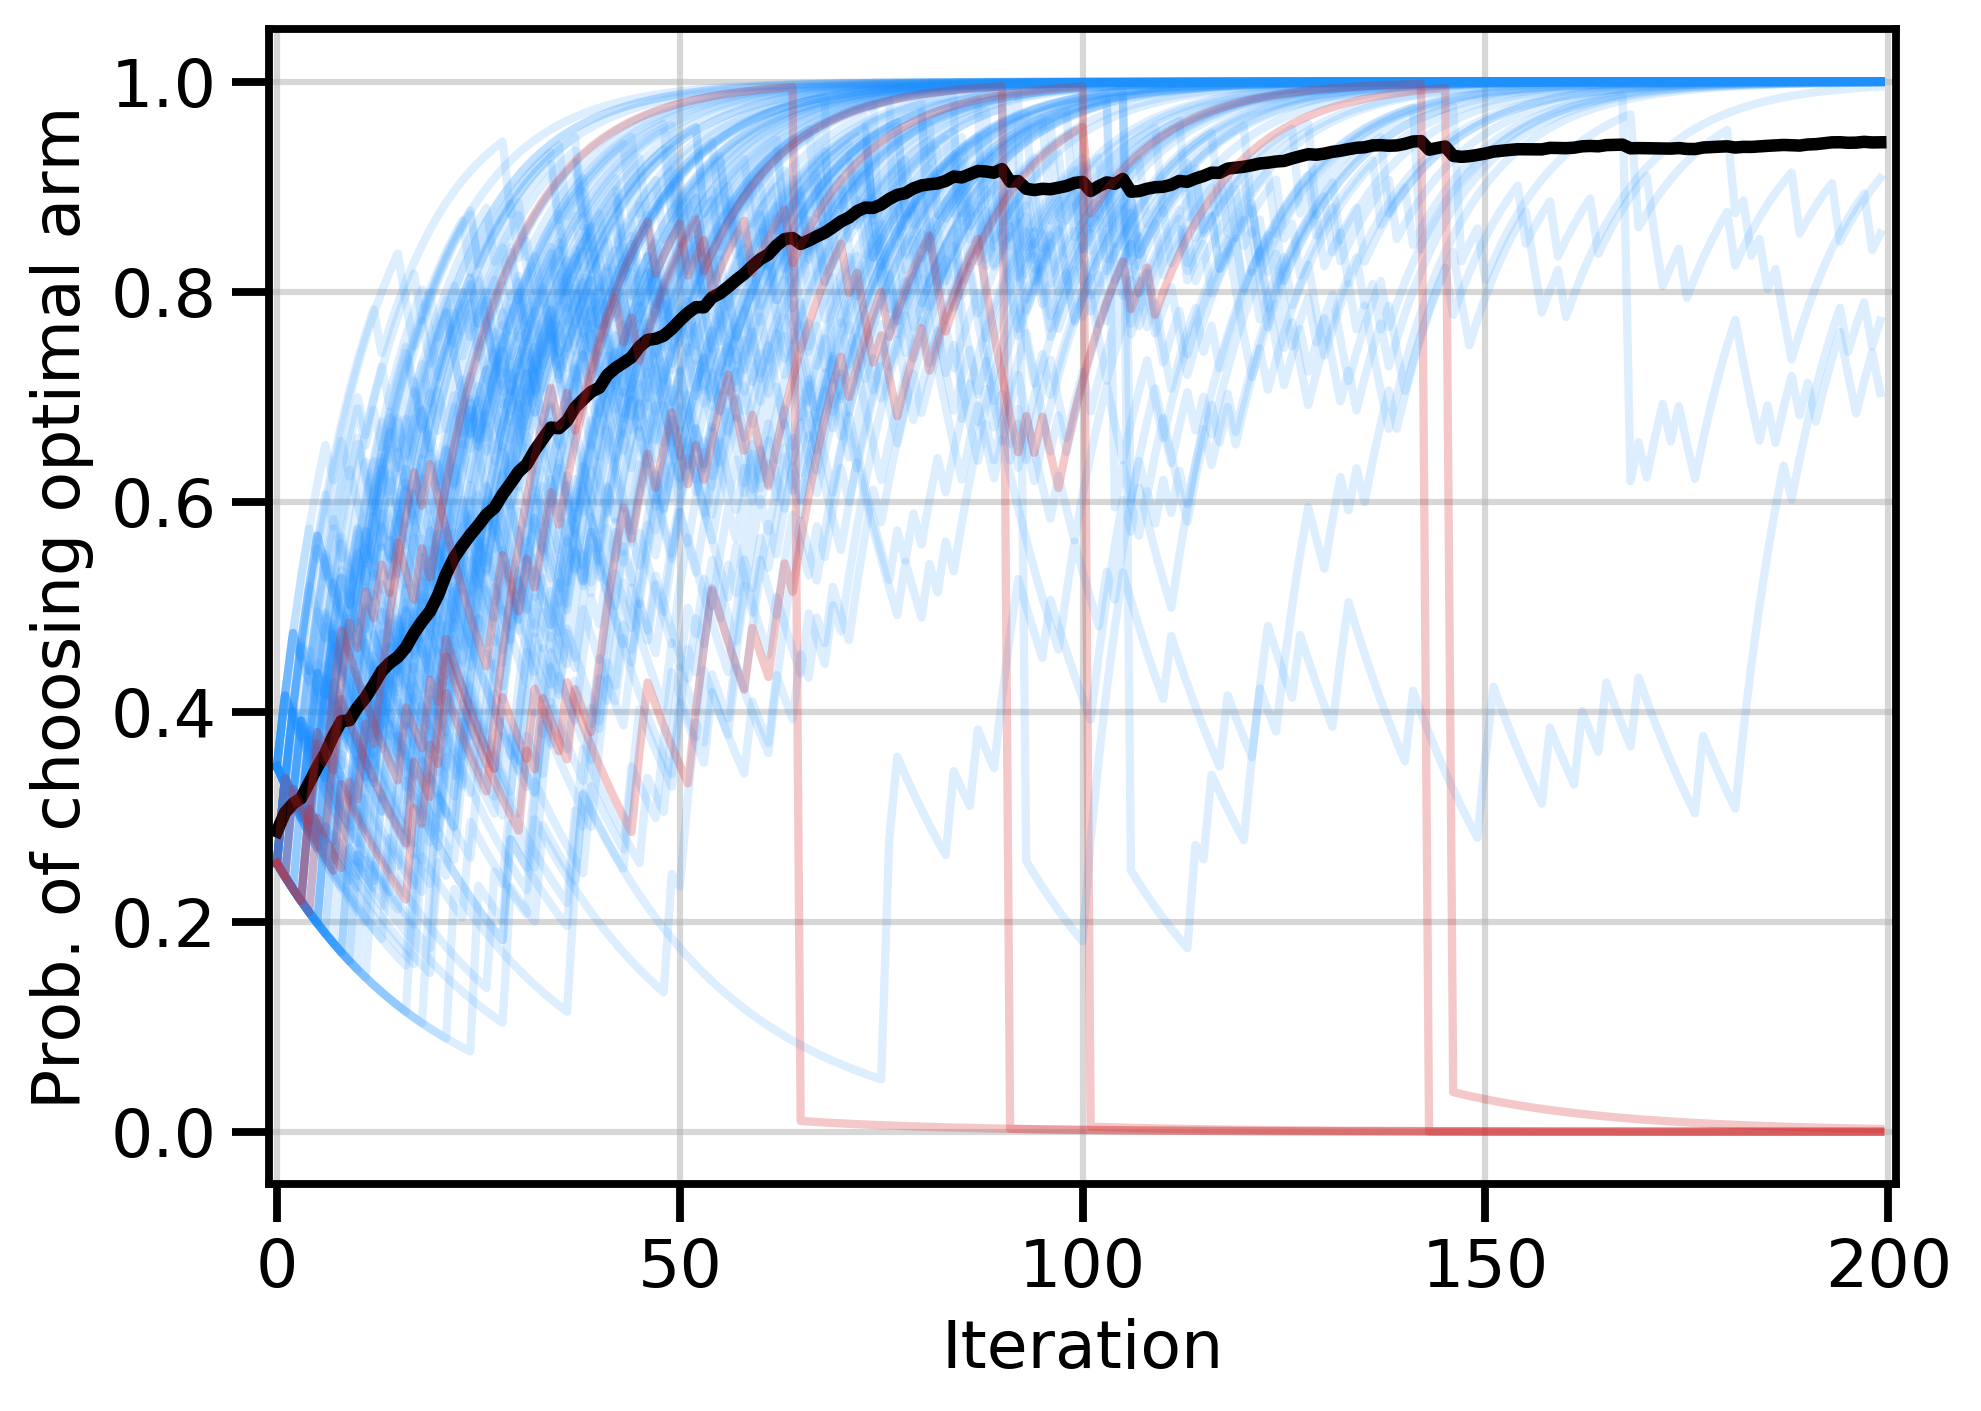
\includegraphics[width=\textwidth]{articles/baselines/figs/paper/bandit_committal_005.png}
    \caption{$\alpha=0.05$}
\end{subfigure}
\begin{subfigure}[b]{0.32\linewidth}   
    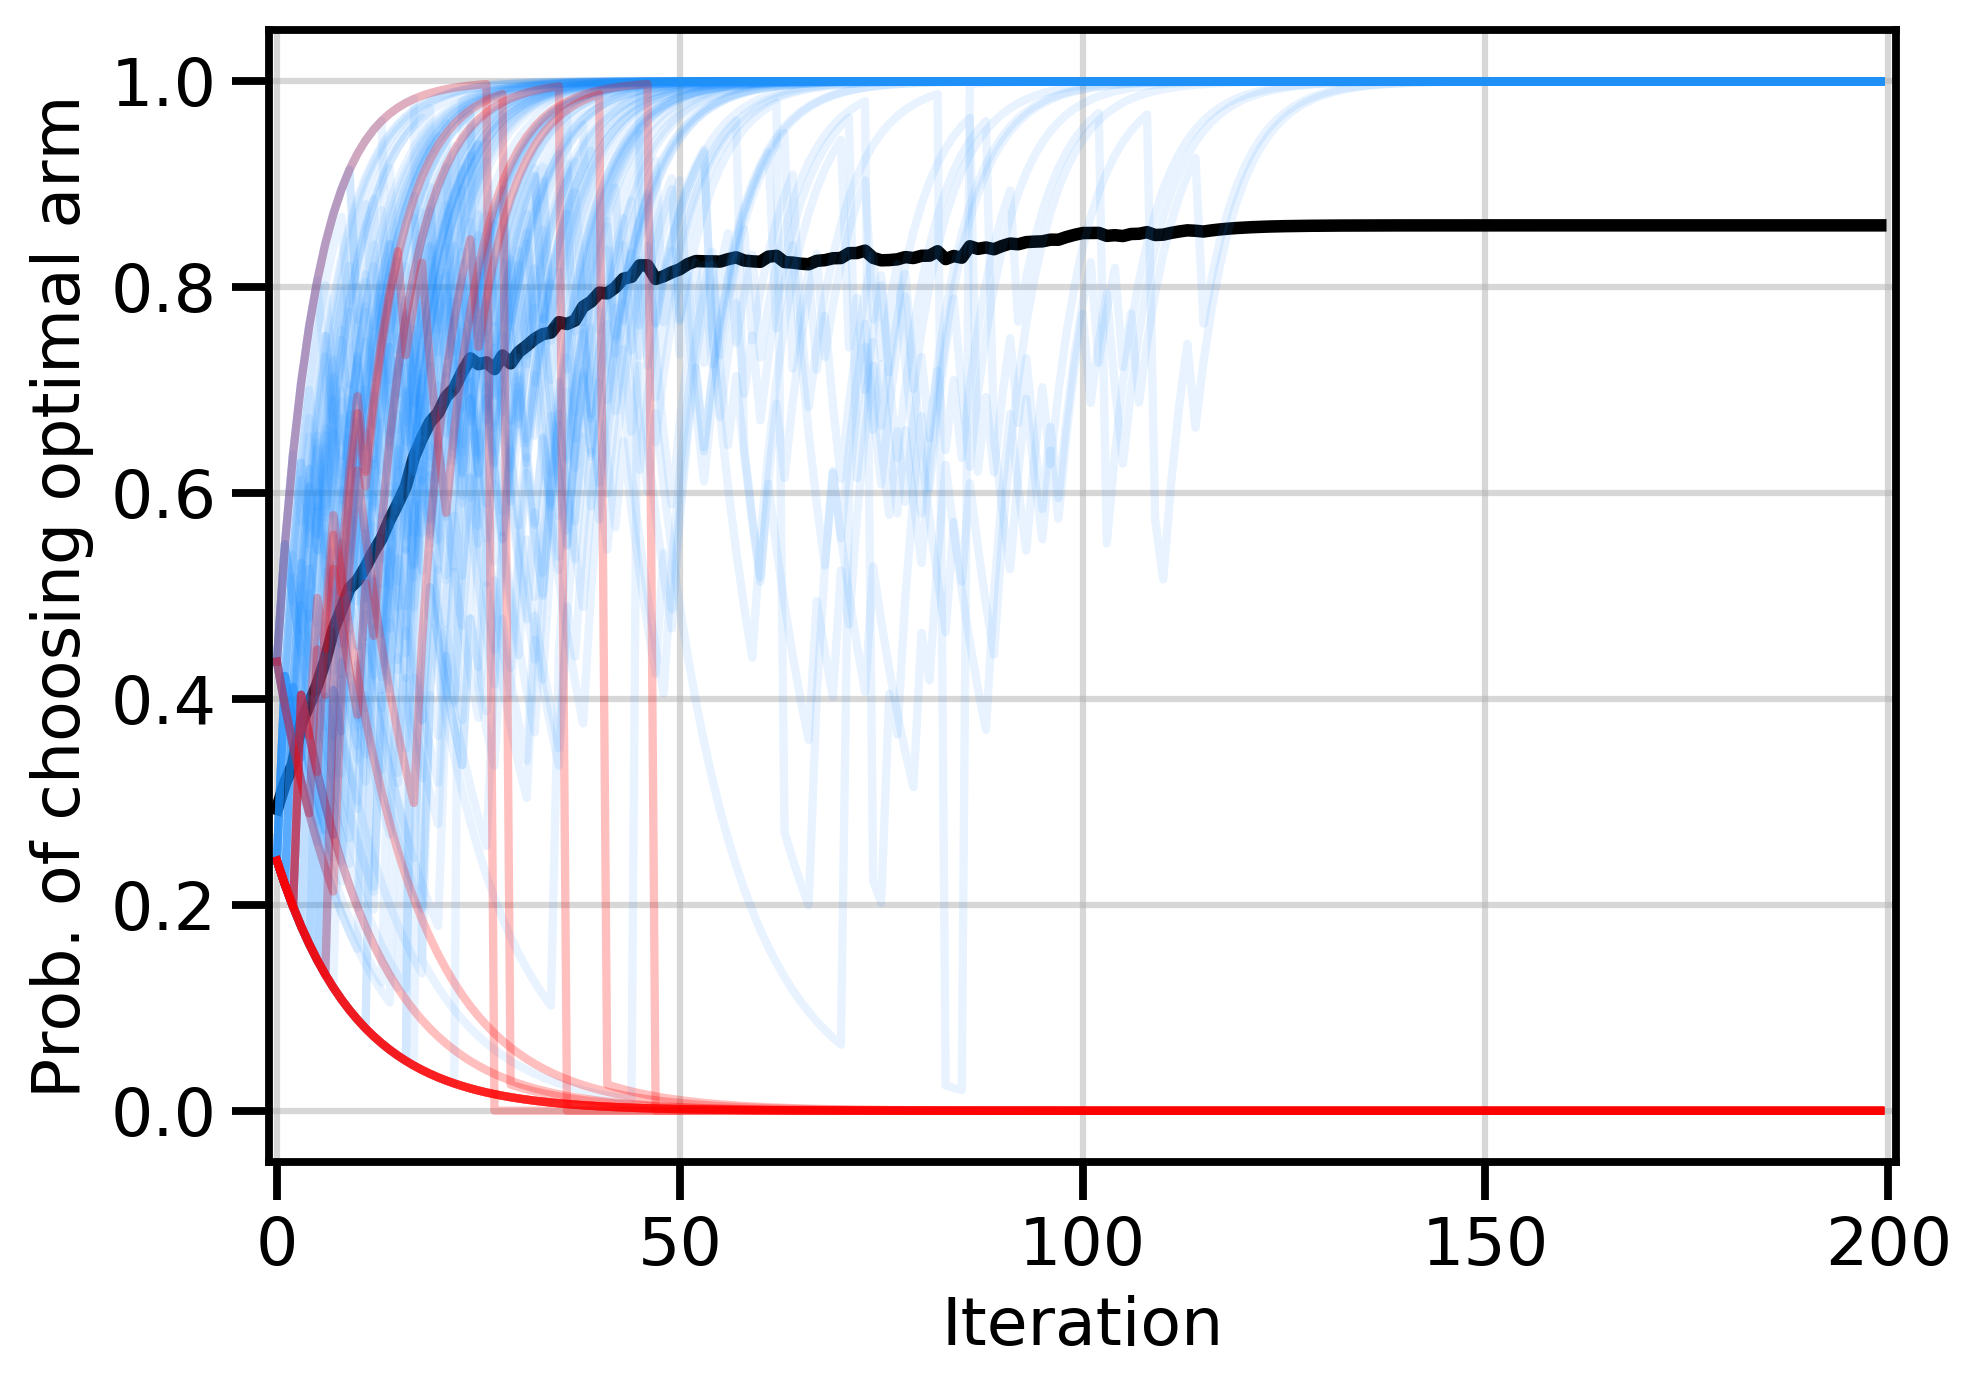
\includegraphics[width=\textwidth]{articles/baselines/figs/paper/bandit_committal.png}
    \caption{$\alpha=0.1$}
\end{subfigure}
\begin{subfigure}[b]{0.32\linewidth}   
    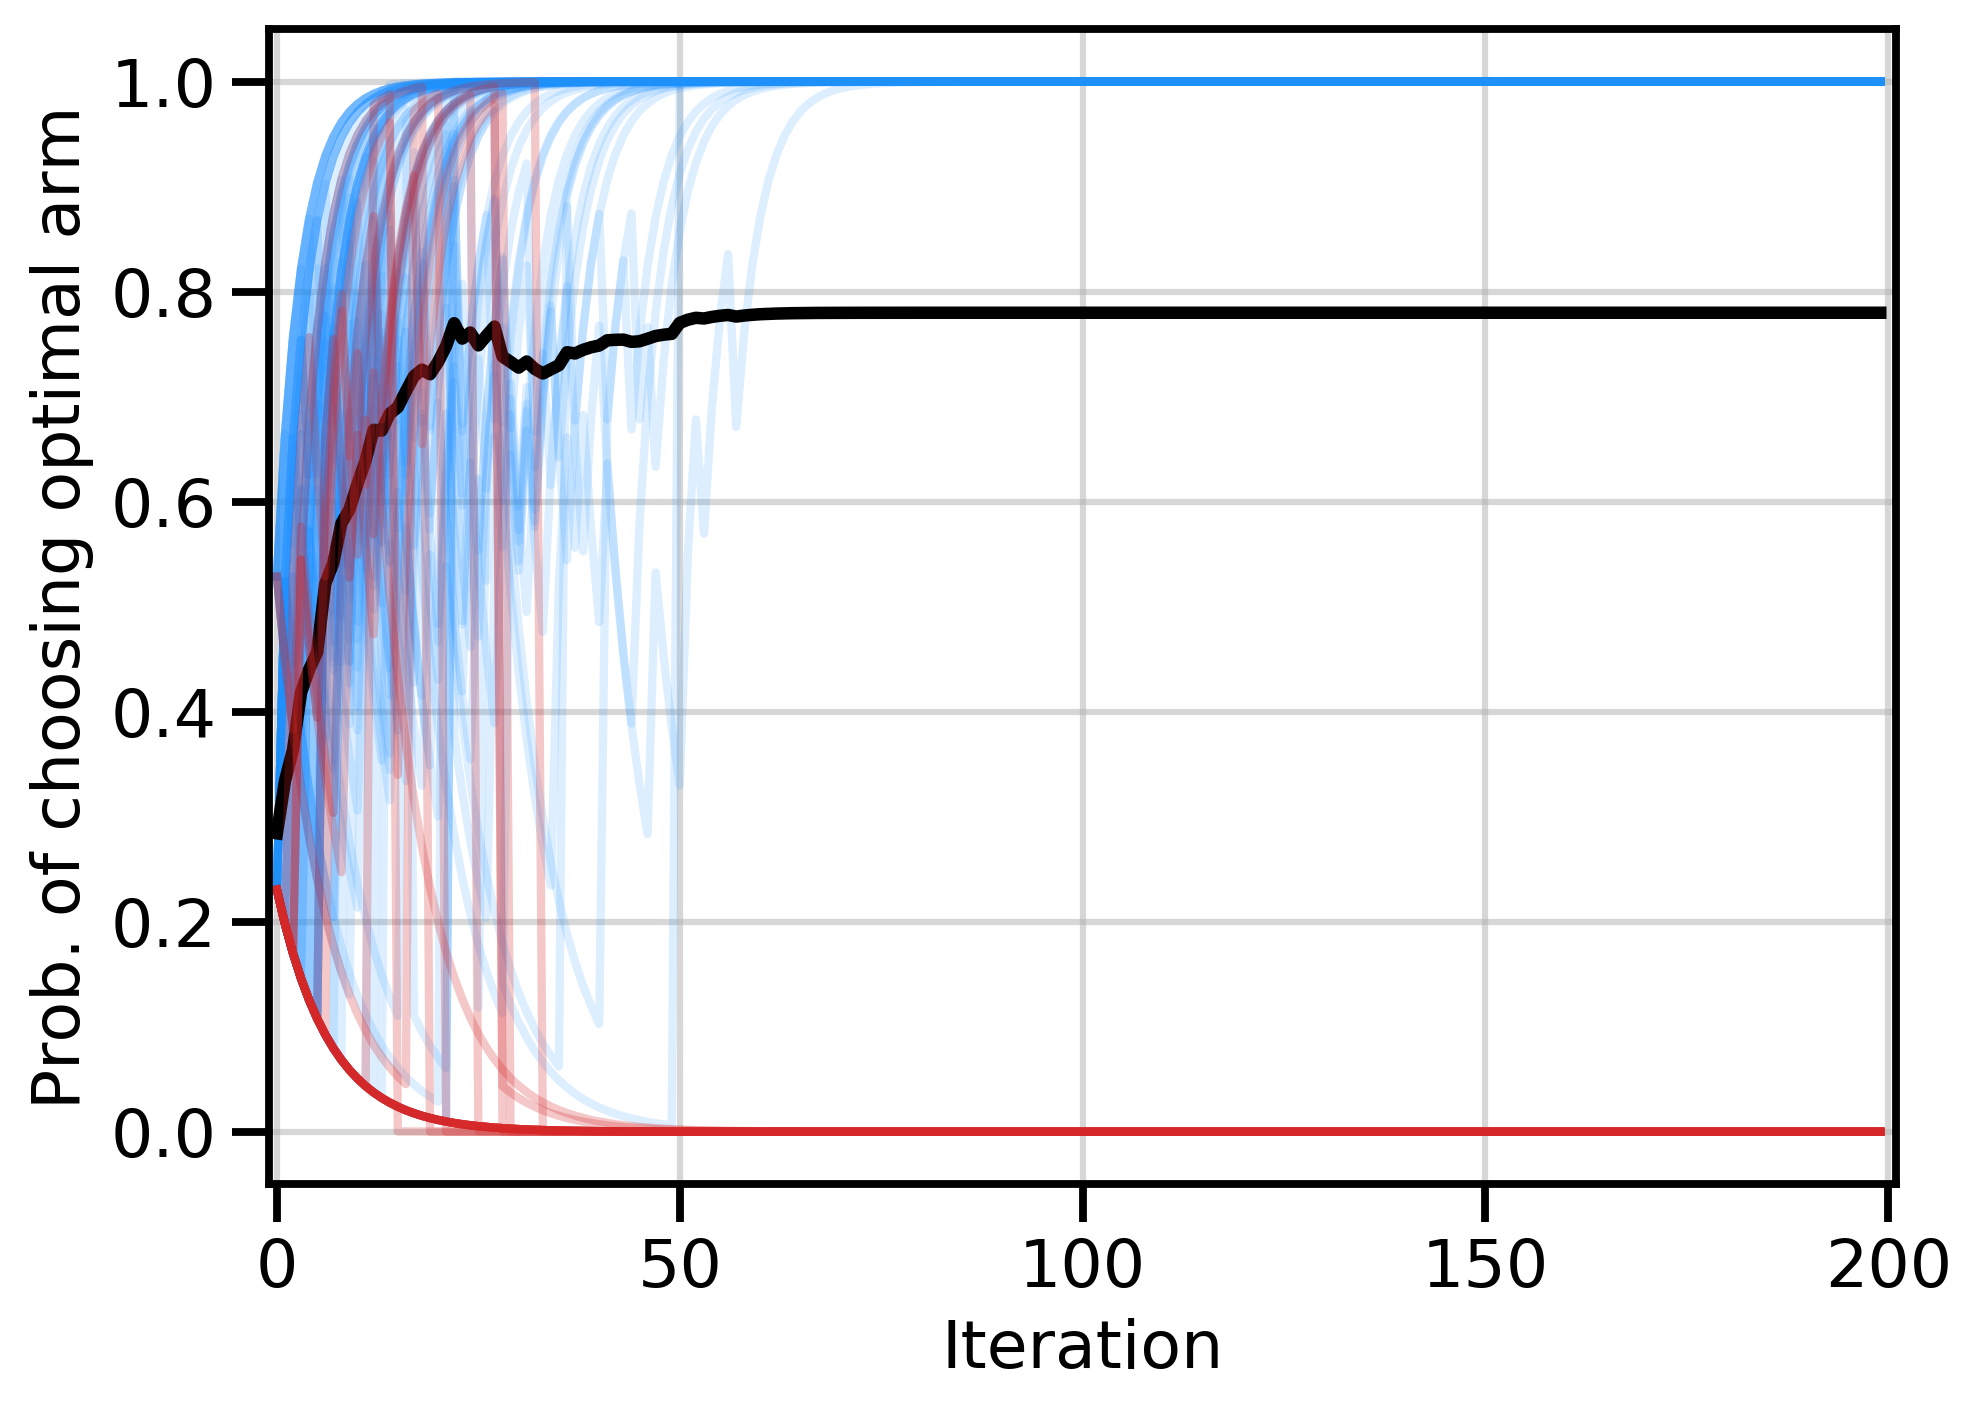
\includegraphics[width=\textwidth]{articles/baselines/figs/paper/bandit_committal_015.png}
    \caption{$\alpha=0.15$}
\end{subfigure}

\caption{Learning curves for 100 runs of 200 steps, on the two-arm bandit, with baseline $b\!=\!-1$ for three different stepsizes $\alpha$. \emph{Blue:} Curves converging to the optimal policy. \emph{Red:} Curves  converging to a suboptimal policy. \emph{Black:} Avg. performance. 
The number of runs that converged to the suboptimal solution are 5\%, 14\% and 22\% for the three $\alpha$'s. Larger $\alpha$'s are more prone to getting stuck at a suboptimal solution but settle on a deterministic policy more quickly.}
\label{fig:divergence_2arm_bandit}
\end{figure}

The updates provide some intuition as to why there is convergence to suboptimal policies. The issue is the \textit{committal} nature of the baseline. Choosing an action leads to an increase of that action's probability, even if it is a poor choice. Choosing the suboptimal arm leads to a decrease in $\theta$ by $\tfrac{\alpha b}{1-p_t}$, thus increasing the probability the same arm is drawn again and further decreasing $\theta$. By checking the probability of this occurring forever, $P(\text{suboptimal arm forever}) = \prod_{t=1}^\infty (1-p_t)$, we show that $1-p_t$ converges quickly enough to 1 that the infinite product is nonzero, showing it is possible to get trapped choosing the wrong arm forever~(Prop. \ref{proposition_divergence}), and $\theta_t \to -\infty$ as $t$ grows.

This issue could be solved by picking a baseline with lower variance. For instance, the minimum-variance baseline $b = 1 - p_t$ leads to $0$ variance and both possible updates are equal to $+\alpha$, guaranteeing that $\theta \to +\infty$, thus convergence. In fact, any baseline $b \in (0,1)$ suffices since both updates are positive and greater than $\alpha \min(b, 1-b)$. However, this is not always the case, as we show in the next section.

To decouple the impact of the variance with that of the committal nature of the baseline, Prop.~\ref{prop:2armed-perturbedminvar} analyzes the learning dynamics in the two-arm bandit case for perturbations of the optimal baseline, i.e. we study baselines of the form $b = b^* + \epsilon$ and show how $\epsilon$, and particularly its sign, affects learning. Note that, because the variance is a quadratic function with its minimum in $b^*$, both $+\epsilon$ and $-\epsilon$ have the same variance. Our findings can be summarized as follows:
\begin{proposition}
    \label{prop:2armed-perturbedminvar}
    For the two-armed bandit defined in Prop.~\ref{proposition_divergence}, when using a perturbed min-variance baseline $b = b^* + \epsilon$, the value of $\epsilon$ determines the learning dynamics as follows:
    \begin{itemize}%
        \item For $\epsilon < -1$, there is a positive probability of converging to the suboptimal arm.
        \item For $\epsilon \in (-1, 1)$, we have convergence in probability to the optimal policy.
        \item For $\epsilon \ge 1$, the supremum of the iterates goes to $+\infty$ in probability.
    \end{itemize}
\end{proposition}


While the proofs can be found in Appendix~\ref{sec:appendix_perturbed_minvar}, we provide here some intuition behind these results.

For $\epsilon < -1$, we reuse the same argument as for $b<0$ in Prop.~\ref{proposition_divergence}. The probability of drawing the correct arm can decrease quickly enough to lead to convergence to the suboptimal arm.

For $\epsilon \in (-1,1)$, the probability of drawing the correct arm cannot decrease too fast. Hence, although the updates, as well as the variance of the gradient estimate, are potentially unbounded, we still have convergence to the optimal solution in probability.

Finally, for $\eps \ge 1$, we can reuse an intermediate argument from the $\epsilon \in (0,1)$ case to argue that for any threshold $C$, the parameter will eventually exceed that threshold. For $\epsilon \in (0,1)$, once a certain threshold is crossed, the policy is guaranteed to improve at each step. However, with a large positive perturbation, updates are larger and we lose this additional guarantee, leading to the weaker result.

We want to emphasize that not only we get provably different dynamics for $\epsilon < -1$ and $\eps \ge 1$, showing the importance of the sign of the perturbation, but that there also is a sharp transition around $|\epsilon| = 1$, which cannot be captured solely by the variance.

The above analysis was specific to these updates. To predict committal vs. non-committal behaviour more generally, it may be possible to utilize higher order moments or other distributional properties, even when the mean and variance is the same.
Unfortunately, it is difficult to utilize higher-moment information in theoretical bounds in a general manner as Markov-type inequalities do not take into account the sign of the higher moment, which we think is where the committal vs. non-committal distinction would appear.




\subsection{Reducing variance with baselines can be detrimental}
\label{sec:reducing_detrimental}
As we saw with the two-armed bandit, the direction of the updates is important in assessing convergence. More specifically, problems can arise when the choice of baseline induces committal behaviour.
We now show a different bandit setting where committal behaviour happens even when using the minimum-variance baseline, thus leading to convergence to a suboptimal policy. Furthermore, we design a better baseline which ensures all updates move the parameters towards the optimal policy. This cements the idea that the quality of parameter updates must not be analyzed in terms of variance but rather in terms of the probability of going in a bad direction, since a baseline that induces higher variance leads to convergence while the minimum-variance baseline does not.
The following theorem summarizes this.

\begin{restatable}[]{theorem}{threearmedbandit}
There exists a three-arm bandit where using the stochastic natural gradient on a softmax-parameterized policy with the minimum-variance baseline can lead to convergence to a suboptimal policy with probability $\rho > 0$, and there is a different baseline (with larger variance) which results in convergence to the optimal policy with probability~1.
\label{proposition_threearmedbandit}
\end{restatable}
The bandit used in this theorem is the one we used for the experiments depicted in Fig.~\ref{fig:trajectories}.
The key is that the minimum-variance baseline can be lower than the second best reward; so pulling the second arm will increase its probability and induce committal behaviour.
This can cause the agent to prematurely commit to the second arm and converge to the wrong policy.
On the other hand, using any baseline whose value is between the optimal reward and the second best reward, which we term a \textit{gap} baseline, will always increase the probability of the optimal action at every step, no matter which arm is drawn. Since the updates are sufficiently large at every step, this is enough to ensure convergence with probability 1, despite the higher variance compared to the minimum variance baseline.
The key is that whether a baseline underestimates or overestimates the second best reward can affect the algorithm convergence and this is more critical than the resulting variance of the gradient estimates.


As such, more than lower variance, good baselines are those that can assign positive effective returns to the good trajectories and negative effective returns to the others. These results cast doubt on whether finding baselines which minimize variance is a meaningful goal to pursue. The baseline can affect optimization in subtle ways, beyond variance, and further study is needed to identify the true causes of some improved empirical results observed in previous works. This importance of the sign of the returns, rather than their exact value, echoes with the cross-entropy method~\citep{de2005tutorial}, which maximizes the probability of the trajectories with the largest returns, regardless of their actual value.


\section{Off-policy sampling} 

So far, we have seen that \textit{committal} behaviour can be problematic as it can cause convergence to a suboptimal policy. This can be especially problematic when the agent follows a near-deterministic policy as it is unlikely to receive different samples which would move the policy away from the closest deterministic one, regardless of the quality of that policy.

Up to this point, we assumed that actions were sampled according to the current policy, a setting known as \emph{on-policy}. This setting couples the updates and the policy and is a root cause of the \textit{committal} behaviour: the update at the current step changes the policy, which affects the distribution of rewards obtained and hence the next updates. 
However, we know from the optimization literature that bounding the variance of the updates will lead to convergence \citep{bottou2018optimization}. As the variance becomes unbounded when the probability of drawing some actions goes to 0, a natural solution to avoid these issues is to sample actions from a behaviour policy that selects every action with sufficiently high probability.
Such a policy would make it impossible to choose the same, suboptimal action forever. 

\subsection{Convergence guarantees with IS}

Because the behaviour policy changed, we introduce importance sampling (IS) corrections to preserve the unbiased updates~\citep{kahn1951estimation, precup2000eligibility}. 
These changes are sufficient to guarantee convergence for any baseline:

\begin{restatable}[]{proposition}{is}
\label{lem:main_off-policy_IS}
Consider a $n$-armed bandit with stochastic rewards with bounded support and a unique optimal action. The behaviour policy $\mu_t$ selects action $i$ with probability $\mu_t(i)$ and let $\epsilon_t = \min_i \mu_t(i)$. When using NPG with importance sampling and a bounded baseline $b$, if $\lim_{t \to \infty} t \ \epsilon_t^2 = +\infty$ , then the target policy $\pi_t$ converges to the optimal policy in probability.
\end{restatable}
\begin{proof} 
\textit{(Sketch)}
Using Azuma-Hoeffding's inequality, we can show that for well chosen constants $\Delta_i, \delta$ and $C > 0$ ,
\begin{eqnarray*}
\sP\left( \theta_t^1 \ge  \theta_0^1 + \alpha \delta \Delta_1 t\right) %
&\ge& 1- \exp \left( -\frac{\delta^2 \Delta_1^2}{2 C^2}t \epsilon_t^2 \right)\\
\end{eqnarray*} 
where $\theta^1$ is the parameter associated to the optimal arm.
Thus if $\lim_{t\to\infty} t \epsilon_t^2 = +\infty$, the RHS goes to $1$. 
In a similar manner, we can upper bound $\sP\left( \theta_t^i \ge  \theta_0^i + \alpha \delta \Delta_i t\right)$ for all suboptimal arms, and 
applying an union bound, we get the desired result.
\end{proof}
\vspace{-3mm}

The condition on $\mu_t$ imposes a cap on how fast the behaviour policy can become deterministic: no faster than $t^{-1/2}$. Intuitively, this ensures each action is sampled sufficiently often and prevents premature convergence to a suboptimal policy.
The condition is satisfied for any sequence of behaviour policies which assign at least $\epsilon_t$ probability to each action at each step, such as $\epsilon$-greedy policies. It also holds if $\epsilon_t$ decreases over time at a sufficiently slow rate. By choosing as behaviour policy $\mu$ a linear interpolation between $\pi$ and the uniform policy, $\mu(a) = (1-\gamma) \pi(a) + \frac{\gamma}{K}, \gamma \in (0,1]$, where $K$ is the number of arms, we recover the classic EXP3 algorithm~\citep{auer2002nonstochastic, seldin2012evaluation}.

We can also confirm that this condition is not satisfied for the simple example we presented when discussing convergence to suboptimal policies. There, $p_t$ could decrease exponentially fast since the tails of the sigmoid function decay exponentially and the parameters move by at least a constant at every step. In this case, $\epsilon_t = \Omega (e^{-t})$, resulting in $\lim_{t\to \infty} t e^{-2 t} = 0$, so Proposition~\ref{lem:main_off-policy_IS} does not apply.

\subsection{Importance sampling, baselines \& variance}
As we have seen, using a separate behaviour policy that samples all actions sufficiently often may lead to stronger convergence guarantees, even if it increases the variance of the gradient estimates in most of the space, as what matters is what happens in the high variance regions, which are usually close to the boundaries. Fig.~\ref{fig:simplex_variance} shows the ratios of gradient variances between on-policy PG without baseline, on-policy PG with the minimum variance baseline, and off-policy PG using importance sampling~(IS) where the sampling distribution is $\mu(a) = \frac{1}{2} \pi(a) + \frac{1}{6}$, i.e. a mixture of the current policy $\pi$ and the uniform distribution. While using the minimum variance baseline decreases the variance on the entire space compared to not using a baseline, IS actually \emph{increases} the variance when the current policy is close to uniform. However, IS does a much better job at reducing the variance close to the boundaries of the simplex, where it actually matters to guarantee convergence.

\begin{figure}[t!]
\begin{center}
    \begin{subfigure}[b]{0.08\linewidth}
    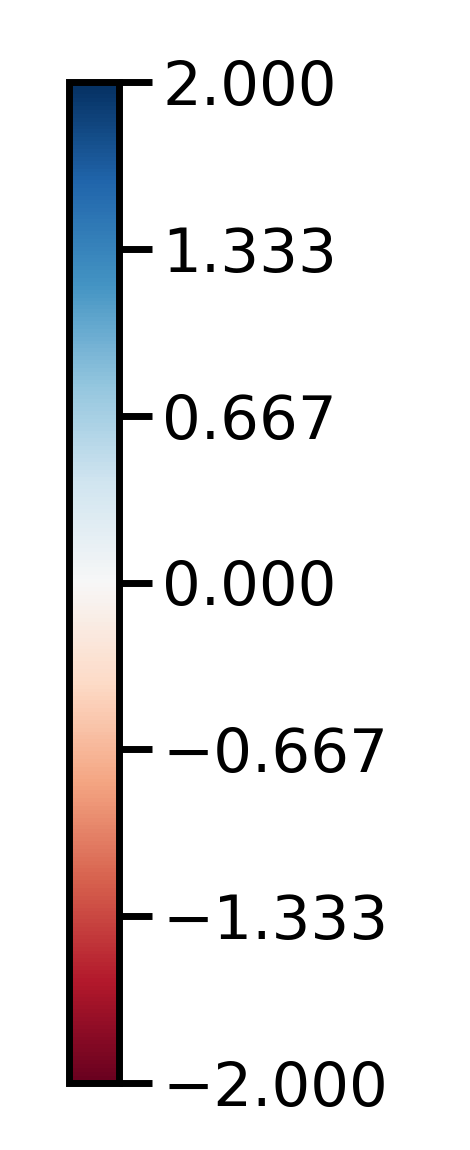
\includegraphics[trim={2cm 1.5cm 2cm 0},clip,width=\textwidth]{articles/baselines/figs/simplex_plots/colorbar_vertical.png}
    \label{fig:is_baseline}
  \end{subfigure}
  \begin{subfigure}[b]{.27\linewidth}
    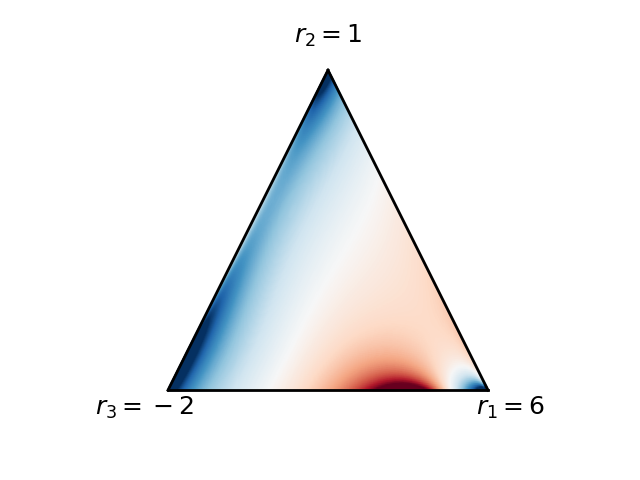
\includegraphics[trim={2cm 1.5cm 2cm 0mm},clip, width=\textwidth]{articles/baselines/figs/simplex_plots/v_vs_is.png}
    \caption{{\color{myred}$b=0$} / {\color{myblue}IS}.}
  \end{subfigure}
  \begin{subfigure}[b]{0.27\linewidth}
    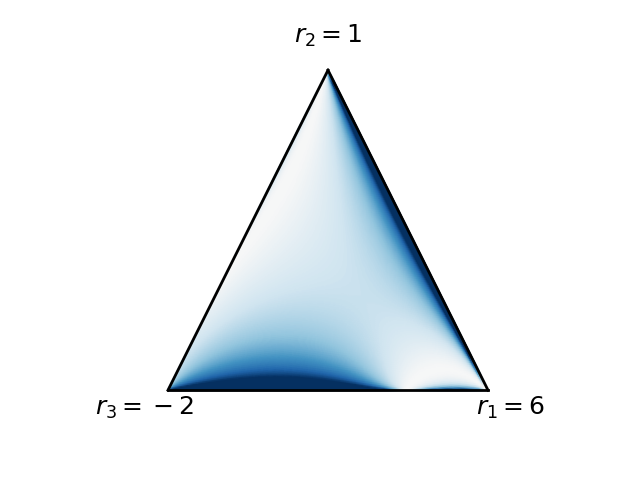
\includegraphics[trim={2cm 1.5cm 2cm 0},clip,width=\textwidth]{articles/baselines/figs/simplex_plots/v_vs_b.png}
    \caption{{\color{myred}$b=0$} / {\color{myblue}$b^\ast$}.}
  \end{subfigure}
  \begin{subfigure}[b]{0.27\linewidth}
    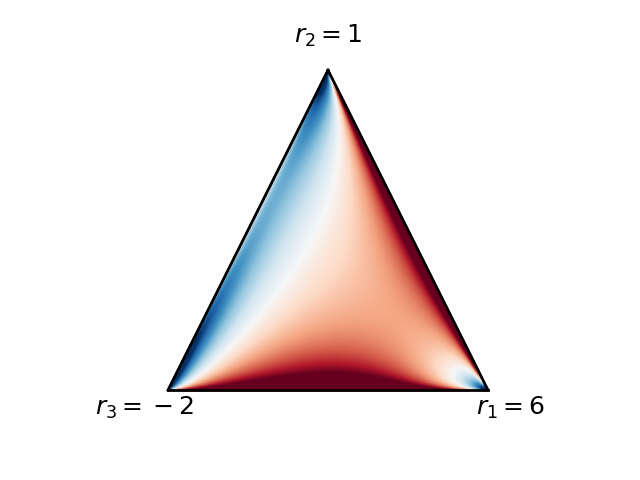
\includegraphics[trim={2cm 1.5cm 2cm 0},clip,width=\textwidth]{articles/baselines/figs/simplex_plots/b_vs_is.png}
    \caption{{\color{myred}$b^\ast$} / {\color{myblue}IS}.}
  \end{subfigure}
\caption{Comparison between the variance of different methods on a 3-arm bandit. Each plot depicts the $\log$ of the ratio between the variance of two approaches. For example, Fig. (a) depicts $\log \tfrac{\textrm{Var}[g_{b=0}]}{\textrm{Var}[g_{\text{IS}}]}$, the $\log$ of the ratio between the variance of the gradients of PG without a baseline and PG with IS. The triangle represents the probability simplex with each corner representing a deterministic policy on a specific arm. The method written in blue (resp. red) in each figure has lower variance in blue (resp. red) regions of the simplex. The sampling policy $\mu$, used in the PG method with IS, is a linear interpolation between $\pi$ and the uniform distribution, $\mu(a) = \frac{1}{2} \pi(a) + \frac{1}{6}$. Note that this is not the min. variance sampling distribution and it leads to higher variance than PG without a baseline in some parts of the simplex.} \label{fig:simplex_variance}
\end{center}
\end{figure}

This suggests that convergence of PG methods is not so much governed by the variance of the gradient estimates in general, but by the variance in the worst regions, usually near the boundary. While baselines can reduce the variance, they generally cannot prevent the variance in those regions from exploding, leading to the policy getting stuck. Thus, good baselines are not the ones reducing the variance across the space but rather those that can prevent the learning from reaching these regions altogether. Large values of $b$, such that $r(a_i) - b$ is negative for most actions, achieve precisely that. On the other hand, due to the increased flexibility of sampling distributions, IS can limit the nefariousness of these critical regions, offering better convergence guarantees despite not reducing variance~everywhere.

Importantly, although IS is usually used in RL to correct for the distribution of past samples~\citep[e.g.,][]{munos16retrace}, we advocate here for expanding the research on designing appropriate sampling distributions as done by~\citet{hanna2017data, hanna2018importance} and \citet{parmas2019unified}. This line of work has a long history in statistics~\citep[c.f.,][]{liu2008monte}. 

\subsection{Other mitigating strategies}
We conclude this section by discussing alternative strategies to mitigate the convergence issues. While they might be effective, and some are indeed used in practice, they are not without pitfalls.

First, one could consider reducing the stepsizes, with the hope that the policy would not converge as quickly towards a suboptimal deterministic policy and would eventually leave that bad region. Indeed, if we are to use vanilla PG in the two-arm bandit example, instead of NPG, this effectively reduces the stepsize by a factor of $\sigma(\theta)(1-\sigma(\theta))$ (the Fisher information). In this case, we are able to show convergence in probability to the optimal policy. See Proposition~\ref{prop_vpg_cv} in Appendix \ref{app:theory_2arm}.

Empirically, we find that, when using vanilla PG, the policy may still remain stuck near a suboptimal policy when using a negative baseline, similar to Fig.~\ref{fig:divergence_2arm_bandit}. While the previous proposition guarantees convergence eventually, the rate may be very slow, which remains problematic in practice. There is theoretical evidence that following even the true vanilla PG may result in slow convergence~\citep{schaul2019ray}, suggesting that the problem is not necessarily due to noise.

An alternative solution would be to add entropy regularization to the objective. By doing so, the policy would be prevented from getting too close to deterministic policies. While this might prevent convergence to a suboptimal policy, it would also exclude the possibility of fully converging to the optimal policy, though the policy may remain near it.

In bandits, EXP3 has been found not to enjoy high-probability guarantees on its regret so variants have been developed to address this deficiency \citep[c.f.][]{lattimore_szepesvari_2020}. For example, by introducing bias in the updates, their variance can be reduced significantly \cite{auer2002nonstochastic, neu2015explore}.
Finally, other works have also developed provably convergent policy gradient algorithms using different mechanisms, such as exploration bonuses or ensembles of policies~\citep{cai2019provably, efroni2020optimistic, agarwal2020pc}. 


\section{Extension to multi-step MDPs}
\begin{figure*}
\centering
 \begin{subfigure}[b]{0.21\linewidth}   
    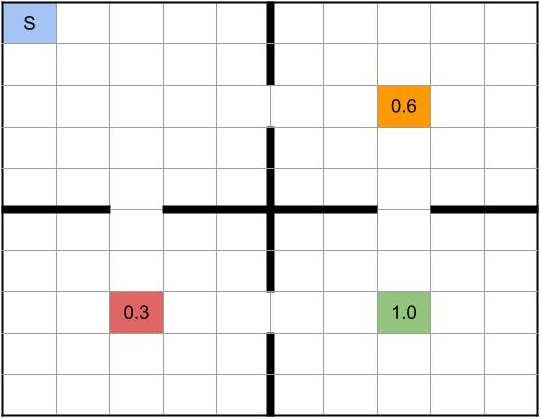
\includegraphics[trim={0cm -0.8cm 0cm 0},clip,width=\textwidth]{articles/baselines/figs/paper/Four_rooms.jpg}
    \caption{MDP}
    \label{fig:4rooms_mdp}
  \end{subfigure}
  \begin{subfigure}[b]{0.25\linewidth}
    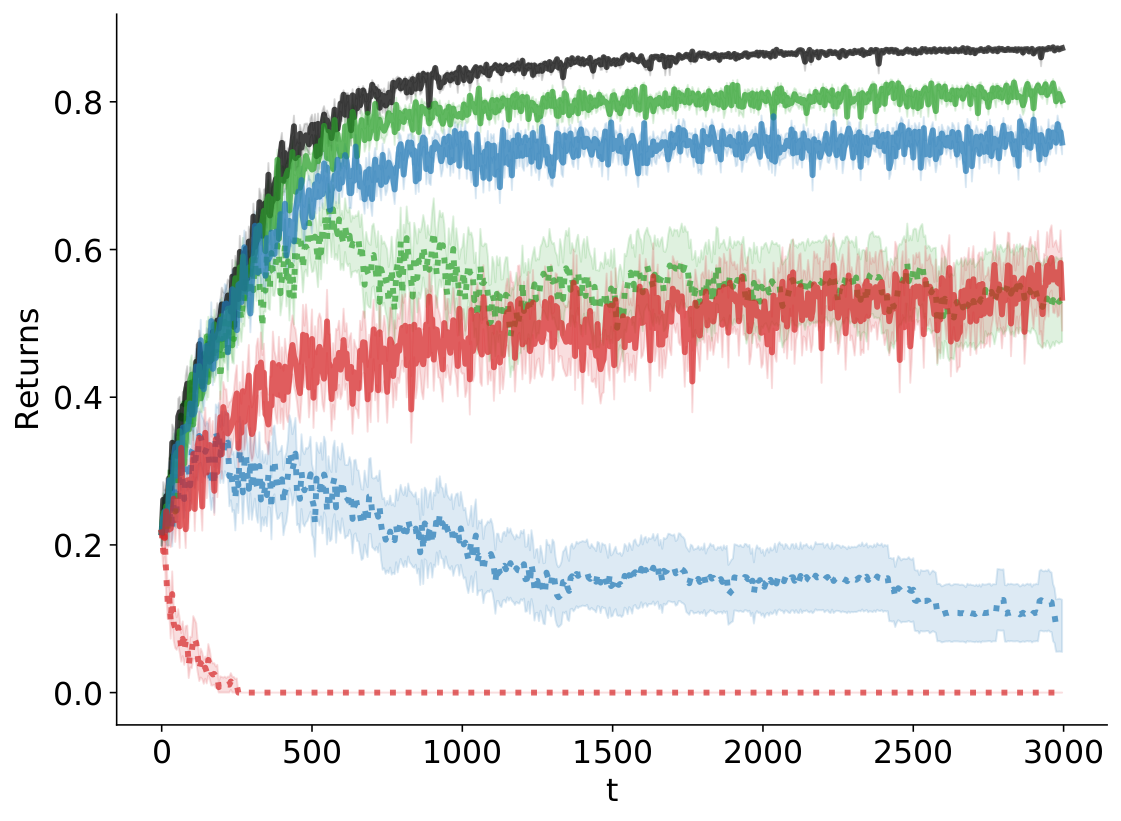
\includegraphics[width=\textwidth]{articles/baselines/figs/baseline_4rooms/NPG_returns.png}
    \caption{Returns}
    \label{fig:4rooms_return}
  \end{subfigure}
    \begin{subfigure}[b]{0.25\linewidth}
    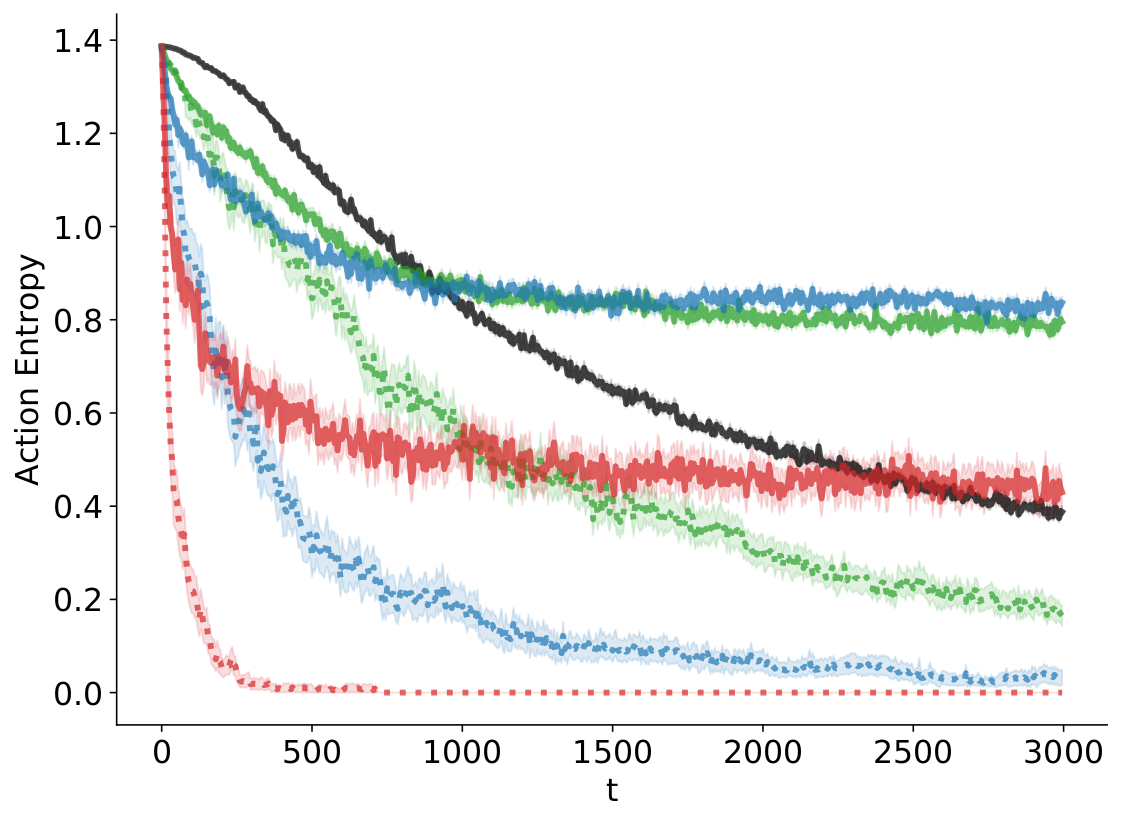
\includegraphics[width=\textwidth]{articles/baselines/figs/baseline_4rooms/NPG_action_entropy.png}
    \caption{Entropy (A)}
    \label{fig:4rooms_action}
  \end{subfigure}
  \begin{subfigure}[b]{0.25\linewidth}
    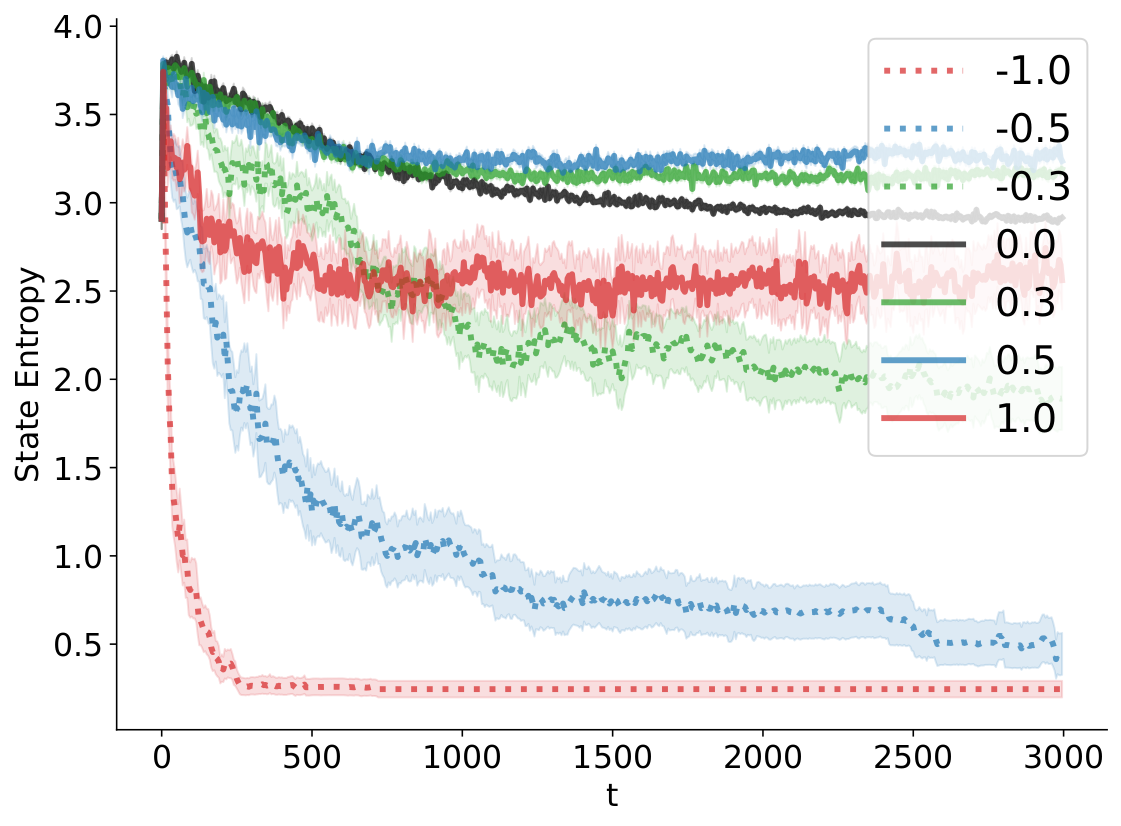
\includegraphics[width=\textwidth]{articles/baselines/figs/baseline_4rooms/NPG_state_entropy.png}
    \caption{Entropy (S)}
    \label{fig:4rooms_state}
  \end{subfigure}
  \caption{We plot the discounted returns, the entropy of the policy over the states visited in each trajectory, and the entropy of the state visitation distribution, averaged over 50 runs, for multiple baselines. The baselines are of the form $b(s) = b^*(s) + \epsilon$, perturbations of the minimum-variance baseline, with $\epsilon$ indicated in the legend. The shaded regions denote one standard error. Note that the policy entropy of lower baselines tends to decay faster than for larger baselines. Also, smaller baselines tend to get stuck on suboptimal policies, as indicated by the returns plot. See text for additional details.~\label{fig:stats_4rooms}}
\end{figure*}
We focused our theoretical analyses on multi-arm bandits so far. However, we are also interested in more general environments where gradient-based methods are commonplace. 
We now turn our attention to the Markov Decision Process (MDP) framework~\citep{puterman2014markov}. An MDP is a set $\{\gS, \gA, P, r, \gamma, \rho\}$ where $\gS$ and $\gA$ are the set of states and actions, $P$ is the environment transition function,
$r$ is the reward function, $\gamma \in [0, 1)$ the discount factor,
and $\rho$ is the initial state distribution. The goal of RL algorithms is to find a policy $\pi_\theta$, parameterized by $\theta$, which maximizes the (discounted) expected return; i.e. Eq.~\ref{eq:bandit_loss} becomes
\begin{align*}
    \arg\max_\theta \gJ(\theta)
    = \arg\max_\theta \sum_s d^{\pi_\theta}_\gamma(s)\sum_{a} \pi_\theta(a | s) r(s, a), %
\end{align*}
where there is now a discounted distribution over states induced by $\pi_\theta$. Although that distribution depends on $\pi_\theta$ in a potentially complex way, the parameter updates are similar to Eq.~\ref{eq:mc_update}:
\begin{align*}
    \theta_{t+1} &= \theta_t + \frac{\alpha}{N} \sum_i [Q(s_i, a_i) - b(s_i)]\nabla_\theta \log \pi_\theta(a_i | s_i) \label{eq:mc_update_mdp} \; ,
\end{align*}
where $(a_i, s_i)$ pairs are drawn according to the discounted state-visitation distribution induced by $\pi_\theta$ and $Q$ is the state-action value function induced by $\pi_\theta$~\citep[c.f.][]{sutton18book}. To match the bandit setting and common practice, we made the baseline state dependent. 

Although our theoretical analyses do not easily extend to multi-step MDPs, we empirically investigated if the similarity between these formulations leads to similar differences in learning dynamics when changing the baseline. We consider a 10x10 gridworld consisting of 4 rooms as depicted on Fig.~\ref{fig:4rooms_mdp}. We use a discount factor $\gamma=0.99$. The agent starts in the upper left room and two adjacent rooms contain a goal state of value $0.6$ or $0.3$. The best  goal (even discounted), with a value of $1$, lies in the furthest room, so that the agent must learn to cross the sub-optimal rooms and reach the furthest one. 

Similar to the bandit setting, for a state $s$, we can derive the minimum-variance baseline $b^*(s)$ assuming access to state-action values $Q(s,a)$ for $\pi_\theta$ and consider perturbations to it. Again, we use baselines $b(s) = b^*(s) + \epsilon$ and $b(s) = b^*(s) - \epsilon$, since they result in identical variances (this would not be the case if we used standard REINFORCE). 
We use a natural policy gradient estimate, which substitutes $\nabla \log \pi (a_i|s_i)$ by $F^{-1}_{s_i} \nabla \log \pi(a_i|s_i)$ in the update rule, where $F_{s_i}$ is the Fisher information matrix for state $s_i$ and solve for the exact $Q(s,a)$ values using dynamic programming for all updates (see Appendix \ref{app:npg_mdp_estimate} for details). 


In order to identify the committal vs. non-committal behaviour of the agent depending on the baseline, we monitor the entropy of the policy and the entropy of the stationary state distribution over time.
Fig.\ref{fig:4rooms_return} shows the average returns over time and Fig.\ref{fig:4rooms_action} and \ref{fig:4rooms_state} show the entropy of the policy in two ways. The first is the average entropy of the action distribution along the states visited in each trajectory, and the second is the entropy of the distribution of the number of times each state is visited up to that point in training.

The action entropy for smaller baselines tends to decay faster compared to larger ones, indicating convergence to a deterministic policy. This quick convergence is premature in some cases since the returns are not as high for the lower baselines.
In fact for $\epsilon=-1$, we see that the agent gets stuck on a policy that is unable to reach any goal within the time limit, as indicated by the returns of $0$.  
On the other hand, the larger baselines tend to achieve larger returns with larger entropy policies, but do not fully converge to the optimal policy as evidenced by the gap in the returns plot. 



Since committal and non-committal behaviour can be directly inferred from the PG and the sign of the effective rewards $R(\tau) - b$, we posit that these effects extend to all MDPs.
In particular, in complex MDPs, the first trajectories explored are likely to be suboptimal and a low baseline will increase their probability of being sampled again, requiring the use of techniques such as entropy regularization to prevent the policy~from~getting~stuck~too~quickly. 
In some preliminary experiments with a deep RL policy gradient algorithm, PPO \cite{schulman2017proximal}, where we perturb the baseline by a fixed constant, seem to indicate that negative perturbations perform slightly worse than positive perturbations. The results are not conclusive though and there are many confounding factors in this setting which could affect the outcome, including clipping due to PPO, neural network generalization, and adaptive optimizers. It is likely that a more careful strategy to perturb the baseline is needed to gain benefits, similar to using exploration bonuses. 

\section{Conclusion} 

We presented results that dispute common beliefs about baselines, variance, and policy gradient methods in general. 
As opposed to the common belief that baselines only provide benefits through variance reduction, we showed that they can significantly affect the optimization process in ways that cannot be explained by the variance and that lower variance can even sometimes be detrimental.

Different baselines can give rise to very different learning dynamics, even when they reduce the variance of the gradients equally. They do that by either making a policy quickly tend towards a deterministic one (\emph{committal} behaviour) or by maintaining high-entropy for a longer period of time (\emph{non-committal} behaviour). We showed that \textit{committal} behaviour can be problematic and lead to convergence to a suboptimal policy. Specifically, we showed that stochastic natural policy gradient does not always converge to the optimal solution due to the unusual situation in which the iterates converge to the optimal policy in expectation but not almost surely. 
Moreover, we showed that baselines that lead to lower-variance can sometimes be detrimental to optimization, highlighting the limitations of using variance to analyze the convergence properties of these methods. 
We also showed that standard convergence guarantees for PG methods do not apply to some settings because the assumption of bounded variance of the updates is violated.

The aforementioned convergence issues are also caused by the problematic coupling between the algorithm's updates and its sampling distribution since one directly impacts the other. As a potential solution, we showed that off-policy sampling can sidestep these difficulties by ensuring we use a sampling distribution that is different than the one induced by the agent's current policy. This supports the hypothesis that on-policy learning can be problematic, as observed in previous work~\citep{schaul2019ray, hennes2020neural}. Nevertheless, importance sampling in RL is generally seen as problematic~\citep{vanHasselt2018deadly_triad} due to instabilities it introduces to the learning process. Moving from an imposed policy, using past trajectories, to a chosen sampling policy reduces the variance of the gradients for near-deterministic policies and can lead to much better behaviour. In general, other variance-reduction strategies may also be more effective \cite{xu2019sample}.

More broadly, this work suggests that treating bandit and reinforcement learning problems as a black-box optimization of a function $\gJ(\theta)$ may be insufficient to perform well. As we have seen, the current parameter value can affect all future parameter values by influencing the data collection process and thus the updates performed. Theoretically, relying on immediately available quantities such as the gradient variance and ignoring the sequential nature of the optimization problem is not enough to discriminate between certain optimization algorithms. In essence, to design highly-effective policy optimization algorithms, it may be necessary to develop a better understanding of how the optimization process evolves over many steps. 


\section*{Acknowledgements}
We would like to thank Kris de Asis, Alan Chan, Ofir Nachum, Doina Precup, Dale Schuurmans, and Ahmed Touati for helpful discussions. We also thank Courtney Paquette, Vincent Liu, Scott Fujimoto and Csaba Szepesv\'{a}ri for reviewing an earlier version of this paper. Marlos C. Machado and Nicolas Le Roux are supported by a Canada CIFAR AI Chair.







 \chapter*{Conclusion}

In this thesis, we have explored the roles and challenges presented by
stochasticity in reinforcement learning and optimization algorithms. We have
investigated the impact of noise in the learning process and presented four significant contributions that address various aspects of this issue.
The main axes of our research were the following:

        \val{Not sure about the name of this first point}
\begin{itemize}
    \item \textbf{Learning diverse behaviors for planning:}
        Our first two articles focused on learning stochastic policies able to
        explore the environment and discover diverse behaviors. In our first
        article, \emph{Independently Controllable Factors}, we learn policies,
        or options, indexed on a latent factor representation $z$. We were able
        to show that we both learned disentangled representations of the world
        as well as policies that were able to modify these factors. Finally, we
        were able to demonstrate how this representation could be used for
        planning.
        In our second article, \emph{Sequential Monte Carlo Planning}, we
        designed a general purpose planning algorithm that can be used in
        continuous control tasks. Our SMCP algorithm can be viewed as a maximum
        entropy planning algorithm and as such can discover stochastic policies
        discovering diverse solutions.
    \item \textbf{Understanding the role of noise:} The next two contributions
        were more focused on understanding the role of noise during the
        optimization process. In our third article, we analyse the role of the
        interplay between the gradient noise and the local curvature of the loss
        function. Specifically, we show it can impact the optimization speed and
        generalization properties of models trained via maximum likelihood.
        Finally, in our fourth article, we investigate the role of
        \emph{baselines} in policy gradient methods. Baselines are often
        presented as a way to reduce the variance of the gradient estimator
        without affecting the bias. We show that baselines have an effect beyond
        variance reduction directly impact the
        exploration/exploitation trade-off and as such can impact which policies
        are discovered.
\end{itemize}


The work presented in this thesis provides valuable insights into the role of stochasticity in reinforcement learning and optimization algorithms, offering a solid foundation for future research in this area.

By further examining the interplay between noise and learning, we can continue to develop more robust, adaptive, and efficient algorithms that can better handle the challenges of real-world environments. Ultimately, understanding and harnessing the power of stochasticity will bring us closer to achieving the long-term goal of creating intelligent machines capable of interacting with the world and learning from experience, just as humans and animals do.




 
 












\bibliographystyle{icml2018}
\def\bibname{R\'ef\'erences bibliographiques} %
\bibliography{references}




\appendix
\chapter{Appendix A}
\section{Additional details}
\subsection{Architecture}
Our architecture is as follows: the encoder, mapping the raw pixel state to a latent representation, is a 4-layer convolutional neural network with batch normalization \citep{ioffe2015batch} and leaky ReLU activations. The decoder uses the transposed architecture with ReLU activations. The noise $z$ is sampled from a 2-dimensional gaussian distribution and both the generator $\Phi(h,z)$ and the policy $\pi(h,\phi)$ are neural networks consisting of 2 fully-connected layers. In practice, a minibatch of $n = 256$ or $1024$ vectors $\phi_1, \dots, \phi_{n}$ is sampled at each step. The agent randomly choses one $\phi = \phi_{behavior}$ and samples actions from its policy $a \sim \pi(h, \phi_{behavior})$. Our model parameters are then updated using policy gradient with the REINFORCE estimator and a state-dependent baseline and importance sampling. For each selectivity reward, the term $\mathbb{E}_{\phi'}[  A(h', h,\phi')]$ is estimated as $\tfrac{1}{n} \sum_{i = 1}^n A(h', h,\phi_i)$.

In practice, we don't use concatenation of vectors when feeding two vectors as input for a network (like $(h, z)$ for the factor generator or $(h, \phi)$ for the policy).
For vectors $a,b \in \mathbb{R}^{n_a \times n_b}$. We use a bilinear operation $bil(a, b) = (a_i * b_j)_{i \in [[n_a]], j \in [[n_b]]}$ as in \cite{florensa2017stochastic}.  We observe the bilinear integrated input to more strongly enforce dependence on both vectors; in contrast, our models often ignored one input when using a simple concatenation.

Through our research, we experiment with different outputs for our generator $\Phi(h,z)$.  We explored embedding the $\phi$-vectors into a hypercube, a hypersphere, a simplex and also a simplex multiplied by the output of a $tanh(\cdot)$ operation on a scalar.

\subsection{First experiment}
In the first experiment, figure~\ref{fig:dis_space}, we used a gaussian similarity kernel i.e $A(h', h, \phi) = \exp(- \frac{||h' - (h+\phi)||^2}{2 \sigma^2})$ with $\sigma = \sqrt{dim(h)}$.
In this experiment only, for clarity of the figure, we only allowed permissible actions in the environment (no no-op action).


% Our attribute selector $A(dh, \phi)$ is a gaussian kernel.

\section{Additional Figures}
\subsection{Discrete simple case}
\label{sec:sel-only}
Here we consider the case where we learn a latent space $H$ of size $K$, with $K$ factors corresponding to the coordinates of $h$ ($h_i,\; i\in[k])$, and learn $K$ separately parameterized policies $\pi_i(a|h),\;i\in[k]$. We train our model with the selectivity objective, but no autoencoder loss, and find that we correctly recover independently controllable features on a simple environment.
{%We also find experimentally that training discrete independently controllable features without training the autoencoder objective correctly recovers ground truth features and their associated control policies. 
Albeit slower than when jointly training an autoencoder, this shows that the objective we propose is strong enough to provide a learning signal for discovering a disentangled latent representation.
}

{We train such a model on a gridworld MNIST environment, where there are two MNIST digits \nocite{lecun1998mnist}. The two digits can be moved on the grid via 4 directional actions (so there are 8 actions total), the first digit is always odd and the second digit always even, so they are distiguishable. In Figure \ref{fig:gridworld-only-sel} we plot each latent feature $h_k$ as a curve, as a function of each ground truth. For example we see that the black feature recovers $+x_1$, the horizontal position of the first digit, or that the purple feature recovers $-y_2$, the vertical position of the second digit.}
\begin{figure}[H]
\centering
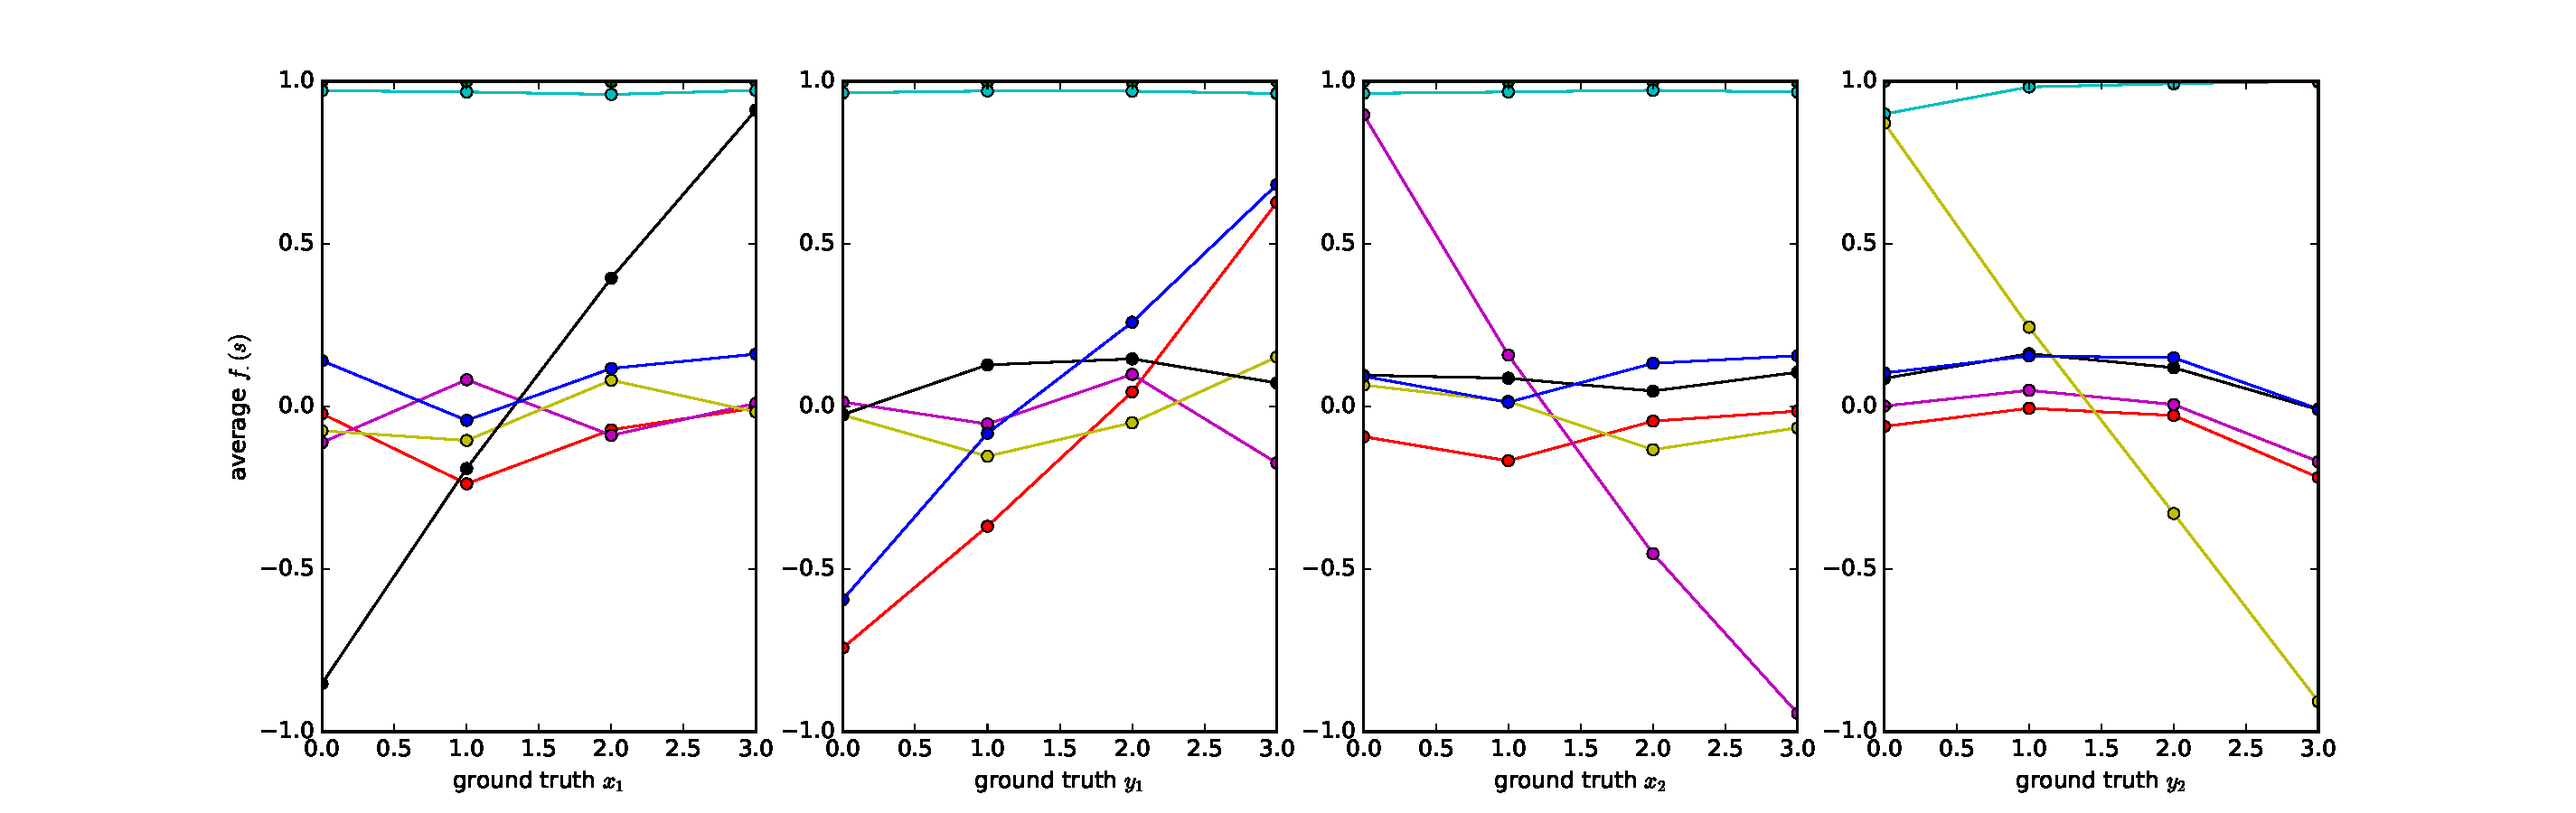
\includegraphics[width=\linewidth]{articles/icf/figures/latent_vs_gt_005.pdf}
\caption{{%Each curve represents a latent feature $f_k$ as a function of some ground truth. Here there are 4 ground truths, the $x$ and $y$ position of each of the 2 MNIST digits.
In a gridworld environment with 2 objects (in this case 2 MNIST digits), we know there are 4 underlying features, the $(x_i,y_i)$ position of each digit $i$. Here each of the four plots represents the evolution of the $f_k$'s as a function of their underlying feature, from left to right $x_1$, $y_1$, $x_2$, $y_2$. We see that for each of them, at least one $f_k$ recovers it almost linearly, from the raw pixels only.}
}
\label{fig:gridworld-only-sel}
\end{figure}


\subsection{Planning and policy inference example in 1-step}
\label{sec:exp-mb-ppi}

This disentangled structure could be used to address many challenging issues in reinforcement learning. We give two examples in figure~\ref{fig:prediction_recovering}: 
\begin{itemize}
\item Model-based predictions: Given an initial state, $s_0$, and an action sequence $a_{\{0:T-1\}}$, %the agent performed, our goal is to predict the resulting state $s_T$.
we want to predict the resulting state $s_T$.

\item A simplified deterministic policy inference problem: Given an initial state $s_{start}$ and a terminal state $s_{goal}$, we aim to find a suitable action sequence $a_{\{0:T-1\}}$ such that $s_{goal}$ can be reached from $s_{start}$ by following it.
\end{itemize}
Because of the $tanh$ activation on the last layer of $\Phi(h, z)$, the different factors of variation $dh = h' - h$ are placed on the vertices of a hypercube of dimension $K$, and we can think of the the policy inference problem as finding a path in that simpler space, where the starting point is $h_{start}$ and the goal is $h_{goal}$. We believe this could prove to be a much easier problem to solve.

\begin{figure}[H]
\centering
\subfloat[]{\scalebox{.6}{
\begin{tikzpicture}
\node[inner sep=0pt] (im0) at (0,0)
    {\fbox{
\includegraphics[width=.25\textwidth]{articles/icf/figures/im0_good.png}}};
\node[inner sep=0pt] (im1) at (5,0)
    {\fbox{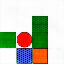
\includegraphics[width=.25\textwidth]{articles/icf/figures/im1_good.png}}};


\node[] (ht) at (0,-4) {$\underbrace{h}_{(0.4,\ 13.1)}$};
\node[] (ht1) at (7,-4) {$\underbrace{\hat{h'}}_{(-4.6,\ -1.9)} = h + \underbrace{dh_{{\color{right} {\color{right} right}}}}_{(5,\ -5)} + \underbrace{2\cdot dh_{{\color{down} down}}}_{(-10,\ -10)}$}; 
    \draw[->,thick] (im0.south) -- (ht.north)
    node[midway,fill=white] {Encoder};
    \draw[->,thick] (5, -3.3) -- (im1.south)
    node[midway,fill=white] {Decoder};
    
    \draw[->,thick] (ht.east) -- (ht1.west);
    
\end{tikzpicture}}}
\hfill
%\subfloat[]{\includegraphics[width=.3\linewidth]{./images/pdoth_tsne_p.png}}
\subfloat[]{\scalebox{.6}{
\begin{tikzpicture}
\node[inner sep=0pt] (im0) at (0,0)
    {\fbox{
\includegraphics[width=.25\textwidth]{articles/icf/figures/im_causal0_good.png}}};
\node[inner sep=0pt] (im1) at (5,0)
    {\fbox{
\includegraphics[width=.25\textwidth]{articles/icf/figures/im_causal1_good.png}}};


\node[] (ht) at (0,-3.5) {$\underbrace{h_1}_{(0.4,\ 13.1)}$};
\node[] (ht1) at (5,-3.5) {$\underbrace{h_2}_{(5.9,\ -11.6)}$}; 
\node[] (dh) at (2.5,-5) {$dh ={(5.5,\ -24.8)} \approx 2\cdot dh_{{\color{down} down}} + 3\cdot dh_{{\color{right} right}}$};
    \draw[->,thick] (im0.south) -- (ht.north)
    node[midway,fill=white] {Encoder};
    \draw[<-,thick] (ht1) -- (im1.south)
    node[midway,fill=white] {Encoder};
    
    \draw[->,thick] (ht.east) -- (dh.north);
     \draw[->,thick] (ht1.west) -- (dh.north);
    
\end{tikzpicture}}
} %trim={0px 0 0px 0},clip
\caption{(a) Predicting the effect of a cause on Mazebase. The leftmost image is the visual input of the environment, where the agent is the round circle, and the switch states are represented by shades of green. After the training, we are able to distinguish one cluster per $dh$ (Figure \ref{fig:dis_space}), that is to say per variation obtained after performing an action, independently from the position $h$. Therefore, we are able to move the agent just by adding the corresponding $dh$ to our latent representation $h$. The second image is just the reconstruction obtained by feeding the resulting $h'$ into the decoder. (b) Given a starting state and a goal state, we are able to decompose the difference of the two representations $dh$ into a (non-directed) sequence of movements.}
\label{fig:prediction_recovering}
\end{figure}

\subsection{Multistep Example}
\label{sec:multistep}
We demonstrate an instance of ICF operating in a 4$\times$4 Mazebase enviroment over five time steps in Figure \ref{fig:multistep_toggle}. We consistently witness a failure of mode collapse in our generator $\Phi$ and therefore the generator only produces a subset of all possible $\phi$-variations.  In Figure \ref{fig:multistep_toggle}, we observe the $\phi$ governing the agent's policy $\pi_{\phi}$ appears to correspond to moving two positions down and then to repeatedly toggle the switch.  A random action due to $\epsilon$-greedy led to the agent moving up and off the switch at time step-4. This perturbation is corrected by the policy $\pi_{\phi}$ by moving down in order to return to toggling the relevant switch.

\begin{figure}[H]
\centering
\subfloat[]{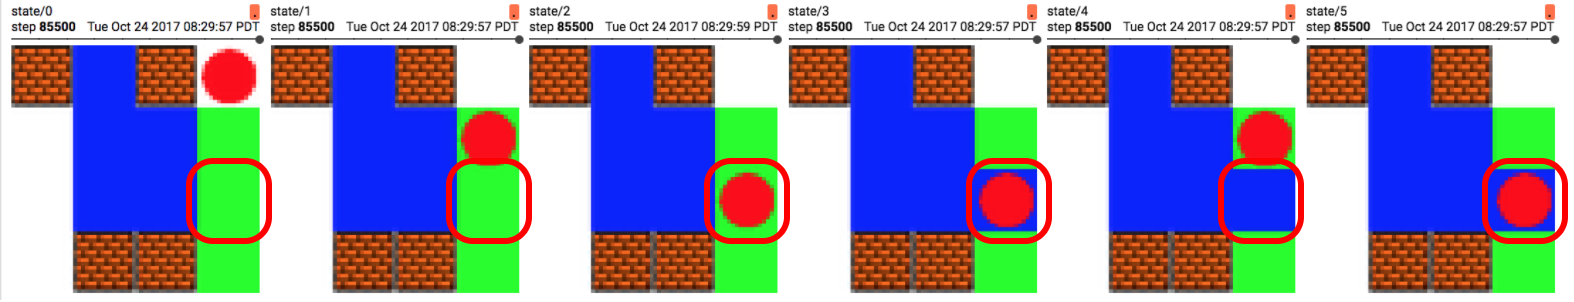
\includegraphics[width=.8\linewidth]{articles/icf/figures/ex1_env_5_step_boxed.png}}
\newline
\subfloat[]{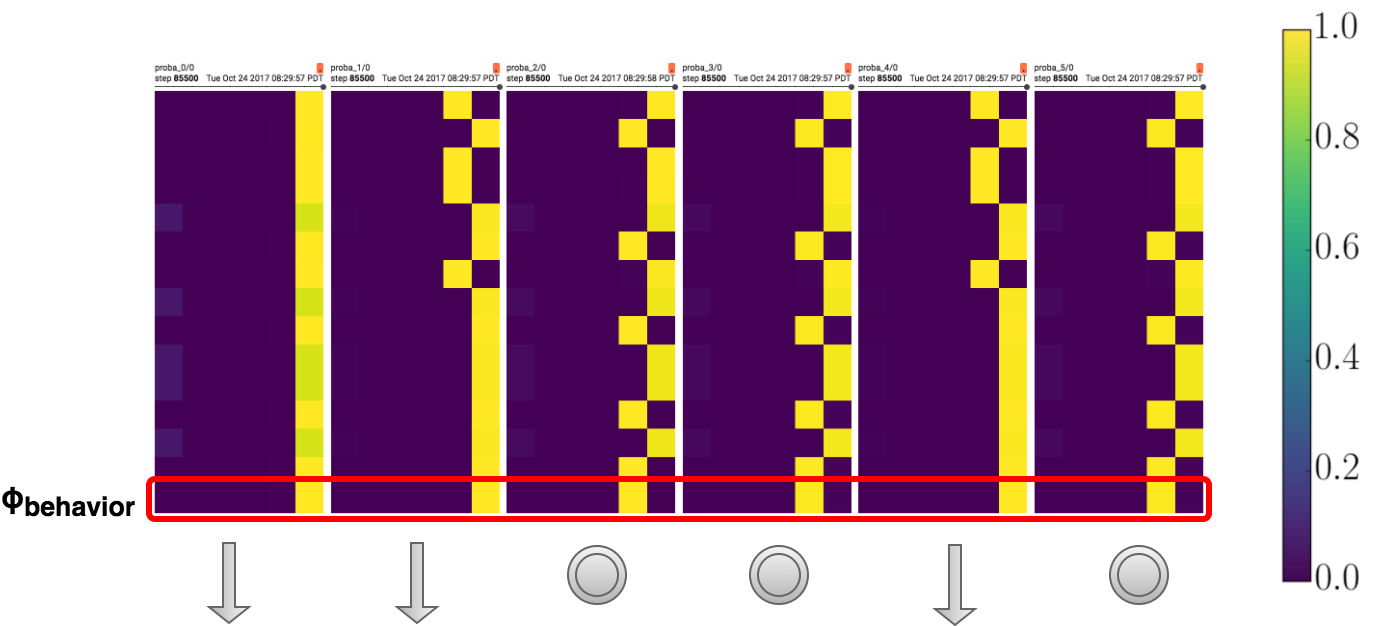
\includegraphics[width=.8\linewidth]{articles/icf/figures/ex1_action_probs_5_step_denoted_boxed.png}} 
\caption{(a) Mazebase environment over five time-steps.  Here the red dot denotes the position of the agent.  The $\phi_{behavior}$ governing the agent's policy appears to control toggling the switch indicated by the red rounded box. 
(b) Visualization of the policies instantiated by different $\phi$s.  Each box represents the probability distribution of the policies at that time step.  Each row is generated by a different $\phi$ and each column corresponds to an action (up, left, pass, right, toggle, down) in order.  The boxed column shows the $\phi_{behavior}$. The symbols below each box represent the most-probable action for the behavioral policy, where the grey circle indicates toggling the switch.}
\label{fig:multistep_toggle}
\end{figure}



\section{Variational bound and the selectivity}
\label{appendix:bound}
% \begin{tikzpicture}
\tikzstyle{main}=[circle, minimum size = 5mm, thick, draw =black!80, node distance = 7mm]
\tikzstyle{connect}=[-latex, thick]
\tikzstyle{box}=[rectangle, draw=black!100]
  \node[box,draw=white!100] (Latent) {\textbf{Latent}};
  \node[main] (a1) [right=of Latent] {$\va_1$};
  \node[main] (s1) [below=of a1] {$\vs_1$};
  \node[draw,thick, rounded corners, fit=(s1) (a1)] (L1) {};
  \node[main] (a2) [right=of a1] {$\va_2$};
  \node[main] (s2) [below=of a2] {$\vs_2$};
  \node[draw,thick, rounded corners, fit=(s2) (a2)] (L2) {};
  \node[main] (a3) [right=of a2] {$\va_3$};
  \node[main] (s3) [below=of a3] {$\vs_3$};
  \node[draw,thick, rounded corners, fit=(s3) (a3)] (L3) {};
  \node[main] (at) [right=of a3] {$\va_t$};
  \node[main] (st) [below=of at] {$\vs_t$};
  \node[draw,thick, rounded corners, fit=(st) (at)] (Lt) {};
  
  
  \node[box,draw=white!100] (Observed) [above=of Latent] {\textbf{Observed}};
  \node[main,fill=black!10] (O1) [right=of Observed,above=of L1] {$\gO_1$};
  \node[main,fill=black!10] (O2) [right=of O1,above=of L2] {$\gO_2$};
  \node[main,fill=black!10] (O3) [right=of O2,above=of L3] {$\gO_3$};
  \node[main,fill=black!10] (Ot) [right=of O3,above=of Lt] {$\gO_t$};

  \path (L3) -- node[auto=false]{\ldots} (Lt);
  \path (a1) edge [connect] (O1)
        (s1) edge [connect, bend right=45] (O1)
        (s1) edge [connect] (s2)
        (a1) edge [connect] (s2);
    \path (a2) edge [connect] (O2)
        (s2) edge [connect, bend right=45] (O2)
        (s2) edge [connect] (s3)
        (a2) edge [connect] (s3);
  \path (a3) edge [connect] (O3)
        (s3) edge [connect, bend right=45] (O3);
  \path (at) edge [connect] (Ot)
        (st) edge [connect, bend right=45] (Ot);
  \path (L3) -- node[auto=false]{\ldots} (Lt);

  \draw[dashed]  [below=of L1,above=of O1];
\end{tikzpicture}
Let us call $p(h_{t+1} | \phi_{t+1}, h_t) =  \mathcal{P}^\phi_{h' ,h}$ the probability distribution over final hidden states starting from $h$ and using the policy parametrized by the embedding $\phi$.

$p(h_{t+1} | \phi_{t+1}, h_t) = \Pi_{k=1}^{K}  \pi_{\phi_{t+1}}( a_{t+\frac{k-1}{K}} | h_{t+\frac{k-1}{K}}) p_{env}(s_{t+\frac{k}{K}} | a_{t+\frac{k-1}{K}}, s_{t+\frac{k-1}{K}})$.
where $p_{env}$ is the transition probability of the environment.
% $p(\bullet | \phi, h)$ 

For simplicity, let's refer to $h_t$ as $h$, $h_{t+1}$ as $h'$ and $\phi_{t+1}$ as $\phi$.
\subsection{Lower bound on the mutual information}
The bound $$\mathcal{I}_p(\phi, h' | h) \ge \sup_\theta  \mathbb{E}_{p(\phi|h)} \big[ \mathcal{S}(h, \phi)\big]$$ can be proven by using Donsker-Varadhan variational representation of the KL divergence \citep{donsker1975asymptotic,ruderman2012tighter}:

$$\kl{p}{q} = \sup_{T \in \mathcal{L}^\infty(q)} \mathbb{E}_p \big[ T  \big] - \log \mathbb{E}_q \big[ e^T \big]$$

For $A = e^T$ and using the identity $\mathcal{I}_p(X, Y) = \mathbb{E}_{p(y)} \big[ \kl{p(x|y)}{p(x)}\big]$ with $X=\phi|h$ and $Y=h'|h$, we have:

\begin{eqnarray*}
\mathcal{I}_p(\phi, h' | h) &=& \mathbb{E}_{h'|h} \sup_A \mathbb{E}_{\phi|h, h'} \big[ \log A(h', h, \phi) \big] - \log \mathbb{E}_{\varphi|h} \big[ A(h', h, \varphi) \big]\\
&=& \mathbb{E}_{h'|h} \sup_A \mathbb{E}_{\phi|h, h'} \big[ \log \frac{ A(h', h, \phi)}{\mathbb{E}_{\varphi|h} \big[ A(h', h, \varphi)\big]}\big]\\
&\ge&  \sup_A \mathbb{E}_{\phi|h}\mathbb{E}_{h'|\phi, h} \big[ \log \frac{ A(h', h, \phi)}{\mathbb{E}_{\varphi|h} \big[ A(h', h, \varphi)\big]}\big]\\
&\ge&  \sup_\theta \mathbb{E}_{\phi|h}\mathbb{E}_{h'|\phi, h} \big[ \log \frac{ A(h', h, \phi; \theta)}{\mathbb{E}_{\varphi|h} \big[ A(h', h, \varphi; \theta)\big]}\big]\\
\end{eqnarray*}
for parametric $A$ functions.

% In the case where $A(h', h, \phi)$ is actually is probability density $q(h' | h, \phi)$ (or any unnormalized density such that the normalization factor does not depend on $\phi$) we have:
% \begin{eqnarray*}
% \mathcal{S}(\phi, h) &=&\mathbb{E}_{h' \sim p
%     (h' | \phi, h)}  \log \frac{q(h' | \phi, h)}{\mathbb{E}_{\varphi | h} q(h' |
%     \varphi,
% h)}\\
% &=& \mathbb{E}_{\phi | h} \big[ {\kl{p(h'|\phi, h)}{q(h'|h)} -
% \kl{p(h'|\phi, h)}{q(h'|\phi, h)}} \big]\\
% &=& \mathbb{E}_{\phi | h} \big[ \kl{p(h'|\phi, h)}{q(h'|h)}\big] -
% \kl{p(h'| h)}{q(h'|h)} - \mathbb{E}_{p(h'|h)} \big[ \kl{p(\phi| h', h)}{q(\phi |h', h)}\big] \\
% &=& \mathbb{E}_{\phi | h} \big[ \kl{p(h'|\phi, h)}{p(h'|h)}\big]- \mathbb{E}_{p(h'|h)} \big[ \kl{p(\phi| h', h)}{q(\phi |h', h)}\big] \\
% &=& \mathcal{I}^{p} (\phi , h'|h) - \mathbb{E}_{p(h'|h)} \big[ \kl{p(\phi| h', h)}{q(\phi |h', h)}\big] \\
% % &=& \mathcal{I}^{p}(\phi \mapsto h')- \mathbb{E}_{p(h'|h)} \big[ \kl{p(\phi| h', h)}{q(\phi |h', h)}\big] \\
% \end{eqnarray*}
% where we used that fact that $p(\phi|h) = q(\phi|h)$ and by design we only sample $\phi$s from one generator.

% Thus, the gap between the selectivity and the mutual information is the KL divergence of the two posterior distributions.


As we sample the factors $\phi$ uniformly, our total objective is then a lower bound on $\sum_t \mathcal{I}(\phi_t, h_t | h_{t-1})$ which corresponds here to the \emph{directed information} \citep{massey1990causality} \cite{ziebart2010modeling} as $\phi_t$ is sampled independently from $\phi_{1:t-1}$.


% \input{equivariant_map.tex}


\section{Additional information on the training}

In our experiments, we use the selectivity objective, an autoencoding loss and an entropy regularization loss $\mathcal{H}(\pi_\phi)$ for each of the policies $\pi_\phi$. Furthermore, in experiment 4.2 we added the model-based cost $||h' - T(h, \phi)||^2$ with $T$ a learned two layer fully connected neural network.

The selectivity is used to update the parameters of the encoder, factor generator and policy networks.
We use the following equation for computing the gradients

$$\nabla_\theta \mathbb{E}_{\pi_\theta} \big[ f_\theta \big] =  \mathbb{E}_{\pi_\theta} \big[ \nabla_\theta f_\theta + f_\theta \nabla_\theta \log \pi_\theta \big]$$ 
We also use a state dependent baseline $V$ as a control variate to reduce the variance of the REINFORCE estimator.

Furthermore, to be able to train the factor generator efficiently, we train all $\phi$ sampled in a mini-batch (of size $1024$) by importance sampling on the probability ratio of the trajectory under each $\phi$

\chapter{SMCP appendix}
\section{Appendix}
\label{sec:appendix}

\subsection{Abbreviation and Notation}
\label{app:notation}
\begin{table}[H]\caption{Abbreviation}
\begin{center}% used the environment to augment the vertical space
% between the caption and the table
\begin{tabular}{r c p{10cm} }
\toprule
SMCP: & Sequential Monte Carlo Planning.\\
SAC: & Soft Actor Critic.\\
CEM: & Cross Entropy Method.\\
RS: & Random Shooting.\\
MCTS: & Monte Carlo Tree Search.\\
SMC: & Sequential Monte Carlo.\\
SIR: & Sequential Importance Resampling.\\
SIS: & Sequential Importance Sampling.\\
IS: & Importance Sampling.\\
MPC: & Model Predictive Control\\
\bottomrule
\end{tabular}
\end{center}
\label{tab:abbreviation}
\end{table}

\begin{table}[H]\caption{Notation}
\begin{center}% used the environment to augment the vertical space
% between the caption and the table
\begin{tabular}{r c p{10cm} }
\toprule
$\traj_{1:T}$ & $\triangleq$ & $\{\rvs_i, \rva_i\}_{i=1}^T$ the state-action pairs.\\
$V$  & $\triangleq$ & value function.\\
$\mathcal{O}_t$ & $\triangleq$ & Optimality variable.\\
$p(\mathcal{O}_t|\rvs_t, \rva_t)$ & $\triangleq$ & $\exp(r(\rvs_t, \rva_t))$ Probability of a pair state action of being optimal.\\
$\penv$ & $\triangleq$ & Transition probability of the environment. Takes state and action $(\rvs_t, \rva_t)$ as argument and return next state and reward $(\rvs_{t+1}, r_t)$.\\
$\pmodel$ & $\triangleq$ & Model of the environment. Takes state and action $(\rvs_t, \rva_t)$ as argument and return next state and reward $(\rvs_{t+1}, r_t)$.\\
% $w$ & $\triangleq$ & Unnormalized weight of the importance sampling.\\ 
% $\bar{w}$ & $\triangleq$ & Normalized weight of the importance sampling.\\
$w_t$ & $\triangleq$ & Importance sampling weight.\\ 
% $w_{t|T}$ & $\triangleq$ & Smoothing importance sampling weight.\\ 
$p(\traj)$  & $\triangleq$ & Density of interest.\\
$q(\traj)$  & $\triangleq$ & Approximation of the density of interest.\\
$t \in \{1, \ldots T\}$ & $\triangleq$ & time steps. \\
$n \in \{1, \ldots N\}$ & $\triangleq$ & particle number. \\
$h$ & $\triangleq$ & horizon length. \\
\bottomrule
\end{tabular}
\end{center}
\label{tab:notation}
\end{table}

%\subsection{Ablation Study}
%
%\begin{figure}
%    \centering
%    \includegraphics[angle=90,origin=c,scale=0.5]{ablation_study_halfcheetah}
%    \caption{Ablation study on half cheetah.}
%    \label{fig:my_label}
%\end{figure}

\subsection{The action prior}
\label{app:action_prior}

The true joint distribution~\ref{eq:posterior_target} in section~\ref{sec:control_as_inference} should actually be written:
\begin{eqnarray*}
\label{eq:true_posterior_target}
p(\traj_{1:T}, \gO_{1:T}) &=& \mu(\rvs_1) \prod_{t=1}^{T-1} \penv(\rvs_{t+1}|\rva_t, \rvs_t) \prod_{t=1}^{T} p(\rva_t) \exp\big(\sum_{t=1}^{T} r(\rvs_t, \rva_t)\big) \\
&=& \mu(\rvs_1) \prod_{t=1}^{T-1} \penv(\rvs_{t+1}|\rva_t, \rvs_t)\exp\big(\sum_{t=1}^{T} r(\rvs_t, \rva_t) + \log p(\rva_t)\big) \\
\end{eqnarray*}
In Mujoco environments, the reward is typically written as 
$$r(\rvs_t, \rva_t) = f(\rvs_t) - \alpha ||\rva_t||_2^2 $$
where $f$ is a function of the state (velocity for HalfCheetah on Mujoco for example). The part $\alpha ||\rva_t||_2^2$ can be seen as the contribution from the action prior (here a gaussian prior).
One can also consider the prior to be constant (and potentially improper) so that is does not change the posterior $p(\traj_{1:T}| \gO_{1:T})$.

% \subsection{Recursive filtering weights}

% \label{app:rec_weights}
% \begin{align}
% w_t &= \frac{p(\traj_{1:t} | \gO_{1:t})}{q(\traj_{1:t})} \nonumber\\
% &= \frac{p(\traj_{1:t-1} | \gO_{1:t-1}) \penv(\rvs_{t+1} | \rvs_t, \rva_t) p(\gO_t | \rvs_t, \rva_t)}{q(\traj_{1:t-1}) q(\traj_t | \traj_{1:t-1})} \nonumber\\
% &= \frac{p(\traj_{1:t-1} | \gO_{1:t-1}) }{q(\traj_{1:t-1}) }\frac{\penv(\rvs_{t+1} | \rvs_t, \rva_t) \exp(r_t)}{\pmodel(\rvs_{t+1} | \rvs_t, \rva_t) \pi_\parampol(\rva_t | \rvs_t)} \nonumber\\
% &= w_{t-1}\frac{\penv(\rvs_{t+1} | \rvs_t, \rva_t)}{\pmodel(\rvs_{t+1} | \rvs_t, \rva_t) } \exp(r_t - \log \pi_\parampol(\rva_t | \rvs_t))
% \end{align}

\subsection{Value function: backward message}
 \label{app:backward_message}
\begin{align}
    p(\gO_{t+1:T} | \traj_t) &=  \int_{\traj_{t+1}} p(\gO_{t+1:T}, \traj_{t+1} | \traj_t)d\traj_{t+1} \nonumber\\
     &=  \int_{\traj_{t+1}} p(\traj_{t+1} | \traj_{t}, \gO_{t+1:T}) p(\gO_{t+1:T} | \traj_{t+1}) d\traj_{t+1}  \nonumber\\
    % &= \int_{\traj_{t+1}} p(\traj_{t+1}|\traj_t) \exp Q(\rvs_{t+1}, \rva_{t+1}) d\traj_{t+1} \nonumber\\
     &= \int_{\rvs_{t+1}}  \penv(\rvs_{t+1} | \rvs_t, \rva_t) \left[ \int_{\rva_{t+1}} p(\rva_{t+1} | \rvs_{t+1}, \gO_{t+1:T}) \exp Q(\rvs_{t+1}, \rva_{t+1}) d\rva_{t+1}  \right] d\rvs_{t+1}\nonumber\\
     &= \int_{\rvs_{t+1}} \penv(\rvs_{t+1} | \rvs_t, \rva_t)  \exp \big( V(\rvs_{t+1}) \big) d\rvs_{t+1}\nonumber\\
       &= \E_{\rvs_{t+1} | \rvs_t, \rva_t} [ \exp \big( V(\rvs_{t+1}) \big)]
\end{align}
By definition of the optimal value function in~\citep{levine2018reinforcement}.


\subsection{Recursive weights update}
% {\color{red} Version with Q function}
% For this derivation, we need the forward backward equation
% \begin{align}
%     {p(\traj_{1:t} | \gO_{1:T})} & \propto \mathunderline{alpha}{p(\traj_{1:t}|\gO_{1:t})} \cdot \mathunderline{beta}{p(\gO_{t+1:T}|\traj_{t})}
% \end{align}
% and its alternative form
% \begin{align}
%     {p(\traj_{1:t} | \gO_{1:T})} & \propto \mathunderline{alpha}{p(\traj_{1:t}|\gO_{1:t-1})} \cdot \mathunderline{beta}{p(\gO_{t:T}|\traj_{t})}
% \end{align}


\label{app:rec_weights}
\begin{align}
w_t &= \frac{p(\traj_{1:t} | \gO_{1:T})}{q(\traj_{1:t})} \nonumber\\
&= \frac{p(\traj_{1:t-1} | \gO_{1:T})}{q(\traj_{1:t-1})}\frac{p(\traj_t |\traj_{1:t-1}, \gO_{1:T})}{q(\traj_t | \traj_{1:t-1})} \nonumber\\
&= w_{t-1} \cdot \frac{p(\traj_t |\traj_{1:t-1}, \gO_{1:T})}{q(\traj_t | \traj_{1:t-1})} \nonumber\\
&= w_{t-1} \frac{1}{ q(\traj_t | \traj_{1:t-1})} \frac{p(\traj_{1:t} | \gO_{1:T})}{ p(\traj_{1:t-1} | \gO_{1:T})} \nonumber\\
&\text{We use there the forward-backward equation~\ref{eq:forwardbackward} for the numerator and the denominator} \nonumber\\
 &\propto w_{t-1}   \frac{1}{ q(\traj_t | \traj_{1:t-1})} \frac{ \textcolor{orange}{p(\traj_{1:t} | \gO_{1:t})}}{ \textcolor{orange}{p(\traj_{1:t-1} | \gO_{1:t-1})}} \frac{ \textcolor{beta}{p(\gO_{t+1:T} | \traj_{t})}}{ \textcolor{beta}{p(\gO_{t:T} | \traj_{t-1})}}   \nonumber\\
&= w_{t-1}   \frac{ p(\traj_t | \traj_{1:t-1})}{ q(\traj_t | \traj_{1:t-1})}  p(\gO_t | \traj_t)   \frac{ p(\gO_{t+1:T} | \traj_{t})}{ p(\gO_{t:T} | \traj_{t-1})}  \nonumber\\
&= w_{t-1}    \frac{\penv(\rvs_{t} | \rvs_{t-1}, \rva_{t-1})}{ \pmodel(\rvs_{t} | \rvs_{t-1}, \rva_{t-1}) }   \frac{\exp (r_t)}{\pi_\parampol(\rva_t|\rvs_t)} \frac{\E_{\rvs_{t+1} | \rvs_t, \rva_t} [ \exp \big( V(\rvs_{t+1}) \big)] }{\E_{\rvs_{t} | \rvs_{t-1}, \rva_{t-1}} [ \exp \big( V(\rvs_{t}) \big)]}  \nonumber\\
% &= \frac{p(\traj_{1:t-1} | \gO_{1:t-1}) }{q(\traj_{1:t-1}) }\frac{\penv(\rvs_{t+1} | \rvs_t, \rva_t) \exp(r_t)}{\pmodel(\rvs_{t+1} | \rvs_t, \rva_t) \pi_\parampol(\rva_t | \rvs_t)} \nonumber\\
% &= w_{t-1}\frac{\penv(\rvs_{t+1} | \rvs_t, \rva_t)}{\pmodel(\rvs_{t+1} | \rvs_t, \rva_t) } \exp(r_t - \log \pi_\parampol(\rva_t | \rvs_t))
&= w_{t-1} \frac{\penv(\rvs_{t} | \rvs_{t-1}, \rva_{t-1})}{ \pmodel(\rvs_{t} | \rvs_{t-1}, \rva_{t-1}) }  \E_{\rvs_{t+1} | \rvs_t, \rva_t} [ \exp \big( r_t  -  \log \pi_\parampol(\rva_t | \rvs_t) + V(\rvs_{t+1}) - \log \E_{\rvs_{t} | \rvs_{t-1}, \rva_{t-1}} [ \exp \big( V(\rvs_{t}) \big)] \big)]
\end{align}


% As 
% $$p(\traj_{1:t} | \gO_{1:t}) = \mu(\rvs_1) \prod_{\tau=1}^{t-1} \penv(\rvs_{\tau+1}|\rva_\tau, \rvs_\tau) \exp\big(\sum_{\tau=1}^{t} r(\rvs_\tau, \rva_\tau) + \log p(\rva_\tau) \big)$$
% We have
% $$\frac{p(\traj_{1:t} | \gO_{1:t})}{ p(\traj_{1:t-1} | \gO_{1:t-1})}  = \penv(\rvs_{t} | \rvs_{t-1}, \rva_{t-1}) \exp\big( r(\rvs_t, \rva_t) + \log p(\rva_t) \big)$$

% Therefore we obtain
% \subsection{Residual Sampling}
% \label{app:res_sampling}

\subsection{Experiment Details}
\label{app:exp_details}

\paragraph{Random samples:} 1000 transitions are initially collected by a random policy to pretrain the model and the proposal distribution. After which the agents start following their respective policy.

\paragraph{Data preprocessing:} We normalize the observations to have zero mean and standard deviation 1. 

\paragraph{Model Predictive Control:} The model is used to predict the planning distribution for the horizon $h$ of $N$ particles. We then sample a trajectory according to its weight and return the first action of this trajectory. In our experiments, we fix the maximum number of particles for every method to 2500. For SMCP, the temperature and horizon length are described in Table~\ref{tbl:exp_hp}.

\paragraph{Soft Actor Critic:} We used a custom implementation with a Gaussian policy for both the SAC baseline and the proposal distribution used for both versions of SMCP. We used Adam \citep{kingma2014adam} with a learning rate of 0.001. The reward scaling suggested by \citet{haarnoja2018soft} for all experiments and used an implementation inspired by \citet{pong2018}. We used a two hidden layers with 256 hidden units for the three networks: the value function, the policy and the soft Q functions.

\paragraph{Model:} We train the model $\pmodel$ to minimize the negative log likelihood of $p(s_{t+1}|s_t + \Delta_t(s_t, a_t), \sigma_t(s_t, a_t))$. The exact architectures are detailed in Table~\ref{tbl:exp_hp}. We train the model to predict the distribution of the change in states and learn a deterministic reward function from the current state and predict the change in state. Additionally, we manually add a penalty on the action magnitude in the reward function to simplify the learning. At the end of each episode we train the model for 10 epochs. Since the training is fairly short, we stored every transitions into the buffer. The model is defined as:

\begin{align}
    \Delta s_{t} &\sim p(\cdot|s_t, a_t) \label{app:next_state}\\
    r_t &= g(s_t, \Delta s_t) - \alpha \|a\|^2 \label{app:reward_fct}
\end{align}


where $\alpha$ was taken from the Mujoco gym environments. We used Adam \citep{kingma2014adam} with a learning rate of 0.001 and leaky ReLU activation function.


\begin{table}[H]
\centering
\begin{tabular}{lcccc}
\toprule
\makecell{\bfseries Environment} & \thead{Temperature} & \thead{Horizon length} & \thead{Number of Dense Layers} & \thead{Layer Dimension} \\
\midrule
\makecell{Hopper-v2} & 1 & 10 & 3 & 256\\
\makecell{Walker2d-v2} & 10 & 20 & 3 & 256 \\
\makecell{HalfCheetah-v2} & 10 & 20 & 3 & 256 \\
\bottomrule
\end{tabular}
\caption{Hyperparameters for the experiments.}
\label{tbl:exp_hp}
\end{table}


\subsection{Sequential Importance Sampling Planning}
\label{app:sis_algo}



\begin{algorithm}[H]
\caption{SMC Planning using SIS}
\label{alg:sis_planning}
\begin{algorithmic}[1]
\FOR{$t$ in $\{1,\ldots,T\}$}
%\STATE \textbf{Input:} root node $s_0$, model $\mathcal{M}$, and policy $\pi(a_t, s_t)$.
% \STATE $\{s_t\}_{n=0}^N \sim \delta(s_t)$ 
\STATE $\{ \rvs^{(n)}_t = \rvs_t\}_{n=1}^N$
\STATE  $\{w^{(n)}_t =1\}_{n=1}^N$
\FOR{$i$ in $\{t,\ldots,t+h\}$}
\STATE \textit{// Update}
\STATE $\{\rva^{(n)}_{i} \sim \pi(\rva^{(n)}_{i}|\rvs^{(n)}_{i})\}_{n=1}^N$
\STATE $\{\rvs^{(n)}_{i+1}, r^{(n)}_{i} \sim \pmodel(\cdot | \rvs^{(n)}_{i}, \rva^{(n)}_{i})\}_{n=1}^N$
\STATE $\{w_i^{(n)} \propto w^{(n)}_{i-1} \cdot \exp \big( A(\rvs^{(n)}_{i}, \rva^{(n)}_{i}, \rvs^{(n)}_{i+1}) \big) \}_{n=1}^N$
% \STATE $\{w^{(n)}_{i|T} \propto \mathunderline{alpha}{w_i^{(n)}} \cdot \mathunderline{beta}{\exp(V(\rvs^{(n)}_{i+1}))}\}_{n=1}^N$
% \STATE Compute the importance sampling weights $\hat{w}_T = w_i \cdot \exp(V(s_{t+1}))$
% \STATE \textit{// Resampling}
% \STATE $\{\traj^{(n)}_{1:i}\}_{n=1}^N \sim \text{Mult}(n; w_{i}^{(1)}, \ldots, w_{i}^{(N)})$
% \STATE $\{w_i^{(n)} =1 \}_{n=1}^N$
\ENDFOR
% \STATE \val{what?} $w_T \propto w_{t+h}$
% \STATE $w_{h|T} \propto w_{t+h} \exp(V^{SAC}(\rvs_{t+h+1}))$
\STATE Sample $n \sim \text{Categorical}(w_{t+h}^{(1)}, \ldots, w_{t+h}^{(N)})$.
%  \STATE Sample $n \sim \text{Uniform}(1, N)$.
\STATE \textit{// Model Predictive Control}
\STATE Select $\rva_t$, first action of $\traj^{(n)}_{t:t+h}$
\STATE $\rvs_{t+1}, r_t \sim p_{\text{env}}(\cdot|\rvs_t, \rva_t)$
% \STATE $\rvs_t \leftarrow \rvs_{t+1}$.
\STATE Add $(\rvs_t, \rva_t, r_t, \rvs_{t+1})$ to buffer $\mathcal{B}$
\STATE Update $\pi$, $V$ and $\pmodel$ with $\mathcal{B}$
\ENDFOR
\end{algorithmic}
\end{algorithm}

\subsection{Significance of the results}
\label{sec:significance}
The significance of our results is done following guidelines from~\citet{colas2018many}. We test the hypothesis that the mean return of our method is superior to the one of SAC. We use 20 random seeds (from 0 to 19pro) for each method on each environment.

For this we look at the average return from steps $150$k to $250$k for SIR-SAC and SAC, and conduct a Welch's t-test with unknown variance. We report the $p$-value for each environment tested on Mujoco. A 
$p_{\text{val}} < 0.05$ usually indicates that there is strong evidence to suggest that our method outperforms SAC.

\begin{itemize}
    \item \texttt{HalfCheetah-v2}: $p_{\text{val}} = 0.003$. There is very compelling evidence suggesting we outperform SAC.
    \item \texttt{Hopper-v2}: $p_{\text{val}} = 0.09$. There is no significant evidence suggesting we outperform SAC.
    \item \texttt{Walker2d-v2}: $p_{\text{val}} = 0.03 $. There is compelling evidence suggesting we outperform SAC.
\end{itemize}
% \citep{henderson2017deep, colas2018many} we test the hypothesis that the average reward of SIR-SAC is above the average reward of SAC

\subsection{Additional experimental results}
\label{app:add_results}
\subsubsection{Effective Sample Size}
\label{app:ess}

\begin{figure}[!h]
\centering
\includegraphics[width=0.5\linewidth]{articles/smcp/figures/HalfCheetah-v2_ess1543280008.pdf}
\caption{Effective sample size for HalfCheetah. The shaded area represents the standard deviation over 20 seeds.}
\label{fig:ess}
\end{figure}

% The normalized effective sample size (ESS) is reported in Figure \ref{fig:ess}. 

The values reported on Figure \ref{fig:ess} are the harmonic mean of the ratio of the effective sample size by the actual number of particles.

More precisely the values are
$$y_t =  \big(\prod_{i=1}^{h} \text{ESS}_i(t) / N \big)^{1/h}$$
where $i$ is the depth of the planning, $N$ is the number of particles and 
$$\text{ESS}_i(t) = \frac{(\sum_{n=1}^N w_{t+i}^{(n)})^2}{\sum_{n=1}^N (w_{t+i}^{(n)})^2}$$ 

We can see that as the proposal distribution improves the ESS also increases. The ESS on HalfCheetah is representative of the one obtained on the other environments. 
While these values are not high, we are still around $15 \%$ thus we do not suffer heavily from weight degeneracy. 


\subsubsection{Model loss}
\label{app:model_loss}
We also report the negative log likelihood loss of the environment's model during the training on Figure~\ref{fig:neg_log_lik}.


\begin{figure}[!h]
\centering
\includegraphics[width=0.5\linewidth]{articles/smcp/figures/HalfCheetah-v2_loglik1543284334.pdf}
\caption{Negative log likelihood for the model on HalfCheetah. The shaded area represents the standard deviation over 20 seeds.}
\label{fig:neg_log_lik}
\end{figure}

\chapter{Appendix HFC}

\section{Proofs}

\subsection{Bounds between \texorpdfstring{$\rmH$}{H}, \texorpdfstring{$\rmF$}{F} and \texorpdfstring{$\rmC$}{C}}
\label{app:bounds}

\subsubsection{Bounds with backward \texorpdfstring{$\chi^2$}{chi-2} divergence}
\begin{eqnarray*}
|\rmF_{ij} - \rmH_{ij}|^2 &=& |\int \q(x, y) \big(\nabla_\theta^2 \ell(x, y)\big)_{ij} d(x, y) - \int p(x, y) \big(\nabla_\theta^2 \ell(x, y)\big)_{ij} d(x, y)|^2\\
&=& |\int \big(\q(x, y) - p(x, y)\big) \big(\nabla_\theta^2 \ell(x, y)\big)_{ij} d(x, y)|^2\\
&=& |\int \frac{\big(\q(x, y) - p(x, y)\big)}{\sqrt{p(x, y)}} \big(\sqrt{p(x, y)} \nabla_\theta^2 \ell(x, y)\big)_{ij} d(x, y)|^2\\
&\le& \int \frac{\big(\q(x, y) - p(x, y)\big)^2}{p(x, y)} d(x, y) \int p(x, y)  \big(\nabla_\theta^2 \ell(x, y)\big)_{ij}^2 d(x, y)\\
&=& \gD_{\chi^2}(\q||p) \ \E_p [ \big(\nabla_\theta^2 \ell(x, y)\big)_{ij}^2 ]
\end{eqnarray*}
Where we used Cauchy-Schwarz inequality and $\gD_{\chi^2}$ denotes the $\chi^2$ divergence.

\begin{eqnarray*}
||\rmF - \rmH||^2 &\le& \gD_{\chi^2}(\q||p) \ \E_p [ ||\rmH(x, y)||^2_2 ]
\end{eqnarray*}
Where $\rmH(x, y) \triangleq \nabla_\theta^2 \ell(x, y)$ is the empirical hessian for one sample and the $|| \cdot ||_2$ is the Frobenius norm.

In the same way
\begin{eqnarray*}
|\rmF_{ij} - \rmC_{ij}|^2 &=& |\int \q(x, y) \big(\nabla_\theta \ell(x, y) \nabla_\theta \ell(x, y)^\top \big)_{ij} d(x, y) - \int p(x, y) \big(\nabla_\theta \ell(x, y) \nabla_\theta \ell(x, y)^\top \big)_{ij} d(x, y)|^2\\
&\le& \gD_{\chi^2}(\q||p) \ \E_p [ \big(\nabla_\theta \ell(x, y) \nabla_\theta \ell(x, y)^\top \big)_{ij}^2 ]
\end{eqnarray*}

For $\rmC(x, y) \triangleq \nabla_\theta \ell(x, y) \nabla_\theta \ell(x, y)^\top$ we have

\begin{eqnarray*}
||\rmF - \rmC||^2 &\le& \gD_{\chi^2}(\q||p)\ \E_p [ ||\rmC(x, y)||^2 ]
\end{eqnarray*}

Hence
\begin{eqnarray*}
||\rmC - \rmH||^2 &\le& \gD_{\chi^2}(\q||p) \ \E_p [ ||\rmC(x, y)||^2  + ||\rmH(x, y)||^2]
\end{eqnarray*}

\subsubsection{Bounds with forward \texorpdfstring{$\chi^2$}{chi-2} divergence}
Note that in the above proof, breaking the integral in two with Cauchy-Schwarz inequality could have been done using

\begin{eqnarray*}
|\rmF_{ij} - \rmH_{ij}|^2 &=& |\int \frac{\big(\q(x, y) - p(x, y)\big)}{\sqrt{\q(x, y)}} \big(\sqrt{\q(x, y)} \nabla_\theta^2 \ell(x, y)\big)_{ij} d(x, y)|^2\\
&\le& \int \frac{\big(\q(x, y) - p(x, y)\big)^2}{\q(x, y)} d(x, y) \int \q(x, y)  \big(\nabla_\theta^2 \ell(x, y)\big)_{ij}^2 d(x, y)\\
&=& \gD_{\chi^2}(p||\q) \ \E_{\q} [ \big(\nabla_\theta^2 \ell(x, y)\big)_{ij}^2 ]
\end{eqnarray*}

Similarly
\begin{eqnarray*}
    |\rmF_{ij} - \rmC_{ij}|^2  &\le& \gD_{\chi^2}(p||\q) \ \E_{\q} [ \big(\nabla_\theta \ell(x, y) \nabla_\theta \ell(x, y)^\top \big)_{ij}^2 ]
\end{eqnarray*}
Thus 
\begin{eqnarray*}
||\rmC - \rmH||^2 &\le& \gD_{\chi^2}(p||\q) \ \E_{\q} [ ||\rmC(x, y)||^2  + ||\rmH(x, y)||^2]
\end{eqnarray*}

\subsubsection{Proof of Proposition \ref{prop:function_value}}
\label{proof:function_value}


% Let us denote by $ \tilde{ \nabla f(\theta)}$ a noisy evalution of the gradient so that $\E  \tilde{ \nabla f(\theta^{k})} =  { \nabla f(\theta^{k})}$ and $\E  \tilde{ \nabla f(\theta^{k})}  \tilde{ \nabla f(\theta^{k})}^\top = \rmC$.

From the upper bound assumption we have

\begin{eqnarray*}
f(\theta^{k+1}) &\le& f(\theta^{k}) + \nabla f(\theta^k)^\top (\theta^{k+1} - \theta^k) + \tfrac{1}{2} (\theta^{k+1} - \theta^k)^\top \rmH (\theta^{k+1} - \theta^k)\\
&=& f(\theta^{k}) - \alpha \nabla f(\theta^{k})^\top \rmM \nabla \ell(\theta^k, x) + \tfrac{\alpha^2}{2} \nabla \ell(\theta^k, x)^\top \rmM^\top \rmH \rmM \nabla \ell(\theta^k, x)\,. \\
\end{eqnarray*}

Subtracting $f(\theta^\ast)$ from both sides and taking conditional expectation we have
\begin{eqnarray*}
\E [ f(\theta^{k+1}) - f(\hat\theta^\ast)] &\le&  f(\theta^{k}) - f(\hat\theta^\ast) -\alpha \nabla f(\theta^{k})^\top \rmM\E \big[ \nabla \ell(\theta^k, x) \big] + \tfrac{\alpha^2}{2} \E \big[ \Tr \big(\rmM^\top \rmH \rmM \nabla \ell(\theta^k, x) \nabla \ell(\theta^k, x)^\top  \big) \big] \\
 &\leq&  f(\theta^{k}) - f(\hat\theta^\ast) -\alpha \nabla f(\theta^{k})^\top \rmM \nabla f(\theta^{k}) + \tfrac{\alpha^2}{2} \Tr \big(\rmM^\top \rmH \rmM (\rmC + \nabla f(\theta^k) \nabla f(\theta^k)) \big)  \\
 &=&  f(\theta^{k}) - f(\hat\theta^\ast) -\alpha \nabla f(\theta^{k})^\top (\rmM - \frac{\alpha}{2} \rmM^\top \rmH \rmM) \nabla f(\theta^{k}) + \tfrac{\alpha^2}{2} \Tr \big(\rmM^\top \rmH \rmM \rmC) \big)~,
\end{eqnarray*}
where in the second inequality we have used the covariance bound.

For $\mu_{M} \rmI \preccurlyeq \rmM - \frac{\alpha}{2} \rmM^\top \rmH \rmM$ and using the strong convexity bound $\tfrac{1}{2 \mu} \| \nabla f(\theta) \|^2 \ge f(\theta) - f(\hat\theta^\ast)$, we can simplify to 
\begin{eqnarray*}
\E [ f(\theta^{k+1}) - f(\hat\theta^\ast)] &\le&  f(\theta^{k}) - f(\hat\theta^\ast) -\alpha \mu_M \nabla f(\theta^{k})^\top \nabla f(\theta^{k}) + \tfrac{\alpha^2}{2} \Tr \big(\rmM^\top \rmH \rmM \rmC \big)  \\
&\le& f(\theta^{k}) - f(\hat\theta^\ast) -2 \alpha \mu_M \mu  \big( f(\theta^{k}) - f(\hat\theta^\ast)\big)  + \tfrac{\alpha^2}{2} \Tr \big(\rmM^\top \rmH \rmM \rmC \big)  \\
&=& \big(1 -2 \alpha \mu_M \mu\big)  \big( f(\theta^{k}) - f(\hat\theta^\ast)\big)  + \tfrac{\alpha^2}{2} \Tr \big(\rmM^\top \rmH \rmM \rmC \big)  \\
\end{eqnarray*}
Assuming $ \alpha \mu_M \mu \le \frac{1}{2}$, we have $\sum_{i=0}^k \big(1 -2 \alpha \mu_M \mu\big)^i \le \sum_{i=0}^\infty \big(1 -2 \alpha \mu_M \mu\big)^i = \frac{1}{2 \alpha \mu_M \mu} $. Therefore




\begin{eqnarray*}
\E [ f(\theta^{k+1}) - f(\hat\theta^\ast)] &\le&  f(\theta^{k}) - f(\hat\theta^\ast) -\alpha \mu_M \nabla f(\theta^{k})^\top \nabla f(\theta^{k}) + \tfrac{\alpha^2}{2} \Tr \big(\rmM^\top \rmH \rmM \rmC \big)  \\
&\le& f(\theta^{k}) - f(\hat\theta^\ast) -2 \alpha \mu_M \mu  \big( f(\theta^{k}) - f(\hat\theta^\ast)\big)  + \tfrac{\alpha^2}{2} \Tr \big(\rmM^\top \rmH \rmM \rmC \big)  \\
&=& \big(1 -2 \alpha \mu_M \mu\big)  \big( f(\theta^{k}) - f(\hat\theta^\ast)\big)  + \tfrac{\alpha^2}{2} \Tr \big(\rmM^\top \rmH \rmM \rmC \big)  \\
\end{eqnarray*}
Assuming $ \alpha \mu_M \mu \le \frac{1}{2}$, we have $\sum_{i=0}^k \big(1 -2 \alpha \mu_M \mu\big)^i \le \sum_{i=0}^\infty \big(1 -2 \alpha \mu_M \mu\big)^i = \frac{1}{2 \alpha \mu_M \mu} $. Taking full expectations and chaining inequalities we then have

\begin{eqnarray*}
\E [ f(\theta^{k}) - f(\hat\theta^\ast)] &\le& \big(1 -2 \alpha \mu_M \mu\big)^k  \big( f(\theta^{0}) - f(\hat\theta^\ast)\big)  + \tfrac{\alpha}{4 \mu_M \mu} \Tr \big(\rmM^\top \rmH \rmM \rmC \big)  \; .
\end{eqnarray*}
This concludes the proof.

\subsubsection{Convergence to limit cycles in the quadratic case}
\label{proof:quadratic}
For SGD with constant stepsize $\alpha$ and preconditioner $\rmM$, the update equation on the parameters is 
$$\theta_{t+1} = \theta_t - \alpha \rmM (\nabla f(\theta_t) + \epsilon_t) $$
In our quadratic case, $\nabla f(\theta_t) = \rmH (\theta_t - \theta^\ast)$ with $\E [\epsilon_t] = 0$ and $\E [\epsilon_t \epsilon_t^\top] = \rmS$. By defining $\delta_t = \E [\theta_t - \theta^\ast]$, we have

\begin{eqnarray*}
    \delta_{t+1} &=& (\rmI - \alpha \rmM \rmH) \delta_t \\
     &=&  (\rmI - \alpha \rmM \rmH)^{t+1} \delta_0
\end{eqnarray*}
This concludes the first result of proposition on the quadratic case.

By defining, $\rmSS_t = \E [ (\theta_t - \theta^\ast)  (\theta_t - \theta^\ast)^\top ]$, we get
% \begin{eqnarray}
% \rmSS_{t+1} &=& \rmSS_t - \E \big[ \alpha \rmM \big(\rmH (\theta_t - \theta^\ast) + \epsilon_t\big)  (\theta_t - \theta^\ast)^\top\big] \\ 
% &-& \alpha \E \big[  (\theta_t - \theta^\ast) \big(\theta_t - \theta^\ast +\epsilon_t\big)^\top \rmH \rmM^\top\big]  \\
% &+& \alpha^2\E \big[  \rmM \rmH (\theta_t - \theta^\ast) (\theta_t - \theta^\ast)^\top \rmH \rmM^\top \big] \\
% &+& \alpha^2\E \big[  \rmM \rmH \epsilon_t \epsilon_t^\top \rmH \rmM^\top \big] \\
% &=& \rmSS_t - \alpha \rmM \rmH \rmSS_t - \alpha \rmSS_t \rmH \rmM^\top + \alpha^2 \rmM \rmC \rmM^\top
% \end{eqnarray}

\begin{eqnarray}
\rmSS_{t+1} &=& \rmSS_t - \E \big[ \alpha \rmM \big(\rmH (\theta_t - \theta^\ast) + \epsilon_t\big)  (\theta_t - \theta^\ast)^\top\big] \\ 
&-& \alpha \E \big[  (\theta_t - \theta^\ast) \big(\theta_t - \theta^\ast +\epsilon_t\big)^\top \rmH \rmM^\top\big]  \\
&+& \alpha^2\E \big[  \rmM \rmH (\theta_t - \theta^\ast) (\theta_t - \theta^\ast)^\top \rmH \rmM^\top \big] \\
&+& \alpha^2\E \big[  \rmM  \epsilon_t \epsilon_t^\top  \rmM^\top \big] \\
&=& \rmSS_t - \alpha \rmM \rmH \rmSS_t - \alpha \rmSS_t \rmH \rmM^\top + \alpha^2 \rmM \rmH \rmSS_t \rmH \rmM^\top + \alpha^2 \rmM \rmS \rmM^\top\\
&=& (\rmI - \alpha \rmM \rmH) \rmSS_t (\rmI - \alpha \rmM \rmH)^\top +  \alpha^2 \rmM \rmS \rmM^\top\\
\end{eqnarray}


\subsection{Expected suboptimality for SG and Polyak momentum on quadratic functions}
\label{sec:variance_computation}
We detail here the computation of the expected suboptimality at each timestep when optimizing a quadratic function with a diagonal Hessian when the noise is also diagonal. Note that all these results apply if $\rmH$ and $\rmS$ are simultaneously diagonalizable by a change of basis.

We assume that $f$ is a quadratic with Hessian $\rmH$ and that, at each time step, we receive a gradient perturbed by a random variable $\epsilon$ with $\E[\epsilon] = 0$, $\E[\epsilon \epsilon^\top] = \rmS$.
Further, we shall assume that $\rmH$ and $\rmS$ are both diagonal. With these assumptions, the optimization occurs in each dimension independently and we can thus focus on a single dimension. We will denote by $h$ and $c$ the hessian and noise variance along that direction.

\subsubsection{Proof of proposition~\ref{prop:sg_limit}}
We can compare this result to the same setting where we use stochastic gradient with a diagonal preconditioning matrix $\rmM$. Then we get
\begin{align*}
    s_i     &= (1 - \alpha \rmM_{ii}\rmH_{ii})^2 s_i + \alpha^2 \rmM_{ii}^2 \rmS_{ii}\\
    s_i     &= \frac{\alpha \rmM_{ii} \rmS_{ii}}{2 \rmH_{ii} - \alpha \rmM_{ii}\rmH_{ii}^2}\; ,
\end{align*}
and
\begin{align*}
    \E[f(\theta_t) - f(\hat\theta^\ast)]    &= \frac{1}{2} \sum_i\frac{\alpha \rmM_{ii} \rmS_{ii}}{2 - \alpha \rmM_{ii}\rmH_{ii}} + \gO(e^{-t}) \; .
\end{align*}

Generalizing to simultaneously diagonalizable matrices, we get
\begin{align*}
    \E[f(\theta_t) - f(\hat\theta^\ast)]    &= \frac{\alpha}{2} \Tr((2\rmI - \alpha \rmM\rmH)^{-1} \rmM\rmS) + \gO(e^{-t}) \; .
\end{align*}

\subsubsection{Proof of proposition~\ref{prop:polyak_limit}}
Polyak momentum update equations are:
\begin{align}
    v_t &= \gamma v_{t-1} + \nabla f(\theta_t) + \epsilon\\
    \theta_{t+1}    &= \theta_t - \alpha v_t \; .
\end{align}
Using the quadratic assumption, we can rewrite
\begin{align*}
    v_{t+1} &= \gamma v_t + \nabla f(\theta_{t+1}) + \epsilon\\
            &= \gamma v_t + h\theta_{t+1} + \epsilon\\
            &= \gamma v_t + h\theta_t - \alpha h v_t + \epsilon \; ,
\end{align*}
and the full update can be written in matrix form
\begin{equation}
\left[
\begin{array}{c}
\theta_{t}\\
v_{t}
\end{array}
\right]
=
\left[
\begin{array}{cc}
1   &   -\alpha\\
h   &   \gamma - \alpha h
\end{array}
\right]
\left[
\begin{array}{c}
\theta_{t-1}\\
v_{t-1}
\end{array}
\right]
+
\left[
\begin{array}{c}
0\\
\epsilon
\end{array}
\right]
\end{equation}

Denoting $\displaystyle P = \left[
\begin{array}{cc}
1   &   -\alpha\\
h   &   \gamma - \alpha h
\end{array}
\right]$ and $\displaystyle S_t = [\left[
\begin{array}{c}
\theta_{t}\\
v_{t}
\end{array}
\right]\left[
\begin{array}{c}
\theta_{t}\\
v_{t}
\end{array}
\right]^T$, we have
\begin{align}
    \E[S_t | S_{t-1}]
&= PS_{t-1} P^T + \left[
\begin{array}{cc}
0   &   0\\
0   &   c
\end{array}
\right] \; .
\end{align}

If there is a limit cycle for $\displaystyle \left[
\begin{array}{c}
\theta_{t}\\
v_{t}
\end{array}
\right]$, it will satisfy
\begin{align}
    S &= PSP^T + \left[
\begin{array}{cc}
0   &   0\\
0   &   c
\end{array}
\right] \; .
\end{align}

Writing $\displaystyle S = \left[
\begin{array}{cc}
s_\theta   &   s_{v\theta}\\
s_{v\theta}   &   s_v
\end{array}
\right]$, we have
\begin{align*}
    s_\theta &= s_\theta - 2\alpha s_{v\theta} + \alpha^2 s_v\\
    s_v &=  h^2s_\theta + 2 h(\gamma - \alpha h)s_{v\theta} + (\gamma - \alpha h)^2 s_v + c\\
    s_{v\theta} &= hs_\theta + (\gamma - 2\alpha h) s_{v\theta} - \alpha(\gamma - \alpha h) s_v \; .
\end{align*}
The first equation gives $s_{v\theta} = \frac{\alpha}{2}s_v$ and the last one becomes
\begin{align*}
    \frac{\alpha}{2}s_v &= hs_\theta + (\gamma - 2\alpha h) \frac{\alpha}{2}s_v - \alpha(\gamma - \alpha h) s_v\\
    s_\theta &= \frac{\alpha (1 + \gamma)}{2h} s_v \; .
\end{align*}
Finally, the second equation gives
\begin{align*}
    s_v &=  \left(h^2\frac{\alpha (1 + \gamma)}{2h} + 2 h(\gamma - \alpha h)\frac{\alpha}{2} + (\gamma - \alpha h)^2\right) s_v + c\\
    s_v &= \frac{c}{(1 - \gamma) \left(1 + \gamma - \frac{\alpha h}{2}\right)}
\end{align*}
and
\begin{align*}
    s_\theta &= \frac{\alpha(1 + \gamma) c}{h (1 - \gamma) (2 + 2\gamma - \alpha h)} \; .
\end{align*}
Adding all dimensions together and multiplying by the Hessian to get the value function, we get
\begin{align*}
    \E[f(\theta_t) - f(\hat\theta^\ast)]    &= \frac{1}{2} \sum_i\frac{\alpha(1 + \gamma) \rmS_{ii}}{(1 - \gamma) (2 + 2\gamma - \alpha \rmH_{ii})} + \gO(e^{-t}) \; .
\end{align*}

Generalizing to simultaneously diagonalizable matrices, we get
\begin{align}
    \E[f(\theta_t) - f(\hat\theta^\ast)]    &= \frac{\alpha}{2} \frac{(1 + \gamma)}{(1 - \gamma)}\Tr\left((2 (1 + \gamma)\rmI - \alpha \rmH)^{-1} \rmS\right) + \gO(e^{-t}) \; .
\end{align}

\subsubsection{Comparison between stochastic gradient and Polyak momentum in the large noise regime}

When the desired suboptimality is small, it requires a small $\alpha$ and the two suboptimality can be approximated by
\begin{align*}
    f(\theta_t) - f(\hat\theta^\ast)    &\approx \frac{1}{4} \sum_i\frac{\alpha \rmS_{ii}}{(1 - \gamma)} + o(1) \tag{Momentum}\\
    f(\theta_t) - f(\hat\theta^\ast)    &\approx \frac{1}{4} \sum_i\alpha \rmS_{ii} + o(1)\tag{Stochastic gradient} \; ,
\end{align*}
and we see that momentum needs a stepsize $\alpha$ that is $(1 - \gamma)$ times that of stochastic gradient to achieve the same suboptimality, countering any gain. This is what we see in Table~\ref{tab:stepsize_noise}.

\section{Experimental details}

\subsection{Details on the Hessian inverse}
\label{app:inversion}
As $\rmH$ is highly degenerate in neural networks, we compute an inverse of $\rmH$ by cutting all the eigenvalues smaller than $10^{-3} \times \lambda_{max}$ where $\lambda_{max}$ is the biggest eigenvalue of $\rmH$. We observed that $10^{-3}$ and $10^{-3}$ were reasonable constants for selecting the eigenvalues of significant magnitude. Using smaller constant sometimes lead to very noisy estimates of the TIC while using a bigger constant would lead to severe underestimation of the criterion.

% \subsection{Details on the Information Matrix Equality}
% To understand the IME, one needs to show the equivalence between the two definitions of $\rmF$ eq~\ref{eq:def_f1} and eq~\ref{eq:def_f2}.

% A concise proof can be found on the Wikipedia page of the Fisher Information Matrix~\url{https://en.wikipedia.org/wiki/Fisher_information}.


\subsection{Details on the large scale experiments}
\label{app:exp_details}
These details apply for the experiments conducted in subsection~\ref{sec:neyshabur_gen}, figure~\ref{fig:large_scale_tic} and all figures in subsection~\ref{sec:exp_hfc}.

We remind the reader the setup.
\begin{itemize}
    \item 5 different architectures: logistic regression, a 1-hidden layer and 2-hidden layer fully connected network, and 2 small convolutional neural networks (CNNs, one with batch normalization~\citep{ioffe2015batch} and one without);
    \item 3 datasets: MNIST, CIFAR-10, SVHN;
    \item 3 learning rates: $10^{-2}$, $5\cdot 10^{-3}$, $10^{-3}$ using vanilla SGD with momentum $\mu = 0.9$;
    \item 2 batch sizes: $64$, $512$;
    \item 5 dataset sizes: 5k, 10k, 20k, 25k, 50k.
\end{itemize}
We train for 750k steps and compute our metrics every 75k steps.

\paragraph{Data preprocessing:} We choose to greyscale, resize to $7 \times 7$ pixels and normalize all the images in the 3 datasets used (CIFAR-10, MNIST and SVHN). This way, we can design architectures with a relatively low number of parameters.


\paragraph{Architectures:}

\begin{itemize}
    \item \texttt{mlp}: This one is a one hidden layer MLP. Input size is $7 \times 7 = 49$ and output size is $10$. The default number of hidden units is $70$. We use ReLU activations.
    \item \texttt{big\_mlp}: The architecture is the same as above but with one additional hidden layer.
    \item \texttt{logreg}: This is simple a $49 \times 10$ linear classifier.
    \item \texttt{cnn}: It is a small CNN with 3 layers. A first conv layer with kernel $3 \times 3$, $0$ padding and $15$ channels. The next layer has $20$ channels and same parameters. The last layer has $10$ channels and directly outputs the class scores.
    \item \texttt{cnn\_bn}: Same architecture as above, except for a spatial batch-norm after the second layer.
\end{itemize}

\subsection{Details on experiments of subsection~\ref{sec:neyshabur_gen}}
For these experiments we train one hidden layer MLPs on SVHN. Each points is computed by training three times with three different random seed until convergence.
In figure~\ref{fig:vary_h}, the labels are kept without corruption and we vary the hidden size layer by using $\{8, 10, 16, 20, 25, 30, 40, 50, 60, 70, 80, 100\}$ hidden units in the hidden layer.

In figure~\ref{fig:vary_corr}, we fix the number of hidden units to $70$ but we vary the labels corruption percentage from $0\%$ to $100\%$ (included) by increments of $10\%$.

The networks are trained for $150k$ gradients steps with a learning rate of $5e{-3}$ and a batch size of $256$.
We used a subset of $2000$ samples of SVHN to remain in the highly overparametrized regime, our networks were able to fit random data.


\begin{figure}[H]
  \centering
  \begin{subfigure}[b]{0.45\textwidth}
    \includegraphics[width=\textwidth]{articles/hfc/traincurves_hidden_size-2.pdf}
    \caption{Varying hidden layer size.}
  \end{subfigure}
  \hfill
  \begin{subfigure}[b]{0.45\textwidth}
    \includegraphics[width=\textwidth]{articles/hfc/traincurves_corrupt-2.pdf}
    \caption{Varying label randomization level.}
  \end{subfigure}
\caption{The train and test errors associated with the experiments~\ref{fig:vary_h} and~\ref{fig:vary_corr}. We see that while we use small networks, they are still able to fit the data completely provided we use more than 20 hidden units. This behavior mirrors the one of bigger networks.}
\end{figure}

\chapter{Beyond variance reduction}
% \vspace{1em}

% TODO: table of contents of the appendix, renumeroter les propositions

\section*{Organization of the appendix}

We organize the appendix into several thematic sections. 

The first one, section \ref{app:exp} contains additional experiments and figures on bandits and MDPs. 
We have further investigations into committal and non-committal behaviour with baselines. 
More precisely subsection~\ref{app:exp_3armbandit} contains additional experiments for the 3 arm bandits for vanilla policy gradient, natural policy gradient and policy gradient with direct parameterization and a discussion on the effect the hyperparameters have on the results. In all cases, we find evidence for committal and non-committal behaviours. 
In the rest of the section, we investigate this in MDPs, starting with a smaller MDP with 2 different goals in subsection~\ref{app:simple_mdp} and constant baselines. We also provide additional experiments on the 4 rooms environment in subsection~\ref{app:4rooms_mdp}, including the vanilla policy gradient and constant baselines with REINFORCE. 

Then, section~\ref{app:theory_2arm} contains theory for the two-armed bandit case, namely proofs of convergence to a suboptimal policy (Proposition~\ref{proposition_divergence} in Appendix~\ref{app:2arm_constant_baseline_div}) and an analysis of perturbed minimum-variance baselines (Proposition~\ref{prop:2armed-perturbedminvar} in Appendix~\ref{sec:appendix_perturbed_minvar}). For the latter, depending on the perturbation, we may have possible convergence to a suboptimal policy, convergence to the optimal policy in probability, or a weaker form of convergence to the optimal policy. Finally, we also show vanilla policy gradient converges to the optimal policy in probability regardless of the baseline in Appendix~\ref{app:2arm_vanilla_pg}. 

Section~\ref{app:theory_multiarm} contains the theory for multi-armed bandit, including the proof of theorem~\ref{proposition_threearmedbandit}. This theorem presents a counterexample to the idea that reducing variance always improves optimization. We show that there is baseline leading to reduced variance which may converge to a suboptimal policy with positive probability (see Appendix~\ref{app:3arm_minvar_baseline_div}) while there is another baseline with larger variance that converges to the optimal policy with probability $1$ (see Appendix~\ref{app:3arm_gap_baseline}).
We identify on-policy sampling as being a potential source of these convergence issues. We provide proofs of proposition~\ref{lem:main_off-policy_IS} in Appendix \ref{app:3arm_off_policy}, which shows convergence to the optimal policy in probability when using off-policy sampling with importance sampling.  

Finally, in section~\ref{app:other_results}, we provide derivations of miscellaneous, smaller results such as the calculation of the minimum-variance baseline (Appendix~\ref{app:optimal_baseline}), the natural policy gradient update for the softmax parameterization (Appendix~\ref{app:npg_softmax_bandit}) and the connection between the value function and the minimum-variance baseline  (Appendix~\ref{app:value_minvar_baseline}).

\section{Other experiments}
\label{app:exp}

\subsection{Three-armed bandit}
\label{app:exp_3armbandit}
In this subsection, we provide additional experiments on the three-armed bandit with natural and vanilla policy gradients for the softmax parameterization, varying the initializations.  Additionally, we present results for the direct parameterization and utilizing projected stochastic gradient ascent. 

The main takeaway is that the effect of the baselines appears more strongly when the initialization is unfavorable (for instance with a high probability of selecting a suboptimal action at first). The effect also are diminished when using small learning rates as in that case the effect of the noise on the optimization process lessens.

While the simplex visualization is very appealing, we mainly show here learning curves as we can showcase more seeds that way and show the effects are noticeable across many runs.

\subsubsection*{Natural policy gradient}
\begin{figure}[!ht]
\centering
  \begin{subfigure}[b]{0.245\linewidth}
    % \includegraphics[trim={2cm 1.5cm 2cm
      % 0},clip,width=\textwidth]{articles/baselines/figs/simplex_plots/committal_ternary.png}
    \includegraphics[width=\textwidth]{articles/baselines/figs/appendix_figs_3arm_035/natural_minvar_-05_eta=0025.png}
    \caption{$b = b^\ast - \nicefrac{1}{2}$}
  \end{subfigure}
%   \hfill
    \begin{subfigure}[b]{0.245\linewidth}
    % \includegraphics[trim={2cm 1.5cm 2cm
        % 0},clip,width=\textwidth]{articles/baselines/figs/simplex_plots/minvar_ternary.png}
    \includegraphics[width=\textwidth]{articles/baselines/figs/appendix_figs_3arm_035/natural_minvar_0_eta=0025.png}
    \caption{$b = b^\ast$}
  \end{subfigure}
  \begin{subfigure}[b]{0.245\linewidth}
    % \includegraphics[trim={2cm 1.5cm 2cm
      % 0},clip,width=\textwidth]{articles/baselines/figs/simplex_plots/non_committal_ternary.png}
    \includegraphics[width=\textwidth]{articles/baselines/figs/appendix_figs_3arm_035/natural_minvar_05_eta=0025.png}
    \caption{$b = b^\ast + \nicefrac{1}{2}$}
  \end{subfigure}
%   \hfill
  \begin{subfigure}[b]{0.245\linewidth}
    \includegraphics[width=\textwidth]{articles/baselines/figs/appendix_figs_3arm_035/natural_value_0_eta=0025.png}
    % \includegraphics[trim={2cm 1.5cm 2cm
    % 0},clip,width=\textwidth]{articles/baselines/figs/simplex_plots/valuefunction_ternary.png}
    \caption{$b=V^\pi$}
  \end{subfigure}
  \caption{We plot 40 different learning curves (in blue and red) of natural policy gradient, when using various baselines, on a 3-arm bandit problem with rewards $(1, 0.7, 0)$, $\alpha = 0.025$ and $\theta_0 = (0, 3, 5)$. The black line is the average value over the 40 seeds for each setting. The red curves denote the seeds that did not reach a value of at least $0.9$ at the end of training. Note that the value function baseline convergence was slow and thus was trained for twice the number of time steps.}~\label{appfig:learning_curves_npg_035}
\end{figure}
Figure~\ref{appfig:learning_curves_npg_035} uses the same setting as Figure~\ref{fig:trajectories} with 40 trajectories instead of 15. We do once again observe many cases of convergence to the wrong arm for the negative baseline and some cases for the minimum variance baseline, while the positive baseline converges reliably. In this case the value function also converges to the optimal solution but is much slower.

\begin{figure}[!ht]
\centering
  \begin{subfigure}[b]{0.245\linewidth}
    % \includegraphics[trim={2cm 1.5cm 2cm
      % 0},clip,width=\textwidth]{articles/baselines/figs/simplex_plots/committal_ternary.png}
    \includegraphics[width=\textwidth]{articles/baselines/figs/appendix_figs_3arm_033/natural_minvar_-05_eta=0025.png}
    \caption{$b = b^\ast - \nicefrac{1}{2}$}
  \end{subfigure}
%   \hfill
    \begin{subfigure}[b]{0.245\linewidth}
    % \includegraphics[trim={2cm 1.5cm 2cm
        % 0},clip,width=\textwidth]{articles/baselines/figs/simplex_plots/minvar_ternary.png}
    \includegraphics[width=\textwidth]{articles/baselines/figs/appendix_figs_3arm_033/natural_minvar_0_eta=0025.png}
    \caption{$b = b^\ast$}
  \end{subfigure}
  \begin{subfigure}[b]{0.245\linewidth}
    % \includegraphics[trim={2cm 1.5cm 2cm
      % 0},clip,width=\textwidth]{articles/baselines/figs/simplex_plots/non_committal_ternary.png}
    \includegraphics[width=\textwidth]{articles/baselines/figs/appendix_figs_3arm_033/natural_minvar_05_eta=0025.png}
    \caption{$b = b^\ast + \nicefrac{1}{2}$}
  \end{subfigure}
%   \hfill
  \begin{subfigure}[b]{0.245\linewidth}
    \includegraphics[width=\textwidth]{articles/baselines/figs/appendix_figs_3arm_033/natural_value_0_eta=0025.png}
    % \includegraphics[trim={2cm 1.5cm 2cm
    % 0},clip,width=\textwidth]{articles/baselines/figs/simplex_plots/valuefunction_ternary.png}
    \caption{$b=V^\pi$}
  \end{subfigure}
  \caption{We plot 40 different learning curves (in blue and red) of natural policy gradient, when using various baselines, on a 3-arm bandit problem with rewards $(1, 0.7, 0)$, $\alpha = 0.025$ and $\theta_0 = (0, 3, 3)$. The black line is the average value over the 40 seeds for each setting. The red curves denote the seeds that did not reach a value of at least $0.9$ at the end of training.}~\label{appfig:learning_curves_npg_033}
\end{figure}
Figure~\ref{appfig:learning_curves_npg_033} shows a similar setting to Figure~\ref{appfig:learning_curves_npg_035} but where the initialization parameter is not as extreme. We observe the same type of behavior, but not as pronounced as before; fewer seeds converge to the wrong arm.


\begin{figure}[!ht]
\centering
  \begin{subfigure}[b]{0.245\linewidth}
    % \includegraphics[trim={2cm 1.5cm 2cm
      % 0},clip,width=\textwidth]{articles/baselines/figs/simplex_plots/committal_ternary.png}
    \includegraphics[width=\textwidth]{articles/baselines/figs/appendix_figs_3arm_000/natural_minvar_-05_eta=0025.png}
    \caption{$b = b^\ast - \nicefrac{1}{2}$}
  \end{subfigure}
%   \hfill
    \begin{subfigure}[b]{0.245\linewidth}
    % \includegraphics[trim={2cm 1.5cm 2cm
        % 0},clip,width=\textwidth]{articles/baselines/figs/simplex_plots/minvar_ternary.png}
    \includegraphics[width=\textwidth]{articles/baselines/figs/appendix_figs_3arm_000/natural_minvar_0_eta=0025.png}
    \caption{$b = b^\ast$}
  \end{subfigure}
  \begin{subfigure}[b]{0.245\linewidth}
    % \includegraphics[trim={2cm 1.5cm 2cm
      % 0},clip,width=\textwidth]{articles/baselines/figs/simplex_plots/non_committal_ternary.png}
    \includegraphics[width=\textwidth]{articles/baselines/figs/appendix_figs_3arm_000/natural_minvar_05_eta=0025.png}
    \caption{$b = b^\ast + \nicefrac{1}{2}$}
  \end{subfigure}
%   \hfill
  \begin{subfigure}[b]{0.245\linewidth}
    \includegraphics[width=\textwidth]{articles/baselines/figs/appendix_figs_3arm_000/natural_value_0_eta=0025.png}
    % \includegraphics[trim={2cm 1.5cm 2cm
    % 0},clip,width=\textwidth]{articles/baselines/figs/simplex_plots/valuefunction_ternary.png}
    \caption{$b=V^\pi$}
  \end{subfigure}
  \caption{We plot 40 different learning curves (in blue and red) of natural policy gradient, when using various baselines, on a 3-arm bandit problem with rewards $(1, 0.7, 0)$, $\alpha = 0.025$ and $\theta_0 = (0, 0, 0)$ i.e the initial policy is uniform. The black line is the average value over the 40 seeds for each setting. The red curves denote the seeds that did not reach a value of at least $0.9$ at the end of training.}~\label{appfig:learning_curves_npg_000}
\end{figure}
In Figure~\ref{appfig:learning_curves_npg_000} whose initial policy is the uniform, we observe that the minimum variance baseline and the value function as baseline perform very well. On the other hand the committal baseline still has seeds that do not converge to the right arm. Interestingly, while all seeds for the non-committal baseline identify the optimal arm, the variance of the return is higher than for the optimal baseline, suggesting a case similar to the result presented in Proposition \ref{lem:prop_epsilon_1inf} where a positive baseline ensured we get close to the optimal arm but may not remain arbitrary close to it.


\subsubsection*{Vanilla policy gradient}
While we have no theory indicating that we may converge to a suboptimal arm with vanilla policy gradient, we can still observe some effect in terms of learning speed in practice (see Figures \ref{appfig:learning_curves_vpg_000_simplex} to \ref{appfig:learning_curves_vpg_033}). 

On Figures~\ref{appfig:learning_curves_vpg_000_simplex} and~\ref{appfig:learning_curves_vpg_000} we plot the simplex view and the learning curves for vanilla policy gradient initialized at the uniform policy. We do observe that some trajectories did not converge to the optimal arm in the imparted time for the committal baseline, while they converged in all other settings. The mininum variance baseline is slower to converge than the non-committal and the value function in this setting as can be seem both in the simplex plot and learning curves.

\begin{figure}[!ht]
\centering
  \begin{subfigure}[b]{0.245\linewidth}
    % \includegraphics[trim={2cm 1.5cm 2cm
      % 0},clip,width=\textwidth]{articles/baselines/figs/simplex_plots/committal_ternary.png}
    \includegraphics[width=\textwidth]{articles/baselines/figs/appendix_figs_3arm_000/vanilla_minvar_-05.png}
    \caption{$b = b^\ast - \nicefrac{1}{2}$}
  \end{subfigure}
%   \hfill
    \begin{subfigure}[b]{0.245\linewidth}
    % \includegraphics[trim={2cm 1.5cm 2cm
        % 0},clip,width=\textwidth]{articles/baselines/figs/simplex_plots/minvar_ternary.png}
    \includegraphics[width=\textwidth]{articles/baselines/figs/appendix_figs_3arm_000/vanilla_minvar_00.png}
    \caption{$b = b^\ast$}
  \end{subfigure}
  \begin{subfigure}[b]{0.245\linewidth}
    % \includegraphics[trim={2cm 1.5cm 2cm
      % 0},clip,width=\textwidth]{articles/baselines/figs/simplex_plots/non_committal_ternary.png}
    \includegraphics[width=\textwidth]{articles/baselines/figs/appendix_figs_3arm_000/vanilla_minvar_05.png}
    \caption{$b = b^\ast + \nicefrac{1}{2}$}
  \end{subfigure}
%   \hfill
  \begin{subfigure}[b]{0.245\linewidth}
    \includegraphics[width=\textwidth]{articles/baselines/figs/appendix_figs_3arm_000/vanilla_value_00.png}
    % \includegraphics[trim={2cm 1.5cm 2cm
    % 0},clip,width=\textwidth]{articles/baselines/figs/simplex_plots/valuefunction_ternary.png}
    \caption{$b=V^\pi$}
  \end{subfigure}
  \caption{Simplex plot of 15 different learning curves for vanilla policy gradient, when using various baselines, on a 3-arm bandit problem with rewards $(1, 0.7, 0)$, $\alpha = 0.5$ and $\theta_0 = (0, 0, 0)$. Colors, from purple to yellow represent training steps.}~\label{appfig:learning_curves_vpg_000_simplex}
\end{figure}

\begin{figure}[!ht]
\centering
  \begin{subfigure}[b]{0.245\linewidth}
    % \includegraphics[trim={2cm 1.5cm 2cm
      % 0},clip,width=\textwidth]{articles/baselines/figs/simplex_plots/committal_ternary.png}
    \includegraphics[width=\textwidth]{articles/baselines/figs/appendix_figs_3arm_000/vanilla_minvar_-05_eta=05.png}
    \caption{$b = b^\ast - \nicefrac{1}{2}$}
  \end{subfigure}
%   \hfill
    \begin{subfigure}[b]{0.245\linewidth}
    % \includegraphics[trim={2cm 1.5cm 2cm
        % 0},clip,width=\textwidth]{articles/baselines/figs/simplex_plots/minvar_ternary.png}
    \includegraphics[width=\textwidth]{articles/baselines/figs/appendix_figs_3arm_000/vanilla_minvar_0_eta=05.png}
    \caption{$b = b^\ast$}
  \end{subfigure}
  \begin{subfigure}[b]{0.245\linewidth}
    % \includegraphics[trim={2cm 1.5cm 2cm
      % 0},clip,width=\textwidth]{articles/baselines/figs/simplex_plots/non_committal_ternary.png}
    \includegraphics[width=\textwidth]{articles/baselines/figs/appendix_figs_3arm_000/vanilla_minvar_05_eta=05.png}
    \caption{$b = b^\ast + \nicefrac{1}{2}$}
  \end{subfigure}
%   \hfill
  \begin{subfigure}[b]{0.245\linewidth}
    \includegraphics[width=\textwidth]{articles/baselines/figs/appendix_figs_3arm_000/vanilla_value_0_eta=05.png}
    % \includegraphics[trim={2cm 1.5cm 2cm
    % 0},clip,width=\textwidth]{articles/baselines/figs/simplex_plots/valuefunction_ternary.png}
    \caption{$b=V^\pi$}
  \end{subfigure}
  \caption{We plot 40 different learning curves (in blue and red) of vanilla policy gradient, when using various baselines, on a 3-arm bandit problem with rewards $(1, 0.7, 0)$, $\alpha = 0.5$ and $\theta_0 = (0, 0, 0)$. The black line is the average value over the 40 seeds for each setting. The red curves denote the seeds that did not reach a value of at least $0.9$ at the end of training.}~\label{appfig:learning_curves_vpg_000}
\end{figure}

On Figures~\ref{appfig:learning_curves_vpg_033_simplex} and~\ref{appfig:learning_curves_vpg_033} we plot the simplex view and the learning curves for vanilla policy gradient initialized at a policy yielding a very high probability of sampling the suboptimal actions, $48.7 \%$ for each. We do observe a similar behavior than for the previous plots with vanilla PG, but in this setting the minimum variance baseline is even slower to converge and a few seeds did not identify the optimal arm. As the gradient flow leads the solutions closer to the simplex edges, the simplex plot is not as helpful in this setting to understand the behavior of each baseline option.

\begin{figure}[!ht]
\centering
  \begin{subfigure}[b]{0.245\linewidth}
    % \includegraphics[trim={2cm 1.5cm 2cm
      % 0},clip,width=\textwidth]{articles/baselines/figs/simplex_plots/committal_ternary.png}
    \includegraphics[width=\textwidth]{articles/baselines/figs/appendix_figs_3arm_033/vanilla_minvar_-05.png}
    \caption{$b = b^\ast - \nicefrac{1}{2}$}
  \end{subfigure}
%   \hfill
    \begin{subfigure}[b]{0.245\linewidth}
    % \includegraphics[trim={2cm 1.5cm 2cm
        % 0},clip,width=\textwidth]{articles/baselines/figs/simplex_plots/minvar_ternary.png}
    \includegraphics[width=\textwidth]{articles/baselines/figs/appendix_figs_3arm_033/vanilla_minvar_00.png}
    \caption{$b = b^\ast$}
  \end{subfigure}
  \begin{subfigure}[b]{0.245\linewidth}
    % \includegraphics[trim={2cm 1.5cm 2cm
      % 0},clip,width=\textwidth]{articles/baselines/figs/simplex_plots/non_committal_ternary.png}
    \includegraphics[width=\textwidth]{articles/baselines/figs/appendix_figs_3arm_033/vanilla_minvar_05.png}
    \caption{$b = b^\ast + \nicefrac{1}{2}$}
  \end{subfigure}
%   \hfill
  \begin{subfigure}[b]{0.245\linewidth}
    \includegraphics[width=\textwidth]{articles/baselines/figs/appendix_figs_3arm_033/vanilla_value_00.png}
    % \includegraphics[trim={2cm 1.5cm 2cm
    % 0},clip,width=\textwidth]{articles/baselines/figs/simplex_plots/valuefunction_ternary.png}
    \caption{$b=V^\pi$}
  \end{subfigure}
  \caption{Simplex plot of 15 different learning curves for vanilla policy gradient, when using various baselines, on a 3-arm bandit problem with rewards $(1, 0.7, 0)$, $\alpha = 0.5$ and $\theta_0 = (0, 3, 3)$. Colors, from purple to yellow represent training steps.}~\label{appfig:learning_curves_vpg_033_simplex}
\end{figure}

\begin{figure}[!ht]
\centering
  \begin{subfigure}[b]{0.245\linewidth}
    % \includegraphics[trim={2cm 1.5cm 2cm
      % 0},clip,width=\textwidth]{articles/baselines/figs/simplex_plots/committal_ternary.png}
    \includegraphics[width=\textwidth]{articles/baselines/figs/appendix_figs_3arm_033/vanilla_minvar_-05_eta=05.png}
    \caption{$b = b^\ast - \nicefrac{1}{2}$}
  \end{subfigure}
%   \hfill
    \begin{subfigure}[b]{0.245\linewidth}
    % \includegraphics[trim={2cm 1.5cm 2cm
        % 0},clip,width=\textwidth]{articles/baselines/figs/simplex_plots/minvar_ternary.png}
    \includegraphics[width=\textwidth]{articles/baselines/figs/appendix_figs_3arm_033/vanilla_minvar_0_eta=05.png}
    \caption{$b = b^\ast$}
  \end{subfigure}
  \begin{subfigure}[b]{0.245\linewidth}
    % \includegraphics[trim={2cm 1.5cm 2cm
      % 0},clip,width=\textwidth]{articles/baselines/figs/simplex_plots/non_committal_ternary.png}
    \includegraphics[width=\textwidth]{articles/baselines/figs/appendix_figs_3arm_033/vanilla_minvar_05_eta=05.png}
    \caption{$b = b^\ast + \nicefrac{1}{2}$}
  \end{subfigure}
%   \hfill
  \begin{subfigure}[b]{0.245\linewidth}
    \includegraphics[width=\textwidth]{articles/baselines/figs/appendix_figs_3arm_033/vanilla_value_0_eta=05.png}
    % \includegraphics[trim={2cm 1.5cm 2cm
    % 0},clip,width=\textwidth]{articles/baselines/figs/simplex_plots/valuefunction_ternary.png}
    \caption{$b=V^\pi$}
  \end{subfigure}
  \caption{We plot 40 different learning curves (in blue and red) of vanilla policy gradient, when using various baselines, on a 3-arm bandit problem with rewards $(1, 0.7, 0)$, $\alpha = 0.5$ and $\theta_0 = (0, 3, 3)$. The black line is the average value over the 40 seeds for each setting. The red curves denote the seeds that did not reach a value of at least $0.9$ at the end of training.}~\label{appfig:learning_curves_vpg_033}
\end{figure}




\subsubsection*{Policy gradient with direct parameterization}

Here we present results with the direct parameterization, i.e where $\theta$ contains directly the probability of drawing each arm. In that case the gradient update is
\begin{align*}
    \theta_{t+1} &= \text{Proj}_{\Delta_3} \big[ \theta_t + \alpha \frac{r(a_i)-b}{\theta(a_i)} \mathbf{1}_{a_i} \big]
\end{align*}
where $\Delta_3$ is the three dimensional simplex $\Delta_3 = \{u, v, w \ge 0, u+v+w = 1\}$. In this case, however, because the projection step is non trivial and doesn't have an easy explicit closed form solution (but we can express it as the output of an algorithm), we cannot explicitly write down the optimal baseline. Again, because of the projection step, baselines of this form are not guaranteed to preserve unbiasedness of the gradient estimate. For this reason, we only show experiments with fixed baselines, but keep in mind that these results are not as meaningful as the ones presented above. We present the results in Figures~\ref{appfig:learning_curves_dpg_035_simplex} and~\ref{appfig:learning_curves_dpg_035}.

\begin{figure}[!ht]
\centering
  \begin{subfigure}[b]{0.3\linewidth}
    % \includegraphics[trim={2cm 1.5cm 2cm
      % 0},clip,width=\textwidth]{articles/baselines/figs/simplex_plots/committal_ternary.png}
    \includegraphics[width=\textwidth]{articles/baselines/figs/appendix_figs_3arm_000/vanilla_fixed_-05.png}
    \caption{$b = - \nicefrac{1}{2}$}
  \end{subfigure}
%   \hfill
    \begin{subfigure}[b]{0.3\linewidth}
    % \includegraphics[trim={2cm 1.5cm 2cm
        % 0},clip,width=\textwidth]{articles/baselines/figs/simplex_plots/minvar_ternary.png}
    \includegraphics[width=\textwidth]{articles/baselines/figs/appendix_figs_3arm_000/vanilla_fixed_00.png}
    \caption{$b = 0$}
  \end{subfigure}
  \begin{subfigure}[b]{0.3\linewidth}
    % \includegraphics[trim={2cm 1.5cm 2cm
      % 0},clip,width=\textwidth]{articles/baselines/figs/simplex_plots/non_committal_ternary.png}
    \includegraphics[width=\textwidth]{articles/baselines/figs/appendix_figs_3arm_000/vanilla_fixed_05.png}
    \caption{$b = \nicefrac{1}{2}$}
  \end{subfigure}
  \caption{We plot 15 different learning curves of vanilla policy gradient with direct parameterization, when using various baselines, on a 3-arm bandit problem with rewards $(1, 0.7, 0)$, $\alpha = 0.1$ and $\theta_0 = (\nicefrac{1}{3}, \nicefrac{1}{3}, \nicefrac{1}{3})$, the uniform policy on the simplex.}~\label{appfig:learning_curves_dpg_035_simplex}
\end{figure}

\begin{figure}[!ht]
\centering
  \begin{subfigure}[b]{0.326\linewidth}
    % \includegraphics[trim={2cm 1.5cm 2cm
      % 0},clip,width=\textwidth]{articles/baselines/figs/simplex_plots/committal_ternary.png}
    \includegraphics[width=\textwidth]{articles/baselines/figs/appendix_figs_3arm_000/vanilla_fixed_-05_eta=01.png}
    \caption{$b = - \nicefrac{1}{2}$}
  \end{subfigure}
%   \hfill
    \begin{subfigure}[b]{0.326\linewidth}
    % \includegraphics[trim={2cm 1.5cm 2cm
        % 0},clip,width=\textwidth]{articles/baselines/figs/simplex_plots/minvar_ternary.png}
    \includegraphics[width=\textwidth]{articles/baselines/figs/appendix_figs_3arm_000/vanilla_fixed_00_eta=01.png}
    \caption{$b = 0$}
  \end{subfigure}
  \begin{subfigure}[b]{0.326\linewidth}
    % \includegraphics[trim={2cm 1.5cm 2cm
      % 0},clip,width=\textwidth]{articles/baselines/figs/simplex_plots/non_committal_ternary.png}
    \includegraphics[width=\textwidth]{articles/baselines/figs/appendix_figs_3arm_000/vanilla_fixed_05_eta=01.png}
    \caption{$b = \nicefrac{1}{2}$}
  \end{subfigure}
  \caption{We plot 40 different learning curves (in blue and red) of vanilla policy gradient with direct parameterization, when using various baselines, on a 3-arm bandit problem with rewards $(1, 0.7, 0)$, $\alpha = 0.1$ and $\theta_0 = (\nicefrac{1}{3}, \nicefrac{1}{3}, \nicefrac{1}{3})$, the uniform policy. The black line is the average value over the 40 seeds for each setting. The red curves denote the seeds that did not reach a value of at least $0.9$ at the end of training.}~\label{appfig:learning_curves_dpg_035}
\end{figure}

Once again in this setting we can see that negative baselines tend to encourage convergence to a suboptimal arm while positive baselines help converge to the optimal arm.



\subsubsection*{Policy gradient with escort transform parameterization}

We try the escort transform \cite{mei2020escaping} which was found to lead to better curvature properties of the objective than the softmax parameterization. We use the escort transform parameter $p=2$ as in the experiments for the original paper and find results similar to the softmax parameterization.
In fact, since this parameterization has larger updates near deterministic policies, it may be more prone to getting stuck at suboptimal policies when a choosing a committal baseline.

\begin{figure}[!ht]
\centering
  \begin{subfigure}[b]{0.3\linewidth}
    % \includegraphics[trim={2cm 1.5cm 2cm
      % 0},clip,width=\textwidth]{articles/baselines/figs/simplex_plots/committal_ternary.png}
    \includegraphics[width=\textwidth]{articles/baselines/figs/escort_transform/escort_vanilla_minvar_-05.png}
    \caption{$b = - \nicefrac{1}{2}$}
  \end{subfigure}
%   \hfill
    \begin{subfigure}[b]{0.3\linewidth}
    \includegraphics[width=\textwidth]{articles/baselines/figs/escort_transform/escort_vanilla_minvar_0.png}
    \caption{$b = 0$}
  \end{subfigure}
  \begin{subfigure}[b]{0.3\linewidth}
    \includegraphics[width=\textwidth]{articles/baselines/figs/escort_transform/escort_vanilla_minvar_05.png}
    \caption{$b = \nicefrac{1}{2}$}
  \end{subfigure}
  \caption{We plot 15 different learning curves of vanilla policy gradient with the escort transform with parameter $p=2$ \citep{mei2020escaping}, when using various baselines, on a 3-arm bandit problem with rewards $(1, 0.7, 0)$, $\alpha = 0.25$ and $\theta_0 = (1,1,1)$, the uniform policy on the simplex.}~\label{appfig:learning_curves_escort_simplex}
\end{figure}




\subsubsection*{Policy gradient with mellowmax parameterization}

As an alternate parameterization, we try the mellowmax function \cite{asadi2017alternative}.
Unfortunately, it is not trivial to utilize it with policy gradient methods.
The mellowmax algorithm was designed for SARSA as it requires Q-function estimates and the temperature parameter $\beta$ has to be computed using a black-box optimizer to find a maximum-entropy policy, thus cannot be differentiated through easily. However, using a naive version (treating $\beta$ as a constant in the policy gradient, setting $\omega = 1$ and using the parameters directly in place of Q), we observe that the committal vs. non-committal behaviors are greatly mitigated and all paths conserve a higher entropy and converge to the optimal arm. This strategy could be viewed as adding an entropy-regularizer with biased updates. Note that the baseline we used as the ``minimum-variance'' is not the true minimizer due to this bias too. Furthermore, even though the divergence is mitigated, the complexity per iteration rises significantly due to solving a black-box optimization problem at every step.


\begin{figure}[!ht]
\centering
  \begin{subfigure}[b]{0.3\linewidth}
    % \includegraphics[trim={2cm 1.5cm 2cm
      % 0},clip,width=\textwidth]{articles/baselines/figs/simplex_plots/committal_ternary.png}
    \includegraphics[width=\textwidth]{articles/baselines/figs/mellowmax_transform/vanilla_minvar_-05.png}
    \caption{$b = - \nicefrac{1}{2}$}
  \end{subfigure}
%   \hfill
    \begin{subfigure}[b]{0.3\linewidth}
    \includegraphics[width=\textwidth]{articles/baselines/figs/mellowmax_transform/vanilla_minvar_00.png}
    \caption{$b = 0$}
  \end{subfigure}
  \begin{subfigure}[b]{0.3\linewidth}
    \includegraphics[width=\textwidth]{articles/baselines/figs/mellowmax_transform/vanilla_minvar_05.png}
    \caption{$b = \nicefrac{1}{2}$}
  \end{subfigure}
  \caption{We plot 15 different learning curves of a policy gradient with the mellowmax transform \cite{asadi2017alternative}, when using various baselines, on a 3-arm bandit problem with rewards $(1, 0.7, 0)$, $\alpha = 0.25$ and $\theta_0 = (0,3,5)$.}~\label{appfig:learning_curves_mellowmax_simplex}
\end{figure}

% \subsection{3-armed bandits with natural policy gradient}
% We start by repeating the experiment in Section 2 with natural policy gradient instead of the vanilla policy gradient to emphasize that, although the theoretical results differ in both settings, empirical results are similar.

% \begin{figure}[!ht]
% \centering
%   \begin{subfigure}[b]{0.245\linewidth}
%     % \includegraphics[trim={2cm 1.5cm 2cm
%     0},clip,width=\textwidth]{articles/baselines/figs/simplex_plots/committal_ternary.png}
%     \includegraphics[width=\textwidth]{articles/baselines/figs/simplex_plots/simplex_traj_optimal_-1.png}
%     \caption{$b = b^\ast - 1$}
%   \end{subfigure}
% %   \hfill
%     \begin{subfigure}[b]{0.245\linewidth}
%     % \includegraphics[trim={2cm 1.5cm 2cm
%     0},clip,width=\textwidth]{articles/baselines/figs/simplex_plots/minvar_ternary.png}
%     \includegraphics[width=\textwidth]{articles/baselines/figs/simplex_plots/simplex_traj_optimal_0.png}
%     \caption{$b = b^\ast$}
%   \end{subfigure}
%   \begin{subfigure}[b]{0.245\linewidth}
%     % \includegraphics[trim={2cm 1.5cm 2cm
%     0},clip,width=\textwidth]{articles/baselines/figs/simplex_plots/non_committal_ternary.png}
%     \includegraphics[width=\textwidth]{articles/baselines/figs/simplex_plots/simplex_traj_optimal_1.png}
%     \caption{$b = b^\ast + 1$}
%   \end{subfigure}
% %   \hfill
%   \begin{subfigure}[b]{0.245\linewidth}
%     \includegraphics[width=\textwidth]{articles/baselines/figs/simplex_plots/simplex_traj_mean_0.png}
%     % \includegraphics[trim={2cm 1.5cm 2cm
%     0},clip,width=\textwidth]{articles/baselines/figs/simplex_plots/valuefunction_ternary.png}
%     \caption{$b=V^\pi$}
%   \end{subfigure}
%   \caption{We plot 15 different trajectories of natural policy gradient, when using various baselines, on a 3-arm bandit problem with rewards $(1, 0.7, 0)$. The black line is the trajectory when following the true gradient (which is unaffected by the baseline), the other colors represent time. Different values of $\epsilon$ denote different perturbations to the minimum-variance baseline. We see some cases of convergence to a suboptimal policy for both $\epsilon=-1$ and $\epsilon=0$. This does not happen for the larger baseline ($\epsilon=1$). On the other hand, converging trajectories for $\epsilon=-1$ move faster toward the optimum than when using larger baselines. Using the value function as a baseline again reliably leads to convergence. }~\label{fig:trajectories_npg}
% \end{figure}

\newpage % wes: added this because figures were making the text confusing by splitting it up 
\subsection{Simple gridworld}
\label{app:simple_mdp}
As a simple MDP with more than one state, we experiment using a 5x5 gridworld with two goal states, the closer one giving a reward of 0.8 and the further one a reward of 1. We ran the vanilla  policy gradient with a fixed stepsize and discount factor of $0.99$ multiple times for several baselines. 
Fig.~\ref{fig:mdp5x5} displays individual learning curves with the index of the episode on the x-axis, and the fraction of episodes where the agent reached the reward of 1 up to that point on the  y-axis.
To match the experiments for the four rooms domain in the main text, Fig.~\ref{fig:5x5_stats} shows returns and the entropy of the actions and state visitation distributions for multiple settings of the baseline. 
Once again, we see a difference between the smaller and larger baselines. In fact, the difference is more striking in this example since some learning curves get stuck at suboptimal policies. Overall, we see two main trends in this experiment: a) The larger the baseline, the more likely the agent converges to the optimal policy, and b) Agents with negative baselines converge faster, albeit sometimes to a suboptimal behaviour.  We emphasize that a) is not universally true and large enough baselines will lead to an increase in variance and a decrease in performance.


\begin{figure}[ht]
\centering 
%   \hspace{0.5cm}
  \begin{subfigure}[b]{0.2\linewidth}
    \includegraphics[trim={0cm -0.75cm -0.1cm
      0},clip,width=\textwidth]{articles/baselines/figs/paper/Gridworld.jpg}
    % \resizebox{.90\linewidth}{!}{
    % \input{baseline_paper/gridworld.tex}
    % }
    \caption{MDP used}
    \label{fig:gridworld}
  \end{subfigure}
%   \hspace{0.5cm}
  \begin{subfigure}[b]{0.26\linewidth}
    \includegraphics[trim={0cm 0cm 0cm
      0},clip,width=\textwidth]{articles/baselines/figs/paper/mdp_baseline=-1.png}
    \caption{$b=-1$}
    \label{fig:mdp-1}
  \end{subfigure}
%   \hfill
  \begin{subfigure}[b]{0.26\linewidth}
    \includegraphics[trim={0cm 0cm 0cm
      0},clip,width=\textwidth]{articles/baselines/figs/paper/mdp_baseline=0.png}
    \caption{$b=0$}
    \label{fig:mdp0}
  \end{subfigure}
    \begin{subfigure}[b]{0.26\linewidth}
    \includegraphics[trim={0cm 0cm 0cm
        0},clip,width=\textwidth]{articles/baselines/figs/paper/mdp_baseline=1.png}
    \caption{$b=1$}
    \label{fig:mdp1}
  \end{subfigure}
% %   \hfill

  \caption{Learning curves for a 5x5 gridworld with two goal states where the further goal is optimal.
  Trajectories in red do not converge to an optimal policy.
  }
  \label{fig:mdp5x5}
\end{figure}

\begin{figure}[!ht]
\centering
  \begin{subfigure}[b]{0.32\linewidth}
    % \includegraphics[trim={2cm 1.5cm 2cm
      % 0},clip,width=\textwidth]{articles/baselines/figs/simplex_plots/committal_ternary.png}
    % \missingfigure{}
    \includegraphics[width=\textwidth]{articles/baselines/figs/5x5_plots/entropy_return}
    \caption{Returns}
    \label{fig:5x5_return}
  \end{subfigure}
%   \hfill
    \begin{subfigure}[b]{0.32\linewidth}
    % \includegraphics[trim={2cm 1.5cm 2cm
        % 0},clip,width=\textwidth]{articles/baselines/figs/simplex_plots/minvar_ternary.png}
    \includegraphics[width=\textwidth]{articles/baselines/figs/5x5_plots/entropy_pi}
    % \missingfigure{}
    \caption{Action entropy}
    \label{fig:5x5_action}
  \end{subfigure}
  \begin{subfigure}[b]{0.32\linewidth}
    % \includegraphics[trim={2cm 1.5cm 2cm
      % 0},clip,width=\textwidth]{articles/baselines/figs/simplex_plots/non_committal_ternary.png}
    % \missingfigure{}
    \includegraphics[width=\textwidth]{articles/baselines/figs/5x5_plots/entropy_ds}
    \caption{State visitation entropy}
    \label{fig:5x5_state}
  \end{subfigure}
%   \hfill
 
  \caption{We plot the returns, the entropy of the policy over the states visited in each trajectory, and the entropy of the state visitation distribution averaged over 100 runs for multiple baselines for the 5x5 gridworld. The shaded regions denote one standard error and are close to the mean curve. Similar to the four rooms, the policy entropy of lower baselines tends to decay faster than for larger baselines, and smaller baselines tend to get stuck on suboptimal policies, as indicated by the returns~plot.~\label{fig:5x5_stats}}
\end{figure}

\subsection{Additional results on the 4 rooms environment}
\label{app:4rooms_mdp}
For the four-rooms gridworld discussed in the main text, we extend the experiments and provide additional details.
The environment is a 10x10 gridworld consisting of 4 rooms as depicted on Fig.~\ref{fig:4rooms_mdp} with a discount factor $\gamma=0.99$. The agent starts in the upper left room and two adjacent rooms contain a goal state of value $0.6$ (discounted, $\approx0.54$) or $0.3$ (discounted, $\approx0.27$). However, the best goal, with a value of $1$ (discounted, $\approx0.87$), lies in the furthest room, so that the agent must learn to cross the sub-optimal rooms and reach the furthest one. 

For the NPG algorithm used in the main text, we required solving for $Q_\pi(s,a)$ for the current policy $\pi$. This was done using dynamic programming on the true MDP, stopping when the change between successive approximations of the value function didn't differ more than $0.001$. 
Additionally, a more thorough derivation of the NPG estimate we use can be found in Appendix \ref{app:npg_mdp_estimate}.

We also experiment with using the vanilla policy gradient with the tabular softmax parameterization in the four-rooms environment. We use a similar estimator of the policy gradient which makes updates of the form: 
\[ \theta \xleftarrow{} \theta + \alpha (Q_{\pi_\theta} (s_i, a_i) - b) \nabla \log \pi_\theta (a_i|s_i) \]
for all observed $s_i, a_i$ in the sampled trajectory. 
As with the NPG estimator, we can find the minimum-variance baseline $b^*_\theta$ in closed-form and thus can choose baselines of the form $b^+ = b^*_\theta + \epsilon$ and $b^-_\theta = b^*_\theta - \epsilon$ to ensure equal variance as before. 
Fig. \ref{appfig:4rooms_vpg_absolute_perturb} plots the results. In this case, we find that there is not a large difference between the results for $+\epsilon$ and $-\epsilon$, unlike the results for NPG and those for vanilla PG in the bandit setting. 

The reason for this discrepancy may be due to the magnitudes of the perturbations $\epsilon$ relative to the size of the unperturbed update $Q_\pi(s_i, a_i) - b^*_\theta$. The magnitude of $Q_\pi(s_i, a_i) - b^*$ varies largely from the order of $0.001$ to $0.1$, even within an episode.  To investigate this further, we try another experiment using perturbations $\epsilon = c (\max_a Q_\pi(s_i,a) - b^*_\theta$ for various choices of $c > 0$. This would ensure that the magnitude of the perturbation is similar to the magnitude of $Q_\pi(s_i, a_i) - b^*$, while still controlling for the variance of the gradient estimates. 
In Fig. \ref{appfig:4rooms_vpg_relative_perturb}, we see that there is a difference between the $+\epsilon$ and $-\epsilon$ settings. As expected, the $+\epsilon$ baseline leads to larger action and state entropy although, in this case, this results in a reduction of performance. 
Overall, the differences between vanilla PG and natural PG are not fully understood and there may be many factors playing a role, possibly including the size of the updates, step sizes and the properties of the MDP. 

\begin{figure}[!ht]
\centering
  \begin{subfigure}[b]{0.32\linewidth}
    \includegraphics[width=\textwidth]{articles/baselines/figs/baseline_4rooms/VPG_absolute_perturb_Returns.png}
    \caption{Returns}
  \end{subfigure}
    \begin{subfigure}[b]{0.32\linewidth}
    \includegraphics[width=\textwidth]{articles/baselines/figs/baseline_4rooms/VPG_absolute_perturb_Action_Entropy.png}
    \caption{Action entropy}
  \end{subfigure}
  \begin{subfigure}[b]{0.32\linewidth}
    \includegraphics[width=\textwidth]{articles/baselines/figs/baseline_4rooms/VPG_absolute_perturb_State_Entropy.png}
    \caption{State visitation entropy}
  \end{subfigure}
  \caption{We plot results for vanilla policy gradient with perturbed minimum-variance baselines of the form $b^\ast_\theta + \epsilon$, with $\epsilon$ denoted in the legend. The step size is 0.5 and 20 runs are done. We see smaller differences between positive and negative $\epsilon$ values. ~\label{appfig:4rooms_vpg_relative_perturb}}
\end{figure}


\begin{figure}[!ht]
\centering
  \begin{subfigure}[b]{0.32\linewidth}
    \includegraphics[width=\textwidth]{articles/baselines/figs/baseline_4rooms/VPG_relative_perturb_Returns.png}
    \caption{Returns}
  \end{subfigure}
    \begin{subfigure}[b]{0.32\linewidth}
    \includegraphics[width=\textwidth]{articles/baselines/figs/baseline_4rooms/VPG_relative_perturb_Action_Entropy.png}
    \caption{Action entropy}
  \end{subfigure}
  \begin{subfigure}[b]{0.32\linewidth}
    \includegraphics[width=\textwidth]{articles/baselines/figs/baseline_4rooms/VPG_relative_perturb_State_Entropy.png}
    \caption{State visitation entropy}
  \end{subfigure}
  \caption{We plot results for vanilla policy gradient with perturbed minimum-variance baselines of the form $b^\ast_\theta + \epsilon$, where $\epsilon = c (\max_a Q_\pi(s_i,a) - b^*_\theta$ and $c$ is denoted in the legend. For a fixed $c$, we can observe a difference between the learning curves for the $+c$ and $-c$ settings. The step size is 0.5 and 50 runs are done. As expected, the action and state entropy for the positive settings of $c$ are larger than for the negative settings. In this case, this increased entropy does not translate to larger returns though and is a detriment to performance,  ~\label{appfig:4rooms_vpg_absolute_perturb}}
\end{figure}


Finally, we also experiment with the vanilla REINFORCE estimator with softmax parameterization where the estimated gradient for a trajectory is $(R(\tau_i) -b ) \nabla \log \pi(\tau_i)$ for $\tau_i$ being a trajectory of state, actions and rewards for an episode. For the REINFORCE estimator, it is difficult to compute the minimum-variance baseline so, instead, we utilize constant baselines.
Although we cannot ensure that the variance of the various baselines are the same, we could still expect to observe committal and non-committal behaviour depending on the sign of $R(\tau_i) -b$.  We use a step size of $0.1$. 


\begin{figure}[!ht]
\centering
  \begin{subfigure}[b]{0.32\linewidth}
    \includegraphics[width=\textwidth]{figs/baseline_4rooms/entropy_return}
    \caption{Returns}
  \end{subfigure}
    \begin{subfigure}[b]{0.32\linewidth}
    \includegraphics[width=\textwidth]{articles/baselines/figs/baseline_4rooms/entropy_pi}
    \caption{Action entropy}
  \end{subfigure}
  \begin{subfigure}[b]{0.32\linewidth}
    \includegraphics[width=\textwidth]{articles/baselines/figs/baseline_4rooms/entropy_ds}
    \caption{State visitation entropy}
  \end{subfigure}
  \caption{We plot the results for using REINFORCE with constant baselines. Once again, the policy entropy of lower baselines tends to decay faster than for larger baselines, and smaller baselines tend to get stuck on suboptimal policies, as indicated by the returns~plot.~\label{appfig:4rooms_vpg_constant_baselines}}
\end{figure}

We consider an alternative visualization for the experiment of vanilla policy gradient with constant baselines: Figures~\ref{fig:4rooms_m1},~\ref{fig:4rooms_0} and~\ref{fig:4rooms_1}. Each point in the simplex is a policy, and the position is an estimate, computed with $1,000$ Monte-Carlo samples, of the probability of the agent reaching each of the 3 goals. We observe that the starting point of the curve is equidistant to the 2 sub-optimal goals but further from the best goal, which is coherent with the geometry of the MDP. Because we have a discount factor of $\gamma = 0.99$, the agent first learns to reach the best goal in an adjacent room to the starting one, and only then it learns to reach the globally optimal goal fast enough for its reward to be the best one. 

In these plots, we can see differences between $b=-1$ and $b=1$. For the lower baseline, we see that trajectories are much more noisy, with some curves going closer to the bottom-right corner, corresponding to the worst goal. This may suggest that the policies exhibit committal behaviour by moving further towards bad policies. On the other hand, for $b=1$, every trajectory seems to reliably move towards the top corner before converging to the bottom-left, an optimal policy.

\begin{figure}[!ht]
% \label{fig:simplex}
\centering
%  \begin{subfigure}[b]{0.23\linewidth}   
%     \includegraphics[trim={0cm -0.8cm 0cm
%     0},clip,width=\textwidth]{articles/baselines/figs/paper/Four_rooms.jpg}
%     \caption{MDP used}
%     \label{fig:4rooms_mdp_2}
%   \end{subfigure}
  \begin{subfigure}[b]{0.32\linewidth}
    \includegraphics[width=\textwidth]{articles/baselines/figs/baseline_4rooms/4rooms_1.png}
    \caption{$b=-1$}
    \label{fig:4rooms_m1}
  \end{subfigure}
%   \hfill
    \begin{subfigure}[b]{0.32\linewidth}
    \includegraphics[width=\textwidth]{articles/baselines/figs/baseline_4rooms/4rooms_2.png}
    \caption{$b=0$}
    \label{fig:4rooms_0}
  \end{subfigure}
  \begin{subfigure}[b]{0.32\linewidth}
    \includegraphics[width=\textwidth]{articles/baselines/figs/baseline_4rooms/4rooms_4.png}
    \caption{$b=1$}
    \label{fig:4rooms_1}
  \end{subfigure}

  \caption{We plot 10 different trajectories of vanilla policy gradient (REINFORCE) using different constant on a 4 rooms MDP with goal rewards $(1, 0.6, 0.3)$. The color of each trajectory represents time and each point of the simplex represents the probability that a policy reaches one of the 3 goals.~\label{fig:trajectories_4rooms}}
\end{figure}




% Wes: Add vanilla policy gradient experiments here


\section{Two-armed bandit theory}
\label{app:theory_2arm}
In this section, we expand on the results for the two-armed bandit. First, we show that there is some probability of converging to the wrong policy when using natural policy gradient with a constant baseline.
Next, we consider all cases of the perturbed minimum-variance baseline ($b = b^* + \epsilon)$ and show that some cases lead to convergence to the optimal policy with probability 1 while others do not. In particular there is a difference between $\epsilon < -1 $ and $\epsilon > 1$, even though these settings can result in the same variance of the gradient estimates. 
Finally, we prove that the vanilla policy gradient results in convergence in probability to the optimal policy regardless of the baseline, in contrast to the natural policy gradient. 
%Finally, we show that using importance sampling with natural policy gradient also leads to convergence to the optimal policy with as long as the behaviour policy does not become deterministic too quickly.

\paragraph{Notations:}
\begin{itemize}
    \item Our objective is $J(\theta) = \E_{\pi_\theta} [R(\tau)]$, the expected reward for current parameter $\theta$.
    \item $p_t = \sigma(\theta_t)$ is the probability of sampling the optimal arm (arm 1).
    \item $P_1$ is the distribution over rewards than can be obtained from pulling arm 1. Its expected value is $\mu_1 = \E_{r_1 \sim P_1}[r_1]$. Respectively $P_0, \mu_0$ for the suboptimal arm.
    \item $g_t$ is a stochastic unbiased estimate of $\nabla_\theta J(\theta_t)$. It will take different forms depending on whether we use vanilla or natural policy gradient and whether we use importance sampling or not.
    \item For $\{ \alpha_t\}_t$ the sequence of stepsizes, the current parameter $\theta_t$ is a random variable equal to $\theta_t = \sum_{i=1}^t \alpha_i g_i + \theta_0$ where $\theta_0$ is the initial parameter value.
\end{itemize}


For many convergence proofs, we will use the fact that the sequence $\theta_t - \E[\theta_t]$ forms a martingale. In other words, the noise around the expected value is a martingale, which we define below.
\begin{definition}[Martingale] A discrete-time martingale is a stochastic process $\{X_t\}_{t\in \sN}$ such that
\begin{itemize}
    \item $\E[|X_t|]  <  +\infty$
    \item $\E[X_{t+1} | X_t, \dots X_0] = X_t$
\end{itemize}

\end{definition}
\begin{example} For $g_t$ a stochastic estimate of $\nabla J(\theta_t)$ we have
$X_t = \E[\theta_t] - \theta_t$  is a martingale. As $\theta_t = \theta_0 + \sum_i \alpha_i g_i$, $X_t$ can also be rewritten as
$X_t = \E[\theta_t - \theta_0] - (\theta_t-\theta_0) = \sum_{i=0}^{t} \alpha_i \big(\E[ g_i | \theta_0] -  g_i \big)$.%= \sum_{i=0}^{t} \alpha_i \big(\E[ p_i (1-p_i) | \theta_0] -  g_i \big)$.
\end{example}

We will also be making use of Azuma-Hoeffding's inequality to show that the iterates stay within a certain region with high-probability, leading to convergence to the optimal policy.
\begin{lemma}[Azuma-Hoeffding's inequality]
For $\{ X_t \}$ a martingale, if
$|X_t - X_{t-1}| \le c_t$ almost surely, then we have $\forall t, \epsilon \ge 0$
$$\sP(X_t - X_0 \ge \epsilon) \le \exp\Bigg( -\frac{\epsilon^2}{2\sum_{i=1}^t c_i^2}\Bigg)$$
% and 
% $$\sP(|X_t - X_0| \ge \epsilon) \le 2\exp\big( -\frac{\epsilon^2}{2\sum_{i=1}^t c_i^2}\big)$$
\end{lemma}

\subsection{Convergence to a suboptimal policy with a constant baseline}
\label{app:2arm_constant_baseline_div}
For the proofs in this subsection, we assume that the step size is constant i.e. $\alpha_t = \alpha$ for all $t$ and that the rewards are deterministic. 

\divtwoarms*

% \begin{proposition}
% Consider a two-armed bandit with rewards $1$ and $0$ for the optimal and suboptimal arms, respectively. Suppose we use natural policy gradient starting from $\theta_0$ with a fixed baseline $b < 0$ and stepsize $alpha > 0$. If the policy samples the optimal action with probability $\sigma(\theta)$, then the probability of picking the suboptimal action forever and having $\theta_t$ go to $-\infty$ is strictly positive.
% Additionally, if $\theta_0 \le 0$:
% \[ P(\textup{suboptimal action forever}) \ge (1-e^{\theta_0}) (1-e^{\theta_0 + \alpha b})^{-\frac{1}{\alpha b}} \]
% \[ P(\textup{left forever}) \ge (1-e^{\theta_0}) (1-e^{\theta_0 - \alpha b})^\frac{1}{\alpha b} \] 
% \end{proposition}

\begin{proof}
First, we deal with the case where $\theta_0 < 0$.
\begin{align*}
    1 - \sigma(\theta_0 - \alpha b t) &\ge 1 - \exp (\theta_0 - \alpha b t) \\
\end{align*}

Next, we use the bound $1-x \ge \exp (\frac{-x}{1-x} )$.
This bound can be derived as follows:
\begin{align*}
1 - u &\le e^{-u} \\ 
1 - e^{-u} &\le u \\
1 - \frac{1}{y} &\le \log y, \quad \text{substitute } u = \log y \text { for } y > 0 \\
\frac{-x}{1-x} &\le \log (1-x), \quad \text{substitute } y = 1-x \text{ for } x \in [0, 1) \\
\exp \left( \frac{-x}{1-x} \right) & \le 1 - x.
\end{align*}

Continuing with $x = \exp(\theta_0 - \alpha b t)$, the bound holds when $x \in [0,1)$, which is satisfied assuming $\theta_0 \le 0$.

\begin{align*}
    1 - \sigma(\theta_0 - \alpha b t) &\ge \exp \left(\frac{-1}{e^{-\theta_0 + \alpha b t} - 1} \right)\\
\end{align*}

For now we ignore $t=0$ and we will just multiply it back in at the end.
\begin{align*}
    \prod_{t=1}^\infty [1 - \sigma(\theta_0 - \alpha b t)] &\ge \prod_{t=1}^\infty \exp \left(\frac{-1}{e^{-\theta_0 + \alpha b t} - 1} \right) \\
    &=  \exp \sum_{t=1}^\infty \left(\frac{-1}{e^{-\theta_0 + \alpha b t} - 1} \right) \\
    &\ge \exp \left( - \int_{t=1}^\infty \frac{1}{e^{-\theta_0 + \alpha b t} - 1} dt \right)
\end{align*}
The last line follows by considering the integrand as the right endpoints of rectangles approximating the area above the curve.

Solving this integral by substituting $y = -\theta_0 + \alpha b t$, multiplying the numerator and denominator by $e^y$ and substituting $u = e^y$, we get:
\begin{align*}
    &= \exp \left( \frac{1}{\alpha b} \log (1 - e^{\theta_0-\alpha b}) \right) \\ 
    &= \left(1- e^{\theta_0 -\alpha b} \right)^{\frac{1}{\alpha b}} 
\end{align*}

Finally we have:

\[ P(\text{left forever}) \ge (1-e^{\theta_0}) (1-e^{\theta_0 - \alpha b})^\frac{1}{\alpha b}  \] 


If $\theta_0 > 0$, then there is a positive probability of reaching $\theta < 0$ in a finite number of steps since choosing action 2 makes a step of size $\alpha b$ in the left direction and we will reach $\theta_t < 0$ after $m = \frac{\theta_0 - 0}{\alpha b}$ steps leftwards. The probability of making $m$ left steps in a row is positive. 
So, we can simply lower bound the probability of picking left forever by the product of that probability and the derived bound for $\theta_0 \le 0$.
\end{proof}

\begin{corollary} \label{cor:twoarm_linear_regret}
The regret for the previously described two-armed bandit is linear.
\end{corollary}
\begin{proof}
Letting $R_t$ be the reward collected at time $t$,
\begin{align*}
    Regret(T) &= \E \left[ \sum_{t=1}^T (1-b - R_t) \right] \\
    &\ge \sum_{t=1}^T 1 \times Pr(\text{left $T$ times}) \\
    &\ge \sum_{t=1}^T P(\text{left forever}) \\
    &= T \times  P(\text{left forever}).
\end{align*}
The second line follows since choosing the left action at each step incurs a regret of $1$ and this is one term in the entire expectation.
The third line follows since choosing left $T$ times is a subset of the event of choosing left forever.
The last line implies linear regret since we know $Pr(\text{left forever}) > 0$ by the previous theorem.
\end{proof}


\subsection{Analysis of perturbed minimum-variance baseline} \label{sec:appendix_perturbed_minvar}

In this section, we look at perturbations of the minimum-variance baseline in the two-armed bandit, i.e. baselines of the form $b = 1-p_t + \epsilon$.
In summary:
\begin{itemize}
    \item For $\epsilon < -1$, convergence to a suboptimal policy is possible with positive probability.
    \item For $\epsilon \in (-1, 1)$, we have convergence almost surely to the optimal policy.
    \item For $\epsilon \ge 1$, the supremum of the iterates goes to $\infty$ (but we do not have convergence to an optimal policy)
\end{itemize}

It is interesting to note that there is a subtle difference between the case of $\epsilon \in (-1,0)$ and $\epsilon \in (0,1)$, even though both lead to convergence. The main difference is that when $\theta_t$ is large, positive $\epsilon$ leads to both updates being positive and hence improvement is guaranteed at every step. But, when $\epsilon$ is negative, then only one of the actions leads to improvement, the other gives a large negative update. So, in some sense, for $\epsilon \in (-1,0)$, convergence is less stable because a single bad update could be catastrophic.

Also, the case of $\epsilon=-1$ proved to be difficult. Empirically, we found that the agent would incur linear regret and it seemed like some learning curves also got stuck near $p=0$, but we were unable to theoretically show convergence to a suboptimal policy.
\\




% \epsilon < -1

% \minusepstwoarm*
\begin{lemma}
\label{lem:prop_epsilon_inf1}
For the two-armed bandit with sigmoid parameterization, natural policy gradient and a perturbed minimum-variance baseline $b = 1-p_t +\epsilon$, with $\epsilon < -1$, there is a positive probability of choosing the suboptimal arm forever and diverging.
\end{lemma}
\begin{proof}

We can reuse the result for the two-armed bandit with constant baseline $b < 0$.
Recall that for the proof to work, we only need $\theta$ to move by at least a constant step $\delta > 0$ in the negative direction at every iteration.

In detail, the update after picking the worst arm is 
$\theta_{t+1} = \theta_t + \alpha (1 + \frac{\epsilon}{1-p_t})$. So, if we choose $\epsilon < -1 - \delta $ for some $\delta > 0$, we get the update step magnitude is $\frac{\delta + p}{1 - p} > \delta$ and hence the previous result applies (replace $\alpha b$ by $\delta$).
\end{proof}

% \epsilon = -1

% \epsilon \in (-1,0)
\begin{lemma}
\label{lem:prop_epsilon_10}
For the two-armed bandit with sigmoid parameterization, natural policy gradient and a perturbed minimum-variance baseline $b = 1-p_t +\epsilon$, with $\epsilon \in (-1,0)$, the policy converges to the optimal policy in probability.
\end{lemma}

\begin{proof}

Recall that the possible updates when the parameter is $\theta_t$ are:
\begin{itemize}
    \item $\theta_{t+1} = \theta_t + \alpha(1-\frac{\epsilon}{\sigma(\theta_t)})$ if we choose action 1, with probability $\sigma(\theta_t)$ 
    \item $\theta_{t+1} = \theta_t + \alpha(1+\frac{\epsilon}{1- \sigma(\theta_t)})$ if we choose action 2, with probability $1-\sigma(\theta_t)$.
\end{itemize}

First, we will partition the real line into three regions ($A$, $B$, and $C$ with $a < b < c$ for $a\in A, b \in B, c \in C$), depending on the values of the updates. Then, each region will be analyzed separately.

We give an overview of the argument first.
For region $A$ ($\theta$ very negative), both updates are positive so $\theta_t$ is guaranteed to increase until it reaches region $B$.

For region $C$ ($\theta$ very positive), sampling action 2 leads to the update $\alpha(1+\frac{\epsilon}{1- \sigma(\theta_t)})$, which has large magnitude and results in $\theta_{t+1}$ being back in region $A$. So, once $\theta_t$ is in $C$, the agent needs to sample action 1 forever to stay there and converge to the optimal policy. This will have positive probability (using the same argument as the divergence proof for the two-armed bandit with constant baseline). 

For region $B$, the middle region, updates to $\theta_t$ can make it either increase or decrease and stay in $B$. For this region, we will show that $\theta_t$ will eventually leave $B$ with probability 1 in a finite number of steps, with some lower-bounded probability of reaching $A$. 

Once we've established the behaviours in the three regions, we can argue that for any initial $\theta_0$ there is a positive probability that $\theta_t$ will eventually reach region $C$ and take action 1 forever to converge. In the event that does not occur, then $\theta_t$ will be sent back to $A$ and the agent gets another try at converging. Since we are looking at the behaviour when $t \xrightarrow{} \infty$, the agent effectively gets infinite tries at converging. Since each attempt has some positive probability of succeeding, convergence will eventually happen.


We now give additional details for each region.

To define region $A$, we check when both updates will be positive. The update from action 1 is always positive so we are only concerned with the second update. 
\begin{align*}
    1 + \frac{\epsilon}{1-p} &> 0 \\
    1 - p + \epsilon &> 0 \\
    1 + \epsilon &> p \\
    \sigma^{-1} (1+\epsilon) &> \theta
\end{align*}
Hence, we set $A = (-\infty, \sigma^{-1} (1+\epsilon))$.
Since every update in this region increases $\theta_t$ by at least a constant at every iteration, $\theta_t$ will leave $A$ in a finite number of steps.

For region $C$, we want to define it so that an update in the negative direction from any $\theta \in C$ will land back in $A$. So $C = [c, \infty)$ for some $c \ge \sigma^{-1} (1+\epsilon)$. 
By looking at the update from action 2, $\alpha(1 + \frac{\epsilon}{1-\sigma(\theta)})= \alpha(1 + \epsilon(1+e^\theta)) $, we see that it is equal to 0 at $\theta = \sigma^{-1} (1+\epsilon)$ but it is a decreasing function of $\theta$ and it decreases at an exponential rate. So, eventually for $\theta_t$ sufficiently large, adding this update will make $\theta_{t+1} \in A$.

So let $c = \inf \{\theta: \theta + \alpha \left( 1 - \frac{\epsilon}{1 - \sigma(\theta)} \right), \theta \ge \sigma^{-1} (1+\epsilon) \} $. 
Note that it is possible that $c = \sigma^{-1} (1+\epsilon)$. If this is the case, then region $B$ does not exist.

When $\theta_t \in C$, we know that there is a positive probability of choosing action 1 forever and thus converging (using the same proof as the two-armed bandit with constant baseline).


% wes: can refine finding the constant c, but it doesn't really matter too much
% For simplicity, let $\gamma = -\epsilon$ so $\gamma>0$.
% Let $h(\theta) = \theta + \alpha(1 - \frac{\gamma}{1 - \sigma(\theta)}) = \theta + \alpha(1 + \gamma (1+e^\theta)) $, which is the parameter value after an update from action 2. We notice that a fixed point is at $\theta = \sigma^{-1} (1+\gamma )$ as the update is 0. 

% We check the derivative of $h(\theta)$ and get $h'(\theta) = 1 - \alpha \gamma e^\theta$. 

% Checking when this is less than 0, corresponding to when an update would decrease $\theta$, we have that:
% \begin{align*}
%     h'(\theta) &< 0 \\
%     1 - \alpha \gamma e^\theta &< 0 \\
%     1 &< \alpha \gamma (\frac{1-\gamma}{\gamma}) \\ 
%     \frac{1}{1-\gamma} < \alpha 
% \end{align*}

Finally, for the middle region $B = [a, c)$ ($a = \sigma^{-1} (1 + \epsilon)$), we know that the updates for any $\theta \in B$ are uniformly bounded in magnitude by a constant $u$. 

We define a stopping time $\tau = \inf \{t ; \theta_t \le a \text{ or } \theta_t \ge c \}$. This gives the first time $\theta_t$ exits the region $B$. Let ``$\land$'' denote the min operator.

Since the updates are bounded, we can apply Azuma's inequality to the stopped martingale $\theta_{t \land \tau} - \alpha(t \land \tau) $, for $\lambda \in \mathbb{R}$.
\begin{align*}
    P( \theta_{t \land \tau} - \alpha (t \land \tau) &< \lambda) \le \exp \left( \frac{-\lambda^2}{2 t u} \right) \\
    P(\theta_{t \land \tau} - \alpha (t - (t \land \tau)) \le c) &< \exp \left( -\frac{(c+ \alpha t)^2}{2 t u} \right) 
\end{align*}
The second line follows from substituting $\lambda = -\alpha t + c$. Note that the RHS goes to 0 as $t$ goes to $\infty$.

Next, we continue from the LHS. Let $\theta^*_t = \sup_{0 \le n \le t} \theta_n$
\begin{align*}
 &P(\theta_{t \land \tau} - \alpha (t - (t \land \tau)) < c) \\ 
 &\ge P(\theta_{t \land \tau} - \alpha (t - (t \land \tau)) < c, t \le \tau ) \\ 
 &\quad + P(\theta_{t \land \tau} - \alpha (t - (t \land \tau)) < c, t > \tau), \quad \text{splitting over events} \\ 
 &\ge P(\theta_{t \land \tau} < c, t< \tau), \quad \text{dropping the second term} \\
 &\ge P(\theta_{t} < c, \sup \theta_t < c, \inf \theta_t < a), \quad \text{definition of $\tau$} \\
 &= P(\sup \theta_t < c, \inf \theta_t < a), \quad \text{this event is a subset of the other} \\
 &=  P(\tau > t)
\end{align*}
Hence the probability the stopping time exceeds $t$ goes to $0$ and it is guaranteed to be finite almost surely.

Now, if $\theta_t$ exits $B$, there is some positive probability that it reached $C$. We see this by considering that taking action 1 increases $\theta$ by at least a constant, so the sequence of only taking action $1$ until $\theta_t$ reaches $C$ has positive probability. This is a lower bound on the probability of eventually reaching $C$ given that $\theta_t$ is in $B$.

Finally, we combine the results for all three regions to show that convergence happens with probability 1.
Without loss of generality, suppose $\theta_0 \in A$. If that is not the case, then keep running the process until either $\theta_t$ is in $A$ or convergence occurs. 

Let $E_i$ be the event that $\theta_t$ returns to $A$ after leaving it for the $i$-th time. Then $E_i^\complement$ is the event that $\theta_t \xrightarrow{} \infty$ (convergence occurs).
This is the case because, when $\theta_t \in C$, those are the only two options and, when $\theta_t \in B$ we had shown that the process must exit $B$ with probability 1, either landing in $A$ or $C$.

Next, we note that $P(E_i^\complement) > 0$ since, when $\theta_t$ is in $B$, the process has positive probability of reaching $C$. Finally, when $\theta_t \in C$, the process has positive probability of converging. Hence, $P(E_i^\complement) > 0$. 

To complete the argument, whenever $E_i$ occurs, then $\theta_t$ is back in $A$ and will eventually leave it almost surely. Since the process is Markov and memoryless, $E_{i+1}$ is independent of $E_i$. 
Thus, by considering a geometric distribution with a success being $E^C_i$ occurring, $E_i^C$ will eventually occur with probability 1. In other words, $\theta_t$ goes to $+\infty$.

\end{proof}
% \epsilon = 0 

\begin{lemma}
\label{lem:prop_epsilon_0}
For the two-armed bandit with sigmoid parameterization, natural policy gradient and a perturbed minimum-variance baseline $b = 1-p_t +\epsilon$, with $\epsilon=0$, the policy converges to the optimal policy with probability 1.
\end{lemma}
\begin{proof}
    By directly writing the updates, we find that both updates are always equal to the expected natural policy gradient, so that $\theta_{t+1} = \theta_t + \alpha$ for any $\theta_t$. 
    Hence $\theta_t \xrightarrow{} \infty$ as $t \xrightarrow{} \infty$ with probability 1. 
\end{proof}

% \epsilon \in (0,1)
\begin{lemma}
\label{lem:prop_epsilon_01}
For the two-armed bandit with sigmoid parameterization, natural policy gradient and a perturbed minimum-variance baseline $b = 1-p_t +\epsilon$, with $\epsilon \in (0,1)$, the policy converges to the optimal policy in probability.
\end{lemma}

\begin{proof}

The overall idea is to ensure that the updates are always positive for some region $ A = \{\theta: \theta > \theta_A\}$ then show that we reach this region with probability 1. 

Recall that the possible updates when the parameter is $\theta_t$ are:
\begin{itemize}
    \item $\theta_{t+1} = \theta_t + \alpha(1-\frac{\epsilon}{\sigma(\theta_t)})$ if we choose action 1, with probability $\sigma(\theta_t)$ 
    \item $\theta_{t+1} = \theta_t + \alpha(1+\frac{\epsilon}{1- \sigma(\theta_t)})$ if we choose action 2, with probability $1-\sigma(\theta_t)$.
\end{itemize}

First, we observe that the update for action 2 is always positive. As for action 1, it is positive whenever $p \ge \epsilon$, equivalently $\theta \ge \theta_A$, where $\theta_A = \sigma^{-1}(\epsilon)$. Call this region $A = \{ \theta: \theta > \theta_A (= \sigma^{-1}(\epsilon)) \}$. \\
If $\theta_t \in A$, then we can find a $\delta > 0$ such that the update is always greater than $\delta$ in the positive direction, no matter which action is sampled. 
So, using the same argument as for the $\epsilon = 0$ case with steps of $+\delta$, we get convergence to the optimal policy (with only constant regret).

In the next part, we show that the iterates will enter the good region $A$ with probability 1 to complete the proof. We may assume that $\theta_0 < \theta_A$ since if that is not the case, we are already done. 
The overall idea is to create a transformed process which stops once it reaches $A$ and then show that the stopping time is finite with probability 1. This is done using the fact that the expected step is positive ($+\alpha$) along with Markov's inequality to bound the probability of going too far in the negative direction.

We start by considering a process equal to $\theta_t$ except it stops when it lands in $A$. Defining the stopping time $\tau = \inf \{t : \theta_t > \theta_A \}$ and ``$\land$'' by $a \land b = \min(a,b)$ for $a, b \in \mathbb{R}$, the process $\theta_{t \land \tau}$ has the desired property.

Due to the stopping condition, $\theta_{t \land \tau}$ will be bounded above and hence we can shift it in the negative direction to ensure that the values are all nonpositive. So we define $\tilde{\theta}_t = \theta_{t \land \tau} - C$ for all $t$, for some $C$ to be determined. 

Since we only stop the process $\{ \theta_{t \land \tau} \}$ \textit{after} reaching $A$, then we need to compute the largest value $\theta_{t \land \tau}$ can take after making an update which brings us inside the good region. 
In other words, we need to compute $ \sup_\theta \{\theta + \alpha(1+\frac{\epsilon}{1- \sigma(\theta)}) : \theta \in A^\complement\}$.
Fortunately, since the function to maximize is an increasing function of $\theta$, the supremum is easily obtained by choosing the largest possible $\theta$, that is $\theta = \sigma^{-1}(\epsilon)$. 
This gives us that $C = \theta_A + U_A$, where $U_A = \alpha(1 + \frac{\epsilon}{1-\epsilon})$.
%Note that $C$ may be negative, but that does not pose an issue.

All together, we have $\tilde{\theta}_t = \theta_{t \land \tau} - \theta_A - U_A$.
By construction, $\tilde{\theta}_t \le 0$ for all $t$ (note that by assumption, $\theta_0 < \theta_A$ which is equivalent to $\tilde{\theta}_0 < -U_A$ so the process starts at a negative value). 


Next, we separate the expected update from the process. 
We form the nonpositive process $Y_t = \tilde{\theta}_t - \alpha (t \land \tau) = \theta_{t \land \tau} - U_A - \theta_A - \alpha (t \land \tau)$.
This is a martingale as it is a stopped version of the martingale $\{\theta_{t} - U_A - \theta_A - \alpha t \}$. 

Applying Markov's inequality, for $\lambda > 0$ we have:
\begin{align*}
P(Y_t \le -\lambda) &\le -\frac{\E[Y_t]}{\lambda} \\
P(Y_t \le -\lambda) &\le -\frac{Y_0}{\lambda}, \quad \text{since $\{Y_t\}$ is a martingale} \\
P(\theta_{\tau \land t} - \alpha (\tau \land t) - \theta_A - U_A \le -\lambda) &\le \frac{\theta_A + U_A -\theta_0}{\lambda} \\
P(\theta_{\tau \land t}  \le \alpha (\tau \land t - t) + \theta_A)  &\le \frac{\theta_A + U_A - \theta_0}{\alpha t + U_A}, \quad \text{choosing $\lambda = \alpha t + U_A$}
\end{align*}

Note that the RHS goes to 0 as $t \xrightarrow{} \infty$.
We then manipulate the LHS to eventually get an upper bound on $P(t \le \tau)$.
\begin{align*}
    & P(\theta_{\tau \land t}  \le \alpha (\tau \land t - t) + \theta_A) \\
    &=  P(\theta_{\tau \land t}  \le \alpha (\tau \land t - t) + \theta_A, t \le \tau) +  P(\theta_{\tau \land t}  \le \alpha (\tau \land t - t) + \theta_A, t > \tau), \quad  \text{splitting over disjoint events} \\
    &\ge  P(\theta_{\tau \land t}  \le \alpha (\tau \land t - t), t \le \tau),  \quad \text{second term is nonnegative} \\
    &=  P(\theta_t  \le  \theta_A, t \le \tau), \quad \text{since $t \le \tau$ in this event} \\
    &= P(\theta_t  \le  \theta_A, \sup_{0\le n \le t} \theta_n \le \theta_A), \quad \text{by definition of $\tau$} \\
    &\ge P(\sup_{0\le n \le t} \theta_n \le \theta_A), \quad \text{this event is a subset of the other }  \\
    &= P(t \le \tau) 
\end{align*}
Since the first line goes to $0$, the last line goes to $0$ and hence we have that $\theta_t$ will enter the good region with probability 1.

\end{proof}

Note that there is no contradiction with the nonconvergence result for $\eps < -1$ as we cannot use Markov's inequality to show that the probability that $\theta_t < c$ ($c > 0$) goes to 0. The argument for the $\epsilon \in (0,1) $ case relies on being able to shift the iterates $\theta_t$ sufficiently left to construct a nonpositive process $\tilde{\theta}_t $. In the case of $\epsilon < 0$, for $\theta < c$ ($c \in \mathbb{R}$), the right update ($1 - \frac{\epsilon}{\sigma(\theta)}$) is unbounded hence we cannot guarantee the process will be nonpositive.
As a sidenote, if we were to additionally clip the right update so that it is $\max(B, 1-\frac{\epsilon}{\sigma(\theta)})$ for some $B>0$ to avoid this problem, this would still not allow this approach to be used because then we would no longer have a submartingale. The expected update would be negative for $\theta$ sufficiently negative. 



% \epsilon >= 1
% \plusepstwoarm*
\begin{lemma}
\label{lem:prop_epsilon_1inf}
For the two-armed bandit with sigmoid parameterization, natural policy gradient and a perturbed minimum-variance baseline $b = 1-p_t +\epsilon$, with $\epsilon \ge 1$, we have that $P(\sup_{0 \le n \le t} \theta_n > C) \xrightarrow{} 1$ as $t \xrightarrow{} \infty$ for any $C \in \mathbb{R}$.
\end{lemma}
\begin{proof}
We follow the same argument as in the $\epsilon \in (0,1)$ case with a stopping time defined as $\tau = \inf \{t : \theta_t > c \} $ and using $\theta_A = c$, to show that
\[ P\left( \sup_{0 \le n \le t} \theta_t \le c \right)  \xrightarrow{} 0\]
\end{proof}




\subsection{Convergence with vanilla policy gradient}
\label{app:2arm_vanilla_pg}

In this section, we show that using vanilla PG on the two-armed bandit converges to the optimal policy in probability. This is shown for on-policy and off-policy sampling with importance sampling corrections.
The idea to show optimality of policy gradient will be to use Azuma's inequality to prove that $\theta_t$ will concentrate around their mean $\E[\theta_t]$, which itself converges to the right arm.


We now proceed to prove the necessary requirements.

\begin{lemma}[Bounded increments for vanilla PG] Assuming bounded rewards and a bounded baseline, the martingale $\{X_t\}$ associated with vanilla policy gradient has bounded increments
$$|X_t - X_{t-1}| \le C \alpha_t$$
\label{proposition:pg_bounded}
\end{lemma}

\begin{proof}
% Let us call $P_1$ the distribution over rewards of the optimal arm, and $P_0$ the distribution over rewards of the suboptimal arm.
Then, the stochastic gradient estimate 
is \[ g_t = \left\{
                \begin{array}{l}
                  (r_1 -b) (1-p_t), \text{with probability}\ p_t, r_1 \sim P_1 \\
                  - (r_0 - b) p_t, \text{with probability}\ (1-p_t), r_0 \sim P_0
                \end{array}
              \right.
              \]
        Furthermore, $\E[g_t|\theta_0] = \E[\E[g_t | \theta_t] | \theta_0] = \E[\Delta p_t (1-p_t) | \theta_0]$.
        As the rewards are bounded, for $i=0,1$, $\exists R_i >0$ so that $|r_i| \le R_i$
        \begin{eqnarray*}
        |X_t - X_{t-1}| &=&|\sum_{i=1}^t \alpha_i (g_i-\E[g_i])- \sum_{i=1}^{t-1} \alpha_i (g_i-\E[g_i])|\\
        &=& \alpha_t |g_t - \E[\Delta p_t(1-p_t)]|\\
        &\le& \alpha_t\big(|g_t| + |\E[\Delta p_t(1-p_t)]|\big)\\
         &\le& \alpha_t\big( \max(|r_1 - b|, |r_0-b|) + |\E[\Delta p_t(1-p_t)]|\big), \quad r_1 \sim P_1, r_0 \sim P_0\\
        &\le& \alpha_t \big(\max(|R_1| +|b|, |R_0|+|b|) + \frac{\Delta}{4}\big)
        \end{eqnarray*}
        Thus   $|X_t - X_{t-1}| \le C \alpha_t$

\end{proof}
\begin{lemma}[Bounded increments with IS] Assuming bounded rewards and a bounded baseline, the martingale $\{X_t\}$ associated with policy gradient with importance sampling distribution $q$ such that $\min \{q, 1-q\} \ge \epsilon >0$ has bounded increments
$$|X_t - X_{t-1}| \le C \alpha_t$$
\end{lemma}

\begin{proof}
% Let us call $P_1$ the distribution over rewards of the optimal arm, and $P_0$ the distribution over rewards of the suboptimal arm. 
Let us also call $\epsilon>0$ the lowest probability of sampling an arm under $q$.

Then, the stochastic gradient estimate is 
    \[ g_t = \left\{
                \begin{array}{l}
                  \frac{(r_1 -b) p_t (1-p_t)}{q_t}, \text{with probability}\ q_t, r_1 \sim P_1 \\
                  - \frac{(r_0 - b) p_t (1-p_t)}{1-q_t}, \text{with probability}\ (1-q_t), r_0 \sim P_0
                \end{array}
              \right.
    \]
        
        As the rewards are bounded, $\exists R_i >0$ such that $|r_i| \le R_i$ for all $i$
        \begin{eqnarray*}
        |X_t - X_{t-1}| &=&|\sum_{i=1}^t \alpha_i (g_i-\E[g_i])- \sum_{i=1}^{t-1} \alpha_i (g_i-\E[g_i])| \\
        &=& \alpha_t |g_t - \E[\Delta p_t(1-p_t)]|\\
        &\le& \frac{\alpha_t  \big(\max(|R_1|+|b|, |R_0|+|b|) + \Delta \big)}{4\epsilon} \quad \text{as $q_t, 1-q_t$ $\ge \epsilon$}
        \end{eqnarray*}
        Thus   $|X_t - X_{t-1}| \le C \alpha_t$

\end{proof}
% \paragraph{Note:} It should be possible to relax this assumption for Azuma with sub-gaussian rewards instead of bounded.

We call non-singular importance sampling any importance sampling distribution so that the probability of each action is bounded below by a strictly positive constant.
\begin{lemma} For vanilla policy gradient and policy gradient with nonsingular importance sampling, the expected parameter $\theta_t$ has infinite limit.
i.e. if $\mu_1 \neq \mu_0$,
$$\lim_{t \to +\infty} \E[ \theta_t - \theta_0] = +\infty$$
In other words, the expected parameter value converges to the optimal arm.
\end{lemma}
\begin{proof}

% \textbf{Proof sketch:}
We reason by contradiction. The contradiction stems from the fact that on one hand we know $\theta_t$ will become arbitrarily large with $t$ with high probability as this setting satisfies the convergence conditions of stochastic optimization. On the other hand, because of Azuma's inequality, if the average $\theta_t$ were finite, we can show that $\theta_t$ cannot deviate arbitrarily far from its mean with probability 1. The contradiction will stem from the fact that the expected $\theta_t$ cannot have a finite limit.

We have $\theta_t - \theta_0 = \sum_{i=0}^{t} \alpha_i g_i$. Thus
\begin{eqnarray*}
\E[\theta_t - \theta_0 ] &=& \E[\sum_{i=0}^{t} \alpha_i g_i | \theta_0]\\
&=& \sum_{i=0}^{t} \alpha_i \E[ g_i | \theta_0] \\
&=& \sum_{i=0}^{t} \alpha_i \E[ \E[ g_i |\theta_i]| \theta_0]\quad \text{using the law of total expectations}\\
&=& \sum_{i=0}^{t} \alpha_i \E[ \Delta p_i (1-p_i) | \theta_0] 
\end{eqnarray*}
where $\Delta = \mu_1 - \mu_0 > 0$ the optimality gap between the value of the arms. As it is a sum of positive terms, its limit is either positive and finite or $+ \infty$.
\begin{enumerate} 
\item \textbf{Let us assume that $\lim_{t \to +\infty} \E[\sum_{i=0}^{t} \alpha_i g_i] = \beta > 0$}. 

As $\sum_{i=0}^\infty \alpha_i^2 = \gamma$, using 
%$\epsilon = M + |\E[\sum_{i=0}^{t} \alpha_i g_i]| $and using
Azuma-Hoeffing's inequality 


\begin{eqnarray*}
\sP(\theta_t  \ge M) &=& \sP(\theta_t - \theta_0 - \E[\sum_{i=0}^{t} \alpha_i g_i] \ge M - \E[\sum_{i=0}^{t} \alpha_i g_i] - \theta_0)\\
&\le& \exp\big( -\frac{( M - \E[\sum_{i=0}^{t} \alpha_i g_i] - \theta_0)^2}{2\sum_{i=1}^t c_i^2}\big)\\
\end{eqnarray*}
where $c_i = \alpha_i C$ like in the proposition above.
And for $M > |\theta_0| + \beta + 2 C \sqrt{\gamma \log 2}$ we have 
\begin{eqnarray*}
\lim_{t \to +\infty} M - \E[\sum_{i=0}^{t} \alpha_i g_i] - \theta_0 &\ge&  |\theta_0| + \beta + 2 C \sqrt{\gamma \log 2} - \beta - \theta_0\\
&\ge& 2 C \sqrt{\gamma \log 2}\\
% &=& C \sqrt{\gamma \log 4}
\end{eqnarray*}
As $\sum_{i=0}^\infty c_i = \gamma C^2$ , we have
$$\lim_{t \to +\infty} \frac{( M - \E[\sum_{i=0}^{t} \alpha_i g_i] - \theta_0)^2}{2\sum_{i=1}^t c_i^2} = \frac{4 C^2 \gamma \log 2}{2 \gamma C^2 } \ge 2\log 2 = \log 4 $$

Therefore
$$\lim_{t \to +\infty} \sP(\theta_t \ge M) \le \frac{1}{4}$$
By a similar reasoning, we can show that 
$$\lim_{t \to +\infty} \sP(\theta_t \le -M) \le \frac{1}{4}$$
% Hence
% $$\lim_{t \to +\infty} \sP(\theta_t - \theta_0 \le -M) < \frac{1}{3}$$
Thus $$\lim_{t \to +\infty} \sP(|\theta_t| \le M) \ge \frac{1}{2}$$ i.e for any $M$ large enough, the probability  that $\{\theta_t\}$ is bounded by $M$ is bigger than a strictly positive constant.


\item
Because policy gradient with diminishing stepsizes satisfies the convergence conditions defined by \cite{bottou2018optimization}, we have that

$$\forall \epsilon > 0, \sP(\|\nabla J(\theta_t)\| \ge \epsilon) \le  \frac{\E[\|\nabla J(\theta_t)\|^2]}{\epsilon^2} \xrightarrow[t \to \infty]{} 0 $$
(see proof of Corollary 4.11 by \cite{bottou2018optimization}).
We also have $\|\nabla J(\theta_t)\|=\| \Delta  \sigma(\theta_t) (1-\sigma(\theta_t)) \| = \Delta  \sigma(\theta_t) (1-\sigma(\theta_t))$ for $\Delta = \mu_1 - \mu_0 > 0$ for $\mu_1$ (resp. $\mu_0$) the expected value of the optimal (res. suboptimal arm). Furthermore, $f: \theta_t \mapsto \Delta  \sigma(\theta_t) (1-\sigma(\theta_t))$ is symmetric, monotonically decreasing on $\R^+$ and takes values in $[0, \Delta  /4]$. Let's call $f^{-1}$ its inverse on $\R^+$.

We have that
$$\forall \epsilon \in [0, \Delta  /4], \ \Delta  \sigma(\theta) (1-\sigma(\theta)) \ge \epsilon \iff |\theta| \le f^{-1}(\epsilon)$$

Thus 
$\forall M > 0,$
\begin{eqnarray*}
\sP(|\theta_t| \le M) &=& \sP(\|\nabla J(\theta_t)\| \ge f(M))\\ 
&\le& \frac{\E[\|\nabla J(\theta_t)\|^2]}{( \Delta  \sigma(M) (1-\sigma(M)))^2}\\
&\xrightarrow[t \to \infty]{}& 0
\end{eqnarray*}

Here we show that $\theta_t$ cannot be bounded by any constant with non-zero probability at $t \to \infty$. This contradicts the previous conclusion.

\end{enumerate}
Therefore $\lim_{t \to +\infty} \E[\theta_t - \theta_0] = +\infty$

\end{proof}
% \begin{proof}
% For $\lambda = \sqrt{t}-\alpha t$
% \begin{eqnarray*}
% \sP(\theta_t - \theta_0 \ge  \sqrt{t}) ) &=& \sP(X_t - \alpha t \ge  \sqrt{t}-\alpha t) \\
% &\ge& \frac{(\alpha t-\sqrt{t})^2}{(\alpha t-\sqrt{t})^2 + Var[X_t]}\\
% &\ge& \frac{(\alpha t-\sqrt{t})^2}{(\alpha t-\sqrt{t})^2 + \gamma \alpha^2 t}
% \end{eqnarray*}
% \end{proof}
% \begin{proposition} 
% Using the vanilla policy gradient with stepsizes $\alpha_t$ satisfying the Robbins-Monro conditions ($\sum_t \alpha_t = \infty, \sum_t \alpha_t^2 < \infty$) converges to the optimal policy with probability 1.
% \end{proposition}

\begin{proposition}[Optimality of stochastic policy gradient on the 2-arm bandit]
\label{prop_vpg_cv}
Policy gradient with stepsizes satisfying the Robbins-Monro conditions ($\sum_t \alpha_t = \infty, \sum_t \alpha_t^2 < \infty$) converges to the optimal arm.
\end{proposition}
Note that this convergence result addresses the stochastic version of policy gradient, which is not covered by standard results for stochastic gradient algorithms due to the nonconvexity of the objective. 
\begin{proof}
We prove the statement using Azuma's inequality again.
% \begin{eqnarray*}
% \sP( \theta_t \le  \theta_0 ) &=& \sP( - \theta_t + \theta_0  + \E[\sum_{i=0}^{t}\alpha_i g_i] \ge \E[\sum_{i=0}^{t}\alpha_i g_i])\\
% &\le& \exp\big( -\frac{(\E[\sum_{i=0}^{t} \alpha_i g_i])^2}{2\sum_{i=1}^t \alpha_i^2 C^2}\big)\\
% \end{eqnarray*}
% Thus $\lim_{t \to \infty} \sP( \theta_t \le  \theta_0 ) = 0$, therefore $\lim_{t\to\infty} \theta_t = +\infty$ almost surely.
We can choose $\epsilon = (1-\beta) \E[\sum_{i=0}^{t}\alpha_i g_i] \ge 0$ for $\beta \in ]0,1[$.

\begin{eqnarray*}
\sP\bigg( \theta_t >  \theta_0 + \beta \E[\sum_{i=0}^{t}\alpha_i g_i]  \bigg) &=&\sP\bigg( \theta_t - \E[\sum_{i=0}^{t}\alpha_i g_i] -\theta_0 >   \beta \E[\sum_{i=0}^{t}\alpha_i g_i] -\E[\sum_{i=0}^{t}\alpha_i g_i] \bigg)  \\ 
&=& 1-\sP \bigg( \theta_t - \theta_0  -\E[\sum_{i=0}^{t}\alpha_i g_i] \le -\epsilon\bigg)\\
&=& 1-\sP \bigg( \underbrace{\theta_0  + \E[\sum_{i=0}^{t}\alpha_i g_i] - \theta_t  }_{\text{Martingale} \ X_t} \ge \epsilon\bigg)\\
% \ge \E[\sum_{i=0}^{t}\alpha_i g_i])\\
&\ge& 1- \exp\bigg( -\frac{(1-\beta)^2\ \E[\sum_{i=0}^{t}\alpha_i g_i]^2}{2\sum_{i=1}^t \alpha_i^2 C^2}\bigg)\\
% &\ge& 1- \exp\bigg( -\frac{(1-\beta)^2\ \E[\sum_{i=0}^{t}\alpha_i g_i]^2}{2 \gamma C^2}\bigg)\\
\end{eqnarray*}
Thus $\lim_{t \to \infty} \sP\bigg( \theta_t >  \theta_0 + \beta \E[\sum_{i=0}^{t}\alpha_i g_i]   \bigg) = 1$, as $\lim_{t\to \infty} \E[\sum_{i=0}^{t}\alpha_i g_i]  = +\infty$ and $\sum_{t=0}^\infty \alpha_t^2 < +\infty$. Therefore $\lim_{t\to\infty} \theta_t = +\infty$ almost surely.
\end{proof}

\section{Multi-armed bandit theory}
\label{app:theory_multiarm}
\threearmedbandit*

\begin{proof}
The example of convergence to a suboptimal policy for the minimum-variance baseline and convergence to the optimal policy for a gap baseline are outlined in the next two subsections.
\end{proof}

\subsection{Convergence issues with the minimum-variance baseline}
\label{app:3arm_minvar_baseline_div}
% maybe add proposition which is almost exactly like two-armed bandit result

\begin{proposition}
Consider a three-armed bandit with rewards of 1, 0.7 and 0. Let the policy be parameterized by a softmax ($\pi_i \propto e^{\theta_i}$) and optimized using natural policy gradient paired with the mininum-variance baseline. 
If the policy is initialized to be uniform random, there is a nonzero probability of choosing a suboptimal action forever and converging to a suboptimal policy.
\end{proposition}

\begin{proof}
The policy probabilities are given by $\pi_i = \frac{e^\theta_i}{\sum_j e^\theta_j}$ for $i =1,2,3$. 
Note that this parameterization is invariant to shifting all $\theta_i$ by a constant. 

The natural policy gradient estimate for 

The gradient for sampling arm $i$ is given by $g_i = e_i - \pi$, where $e_i$ is the vector of zeros except for a $1$ in entry $i$. 
The Fisher information matrix can be computed to be $F = diag(\pi) - \pi \pi^T$. \\
Since $F$ is not invertible, then we can instead find the solutions to $Fx = g_i$ to obtain our updates.
Solving this system gives us $x = \lambda e + \frac{1}{\pi_i} e_i$, where $e$ is a vector of ones and $\lambda \in \R$ is a free parameter.

Next, we compute the minimum-variance baseline. Here, we have two main options. We can find the baseline that minimizes the variance of the sampled gradients $g_i$, the ``standard'' choice, or we can instead minimize the variance of the sampled \textit{natural} gradients, $F^{-1}g_i$. 
We analyze both cases separately. 

The minimum-variance baseline for gradients is given by $b^* = \frac{\E [R(\tau) || \nabla \log \pi(\tau)||^2]}{\E [|| \nabla \log \pi(\tau)||^2] } $. 
In this case, $\nabla \log \pi_i = e_i - \pi$, where $e_i$ is the $i$-th standard basis vector and $\pi$ is a vector of policy probabilities. 
Then, $|| \nabla \log \pi_i|| = (1-\pi_i)^2 + \pi_j^2 + \pi_k^2$, where $\pi_j$ and $\pi_k$ are the probabilities for the other two arms.
This gives us
\[ b^* = \frac{\sum_{i=1}^3 r_i w_i }{\sum_{i=1}^3 w_i}  \]
where $w_i = ((1-\pi_i)^2 + \pi_j^2 + \pi_k^2) \pi_i $.


The proof idea is similar to that of the two-armed bandit. Recall that the rewards for the three actions are 1, 0.7 and 0. We will show that this it is possible to choose action 2 (which is suboptimal) forever. 

To do so, it is enough to show that we make updates that increase $\theta_2$ by at least $\delta$ at every step (and leave $\theta_1$ and $\theta_3$ the same). In this way, the probability of choosing action 2 increases sufficiently fast, that we can use the proof for the two-armed bandit to show that the probability of choosing action 2 forever is nonzero.

In more detail, suppose that we have established that, at each step, $\theta_2$ increases by at least $\delta$. 
The policy starts as the uniform distribution so we can choose any initial $\theta$ as long as three components are the same ($\theta_1 = \theta_2 = \theta_3$).
Choosing the initialization $\theta_i = - \log(\nicefrac{1}{2})$ for all $i$, we see that $\pi_2 = \frac{e^{\theta_2}}{\sum_{i=1}^3 \theta_i} = \frac{e^{\theta_2}}{1 + e^{\theta_2}} = \sigma(\theta_2)$ where $\sigma(.)$ is the sigmoid function. 
Since at the $n$-th step, $\theta_2 > \theta_0 + n\delta$, we can reuse the proof for the two-armed bandit to show $Pr(\text{action 2 forever}) > 0$.


To complete the proof, we need to show that the updates are indeed lower bounded by a constant.
Every time we sample action 2, the update is $\theta \xleftarrow{} \theta + \alpha (r_2 - b^*) (\lambda e + \frac{1}{\pi_2} e_2)$. We can choose any value of $\lambda$ since they produce the same policy after an update due to the policy's invariance to a constant shift of all the parameters. We thus choose $\lambda = 0$ for simplicity. 
In summary, an update does $\theta_2 \xleftarrow{} \theta_2 + \alpha (r_2 - b^*) \frac{1}{\pi_2}$ and leaves the other parameters unchanged.

In the next part, we use induction to show the updates are lower bounded at every step. 
For the base case, we need $r_2 - b^* > \delta$ for some $\delta > 0$. Since we initialize the policy to be uniform, we can directly compute the value of $b^* \approx 0.57$, so the condition is satisfied for, say, $\delta = 0.1$.

For the inductive case, we assume that $r_2 - b^* > \delta$ for $\delta > 0$ and we will show that $r_2 - b^*_+ > \delta$ also, where $b^*_+$ is the baseline after an update. 
%We also assume that $\theta_2 \ge \theta_1$ and $\theta_1 = \theta_3$.
It suffices to show that $b^*_+ \le b^*$.

To do so, we examine the ratio $\frac{w_2}{w_1}$ in $b^*$ and show that this decreases. Let $\left( \frac{w_2}{w_1}\right)_+$ be the ratio after an update and let $c = r_2 - b^*$.
\begin{align*}
    \left(\frac{w_2}{w_1}\right) &= \frac{2 (\pi_1^2 + \pi_3^2 + \pi_1 \pi_3) \pi_2}{2 (\pi_2^2 + \pi_3^2 + \pi_2 \pi_3) \pi_1 } \\
    &= \frac{( e^{2\theta_1} + e^{2\theta_3} + e^{\theta_1 + \theta_3} ) e^{\theta_2}} 
    {( e^{2\theta_2} + e^{2\theta_3} + e^{\theta_2 + \theta_3} ) e^{\theta_1}} \\
    \left(\frac{w_2}{w_1}\right)_+ &= 
    \frac{( e^{2\theta_1} + e^{2\theta_3} + e^{\theta_1 + \theta_3} ) e^{\theta_2 + \frac{c}{\pi_2}}} 
    {( e^{2\theta_2 + 2\frac{c}{\pi_2}} + e^{2\theta_3} + e^{\theta_2 + \theta_3 + \frac{c}{\pi_2} )} e^{\theta_1}}
\end{align*}
We compare the ratio of these:
\begin{align*}
    \frac{\left(\frac{w_2}{w_1}\right)_+}{\left(\frac{w_2}{w_1}\right)} &= 
    \frac{e^{\theta_2 + \frac{c}{\pi_2}}}{e^{\theta_2}} 
    \frac{e^{2\theta_2} + e^{2\theta_3} + e^{\theta_2 + \theta_3} }
    {e^{2\theta_2 + 2\frac{c}{\pi_2}} + e^{2\theta_3} + e^{\theta_2 + \theta_3 + \frac{c}{\pi_2} }} \\
    &= \frac{e^{2\theta_2} + e^{2\theta_3} + e^{\theta_2 + \theta_3}}
    {e^{2\theta_2 + \frac{c}{\pi_2}} + e^{2\theta_3 - \frac{c}{\pi_2}} + e^{\theta_2 + \theta_3 }} \\
    &< \frac{e^{2\theta_2} + e^{2\theta_3} + e^{\theta_2 + \theta_3}}
    {e^{2\theta_2 + \delta} + e^{2\theta_3 - \delta} + e^{\theta_2 + \theta_3 }} 
\end{align*}

The last line follows by considering the function 
$f(z) = e^{x-z} + e^{y-z}$ for a fixed $x \le y$.
$f'(z) = -e^{x-z} + e^{y+z} > 0$ for all $z$, so $f(z)$ is an increasing function.
By taking $x = 2\theta_2 $ and $y = 2\theta_3$ ($\theta_2 \ge \theta_3$), along with the fact that $\frac{c}{\pi_2} > \delta$ (considering these as $z$ values), then we we see that the denominator has increased in the last line and the inequality holds.

By the same argument, recalling that $\delta > 0$, we have that the last ratio is less than $1$. Hence, $\left(\frac{w_2}{w_1}\right)_+ < \left(\frac{w_2}{w_1}\right)$. 

Returning to the baseline, $b^* = \frac{w_1 r_1 + w_2 r_2 + w3 r_3}{w_1 + w_2 + w_3} $. We see that this is a convex combination of the rewards. 
Focusing on the (normalized) weight of $r_2$:
\begin{align*}
    \frac{w_2}{w_1 + w_2 + w_3} &= \frac{w_2}{2w_1 + w_2} \\
    &= \frac{\nicefrac{w_2}{w_1}}{2 + \nicefrac{w_2}{w_1}}
\end{align*}
The first line follows since $w_1 = w_3$ and the second by dividing the numerator and denominator by $w_1$.
This is an increasing function of $\nicefrac{w_2}{w_1}$ so decreasing the ratio will decrease the normalized weight given to $r_2$.
This, in turn, increases the weight on the other two rewards equally. 
As such, since the value of the baseline is under $r_2 = 0.7$ (recall it started at $b^* \approx 0.57$) and the average of $r_1$ and $r_3$ is $0.5$, the baseline must decrease towards $0.5$.

Thus, we have shown that the gap between $r_2$ and $b^*$ remains at least $\delta$ and this completes the proof for the minimum-variance baseline of the gradients.

Next, we tackle the minimum-variance baseline for the updates.
Recall that the natural gradient updates are of the form 
$x_i = \lambda e + \frac{1}{\pi_i} e_i$ for action $i$ where $e$ is a vector of ones and $e_i$ is the $i$-th standard basis vector.

The minimum-variance baseline for updates is given by
\[b^* = \frac{\E [R_i ||x_i||^2 ] }{\E [||x_i||^2]  }\]

We have that $||x_i||^2 = 2\lambda^2 = (\lambda + \frac{1}{\pi_i})^2$.  
At this point, we have to choose which value of $\lambda$ to use since it will affect the baseline.
The minimum-norm solution is a common choice (corresponding to use of the Moore-Penrose pseudoinverse of the Fisher information instead of the inverse). We also take a look at fixed values of $\lambda$, but we find that this requires an additional assumption $3\lambda^2 < \nicefrac{1}{\pi_1^2}$.

First, we consider the minimum-norm solution. We find that the minimum-norm solution gives $\frac{2}{3\pi_i^2}$ for $\lambda = \frac{-1}{3\pi_i^2}$. 

We will reuse exactly the same argument as for the minimum-variance baseline for the gradients. The only difference is the formula for the baseline, so all we need to check is the that the ratio of the weights of the rewards decreases after one update, which implies that the baseline decreases after an update.

The baseline can be written as:
\begin{align*}
    b^* &= \frac{\sum_{i=1}^3 r_i \frac{2}{3 \pi_i^2} \pi_i}{\sum_{i=1}^3  \frac{2}{3 \pi_i^2}} \\
    &= \frac{\sum_{i=1}^3 r_i \frac{1}{\pi_i} }{\sum_{i=1}^3 \frac{1}{\pi_i} } 
\end{align*}

So we have the weights $w_i = \frac{1}{\pi_i}$ and the ratio is 

\begin{align*}
    \left( \frac{w_2}{w_1} \right) &= \frac{\pi_1}{\pi_2} \\
    &= \frac{e^{\theta_1} }{e^{\theta_2}} \\
    & = e^{\theta_1 - \theta_2}
\end{align*}

So, after an update, we get
\[ \left( \frac{w_2}{w_1} \right)_+ = e^{\theta_1 - \theta_2 - \frac{c}{\pi_2}} \]
for $c = \alpha(r_2 - b^*)$, 
which is less than the initial ratio. 
This completes the case where we use the minimum-norm update.

Finally, we deal with the case where $\lambda \in \mathbb{R}$ is a fixed constant. We don't expect this case to be very important as the minimum-norm solution is almost always chosen (the previous case).
Again, we only need to check the ratio of the weights.

The weights are given by $w_i = (2\lambda^2 + (\lambda + \frac{1}{\pi_i})^2) \pi_i$

\begin{align*}
    \left( \frac{w_2}{w_1} \right) &= \frac{(2\lambda^2 + (\lambda + \frac{1}{\pi_2})^2) \pi_2}{(2\lambda^2 + (\lambda + \frac{1}{\pi_1})^2) \pi_1} \\
    &= \frac{2\lambda^2 \pi_2 + (\lambda + \frac{1}{\pi_2})^2 \pi_2 }{
    2\lambda^2 \pi_1 + (\lambda + \frac{1}{\pi_1})^2 \pi_1 }
\end{align*}
We know that after an update $\pi_2$ will increase and $\pi_1$ will decrease. 
So, we check the partial derivative of the ratio to assess its behaviour after an update.

\begin{align*}
    \frac{d}{d\pi_1} \left( \frac{w_2}{w_1} \right) &= 
    -\frac{2\lambda^2 \pi_2 + (\lambda + \frac{1}{\pi_2})^2 \pi_2 }{
    (2\lambda^2 \pi_1 + (\lambda + \frac{1}{\pi_1})^2 \pi_1 } (3\lambda^2 - \nicefrac{1}{\pi_1^2})
\end{align*}
We need this to be an increasing function in $\pi_1$ so that a decrease in $\pi_1$ implies a decrease in the ratio. This is true when  $3\lambda^2 < \nicefrac{1}{\pi_1^2}$. So, to ensure the ratio decreases after a step, we need an additional assumption on $\lambda$ and $\pi_1$, which is that $3\lambda^2 < \nicefrac{1}{\pi_1^2}$. This is notably always satisfied for $\lambda=0$. 

\end{proof}

% \subsection{Azuma's inequality}


% \begin{proposition}[Azuma-Hoeffding's inequality]
% For $\{ X_t \}$ a martingale, if
% $|X_t - X_{t-1}| \le c_t$ almost surely, then we have $\forall t, \epsilon \ge 0$
% $$\sP(X_t - X_0 \ge \epsilon) \le \exp\big( -\frac{\epsilon^2}{2\sum_{i=1}^t c_i^2}\big)$$
% % and 
% % $$\sP(|X_t - X_0| \ge \epsilon) \le 2\exp\big( -\frac{\epsilon^2}{2\sum_{i=1}^t c_i^2}\big)$$
% \end{proposition}

\subsection{Convergence with gap baselines}
\label{app:3arm_gap_baseline}
\begin{proposition}
For a three-arm bandit with deterministic rewards, choosing the baseline $b$ so that $r_1 > b > r_2$ where $r_1$ (resp. $r_2$) is the value of the optimal (resp. second best) arm, natural policy gradient converges to the best arm almost surely.
\end{proposition}
\begin{proof}

Let us define $\Delta_i = r_i-b$ which is striclty positive for $i=1$, stricly negative otherwise. Then the gradient on the parameter $\theta^i$ of arm $i$
\begin{eqnarray*}
g^i_t &=& \bm{1}_{\{A_t = i\}} \frac{\Delta_i}{\pi_t(i)}, \ i \sim \pi_t(\cdot)
\end{eqnarray*}
Its expectation is therefore
\begin{eqnarray*}
\E[\theta^i_t] &=& \alpha t \Delta_i  + \theta^i_0\\
\end{eqnarray*}

Also note that there is a nonzero probability of sampling each arm at $t=0$: $\theta_0 \in \R^3$, $\pi_0(i) > 0$.
Furthermore, $\pi_t(1) \ge \pi_0(1)$ as $\theta_1$ is increasing and $\theta_i, i>1$ decreasing because of the choice of our baseline. Indeed, the updates for arm 1 are always positive and negative for other arms.

For the martingale $X_t = \alpha \Delta_1  t + \theta^1_0 - \theta^1_t  $, we have
$$|X_t - X_{t-1}| \le \alpha \frac{\Delta_1}{\pi_0(1)}$$
thus satisfying the \textit{bounded increments} assumption of Azuma's inequality.
We can therefore show

\begin{eqnarray*}
\sP\big(\theta^1_t > \frac{\alpha \Delta_1}{2} t   + \theta^1_0\big) &=& \sP\big(\theta^1_t - \alpha \Delta_1 t  - \theta^1_0> - \frac{\alpha \Delta_1}{2} t \big) \\
&=& \sP\big(X_t < \frac{\alpha \Delta_1}{2} t \big) \\
&=& 1- \sP\big(X_t \ge \frac{\alpha \Delta_1}{2} t \big) \\
&\ge& 1-\exp\big(-\frac{(\frac{\alpha \Delta_1}{2} t)^2 \pi_0(1)^2}{2 t \alpha^2 \Delta_1^2 }\big)\\
&\ge& 1-\exp\big(-\frac{\pi_0(1)^2}{8} t\big)
\end{eqnarray*}


This shows that $\theta^1_t$ converges to $+\infty$ almost surely while the $\theta^i_t, i>1$ remain bounded by $\theta^i_0$, hence we converge to the optimal policy almost surely.

\end{proof}


\subsection{Convergence with off-policy sampling}
\label{app:3arm_off_policy}
We show that using importance sampling with a separate behaviour policy can guarantee convergence to the optimal policy for a three-armed bandit. 

Suppose we have an $n$-armed bandit where the rewards for choosing action $i$ are distributed according to $P_i$, which has finite support and expectation $r_i$. 
Assume at the $t$-th round the behaviour policy selects each action $i$ with probability $\mu_t(i)$.
Then, if we draw action $i$, the stochastic estimator for the natural policy gradient with importance sampling is equal to 
\begin{align*}
    g_t = \frac{R_i - b}{\mu_t (i)} \mathbf{1}_{\{A_t = i\} } 
\end{align*}
% \[g_t = \alpha \frac{r_i - b}{\pi_t(a_i)} \]
with probability $\mu_t(i)$ and $R_i$ drawn from $P_i$. 


We have that $\E[g_t] = r - be$, where $r$ is a vector containing elements $r_i$ and $e$ is a vector of ones. 
We let $\E[g_t] = \Delta$ for notational convenience.




By subtracting the expected updates, we define the multivariate martingale
$X_t = \theta_t - \theta_0 - \alpha \Delta t$. 
Note that the $i$-th dimension $X^{i}_t $ is a martingale for all $i$. 


\begin{lemma}[Bounded increments] Suppose we have bounded rewards and a bounded baseline and a behaviour policy selecting all actions with probability at least $\epsilon_t$ at round $t$. Then, the martingale $\{X_t\}$ associated with natural policy gradient with importance sampling has bounded increments
$$|X^{i}_t - X^{i}_{t-1}| \le \frac{C \alpha}{\epsilon_t}$$
for all dimensions $i$ and some fixed constant $C$.
% \label{proposition:pg_bounded}
\end{lemma}

\begin{proof}
    The updates and $X_t$ are defined as above. 
    
    Furthermore $\E[g_t|\theta_0] = \E[\E[g_t | \theta_t] | \theta_0] = \Delta $.
    As the rewards are bounded, $\exists R_{max}>0$ such that, for all actions $i$, $|R_i| \le R_{max}$ with probability 1. 
    
    For the $i$-th dimension,
    \begin{eqnarray*}
    % |X_t - X_{t-1}^i| &=&|\sum_{i=1}^t \alpha (g_i-\E[g_i])- \sum_{i=1}^{t-1} \alpha (g_i-\E[g_i])|\\
    |X_t^i - X_{t-1}^i| &=& \alpha |g_t^i - |\Delta_i| |\\
    &\le& \alpha\big(| g_t^i| + |\Delta_i| \big)\\
     &\le& \alpha\big( \frac{|R_{max}-b|}{\epsilon_t} + |\Delta_i| \big) \\
    &\le& \alpha \frac{R_{max} + |b| + |\Delta_i| }{\epsilon_t} \quad \text{as}\ \epsilon_t \le 1\\
    \end{eqnarray*}
    
    Thus   $|X_t^i - X_{t-1}^i| \le \frac{C \alpha}{\epsilon_t}$ for all $i$.
\end{proof}


% For natural policy gradient, the stochastic estimator of the gradient is
% \[ g_t = \left\{
%                 \begin{array}{l}
%                   \frac{(r_1 -b)}{p_t}, \text{with probability}\ p_t, r_1 \sim P_1 \\
%                   - \frac{(r_0 - b)}{1-p_t}, \text{with probability}\ (1-p_t), r_0 \sim P_0
%                 \end{array}
%               \right.
%               \]
% We therefore have $\E[g_t] = \E[r_1 - r_0] = \mu_1 - \mu_0 = \Delta$

% We define the martingale $X_t = \theta_t -\theta_0 - \alpha \Delta t $ which is valid as $\E[g_i] = \Delta$.


% \begin{lemma}[Bounded increments] Assuming bounded rewards and a bounded baseline, the martingale $\{X_t\}$ associated with natural policy gradient has bounded increments
% $$|X_t - X_{t-1}| \le \frac{C \alpha}{\epsilon_t}$$
% % \label{proposition:pg_bounded}
% \end{lemma}

% \begin{proof}
% Let us call $P_1$ the distribution over rewards of the optimal arm, and $P_0$ the distribution over rewards of the suboptimal arm.
% Then, the stochastic gradient estimate 
% is \[ g_t = \left\{
%                 \begin{array}{l}
%                   \frac{(r_1 -b)}{q_t}, \text{with probability}\ q_t, r_1 \sim P_1 \\
%                   - \frac{(r_0 - b)}{1-q_t}, \text{with probability}\ (1-q_t), r_0 \sim P_0
%                 \end{array}
%               \right.
%               \]
%         Furthermore $\E[g_t|\theta_0] = \E[\E[g_t | \theta_t] | \theta_0] = \Delta $.
%         As the rewards are bounded, for $i=0,1$, $\exists R_i >0$ so that $|r_i| \le R_i$
%         \begin{eqnarray*}
%         |X_t - X_{t-1}| &=&|\sum_{i=1}^t \alpha_i (g_i-\E[g_i])- \sum_{i=1}^{t-1} \alpha_i (g_i-\E[g_i])|\\
%         &=& \alpha |g_t - \Delta|\\
%         &\le& \alpha\big(|g_t| + \Delta\big)\\
%          &\le& \alpha\big( \frac{\max(|r_1 - b|, |r_0-b|)}{\epsilon_t} + \Delta\big), \quad r_1 \sim P_1, r_0 \sim P_0\\
%         &\le& \alpha \frac{\max(|R_1| +|b|, |R_0|+|b|) + \Delta}{\epsilon_t} \ \text{as}\ \epsilon_t \le 1\\
%         \end{eqnarray*}
%         Thus   $|X_t - X_{t-1}| \le \frac{C \alpha}{\epsilon_t}$

% \end{proof}



% only uncomment if we include in main text
\is*

% \begin{proposition} 
% Consider a $n$-armed bandit with stochastic rewards with bounded support and distinct expected rewards for each arm. We define $\mu_t$ to be the behavior policy, where $\mu_t(i)$ is the probability of selection action $i$.  Then, for $\epsilon_t = \min_i \mu_t(i)$, and for bounded baselines $b$, if  $\lim_{t \to \infty} t \ \epsilon_t^2 = +\infty$ , then the target policy $\pi_t$ converges to the optimal policy in probability.
% \end{proposition}

\begin{proof}
Let $r_i = \E [R_i]$, the expected reward for choosing action $i$.
Without loss of generality, we order the arms such that $r_1 > r_2 > ... > r_n$. 
Also, let $\Delta_i = r_i - b$, the expected natural gradient for arm $i$. 

Next, we choose $\delta \in (0,1)$ such that $(1-\delta) \Delta_1 > (1+\delta) \Delta_j$.
We apply Azuma's inequality to $X^1_t$, the martingale associated to the optimal action, with $\epsilon = \alpha \delta \Delta_i t$.

\begin{align*}
    \sP(\theta_t^1 \le \theta_0^1 + \alpha (1-\delta) \Delta_1 t  )
    &= \sP(\theta_t^1 - \theta_0^1 - \alpha \Delta_1 t  \le -\alpha \delta \Delta_1 t  )\\
    &\le \exp \left(- \frac{(\alpha \delta \Delta_1 t)^2 \epsilon_t^2}{2t \alpha^2 C^2}  \right) \\ 
    &= \exp \left(- \frac{ \delta^2 \Delta_1^2 }{2 C^2} t \epsilon_t^2 \right) \\
\end{align*}

Similarly, we can apply Azuma's inequality to actions $i \neq 1$ and obtain
\begin{align*}
    \sP(\theta_t^i \ge \theta_0^i + \alpha (1 + \delta) \Delta_i t  ) 
    &= \sP(\theta_t^i - \theta_0^i - \alpha \Delta_i t  \ge \alpha \delta \Delta_i t  )\\ 
    &\le \exp \left(- \frac{ \delta^2 \Delta_i^2 }{2 C^2} t \epsilon_t^2 \right)
\end{align*}

Letting $A$ be the event $\theta_t^1 \le \theta_0^1 + \alpha (1-\delta) \Delta_1 t$ and $B_i$ be the event that $\theta_t^i - \theta_0^i \ge \alpha (1 + \delta) \Delta_i t $ for $i \neq 1$, we can apply the union bound to get 
\[ \sP (A \cup B_1 \cup ... \cup B_n) \le \sum_{i=1}^n  \exp \left(- \frac{ \delta^2 \Delta_i^2 }{2 C^2} t \epsilon_t^2 \right) \]
The RHS goes to $0$ when $\sum_{t\ge 0} t \epsilon_t^2 = \infty$. 

Notice that $A^\complement$ is the event $\theta_t^1 > \theta_0^1 + \alpha (1-\delta) \Delta_1 t$ and $B^\complement$ is the event $\theta_t^i < \theta_0^i + \alpha (1 + \delta) \Delta_i t$. 
Then, inspecting the difference between $\theta^1_t$ and $\theta^i_t$, we have
\begin{align*}
    \theta_t^1 - \theta_t^i &> \theta_0^1 + \alpha (1-\delta) \Delta_1 t - (\theta_0^i + \alpha (1 + \delta) \Delta_i t) \\
    &= \theta_0^1 - \theta_0^i  + \alpha ( (1-\delta) \Delta_1 - (1 + \delta) \Delta_i) t 
\end{align*}
By our assumption on $\delta$, the term within the parenthesis is positive and hence the difference grows to infinity as $t \xrightarrow{} \infty$.
Taken together with the above probability bound, we have convergence to the optimal policy in probability.



% We start by applying Azuma's inequality to the $i$-th dimension with $\epsilon = \alpha \delta \Delta_i t$ where $\delta $ is chosen to satisfy $(1-\delta) \Delta_1 > (1+\delta) \Delta_j$, $j \neq 1$. This is always possible since $\Delta_1 > \Delta_j$ for $j \neq 1$. 



% \begin{eqnarray*}
% \sP( \theta_t \ge  \theta_0 + \frac{\alpha \Delta}{2} t) &=& \sP( \theta_t - \theta_0  - \alpha \Delta t \ge -\frac{\alpha \Delta}{2} t)\\
% &\ge& 1- \exp\big( -\frac{(\frac{\alpha \Delta}{2} t)^2 \epsilon_t^2}{2 t \alpha^2 \Delta^2 C^2}\big)\\
% &\ge& 1-\exp\big( -\frac{t \epsilon_t^2}{8 C^2}\big)\\
% \end{eqnarray*}
% Thus $\lim_{t \to \infty} \sP( \theta_t \ge  \theta_0 + \frac{\alpha \Delta}{2} t)  = 1$ if $\lim_{t\to\infty} t \epsilon_t^2 = +\infty$ therefore $\lim_{t\to\infty} \theta_t = +\infty$ almost surely.
\end{proof}

% \begin{proof}
% We prove the statement using Azuma's inequality again.
% $\epsilon = \frac{\alpha \Delta}{2} t \ge 0$
% \begin{eqnarray*}
% \sP( \theta_t \ge  \theta_0 + \frac{\alpha \Delta}{2} t) &=& \sP( \theta_t - \theta_0  - \alpha \Delta t \ge -\frac{\alpha \Delta}{2} t)\\
% &\ge& 1- \exp\big( -\frac{(\frac{\alpha \Delta}{2} t)^2 \epsilon_t^2}{2 t \alpha^2 \Delta^2 C^2}\big)\\
% &\ge& 1-\exp\big( -\frac{t \epsilon_t^2}{8 C^2}\big)\\
% \end{eqnarray*}
% Thus $\lim_{t \to \infty} \sP( \theta_t \ge  \theta_0 + \frac{\alpha \Delta}{2} t)  = 1$ if $\lim_{t\to\infty} t \epsilon_t^2 = +\infty$ therefore $\lim_{t\to\infty} \theta_t = +\infty$ almost surely.
% \end{proof}

\section{Other results}
\label{app:other_results}
\subsection{Minimum-variance baselines}
\label{app:optimal_baseline}
For completeness, we include a derivation of the minimum-variance baseline for the trajectory policy gradient estimate (REINFORCE) and the state-action policy gradient estimator (with the true state-action values).

\textbf{Trajectory estimator (REINFORCE)} \\
We have that $\nabla J(\theta) = \E_{\tau \sim \pi} [R(\tau) \nabla \log \pi(\tau)] = \E_{\tau \sim \pi} [(R(\tau) - b) \nabla \log \pi(\tau)] $ and our estimator is $g = (R(\tau) -b) \nabla \log \pi (\tau)$ for a sampled $\tau$ for any fixed $b$.
Then we would like to minimize the variance: 
\begin{align*}
    Var(g) &= \E[ \|g\|^2_2] - \| \E[g] \|^2_2 \\ 
    &= \E[ \|g\|^2_2] - \| \E[(R(\tau) -b) \nabla \log \pi (\tau)] \|^2_2  \\
    &= \E[ \|g\|^2_2] - \| \E[R(\tau) \nabla \log \pi (\tau)] \|^2_2 
\end{align*}
The second equality follows since the baseline doesn't affect the bias of the estimator.
Thus, since the second term does not contain $b$, we only need to optimize the first term.

Taking the derivative with respect to $b$, we have:
\begin{align*}
    \frac{\partial}{\partial b} \E[ \|g\|^2_2] &= \frac{\partial}{\partial b} \E[ \| R(\tau) \nabla \log \pi (\tau)\|^2 - 2\cdot R(\tau) b \|\nabla \log \pi (\tau)]\|^2 + b^2  \|\nabla \log \pi (\tau)]\|^2]\\
    &= 2\ \big( b \cdot \E [\|\nabla \log \pi (\tau)]\|^2] - \E [ R(\tau) \|  \nabla \log \pi (\tau)]\|^2] \big)\\
\end{align*}
The minimum of the variance can then be obtained by finding the baseline $b^\ast$ for which the gradient is $0$, i.e

$$b^\ast = \frac{ \E [R(\tau) \| \nabla \log \pi (\tau)]\|^2] }{ \E [\| \nabla \log \pi (\tau)]\|^2] }$$


\textbf{State-action estimator (actor-critic)} \\
In this setting we assume access to the $Q$-value for each state-action pair $Q^\pi(s,a)$, in that case the update rule is $\nabla J(\theta) = \E_{s,a \sim d^\pi} [Q^\pi(s,a) \nabla \log \pi(a|s)]  = \E_{s,a \sim d^\pi} [(Q^\pi(s,a) - b(s)) \nabla \log \pi(a|s)] $ and our estimator is $g = (Q^\pi(s,a) - b(s)) \nabla \log \pi(a|s)$ for a sampled $s,a$.
We will now derive the best baseline for a given state $s$ in the same manner as above


\begin{align*}
Var(g | s) &= \E_{a \sim \pi} [\|g\|^2] - \| \E_{a \sim \pi} [g]\|^2\\
 &= \E_{a \sim \pi} [\|g\|^2] - \| \E_{a \sim \pi} [Q^\pi(s,a) \nabla \log \pi(a|s)]\|^2\\
\end{align*}
So that we only need to take into account the first term.

\begin{align*}
    \frac{\partial}{\partial b}  \E_{a \sim \pi} [\|g\|^2]&= \frac{\partial}{\partial b} \E_{a \sim \pi} [ \| Q^\pi(s,a)\nabla \log \pi (a|s))\|^2 - 2\cdot Q^\pi(s,a) b(s) \|\nabla \log \pi (a|s)]\|^2 + b(s)^2  \|\nabla \log \pi (a|s)]\|^2]\\
    &= 2\ \big( b(s) \cdot \E [\|\nabla \log \pi (a|s)]\|^2] - \E [ Q^\pi(s,a) \|  \nabla \log \pi (a|s)]\|^2] \big)\\
\end{align*}
Therefore the baseline that minimizes the variance for each state is 
$$b^\ast(s) =\frac{ \E [ Q^\pi(s,a) \|  \nabla \log \pi (a|s)]\|^2] }{ \E [ \|  \nabla \log \pi (a|s)]\|^2] \big)} $$

Note that for the natural policy gradient, the exact same derivation holds and we obtain that 
$$b^\ast(s) =\frac{ \E [ Q^\pi(s,a) \|  F^{-1}_s   \nabla \log \pi (a|s)]\|^2] }{ \E [ \| F^{-1}_s  \nabla \log \pi (a|s)]\|^2] \big)} $$ 
where $F^{-1}_s = \E_{a \sim \pi(\cdot,s)} [\nabla \log \pi (a|s) \nabla \log \pi(a|s)^\top]$

\subsection{Natural policy gradient for softmax policy in bandits}
\label{app:npg_softmax_bandit}
We derive the natural policy gradient estimator for the multi-armed bandit with softmax parameterization.

The gradient for sampling arm $i$ is given by $g_i = e_i - \pi$, where $e_i$ is the vector of zeros except for a $1$ in entry $i$. 
The Fisher information matrix can be computed to be $F = diag(\pi) - \pi \pi^T$, where $diag(\pi)$ is a diagonal matrix containing $\pi_i$ as the $i$-th diagonal entry. \\
Since $F$ is not invertible, then we can instead find the solutions to $Fx = g_i$ to obtain our updates.
Solving this system gives us $x = \lambda e + \frac{1}{\pi_i} e_i$, where $e$ is a vector of ones and $\lambda \in \R$ is a free parameter.
Since the softmax policy is invariant to the addition of a constant to all the parameters, we can choose any value for $\lambda$. 
%In particular, choosing $\lambda = 0$ and multiplying by the shifted reward $R_i - b$ gives us the natural policy gradient estimate $ \frac{R_i - b}{\pi_i} e_i$. 


\subsection{Link between minimum variance baseline and value function}
\label{app:value_minvar_baseline}
We show here a simple link between the minimum variance baseline and the value function. While we prove this for the REINFORCE estimator, a similar relation holds for the state-action value estimator.
\begin{align*}
    b^\ast &= \frac{ \E [R(\tau) \| \nabla \log \pi (\tau)]\|^2] }{ \E [\| \nabla \log \pi (\tau)]\|^2] }\\
     &= \frac{ \E [R(\tau) \| \nabla \log \pi (\tau)]\|^2] }{ \E [\| \nabla \log \pi (\tau)]\|^2] } - V^\pi + V^\pi\\
     &=  \frac{ \E [R(\tau) \| \nabla \log \pi (\tau)]\|^2]  - \E[R(\tau)] \E [\| \nabla \log \pi (\tau)]\|^2 }{ \E [\| \nabla \log \pi (\tau)]\|^2] } + V^\pi\\
     &=  \frac{\text{Cov}\big(R(\tau\big), \| \nabla \log \pi (\tau)]\|^2)}{ \E [\| \nabla \log \pi (\tau)]\|^2] } + V^\pi\\
\end{align*}

\subsection{Variance of perturbed minimum-variance baselines} \label{app:var_perturbed_baseline}
Here, we show that the variance of the policy gradient estimator is equal for baselines $b_+ = b^* + \epsilon$ and $b_- = b^* - \epsilon$, where $\epsilon > 0$ and $b^*$ is the minimum-variance baseline.
We will use the trajectory estimator here but the same argument applies for the state-action estimator. 

We have $g = R(\tau) -b) \nabla \log \pi (\tau) $ and the variance is given by
\begin{align*}
    Var(g) &= \E[ \|g\|^2_2] - \| \E[g] \|^2_2 \\ 
    &= \E[ \|g\|^2_2] - \| \E[(R(\tau) -b) \nabla \log \pi (\tau)] \|^2_2  \\
    &= \E[ \|g\|^2_2] - \| \E[R(\tau) \nabla \log \pi (\tau)] \|^2_2 
\end{align*}
where the third line follows since the baseline does not affect the bias of the policy gradient.

Focusing on the first term:
\begin{align*}
    \E [||g||^2_2 ||] &= \E [R(\tau) -b) \nabla \log \pi (\tau) ] \\
    &= \E[ (R(\tau) -b)^2 ||\nabla \log \pi (\tau) ||^2_2 ] \\
    &= \sum_\tau  (R(\tau) -b)^2 ||\nabla \log \pi (\tau) ||^2_2 \pi (\tau) 
\end{align*}
Since $(R(\tau) -b)^2$ is a convex quadratic in $b$ and $||\nabla \log \pi (\tau)||^2_2 \pi (\tau)$ is a positive constant for a fixed $\tau$, the sum of these terms is also a convex quadratic in $b$.
Hence, it can be rewritten in vertex form $\E [||g||^2_2 ||] = a (b-b_0)^2 + k$ for some $a > 0$, $b_0, k \in \mathbb{R}$.

We see that the minimum is achieved at $b^* = b_0$ (in fact, $b_0$ is equal to the previously-derived expression for the minimum-variance baseline).
Thus, choosing baselines $b_+ = b^* + \epsilon$ or  $b_- = b^* - \epsilon$ result in identical expressions $\E [||g||^2_2 ||] = a \epsilon^2 + k$ and therefore yield identical variance. 

Note this derivation also applies for the natural policy gradient. The only change would be the substitution of $\nabla \log \pi(\tau)$ by $F^{-1} \nabla \log \pi (\tau)$ where $F = \E_{s_t \sim d_\pi, a_t \sim \pi} [\nabla \log \pi(a_t|s_t) \nabla \log \pi(a_t|s_t)^\top]$

\subsection{Baseline for natural policy gradient and softmax policies}
We show that introducing a baseline does not affect the bias of the stochastic estimate of the natural policy gradient. 
The estimator is given by 
$g = (R_i - b) F^{-1} \nabla \log \pi (a_i)$, where $F^{-1} = \E_{a \sim \pi} [\nabla \log \pi(a) \nabla \log \pi(a)^\top]$.

For a softmax policy, this is:
$ g = (R_i - b) (\frac{1}{\pi_\theta(i)}e_i + \lambda e)$, where $e_i$ is a vector containing a 1 at position $i $ and 0 otherwise, $e$ is a vector of all one and $\lambda$ is an arbitrary constant.
Checking the expectation, we see that
\begin{align*}
    \E[g] &= \E[(R_i - b) \left( \frac{1}{\pi_\theta(a_i)}e_i + \lambda e \right)] \\
    &= \E[R_i\left( \frac{1}{\pi_\theta(a_i)}e_i + \lambda e \right)] - b  \E[ \left( \frac{1}{\pi_\theta(a_i)}e_i + \lambda e \right)] \\ 
    &= \E[R_i\left( \frac{1}{\pi_\theta(a_i)}e_i + \lambda e \right)] - b (e + \lambda e) \\
\end{align*}
So the baseline only causes a constant shift in all the parameters. But for the softmax parameterization, adding a constant to all the parameters does not affect the policy, so the updates remained unbiased. In other words, we can always add a constant vector to the update to ensure the expected update to $\theta$ does not change, without changing the policy obtained after an update.

\subsection{Natural policy gradient estimator for MDPs} \label{app:npg_mdp_estimate}
In this section, we provide a detailed derivation of the natural policy gradient with $Q$-values estimate used in the MDP experiments. 

Suppose we have a policy $\pi_\theta$. Then, the (true) natural policy gradient is given by 
$u = F^{-1}(\theta) \nabla J(\theta)$
where $F(\theta) = \E_{s \sim d_{\pi_\theta}} [F_s(\theta)]$ and $F_s(\theta) = \E_{a \sim \pi} [\nabla \log \pi (a|s) \nabla \log \pi(a|s)^\top]$.
We want to approximate these quantities with trajectories gathered with the current policy.
Assuming that we have a tabular representation for the policy (one parameter for every state-action pair), our estimators for a single trajectory of experience $(s_0, a_0, r_0, ..., s_{T-1}, a_{T-1}, r_{T-1}, s_T)$ are as follows:
$\hat{F} = \frac{1}{T} \sum_{i=0}^{T-1} F(s_i)$ and $\widehat{\nabla J} = \frac{1}{T} \sum_{i=0}^{T-1} (Q_\pi (s_i,a_i) - b(s)) \nabla \log \pi (a_i|s_i)$.

Together, our estimate of the policy gradient is
\begin{align*}
    \hat{F}^{-1} \widehat{\nabla J} &= \left( \frac{1}{T} \sum_{i=0}^{T-1} F(s_i) \right)^{-1} 
    \left( \frac{1}{T} \sum_{i=0}^{T-1} (Q_\pi (s_i,a_i) - b(s)) \nabla \log \pi (a_i|s_i) \right) \\
    &= \left( \sum_{i=0}^{T-1} F(s_i) \right)^{-1} 
    \left( \sum_{i=0}^{T-1} (Q_\pi (s_i,a_i) - b(s)) \nabla \log \pi (a_i|s_i) \right)
\end{align*}
Since we have a tabular representation, $F(s_i)$ is a block diagonal matrix where each block corresponds to one state and $F(s_i)$ contains nonzero entries only for the block corresponding to state $s_i$. Hence, the sum is a block diagonal matrix with nonzero entries corresponding to the blocks of states $s_0, ..., s_{T-1}$ and we can invert the sum by inverting the blocks. 
It follows that the inverse of the sum is the sum of the inverses. 
\begin{align*}
    &= \left( \sum_{i=0}^{T-1} F(s_i)^{-1} \right)
    \left( \sum_{i=0}^{T-1} (Q_\pi (s_i,a_i) - b(s)) \nabla \log \pi (a_i|s_i) \right) \\
    &= 
    \sum_{i=0}^{T-1} (Q_\pi (s_i,a_i) - b(s))  \left( \sum_{j=0}^{T-1} F(s_j)^{-1} \right) \nabla \log \pi (a_i|s_i)
\end{align*}
Finally, we notice that $\nabla \log \pi(a_i|s_i)$ is a vector of zeros except for the entries corresponding to state $s_i$. So, $F(s_j)^{-1} \nabla \log \pi(a_i|s_i)$ is nonzero only if $i = j$ giving us our final estimator
\begin{align*}
        \hat{u} = \sum_{i=0}^{T-1} (Q_\pi (s_i,a_i) - b(s))  F(s_i)^{-1} \nabla \log \pi (a_i|s_i) .
\end{align*}

Note that this is the same as applying the natural gradient update for bandits at each sampled state $s$, where the rewards for each action is given by $Q_\pi(s,a)$.

\subsection{Connection between optimistic initialization and positive baseline perturbations}
Using a positive perturbation to the baseline seems reminiscent of optimistic initialization for value-based methods like Q-learning, but there are some key differences.
For optimistic initialization, the expected Q-learning/TD-based update (averaged over all states and actions) is actually modified since we change the value estimates. But for policy gradient methods, the baseline has no effect on the expected update. Furthermore, for baselines, improved exploration is only seen after multiple updates. Meanwhile, optimistic initialization directly impacts the action selection to promote exploration. 
Although they are different, there may be deeper links between baselines and optimistic methods. 


\end{document}
